\chapter{Appendix}
\section{Spin coating: Optical images}
\begin{figure}[htbp]
    \centering

    % ---------- Row 1 ----------
    \begin{subfigure}[t]{0.3\textwidth}
        \centering
        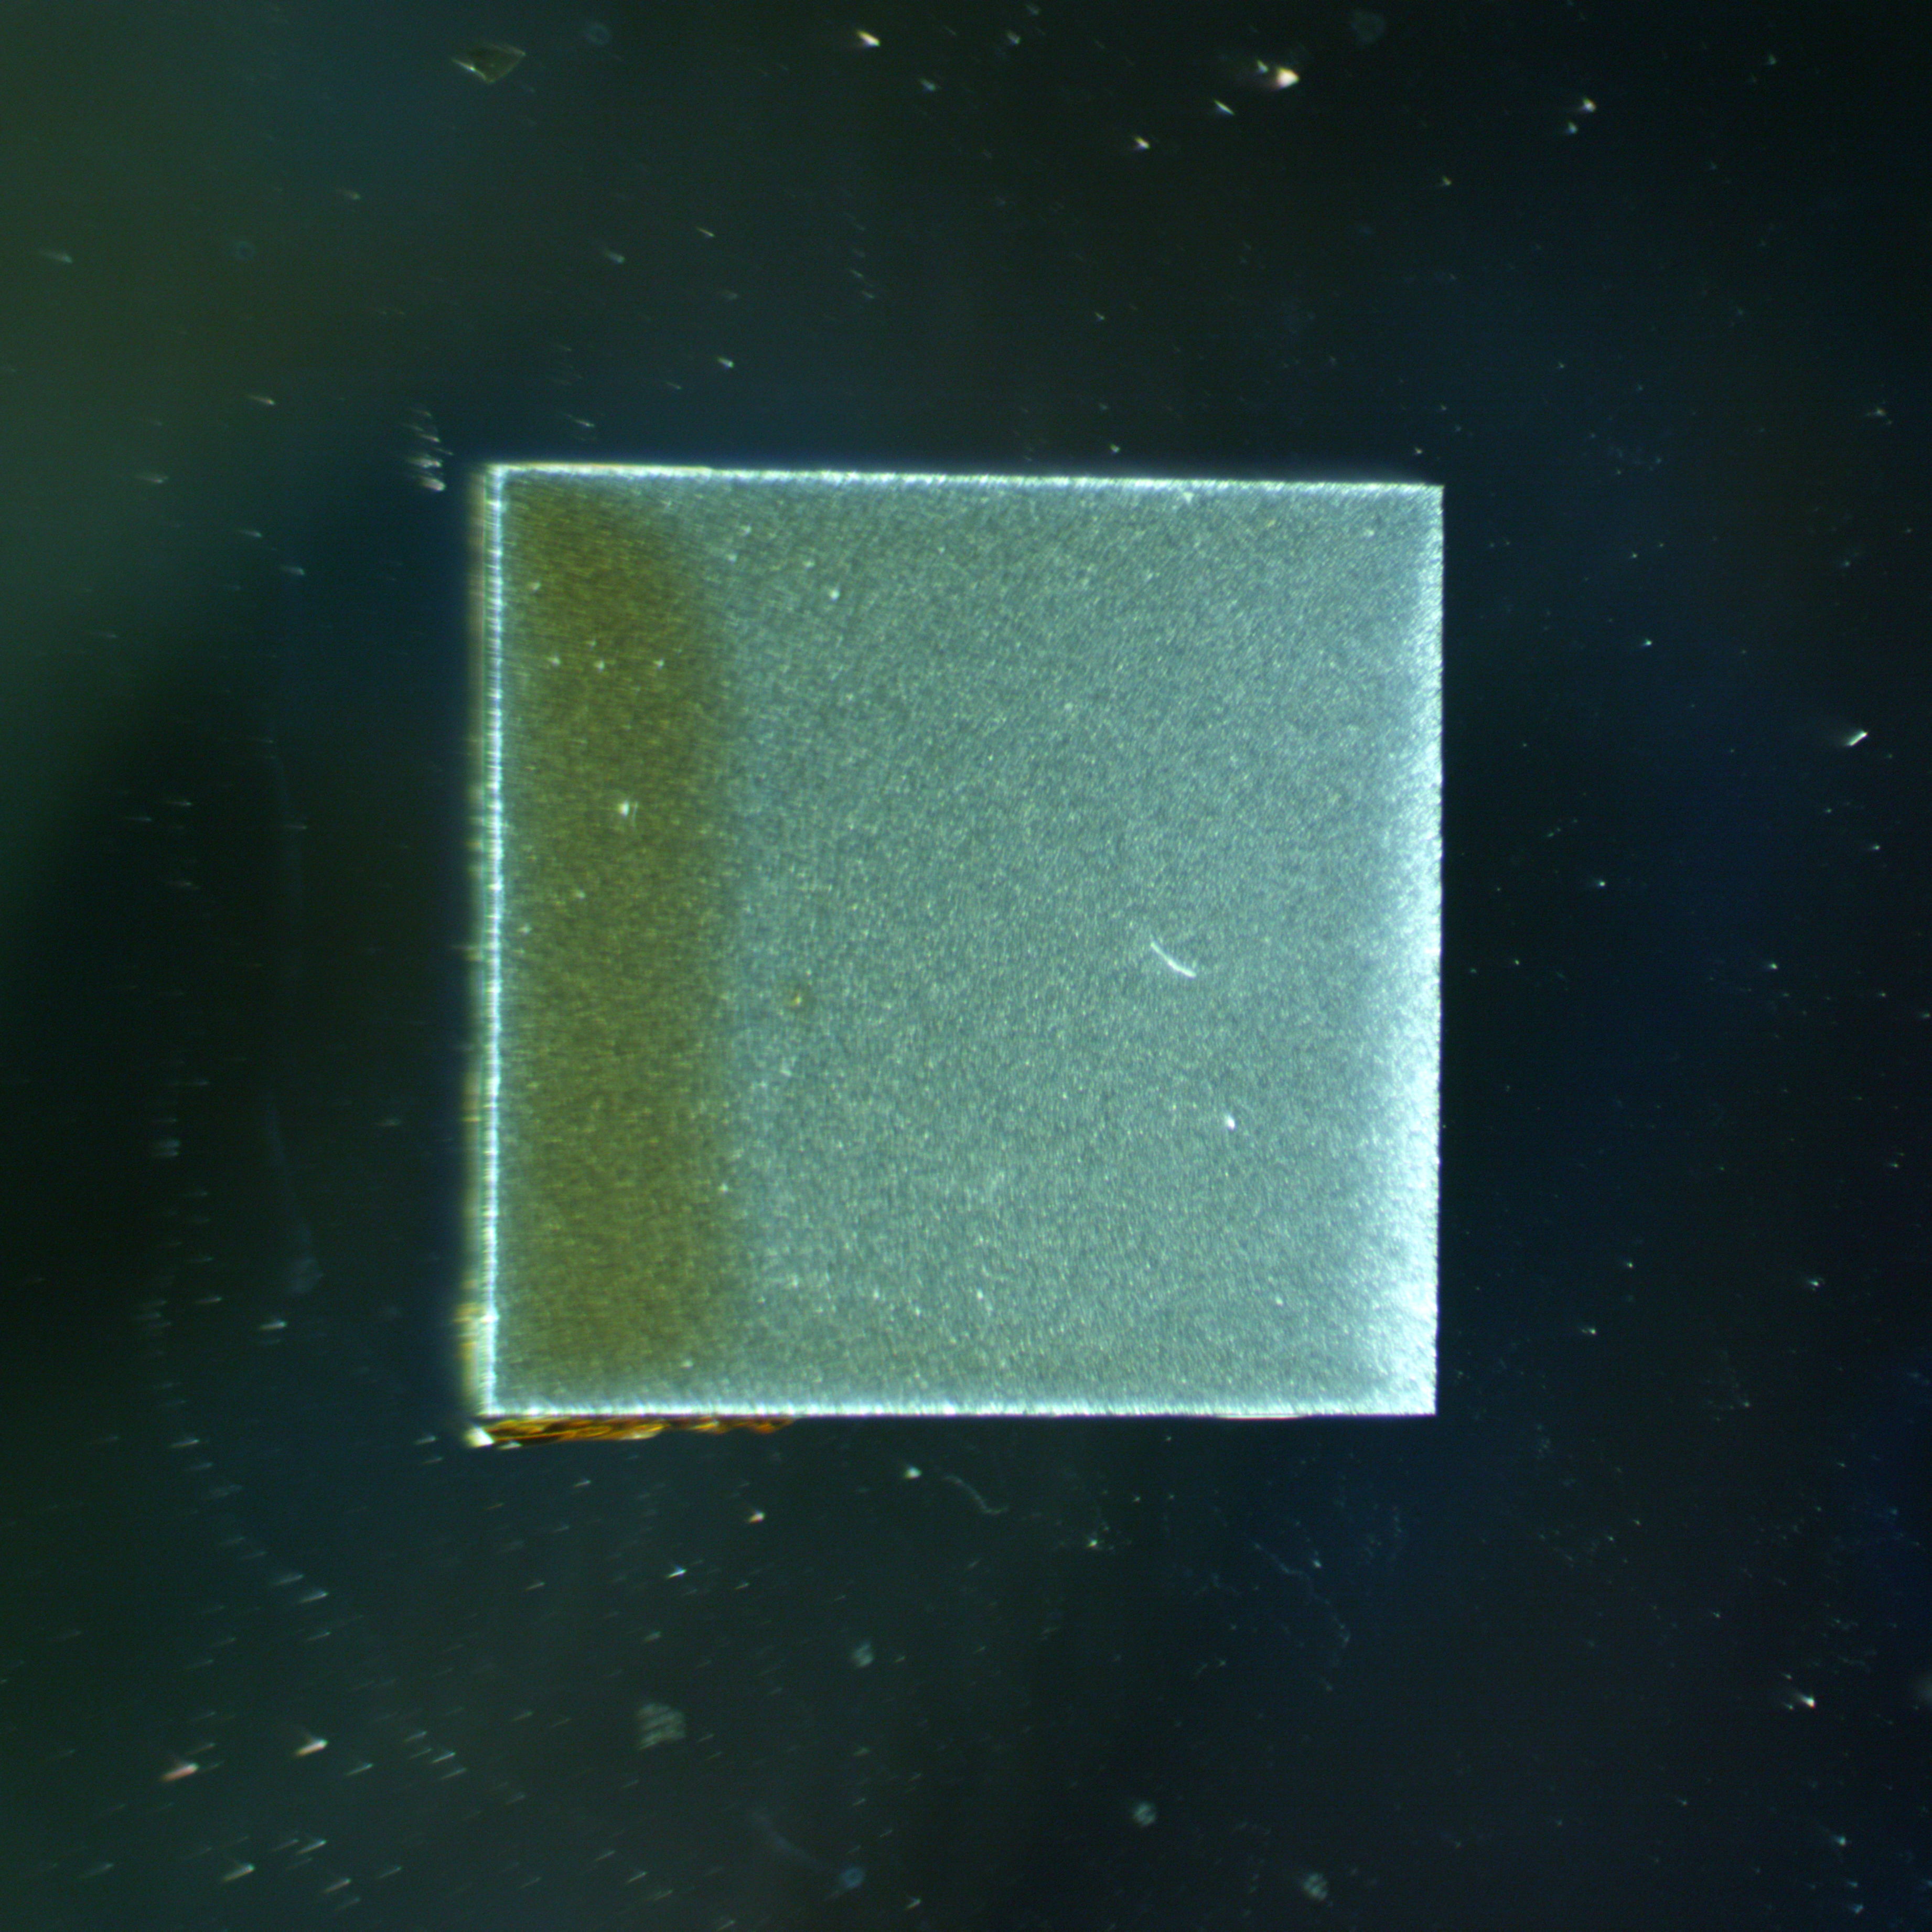
\includegraphics[width=\linewidth]{pics/spincoat/no5/5110.jpg}
        \caption{\textcolor{blue!60!black}{\textbf{Heater 1}}}
    \end{subfigure}
    \hfill
    \begin{subfigure}[t]{0.3\textwidth}
        \centering
        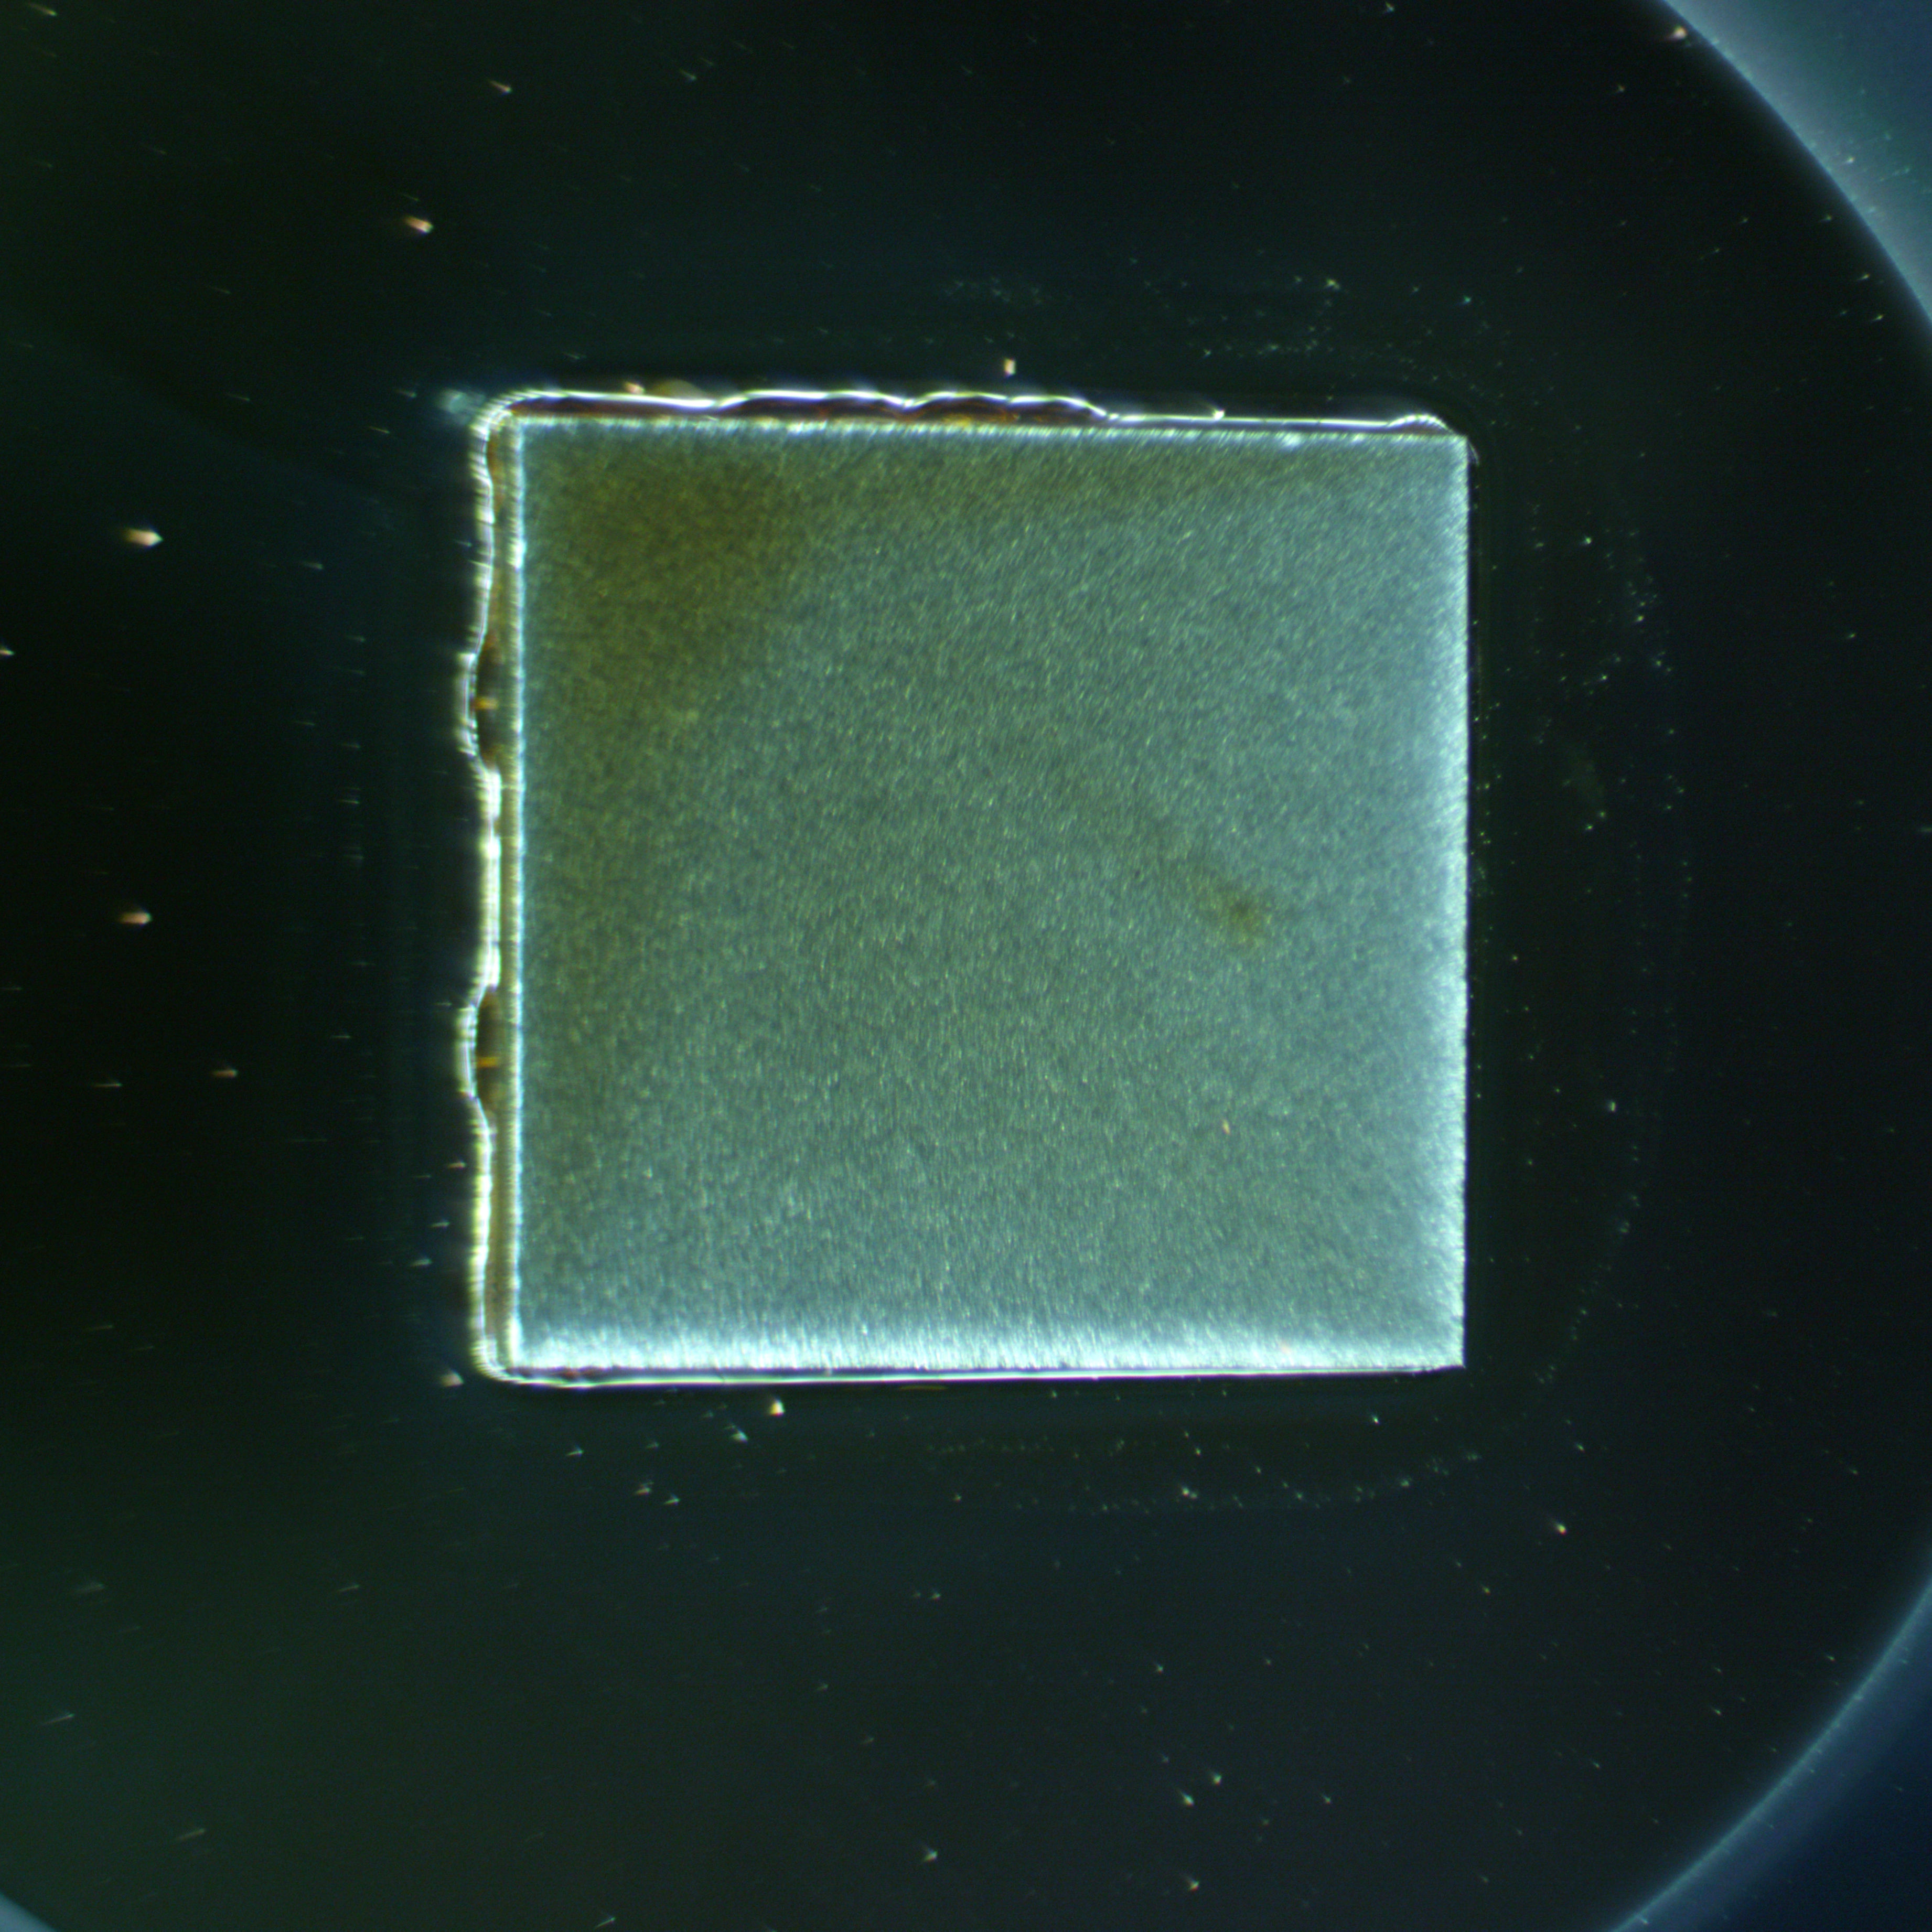
\includegraphics[width=\linewidth]{pics/spincoat/no5/5102.jpg}
        \caption{Heater 2}
    \end{subfigure}
    \hfill
    \begin{subfigure}[t]{0.3\textwidth}
        \centering
        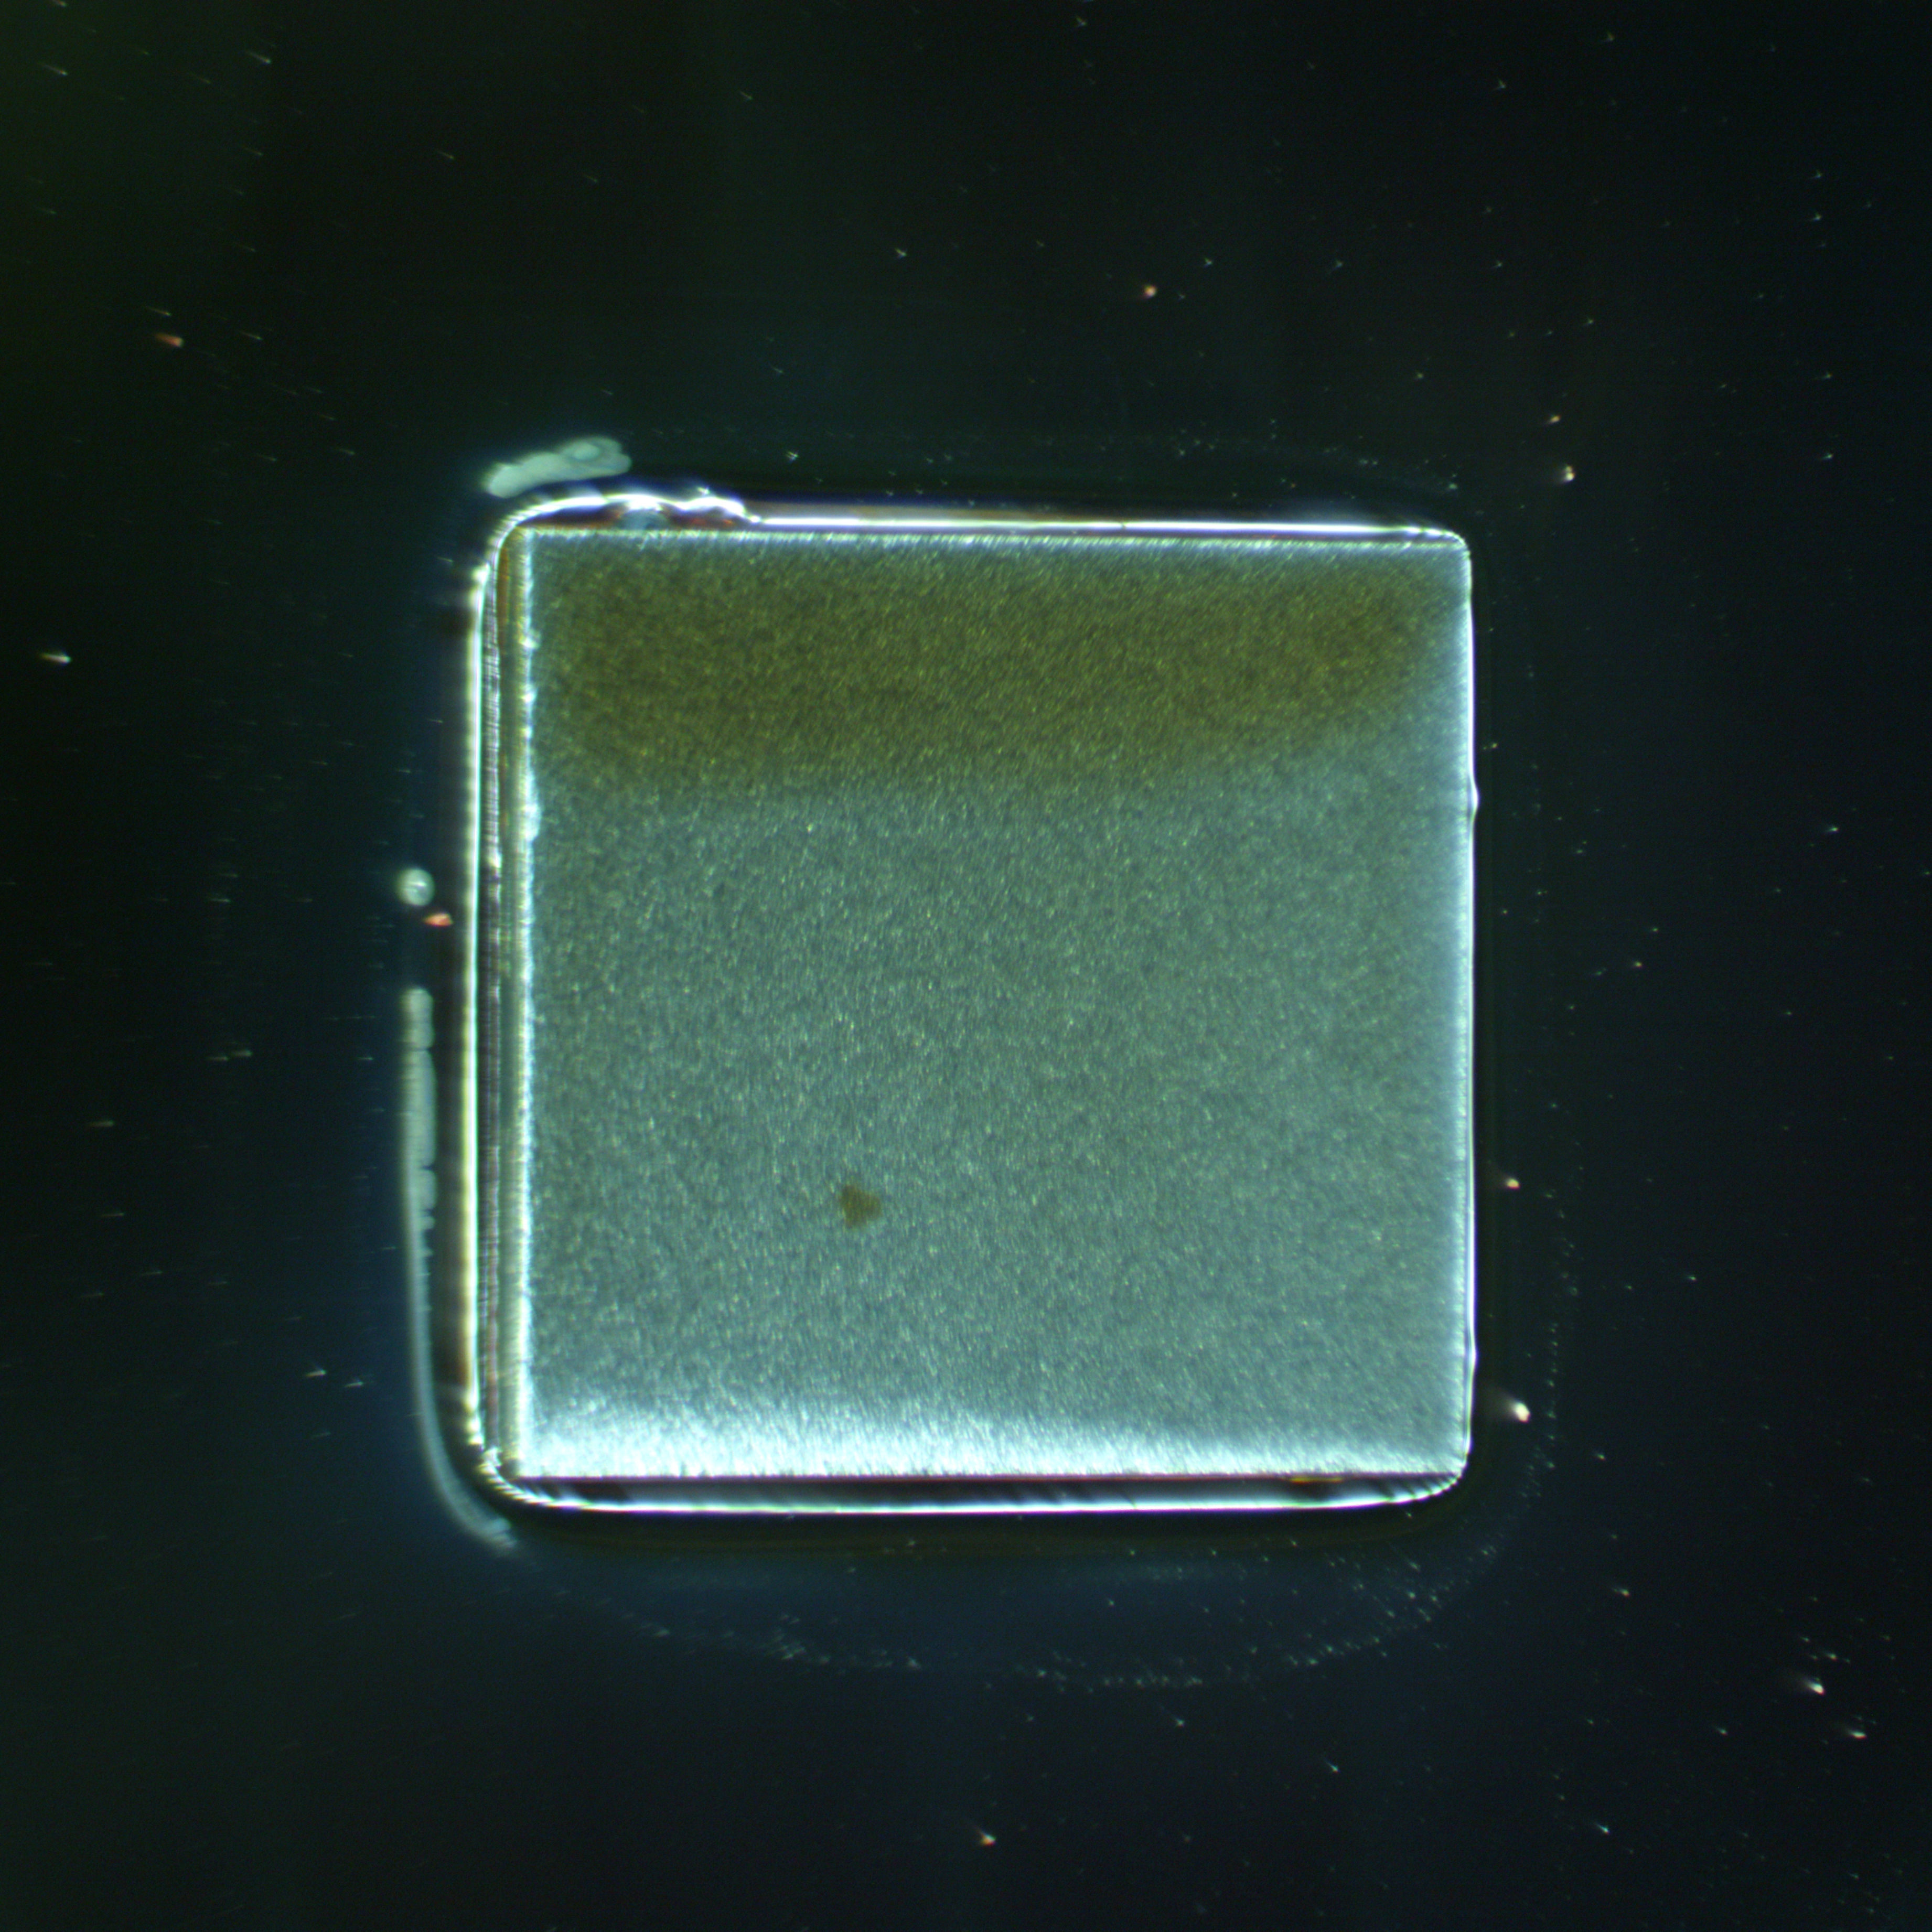
\includegraphics[width=\linewidth]{pics/spincoat/no5/5103.jpg}
        \caption{Heater 3}
    \end{subfigure}

    \vspace{0.8cm}

    % ---------- Row 2 ----------
    \begin{subfigure}[t]{0.3\textwidth}
        \centering
        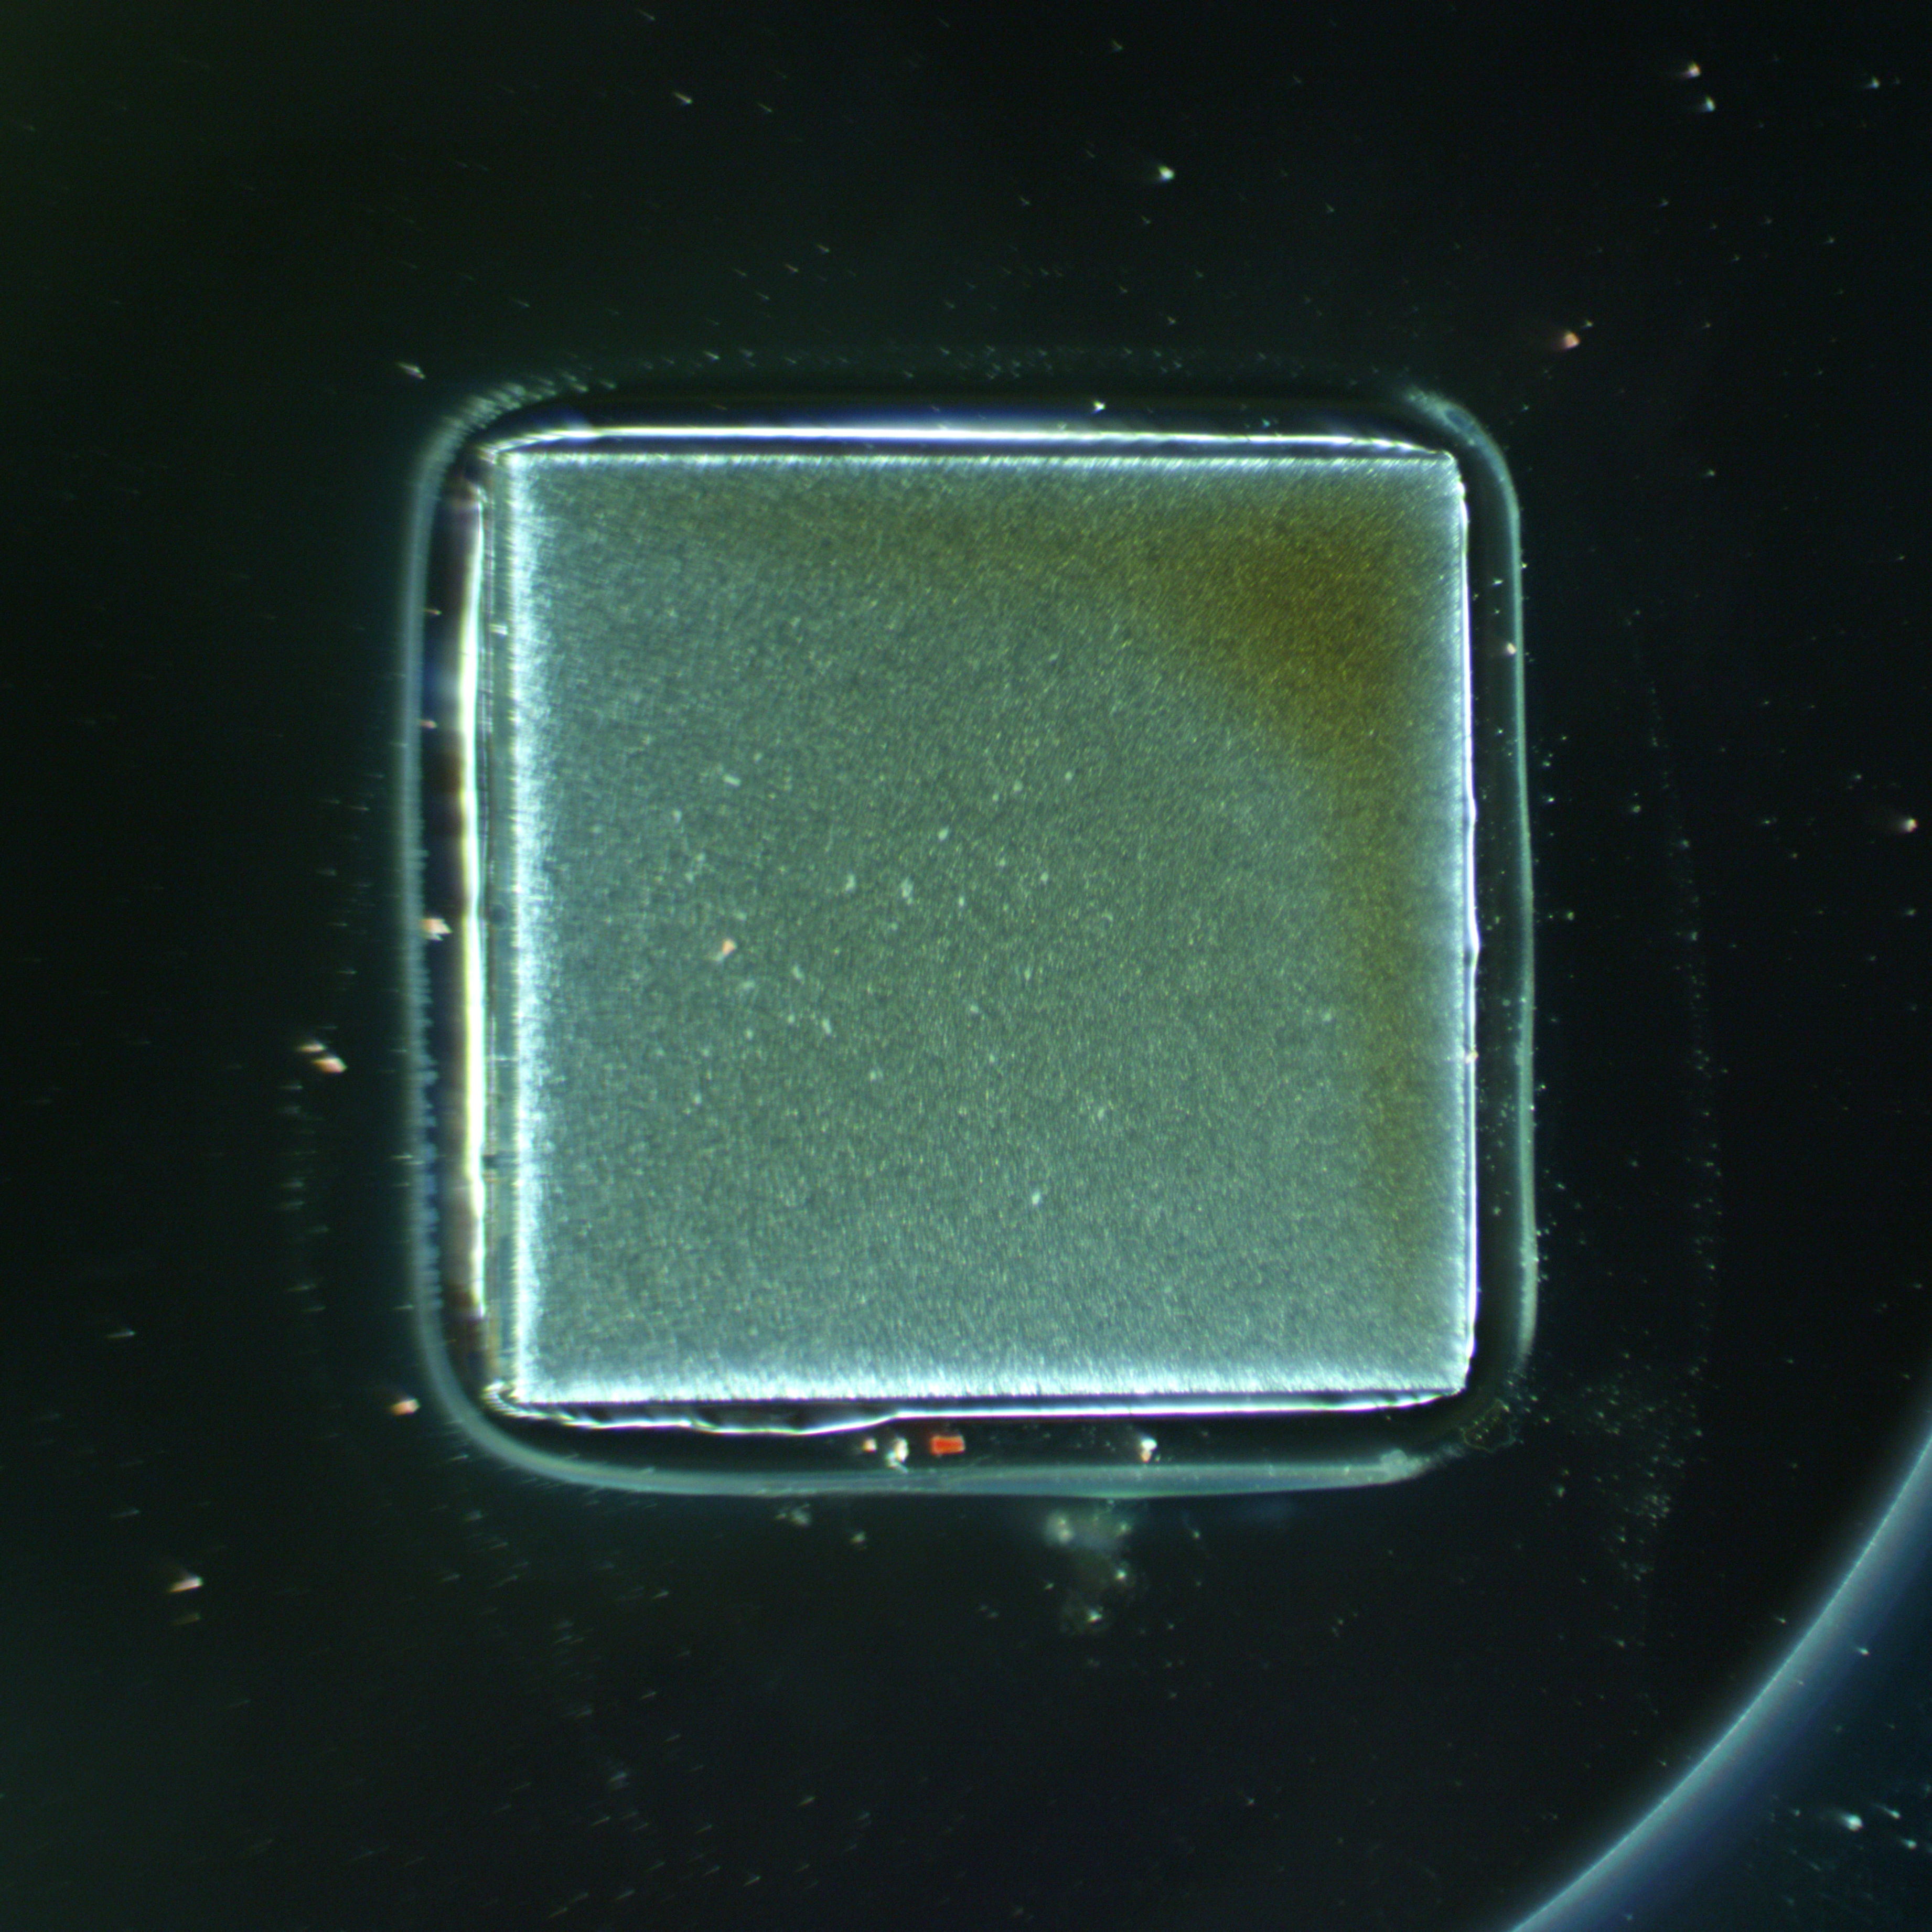
\includegraphics[width=\linewidth]{pics/spincoat/no5/5104.jpg}
        \caption{Heater 4}
    \end{subfigure}
    \hfill
    \begin{subfigure}[t]{0.3\textwidth}
        \centering
        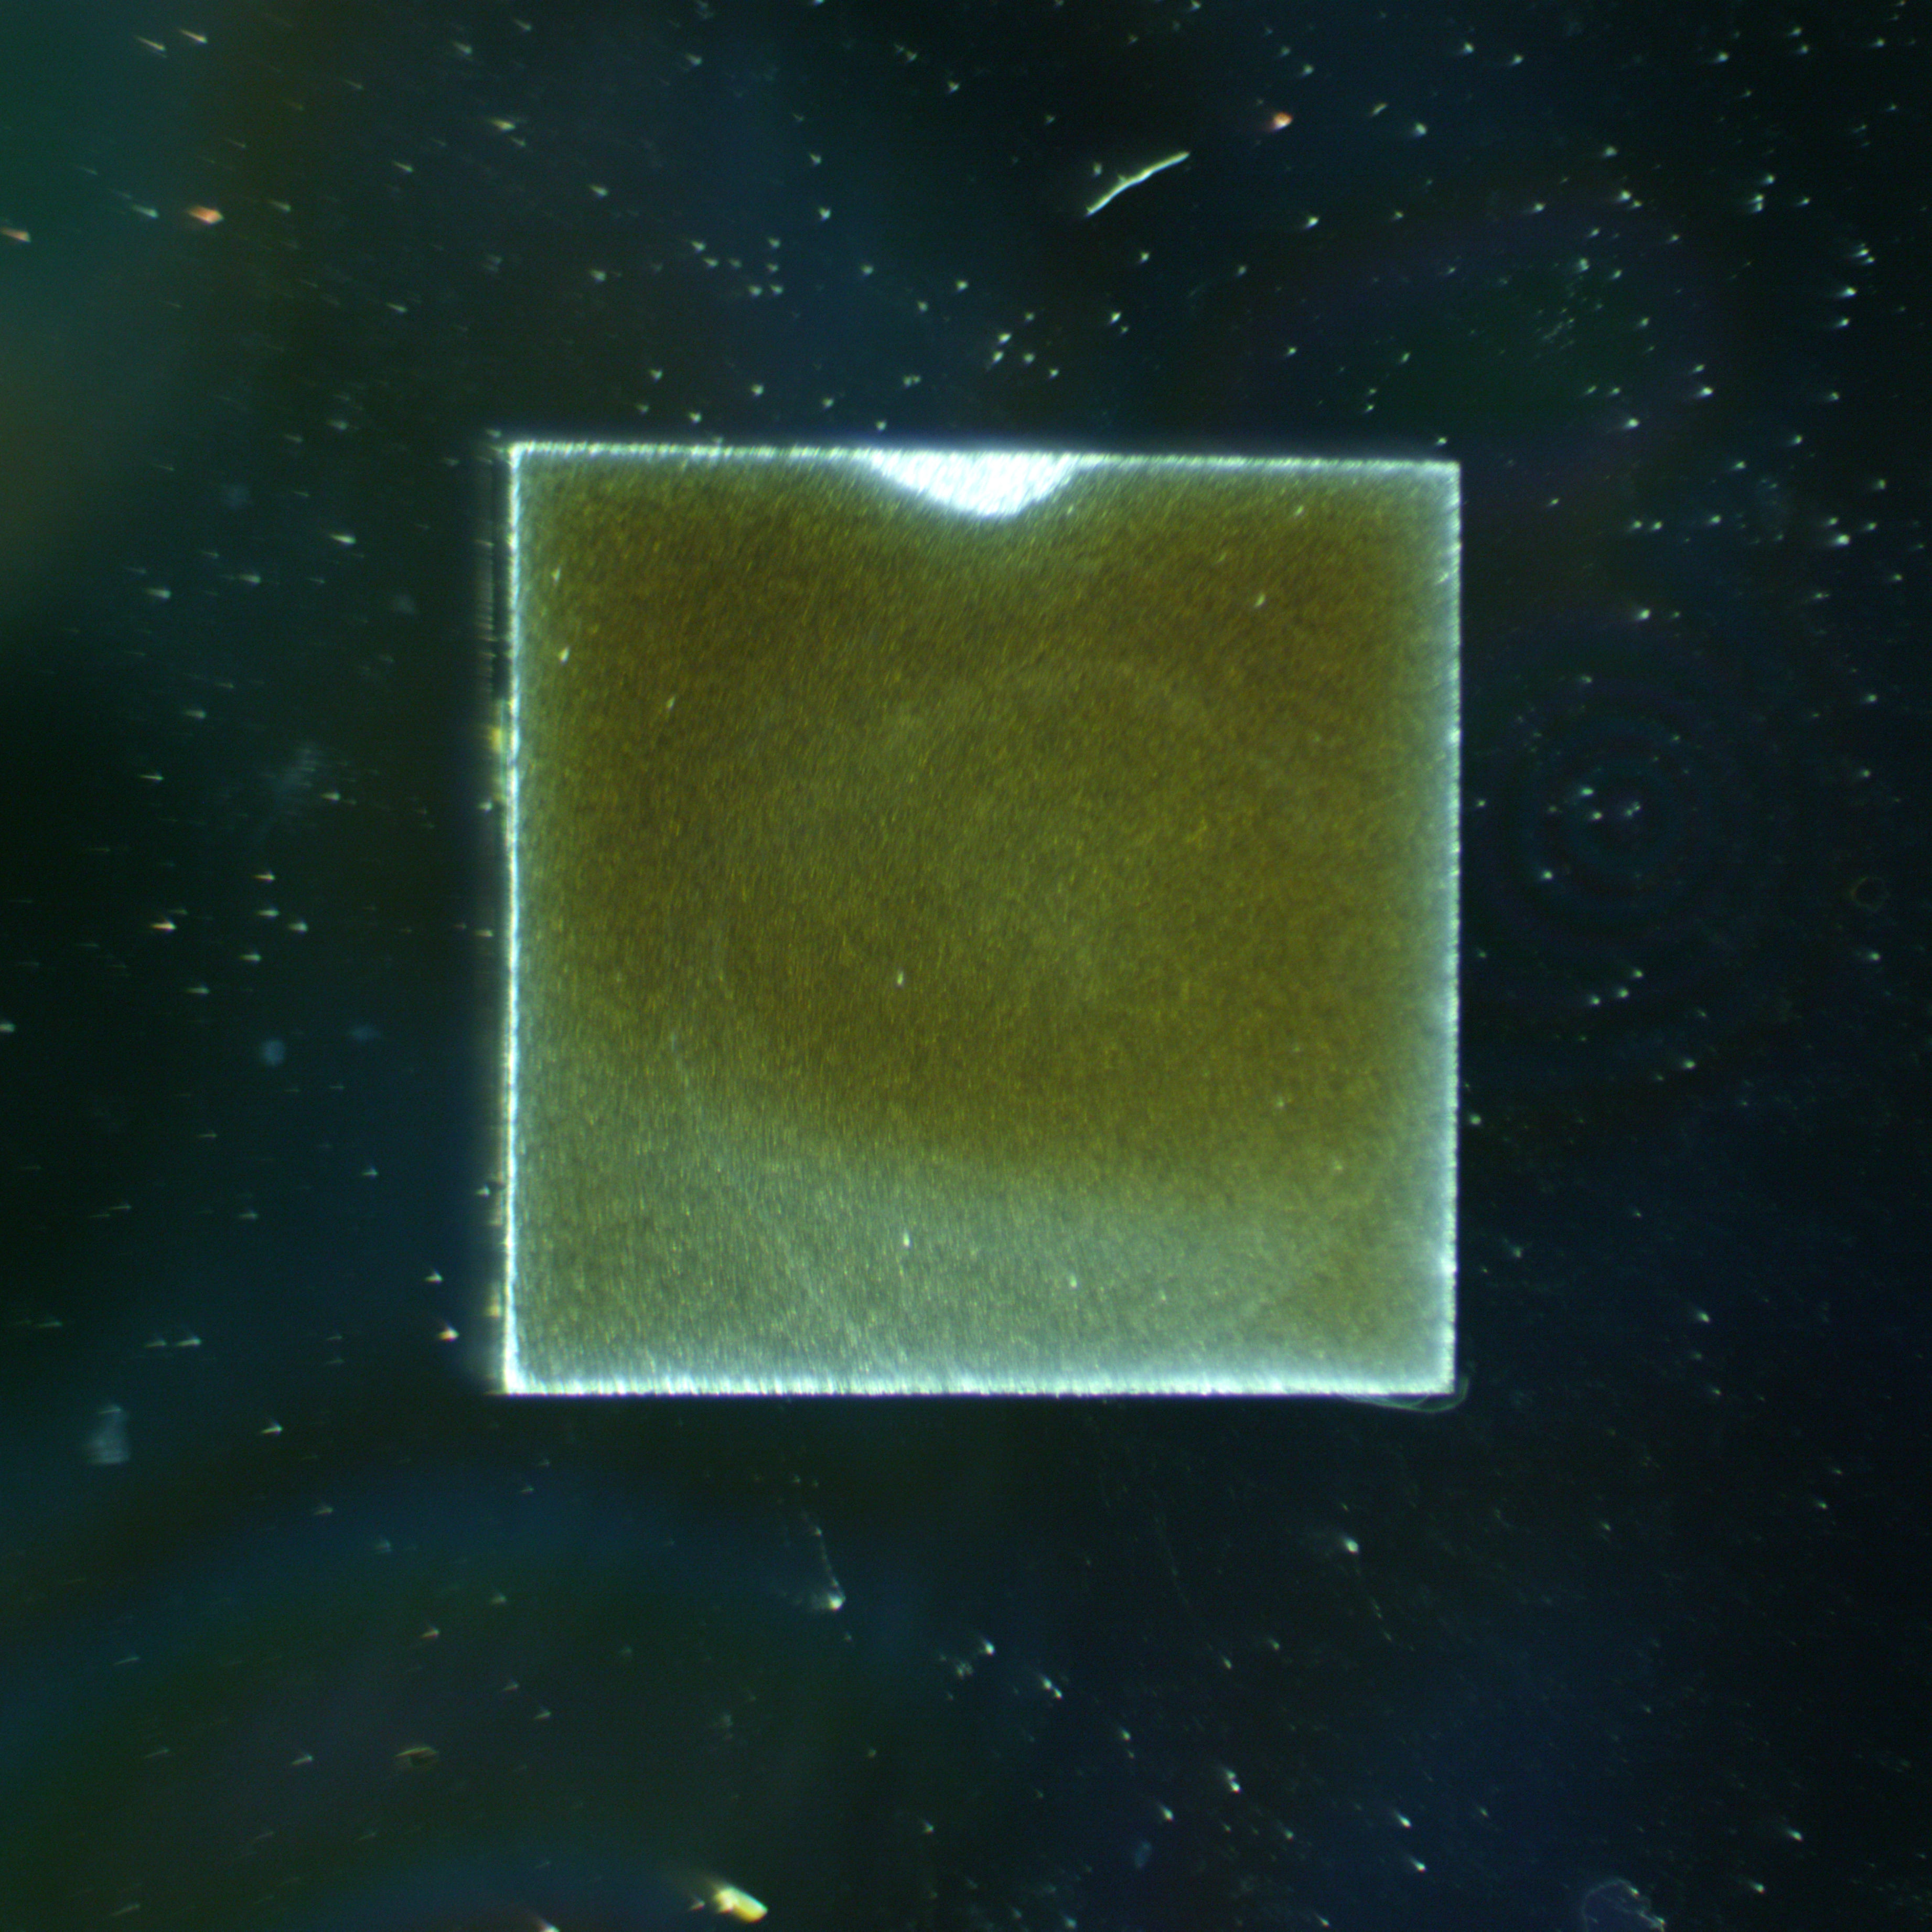
\includegraphics[width=\linewidth]{pics/spincoat/no5/5111.jpg}
        \caption{\textcolor{blue!60!black}{\textbf{Heater 5}}}
    \end{subfigure}
    \hfill
    \begin{subfigure}[t]{0.3\textwidth}
        \centering
        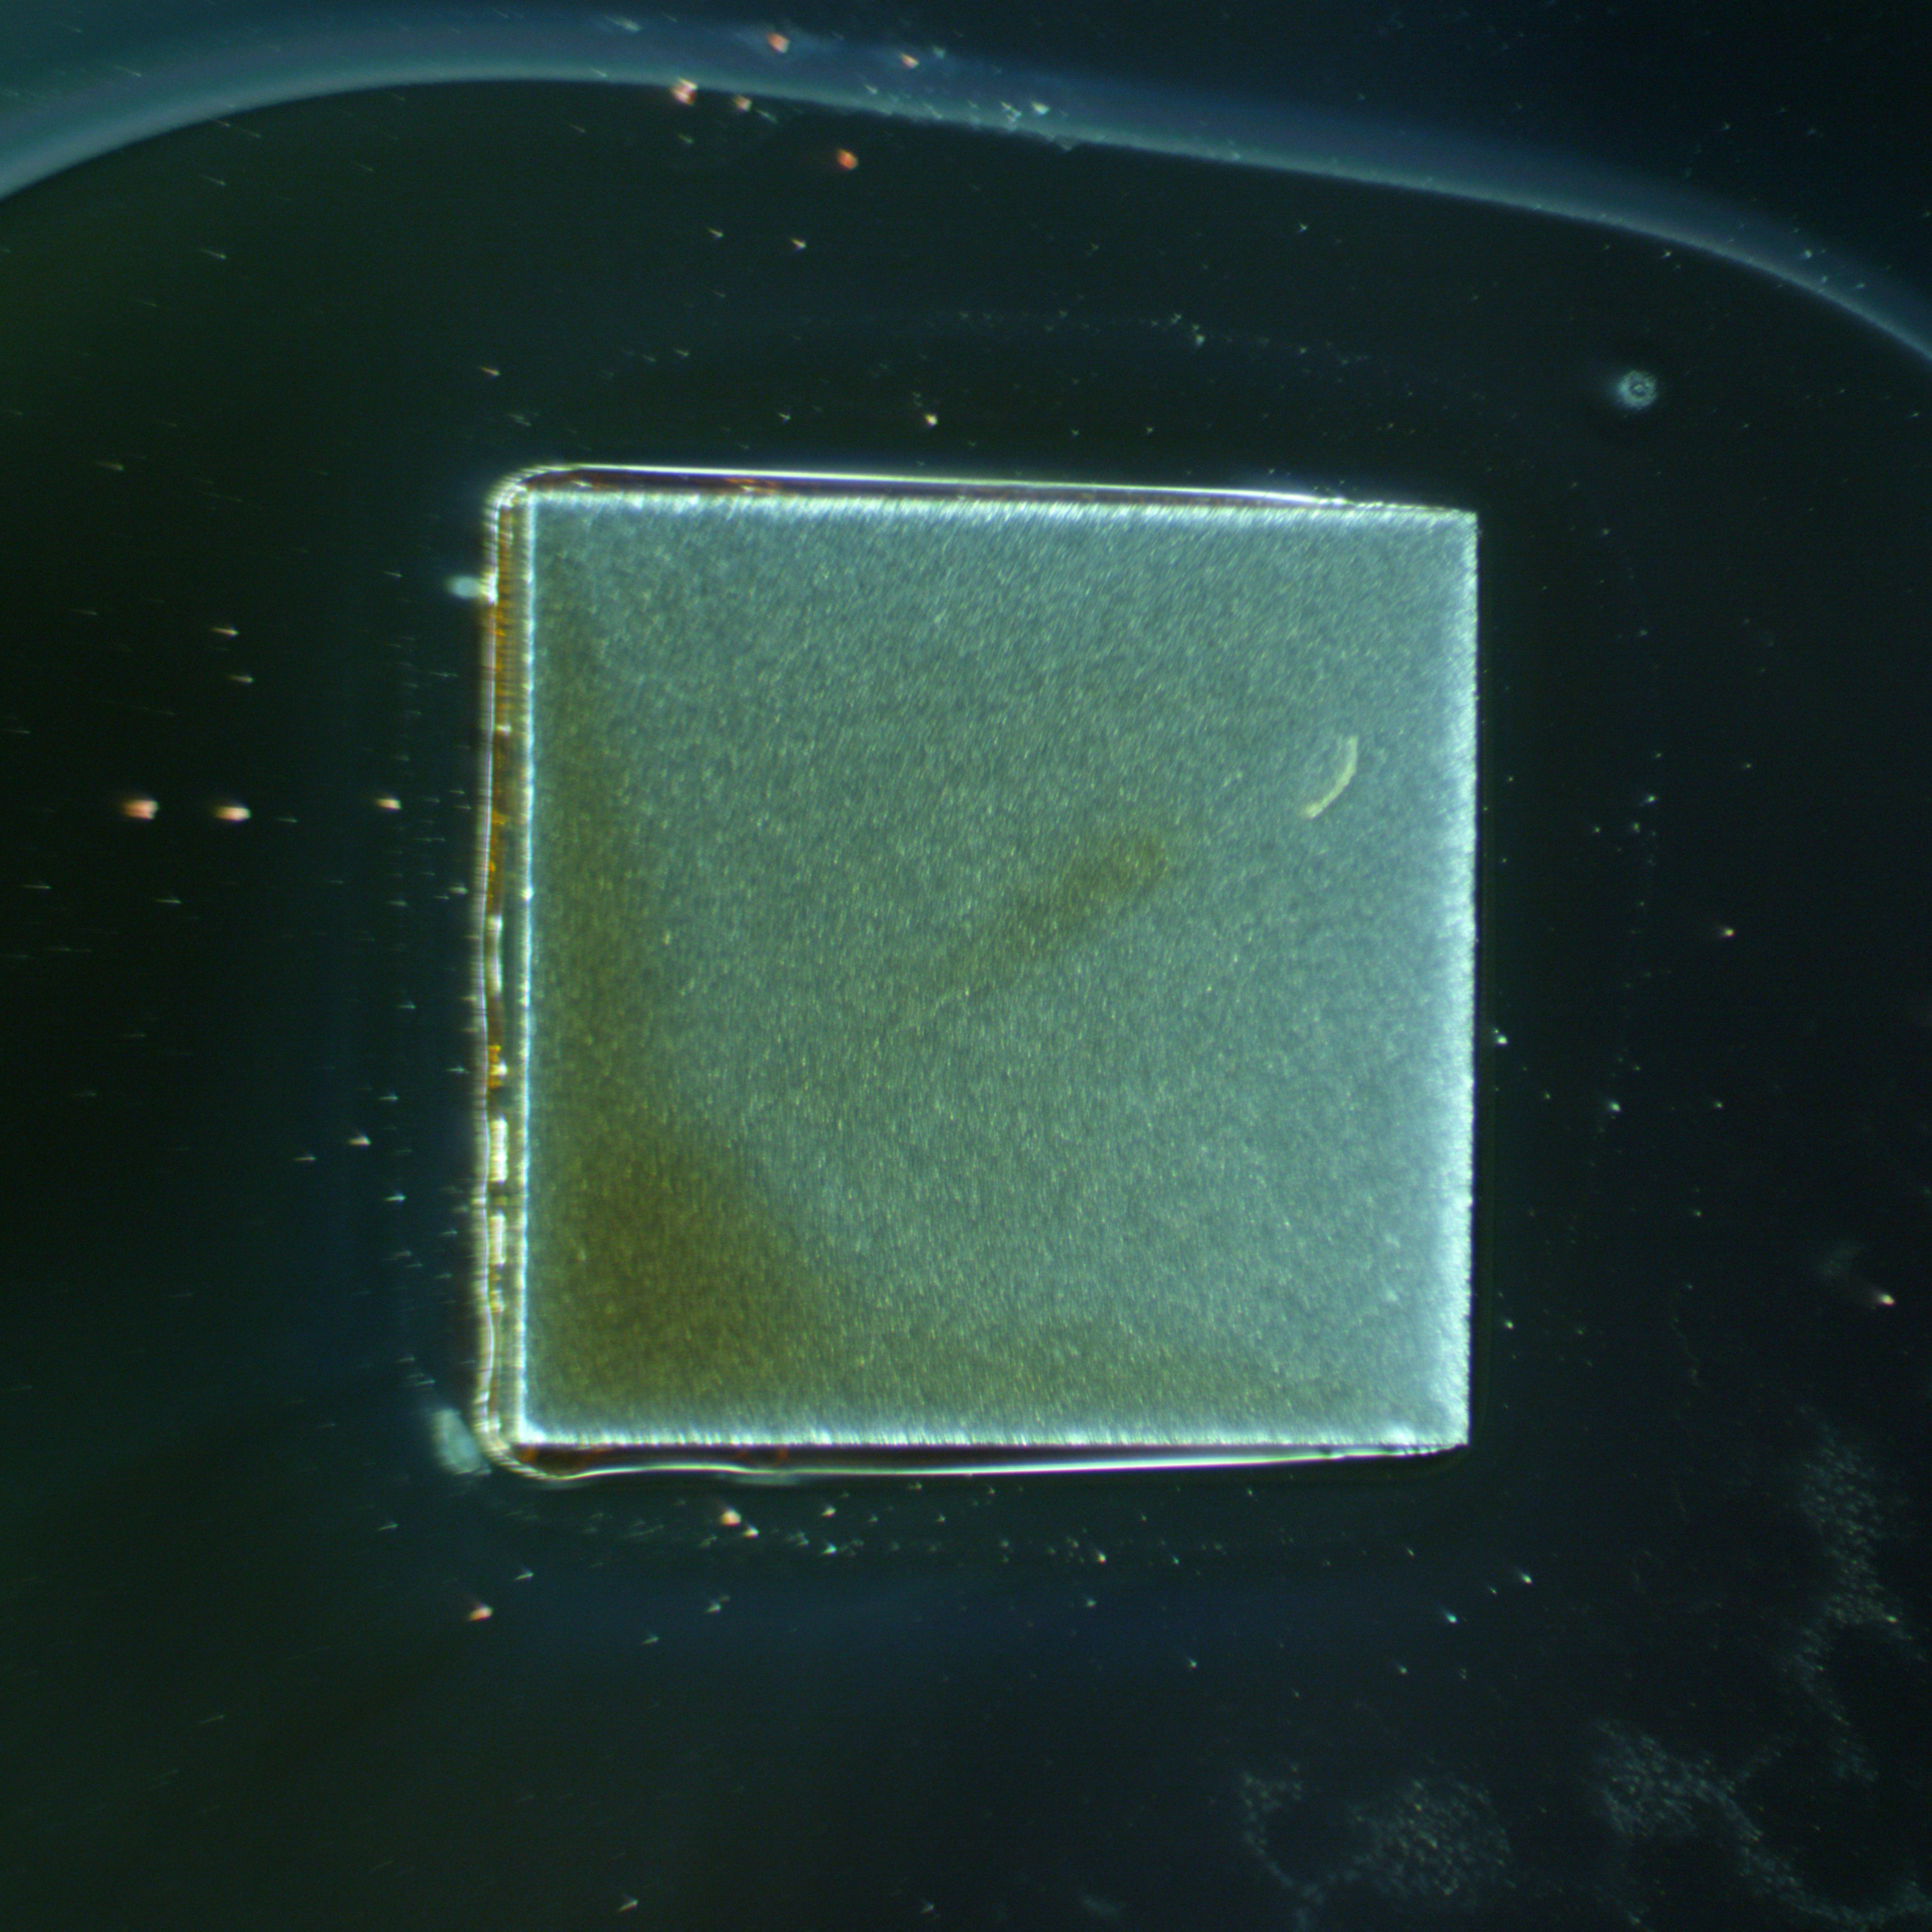
\includegraphics[width=\linewidth]{pics/spincoat/no5/5106.jpg}
        \caption{Heater 6}
    \end{subfigure}

    \vspace{0.8cm}

    % ---------- Row 3 ----------
    \begin{subfigure}[t]{0.3\textwidth}
        \centering
        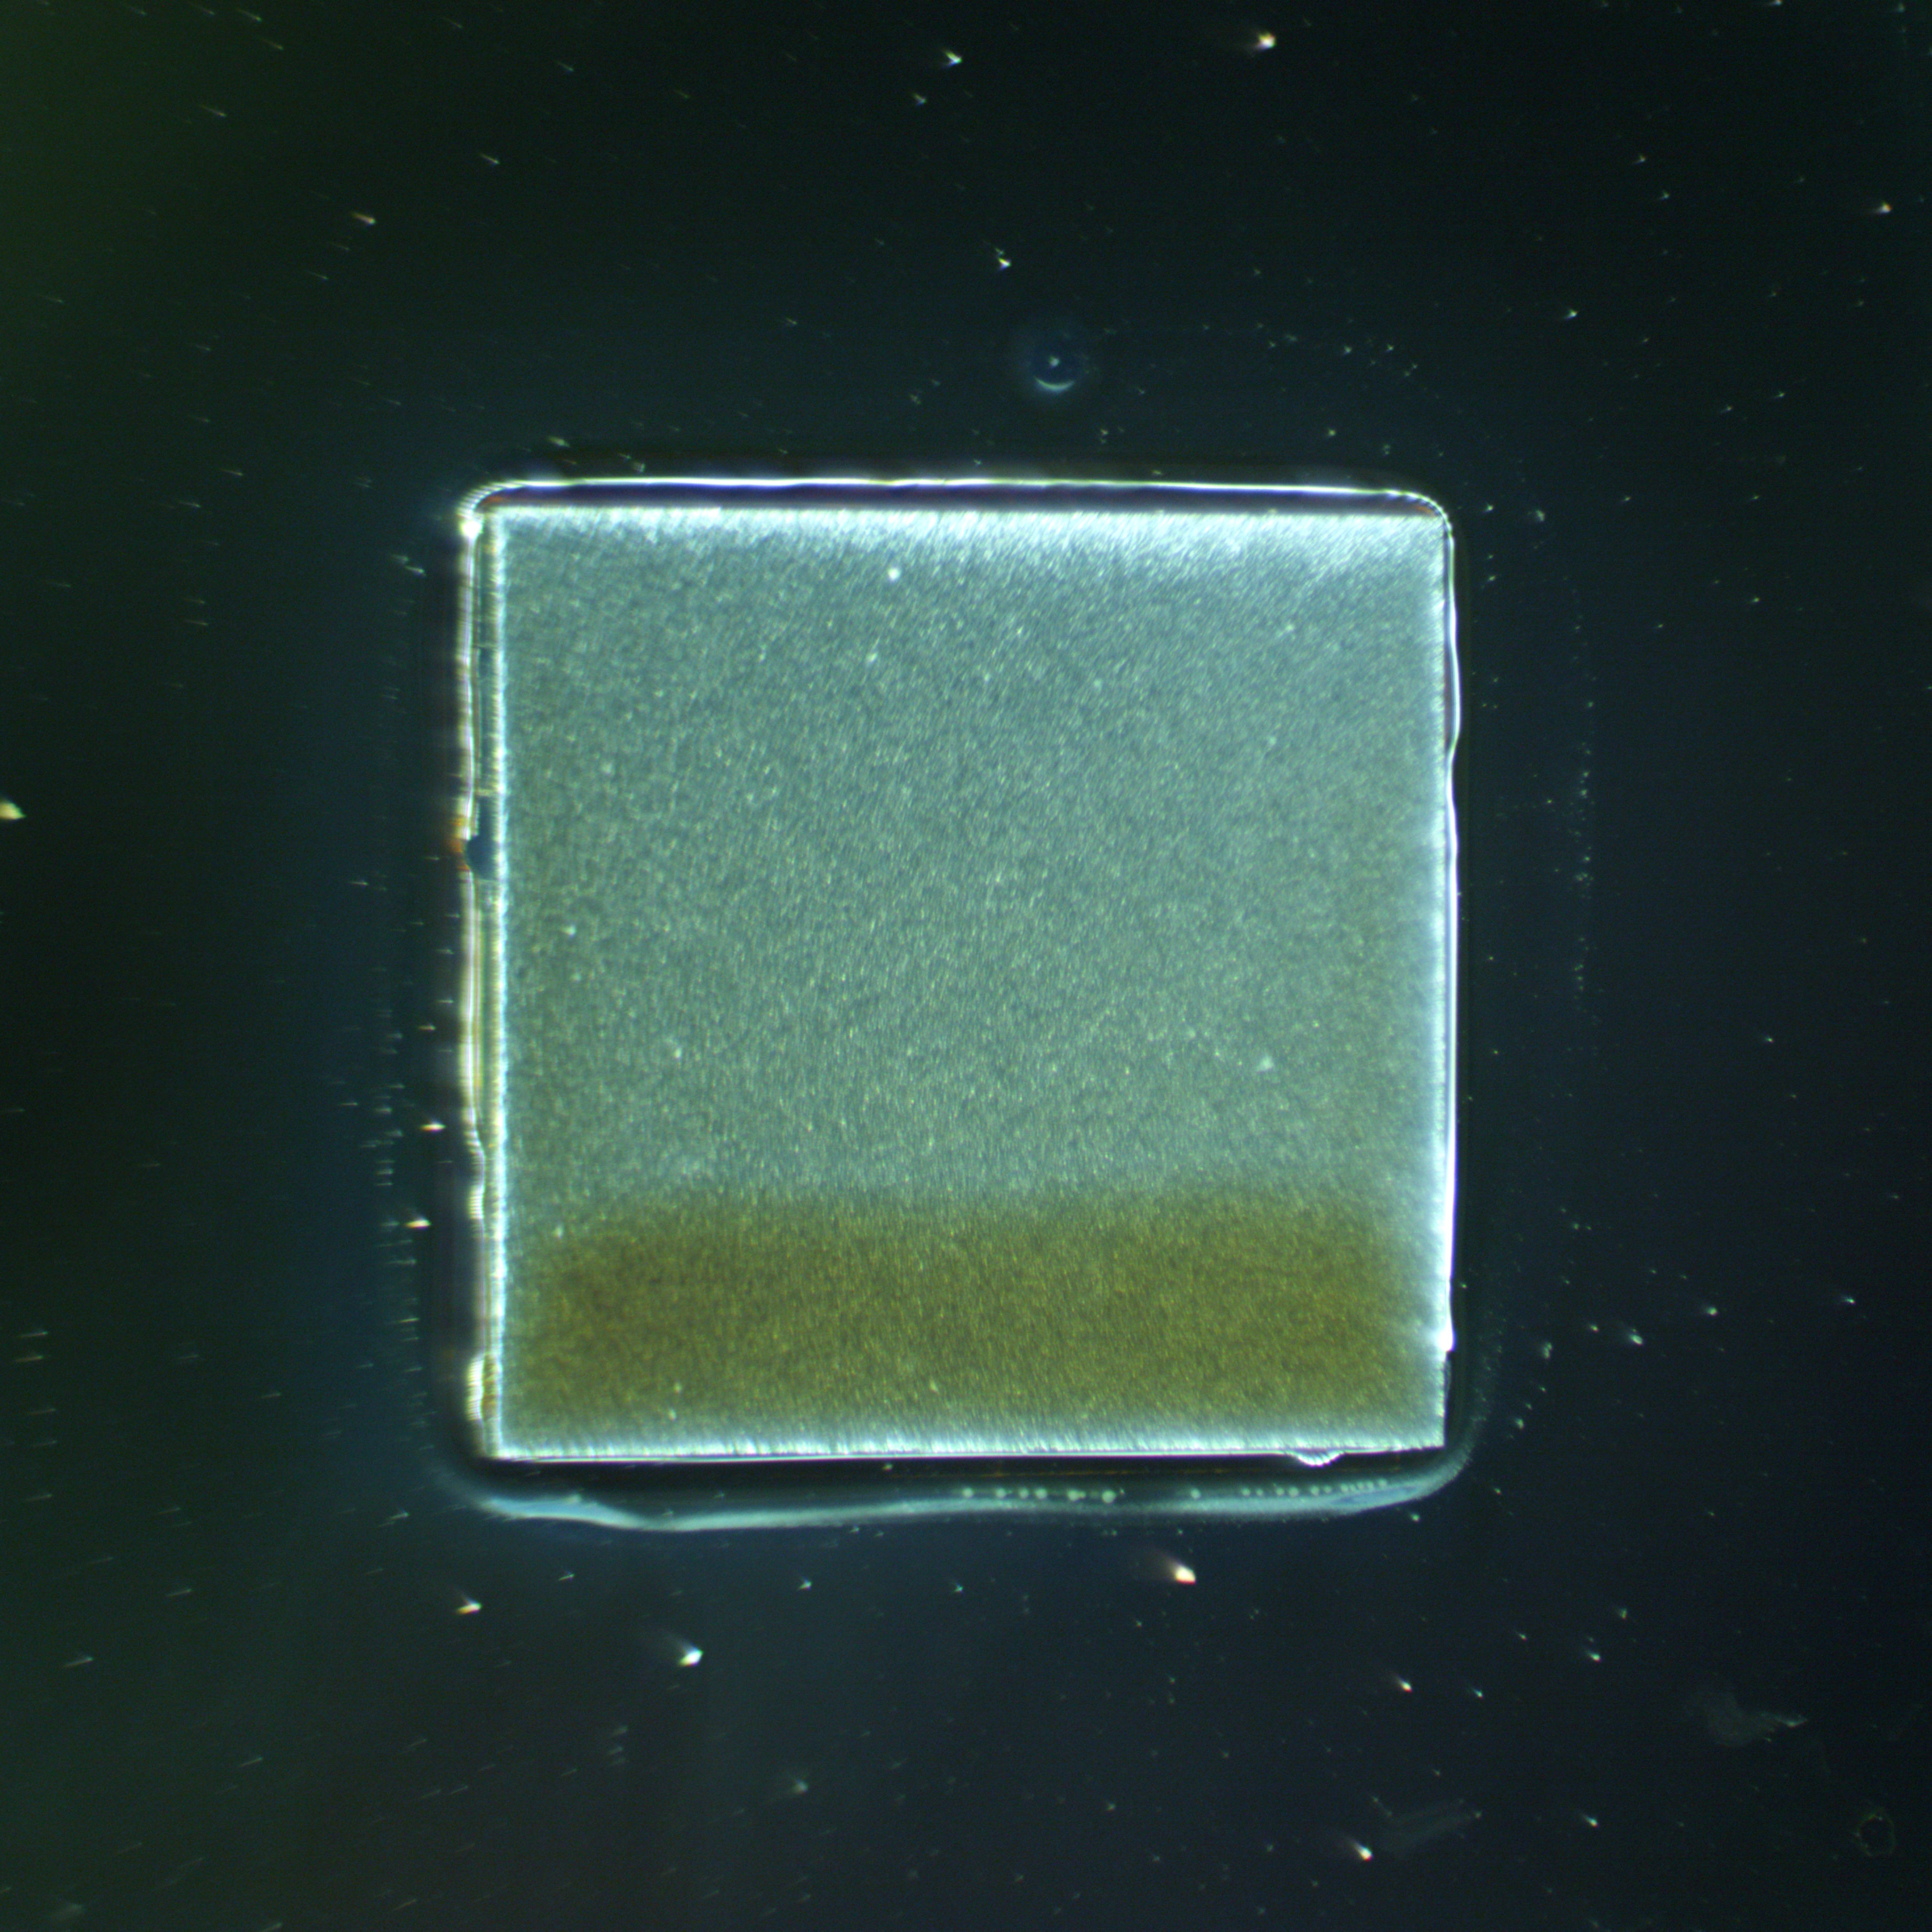
\includegraphics[width=\linewidth]{pics/spincoat/no5/5107.jpg}
        \caption{Heater 7}
    \end{subfigure}
    \hfill
    \begin{subfigure}[t]{0.3\textwidth}
        \centering
        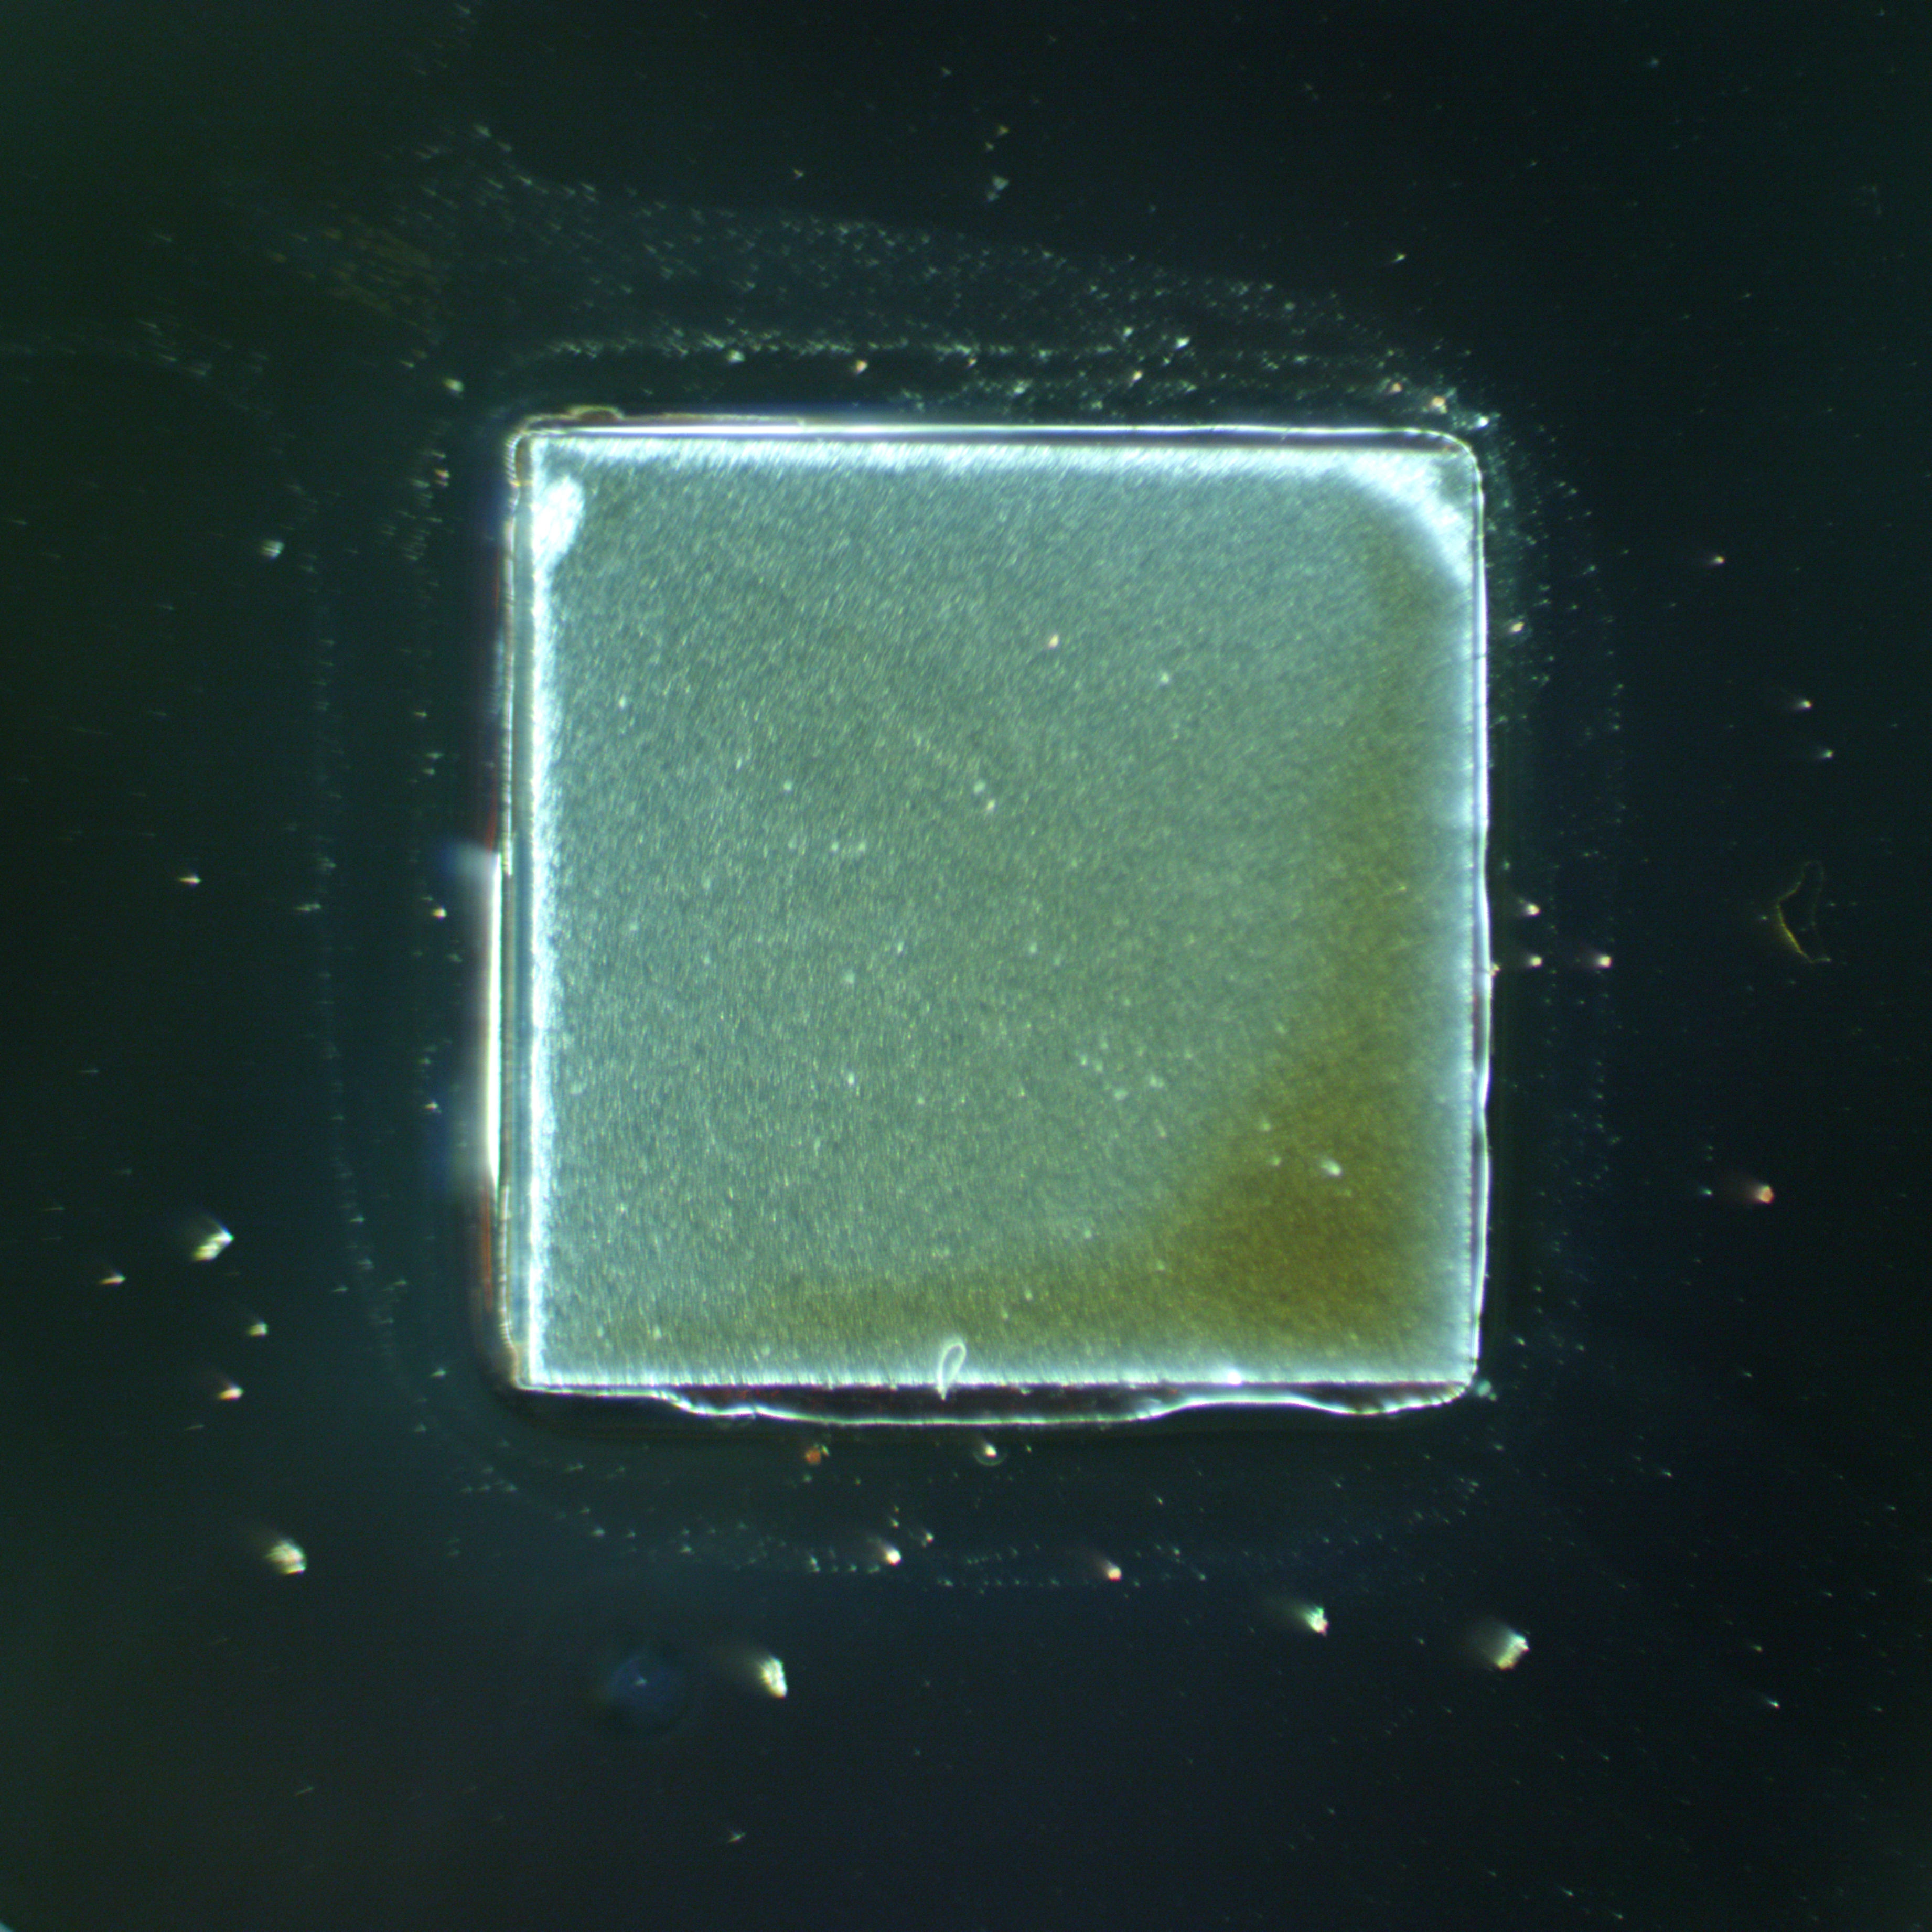
\includegraphics[width=\linewidth]{pics/spincoat/no5/5108.jpg}
        \caption{Heater 8}
    \end{subfigure}
    \hfill
    \begin{subfigure}[t]{0.3\textwidth}
        \centering
        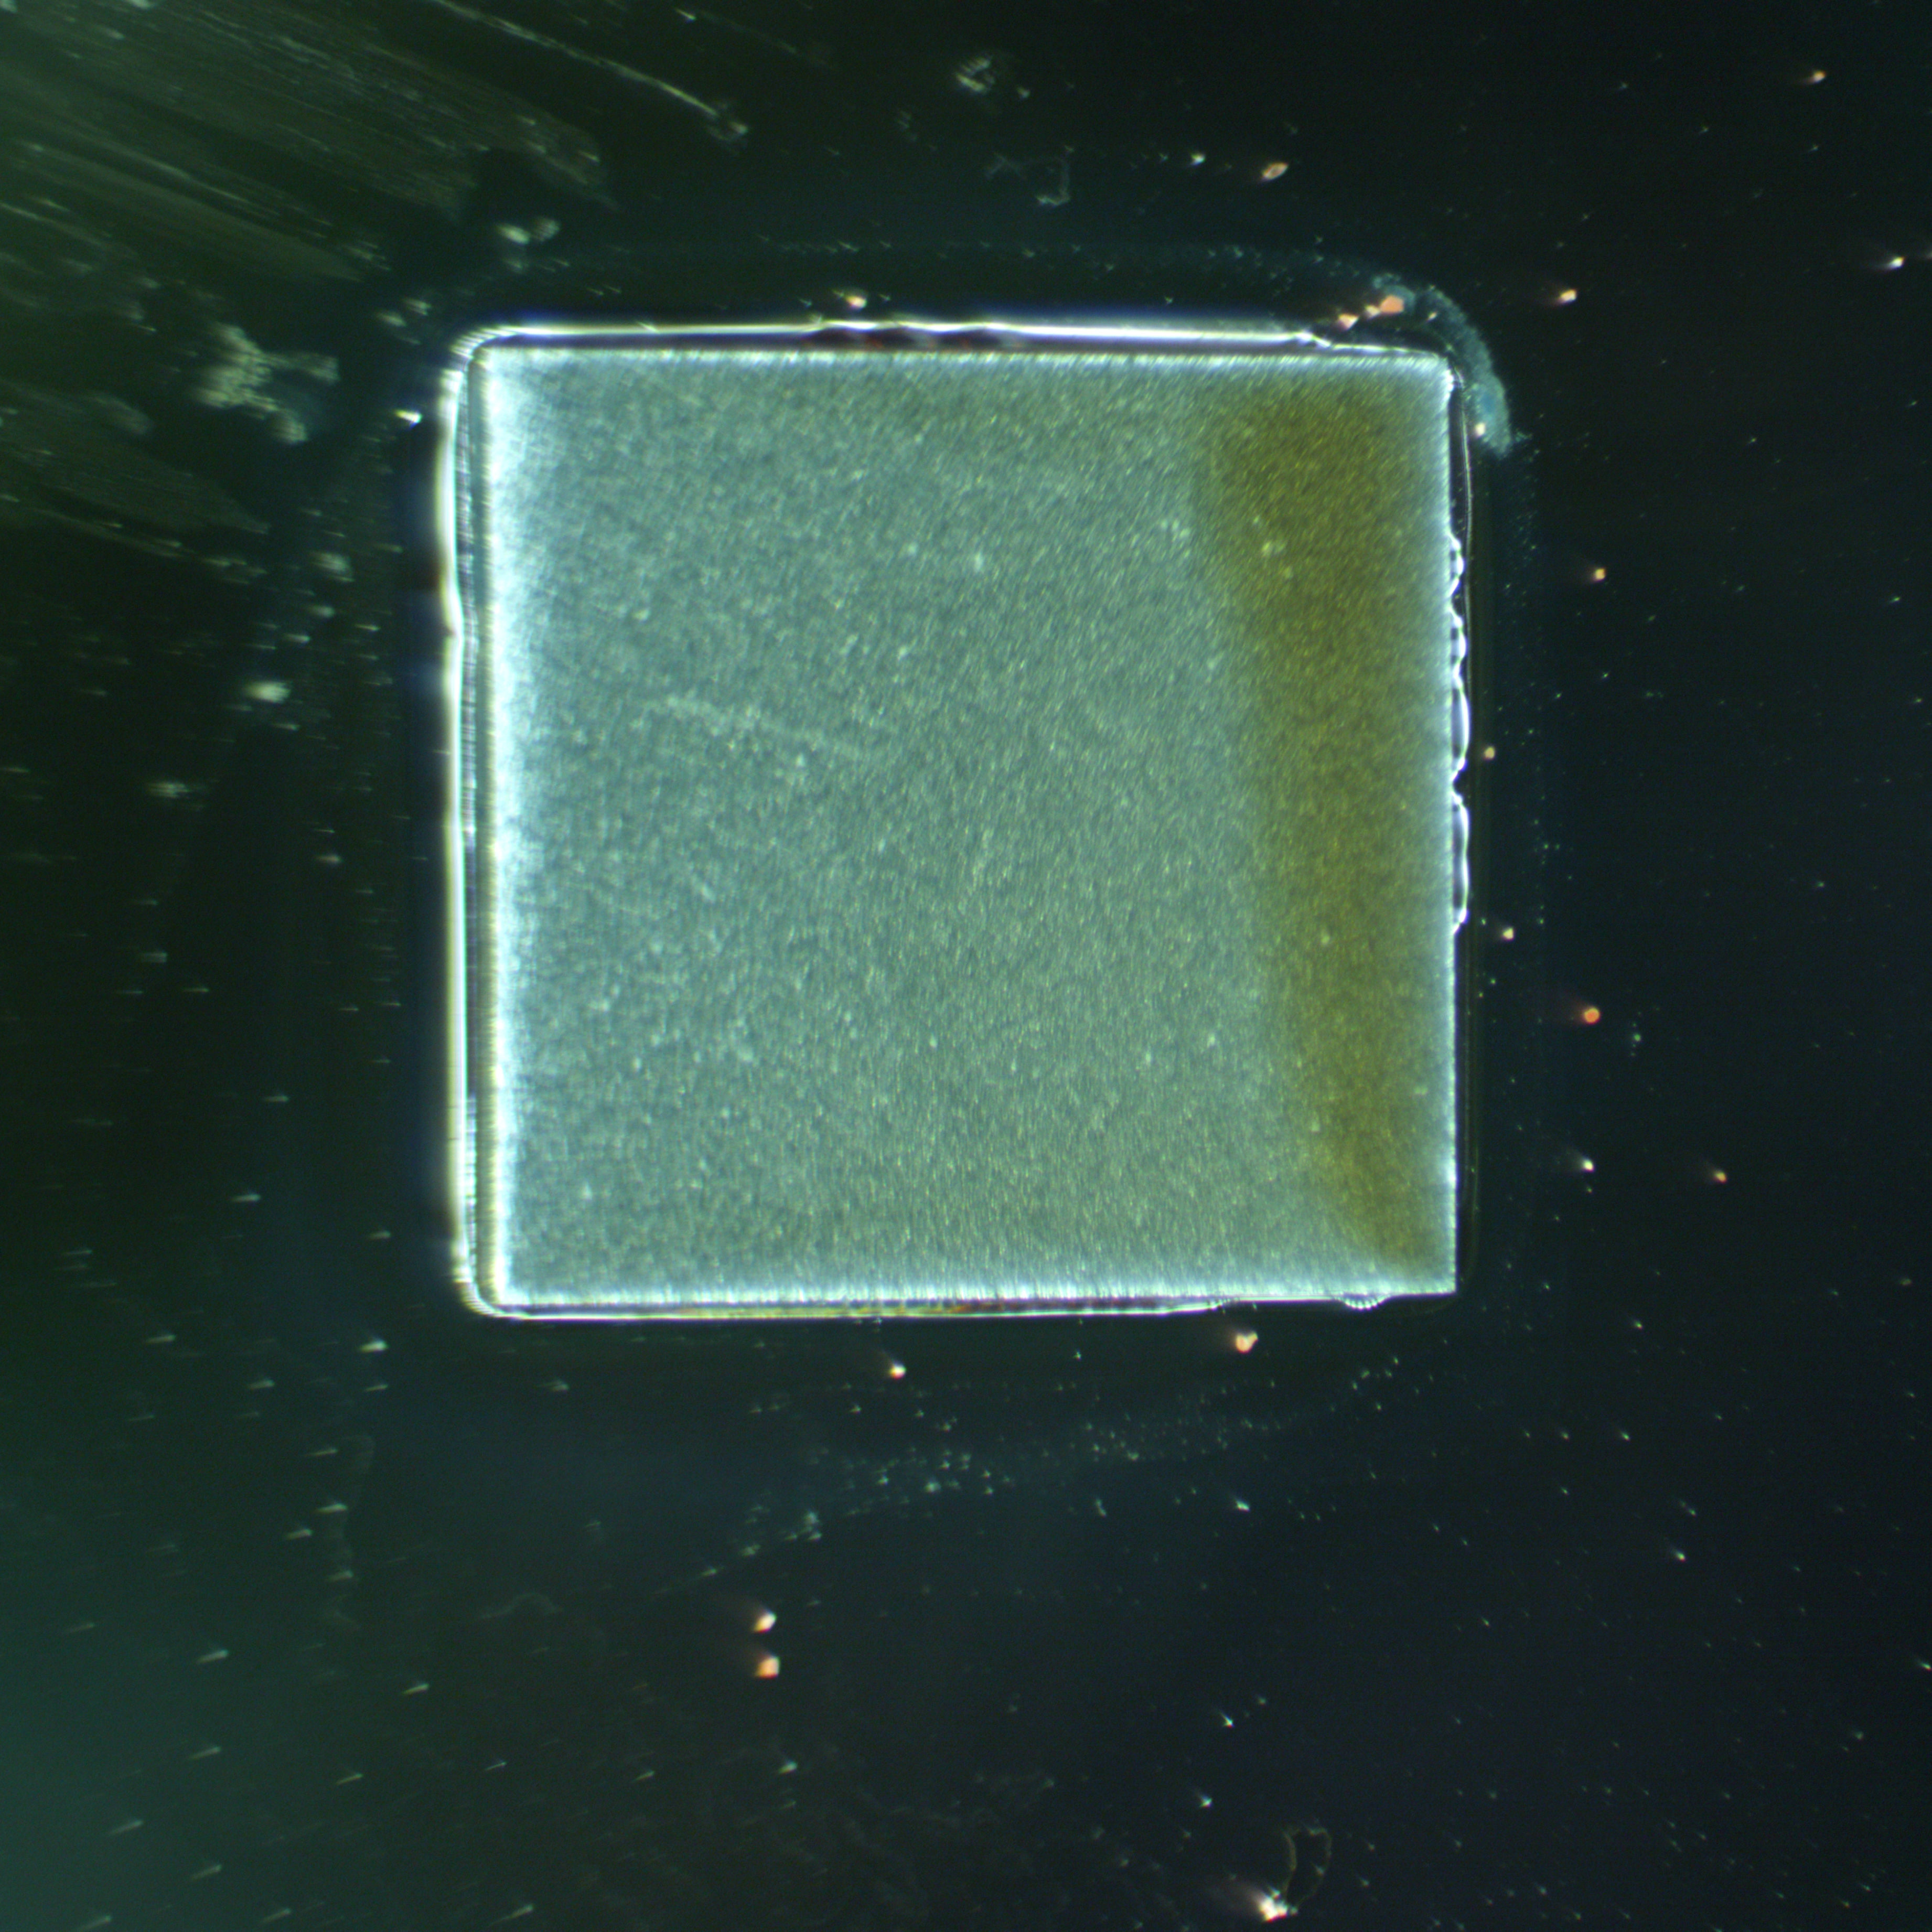
\includegraphics[width=\linewidth]{pics/spincoat/no5/5109.jpg}
        \caption{Heater 9}
    \end{subfigure}

    \caption[Optical Images of the Heater in Passivation Test \#5]{Optical images of the nine Heater of the coating test \#5. The two heaters that could be removed from the glue are highlighted in blue.}
    \label{fig:PT5}
\end{figure}
%================================================================================
%================================================================================
\begin{figure}[htbp]
    \centering

    % ---------- Row 1 ----------
    \begin{subfigure}[t]{0.3\textwidth}
        \centering
        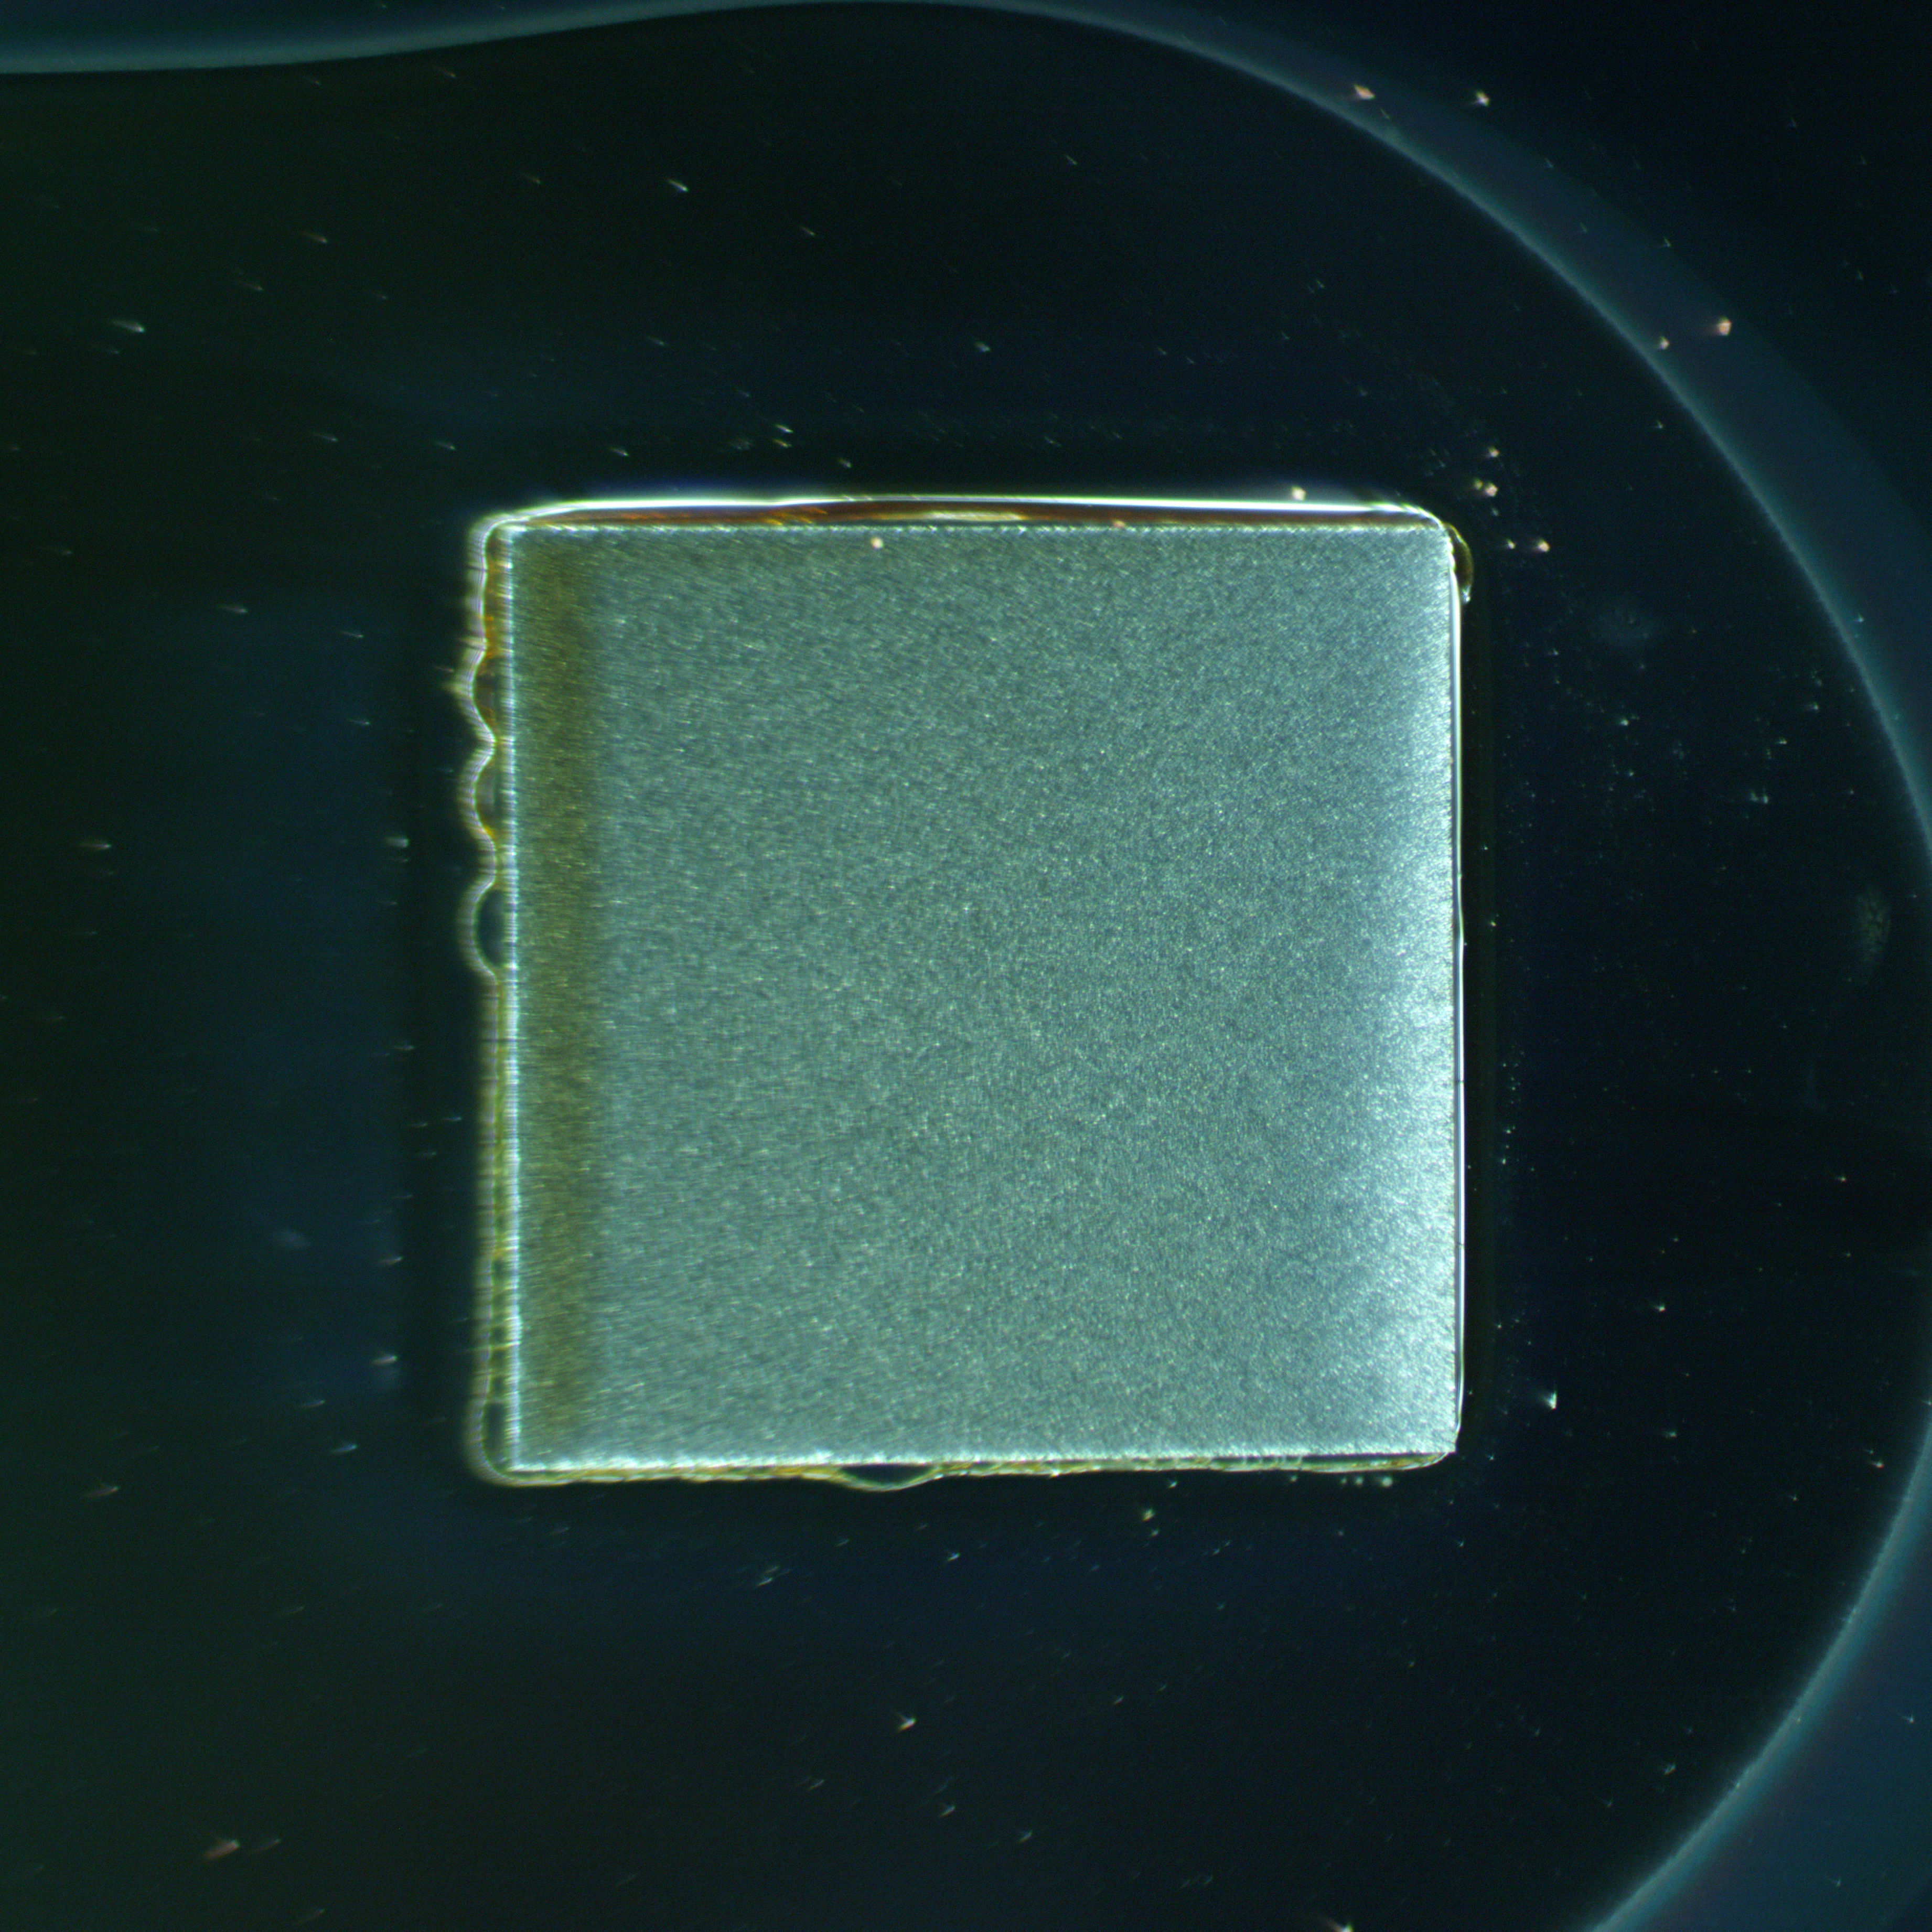
\includegraphics[width=\linewidth]{pics/spincoat/no6/6101.jpg}
        \caption{Heater 1}
    \end{subfigure}
    \hfill
    \begin{subfigure}[t]{0.3\textwidth}
        \centering
        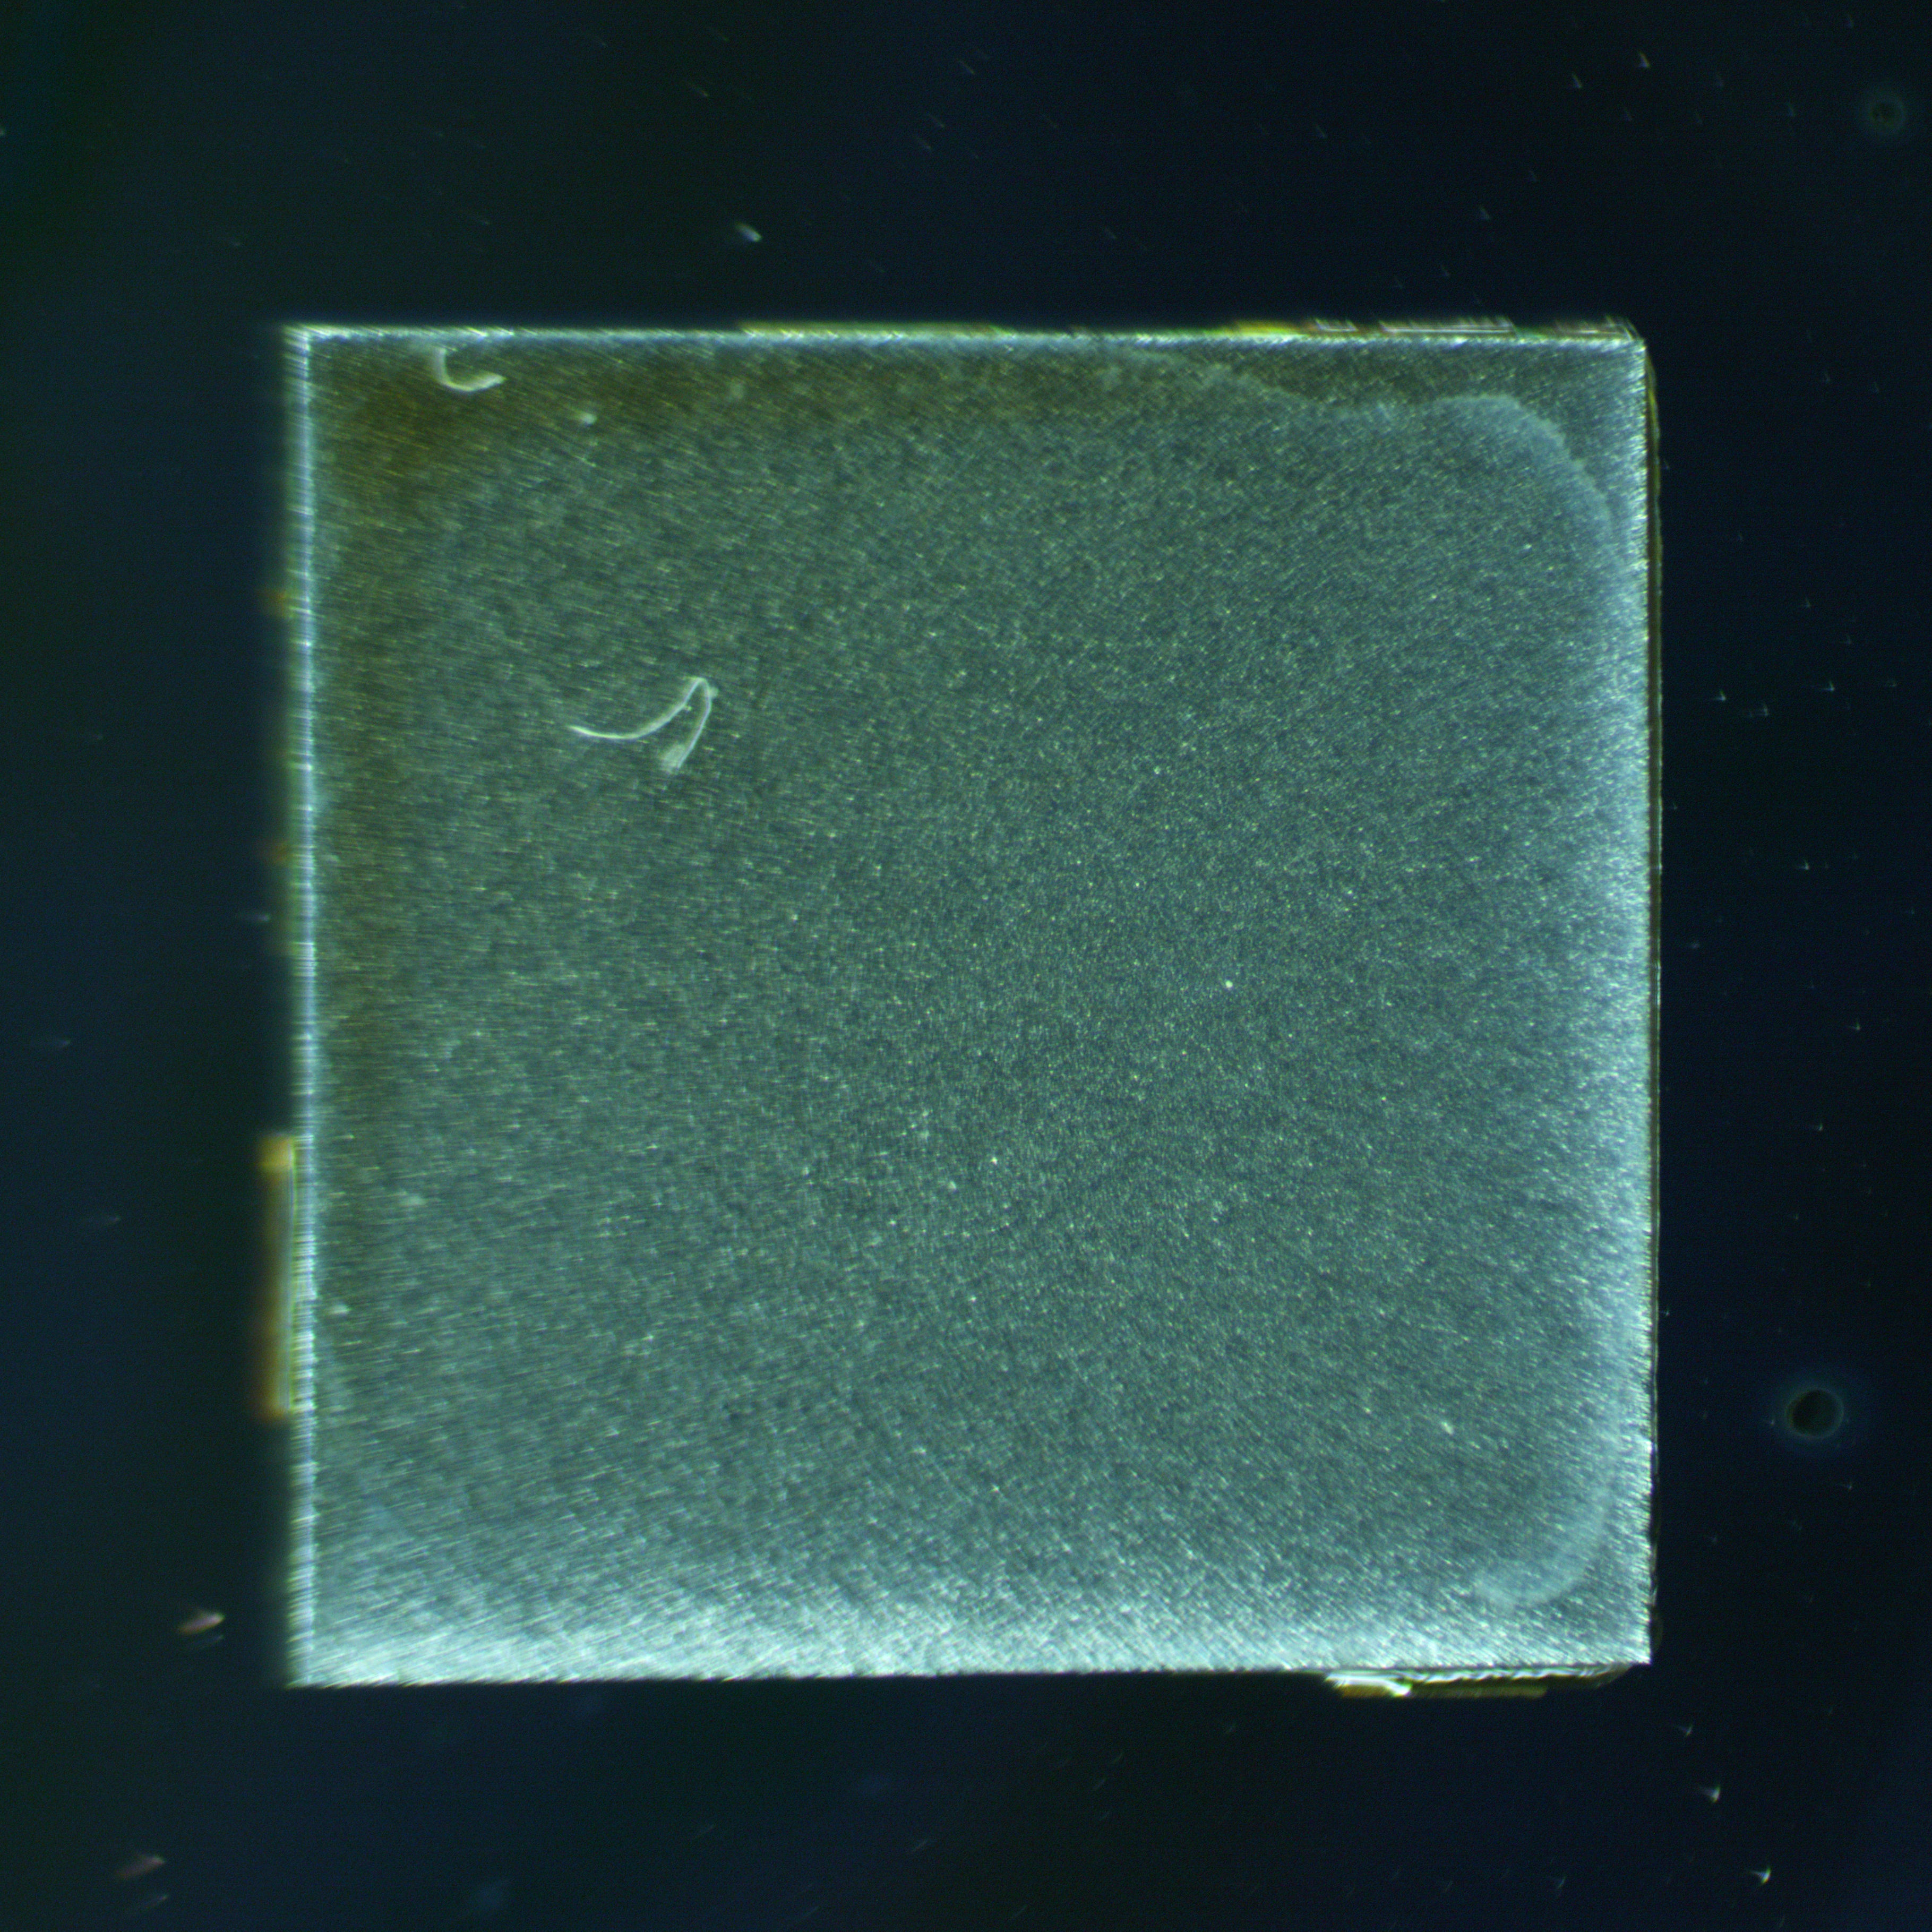
\includegraphics[width=\linewidth]{pics/spincoat/no6/6110.jpg}
        \caption{\textcolor{blue!60!black}{\textbf{Heater 2}}}
    \end{subfigure}
    \hfill
    \begin{subfigure}[t]{0.3\textwidth}
        \centering
        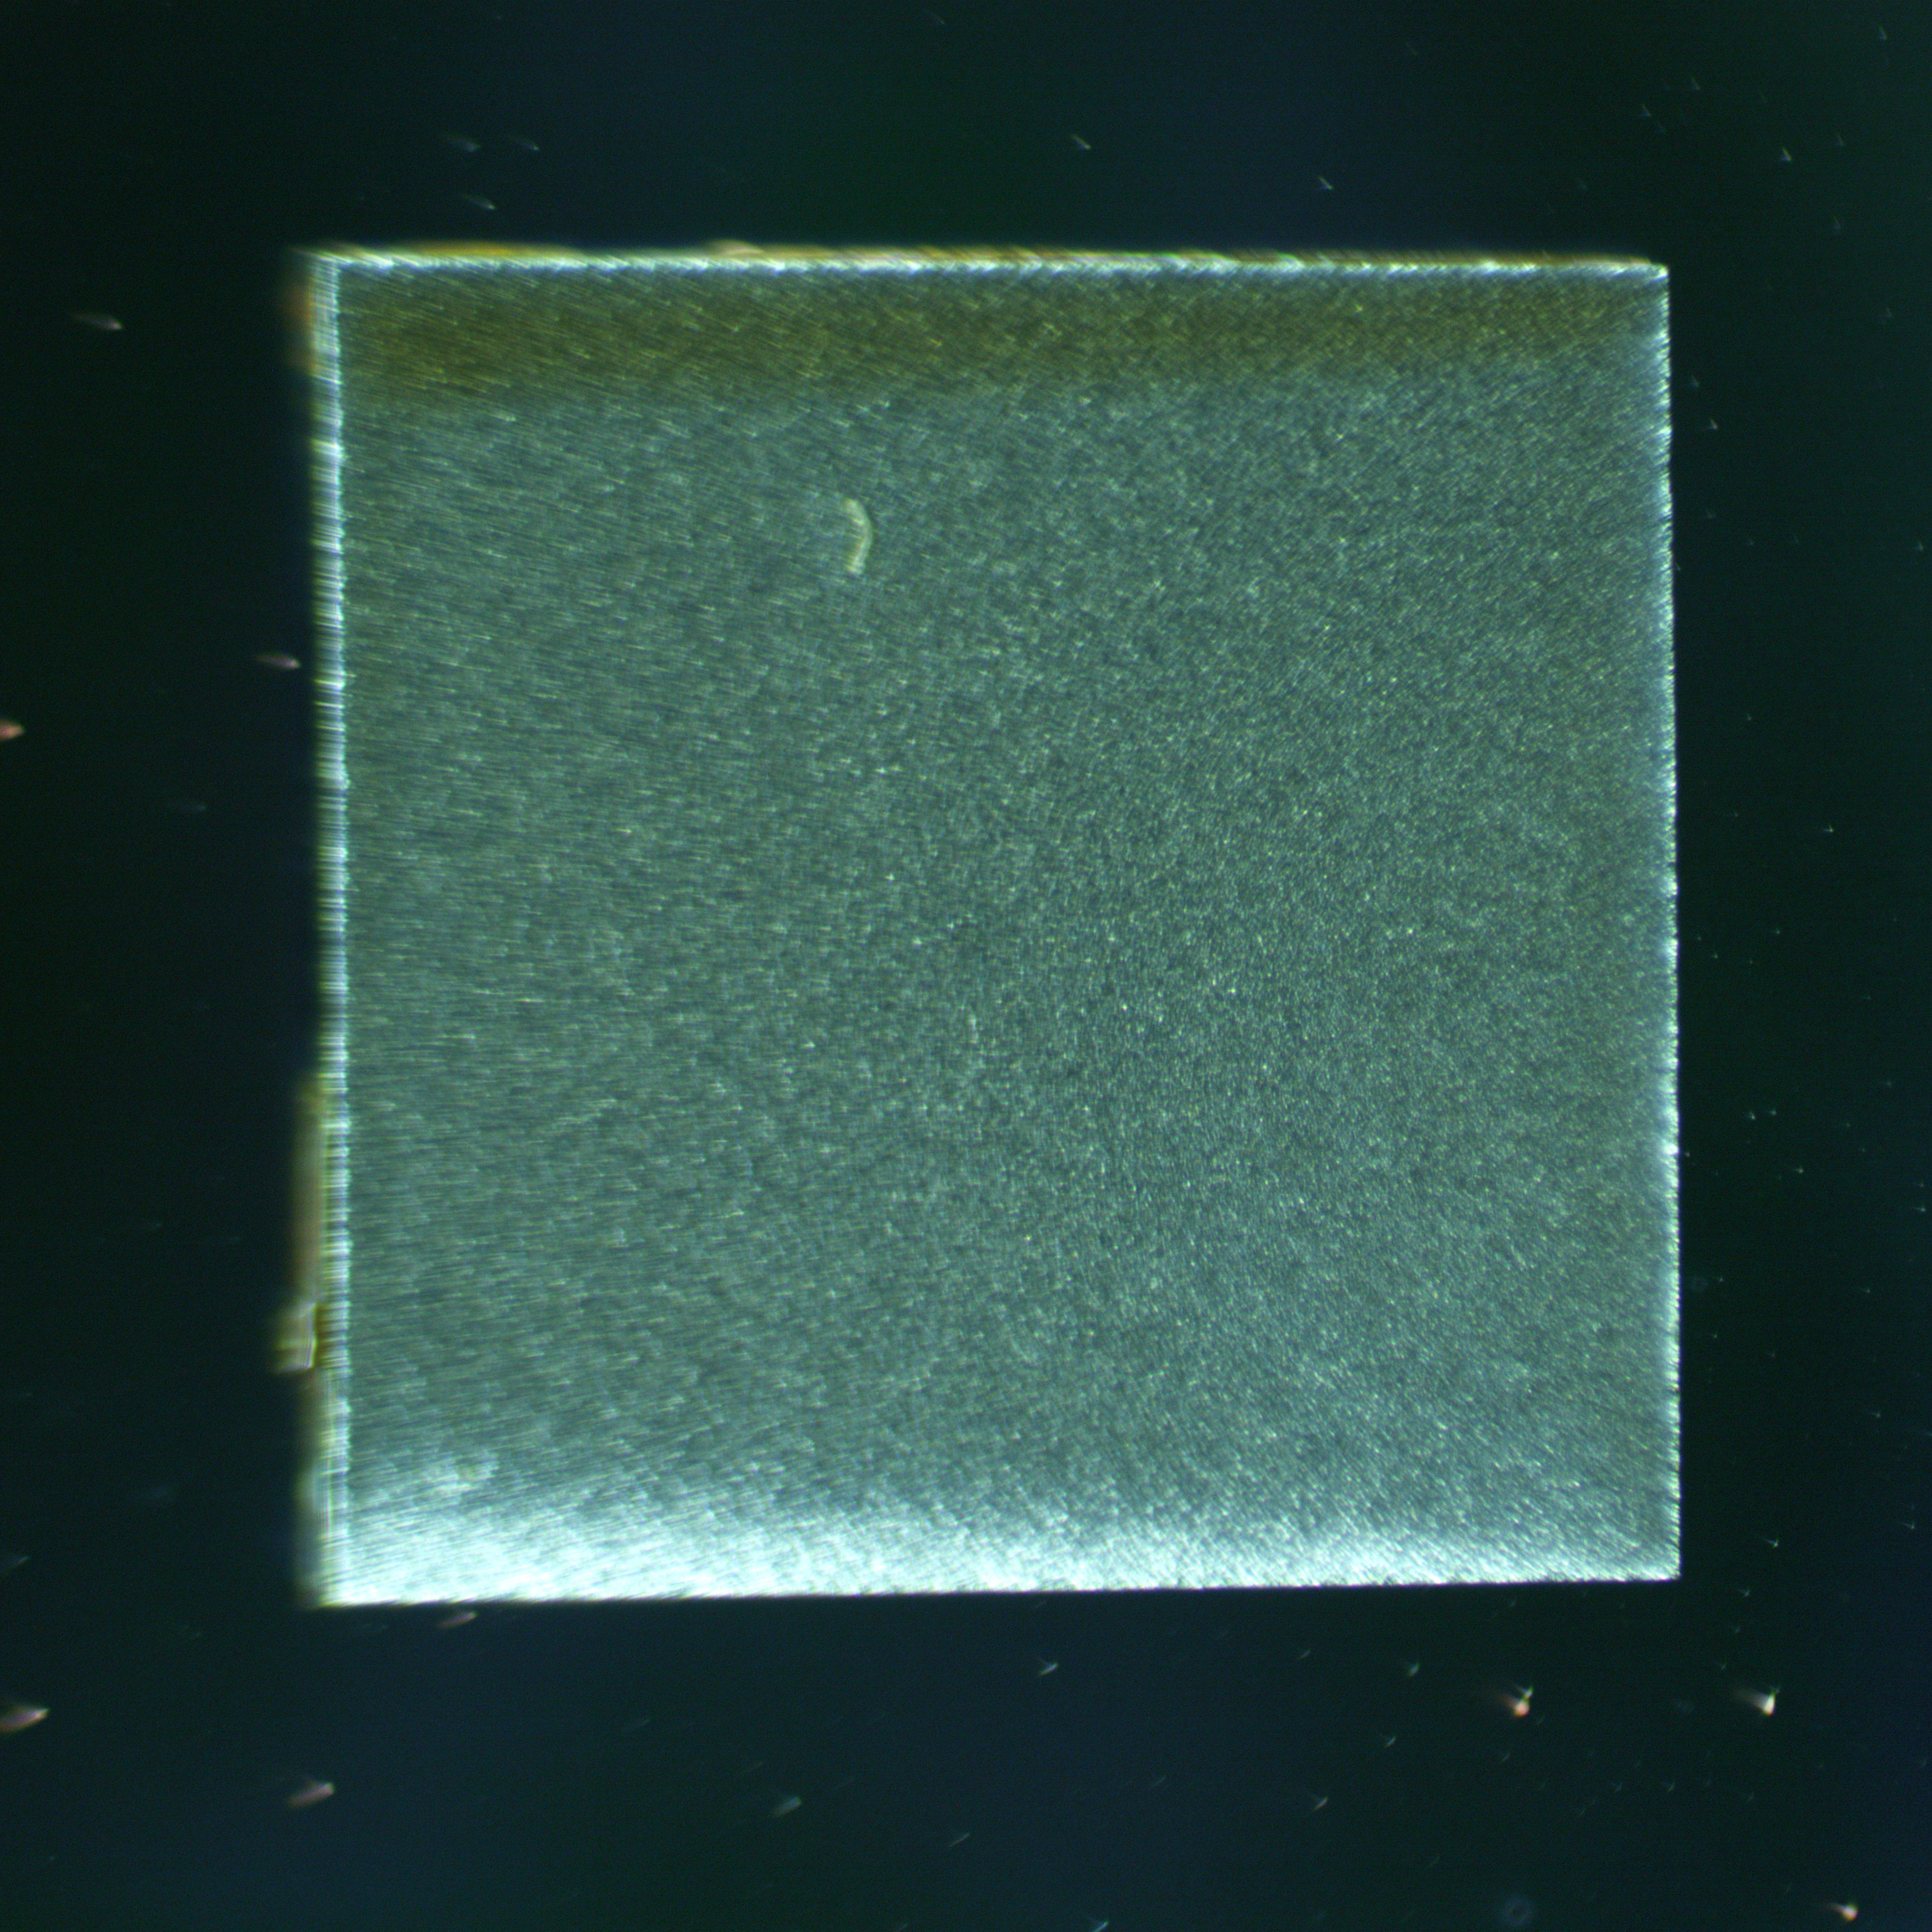
\includegraphics[width=\linewidth]{pics/spincoat/no6/6111.jpg}
        \caption{\textcolor{blue!60!black}{\textbf{Heater 3}}}
    \end{subfigure}

    \vspace{0.8cm}

    % ---------- Row 2 ----------
    \begin{subfigure}[t]{0.3\textwidth}
        \centering
        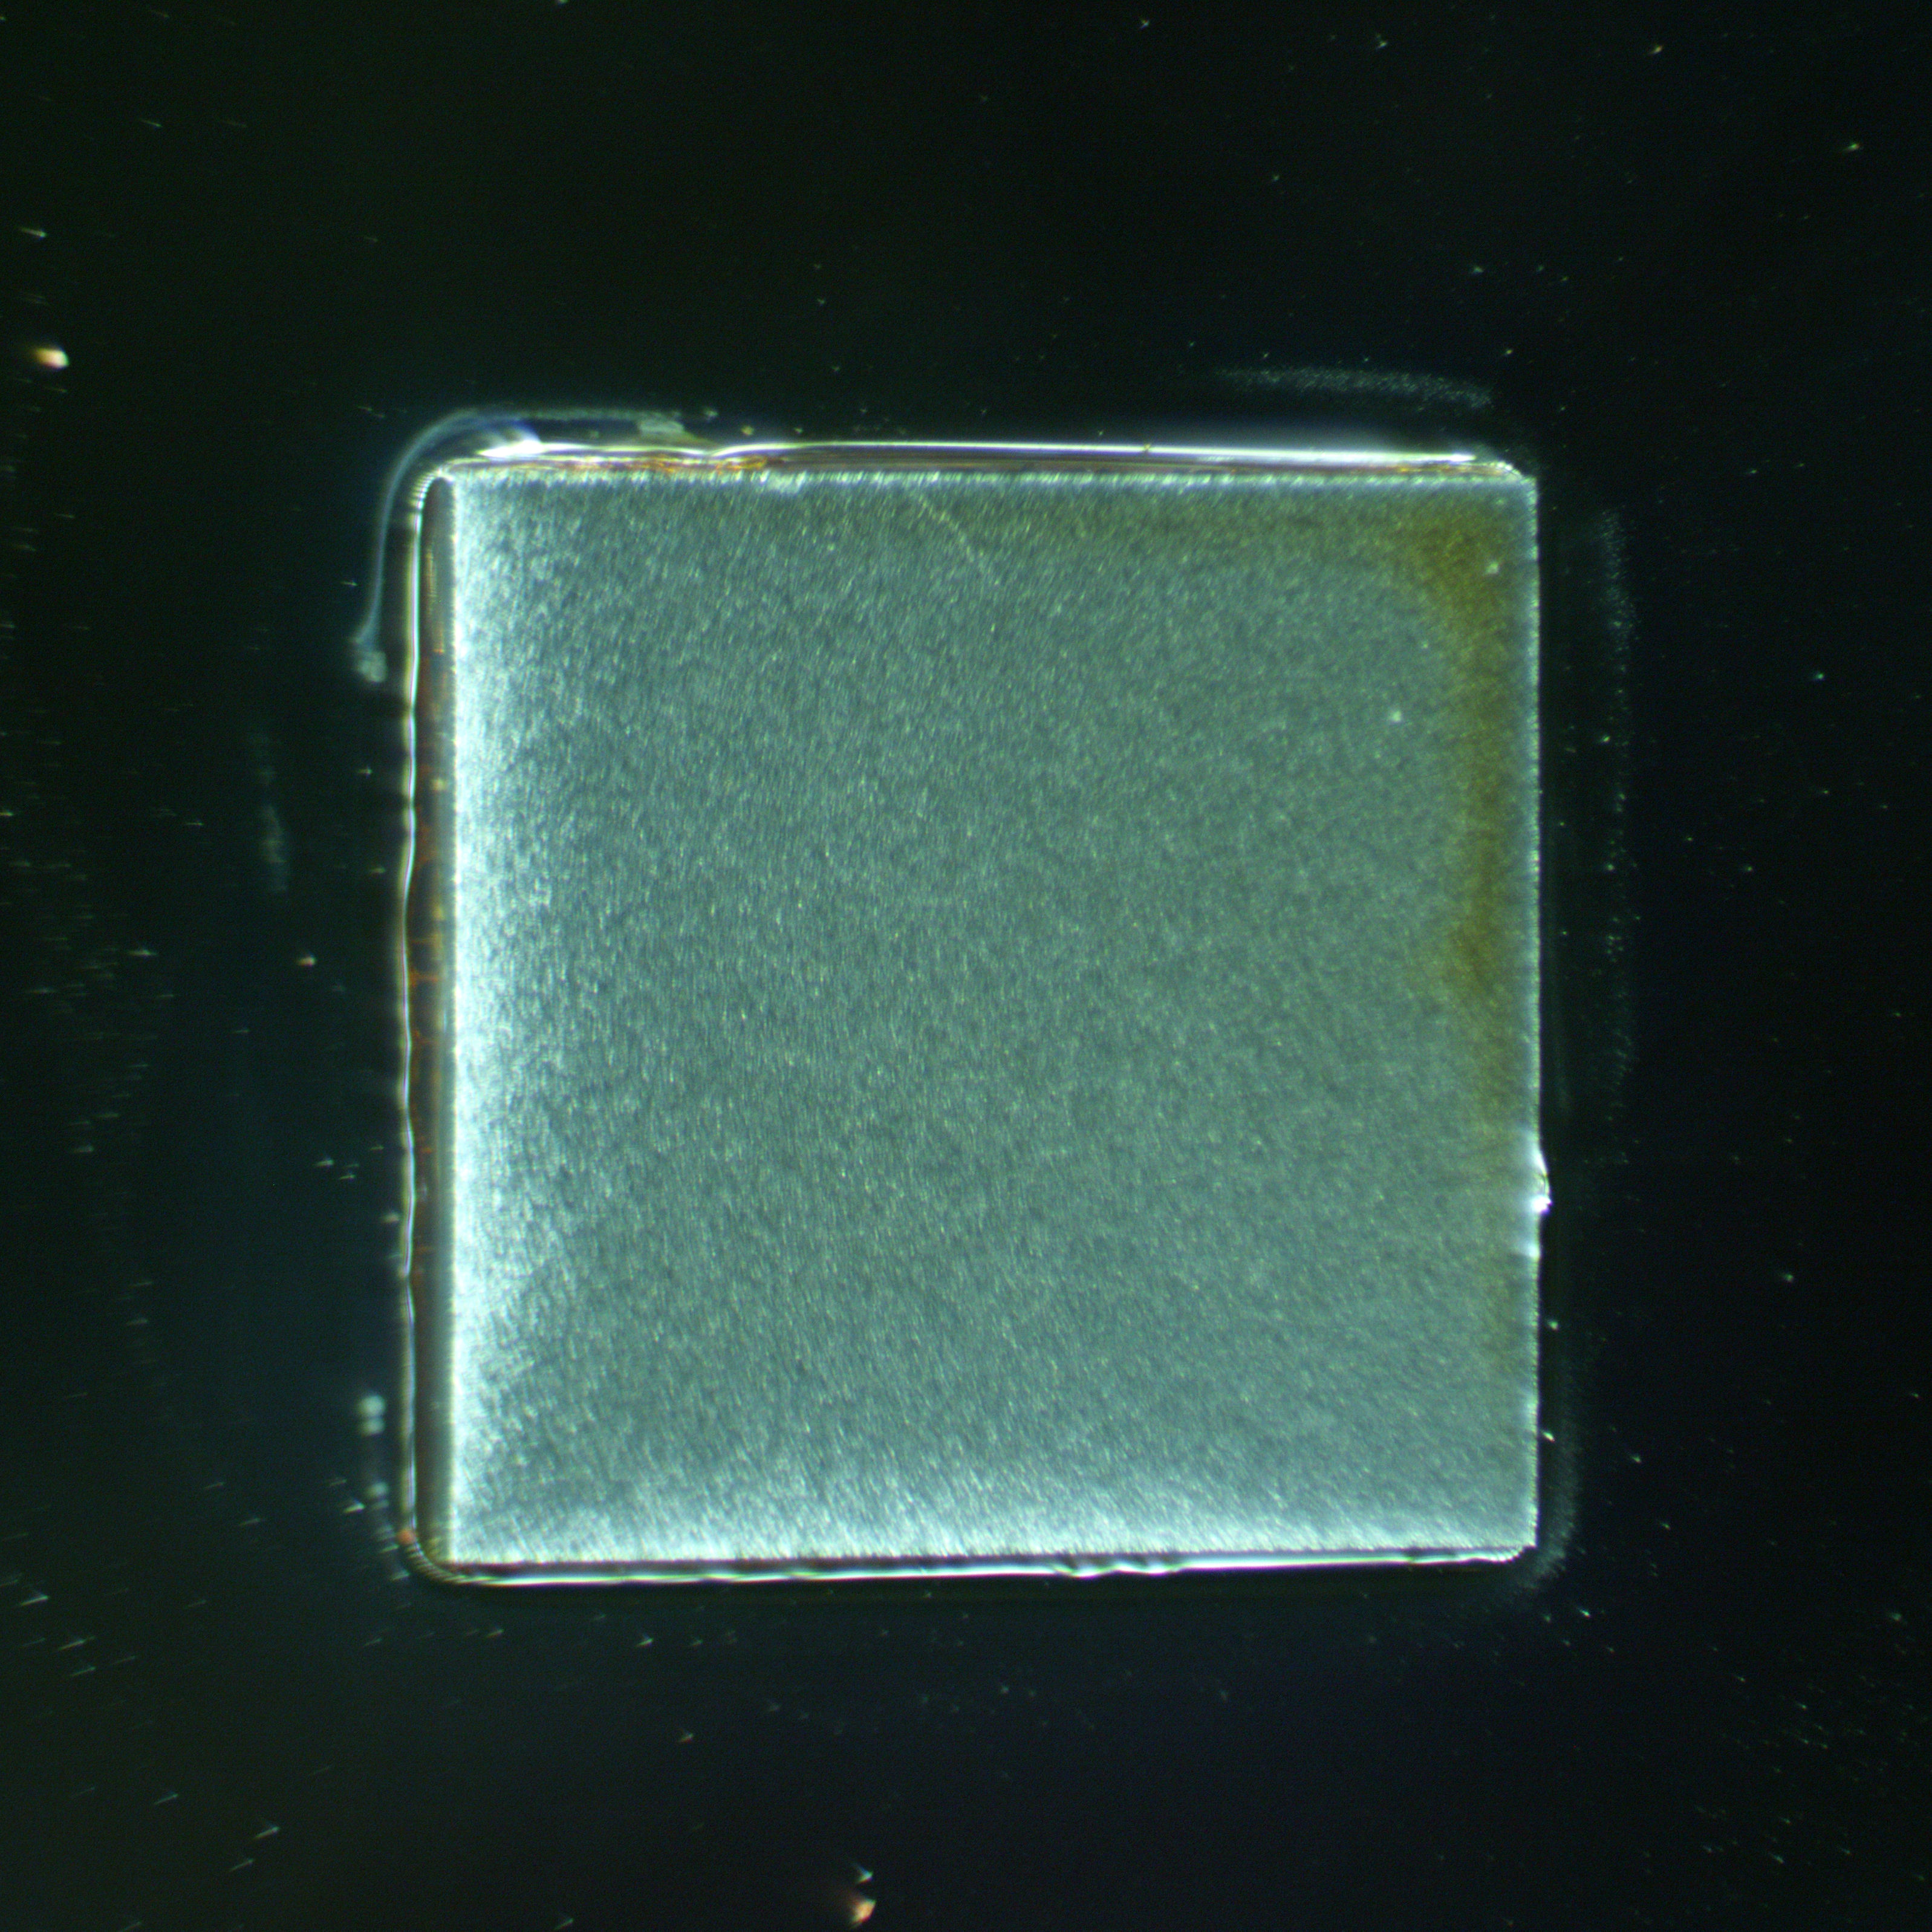
\includegraphics[width=\linewidth]{pics/spincoat/no6/6104.jpg}
        \caption{Heater 4}
    \end{subfigure}
    \hfill
    \begin{subfigure}[t]{0.3\textwidth}
        \centering
        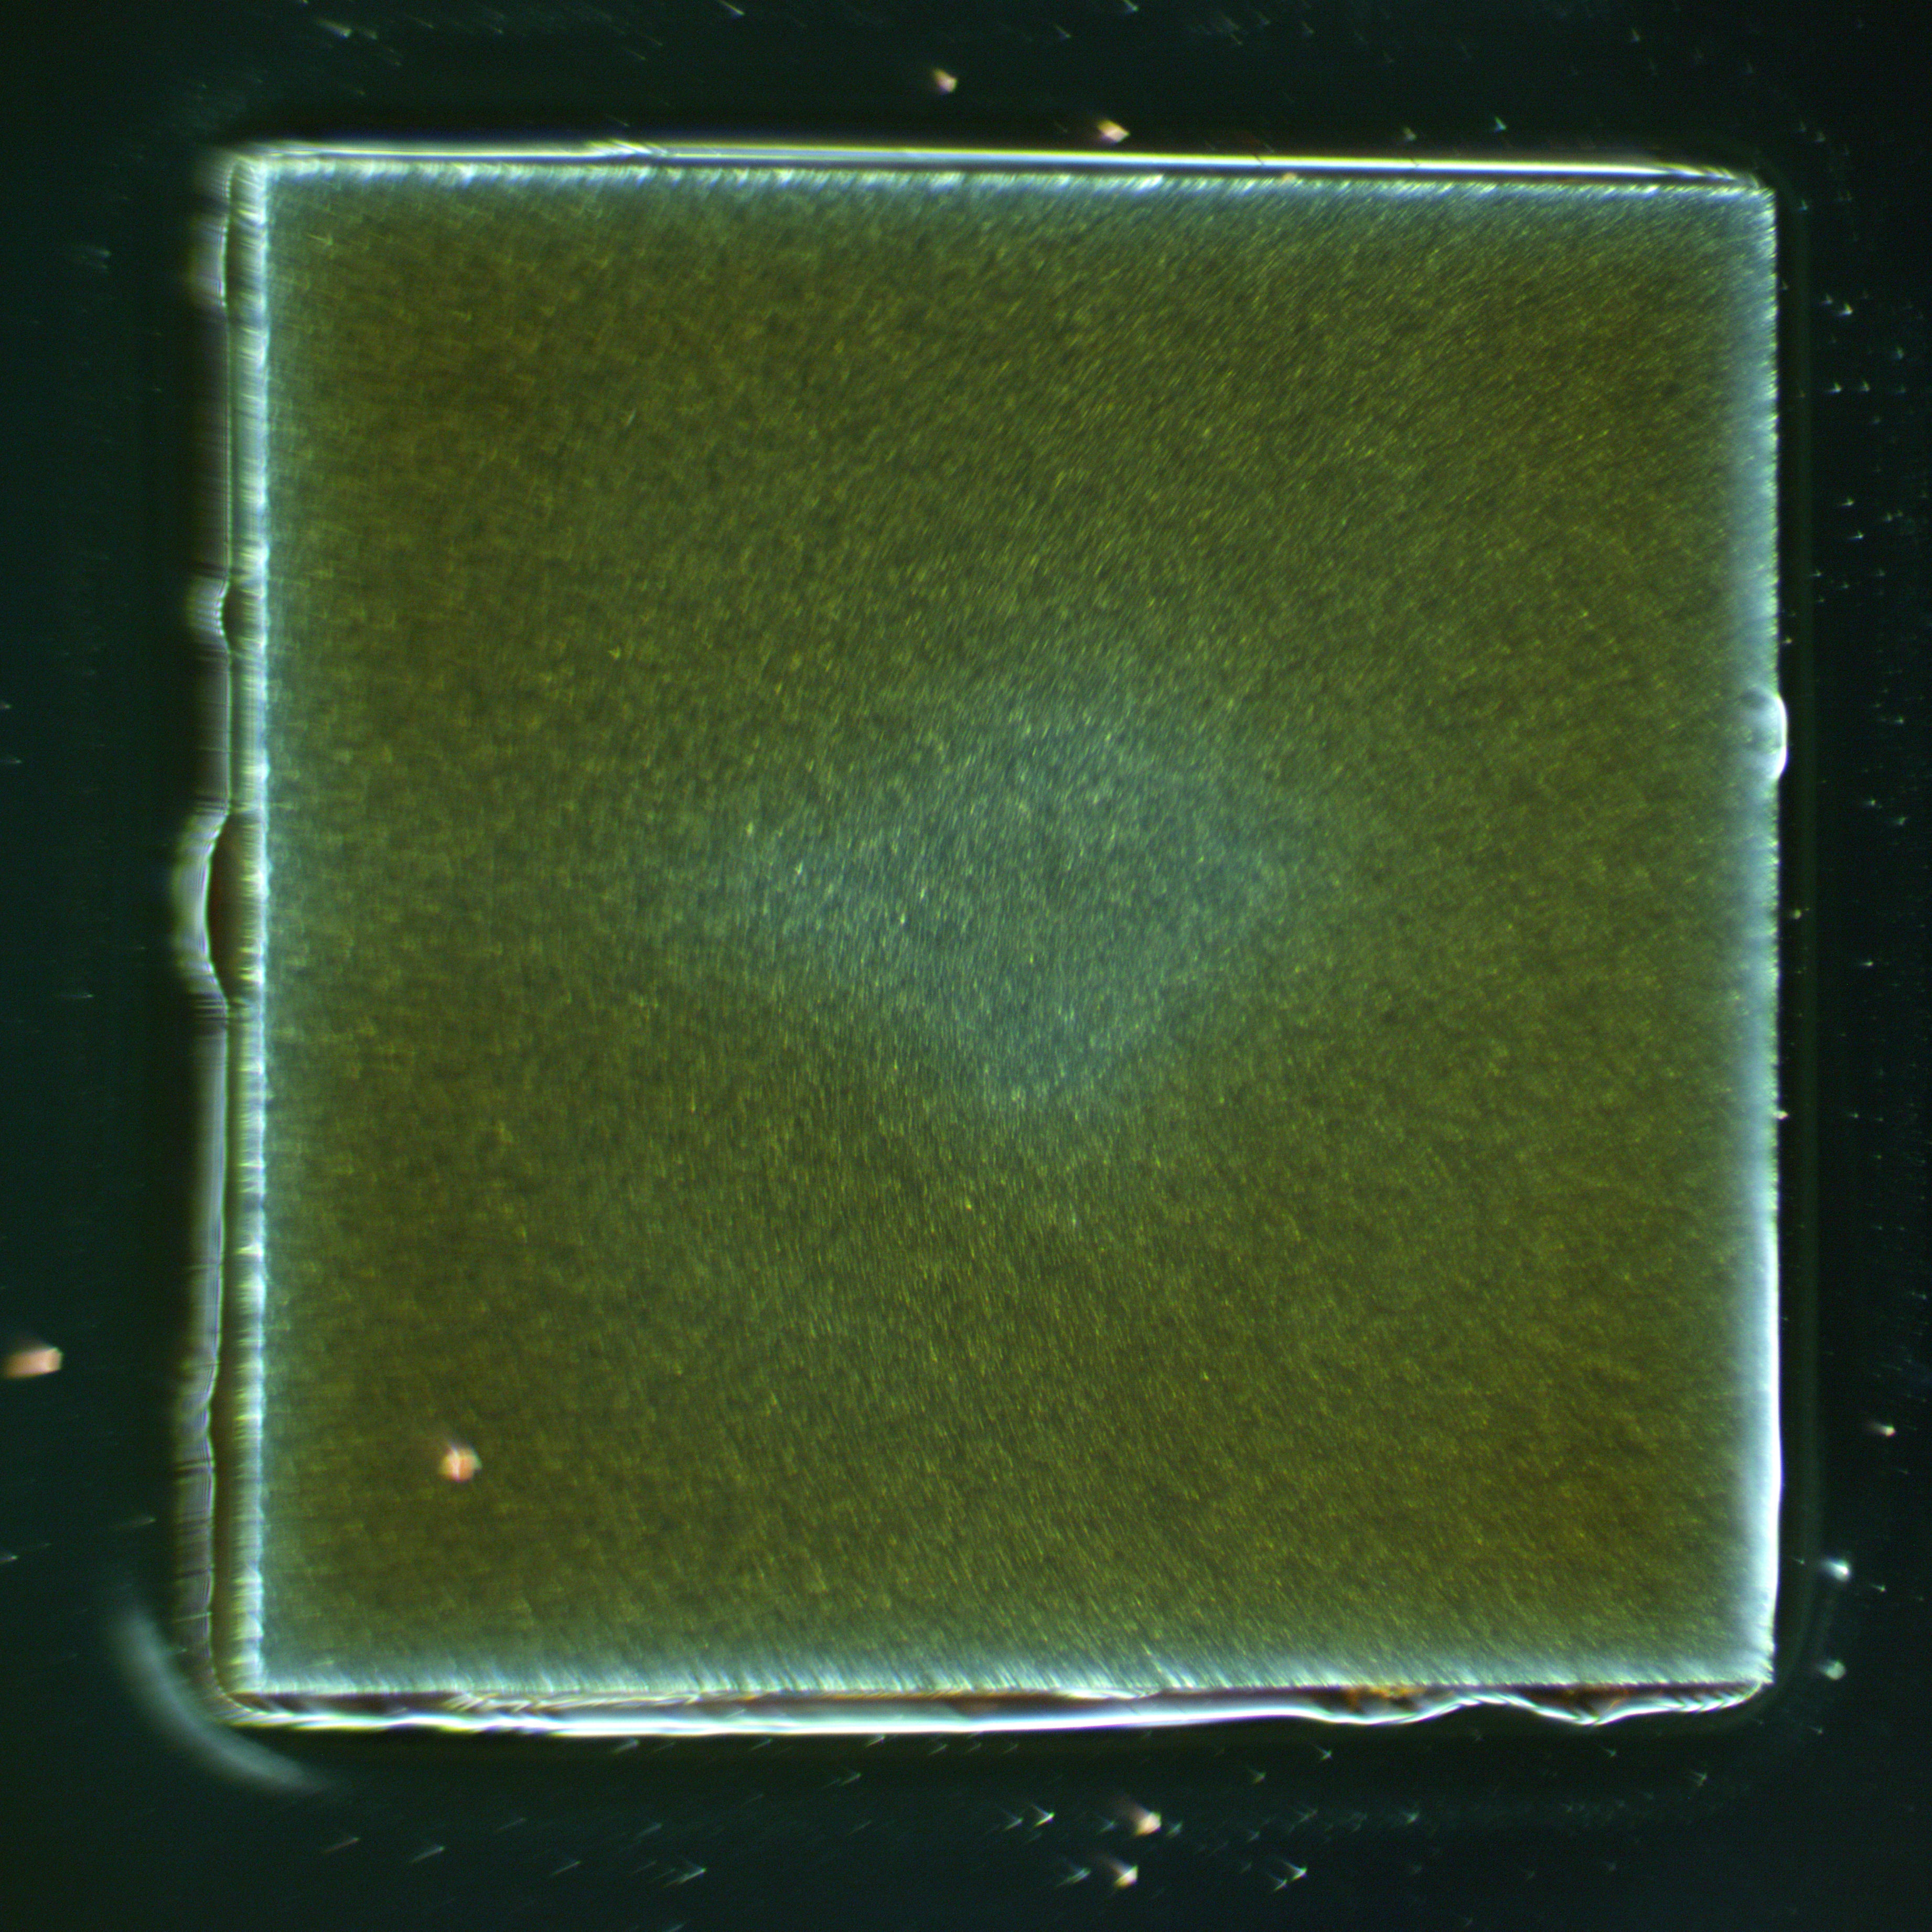
\includegraphics[width=\linewidth]{pics/spincoat/no6/6105.jpg}
        \caption{Heater 5}
    \end{subfigure}
    \hfill
    \begin{subfigure}[t]{0.3\textwidth}
        \centering
        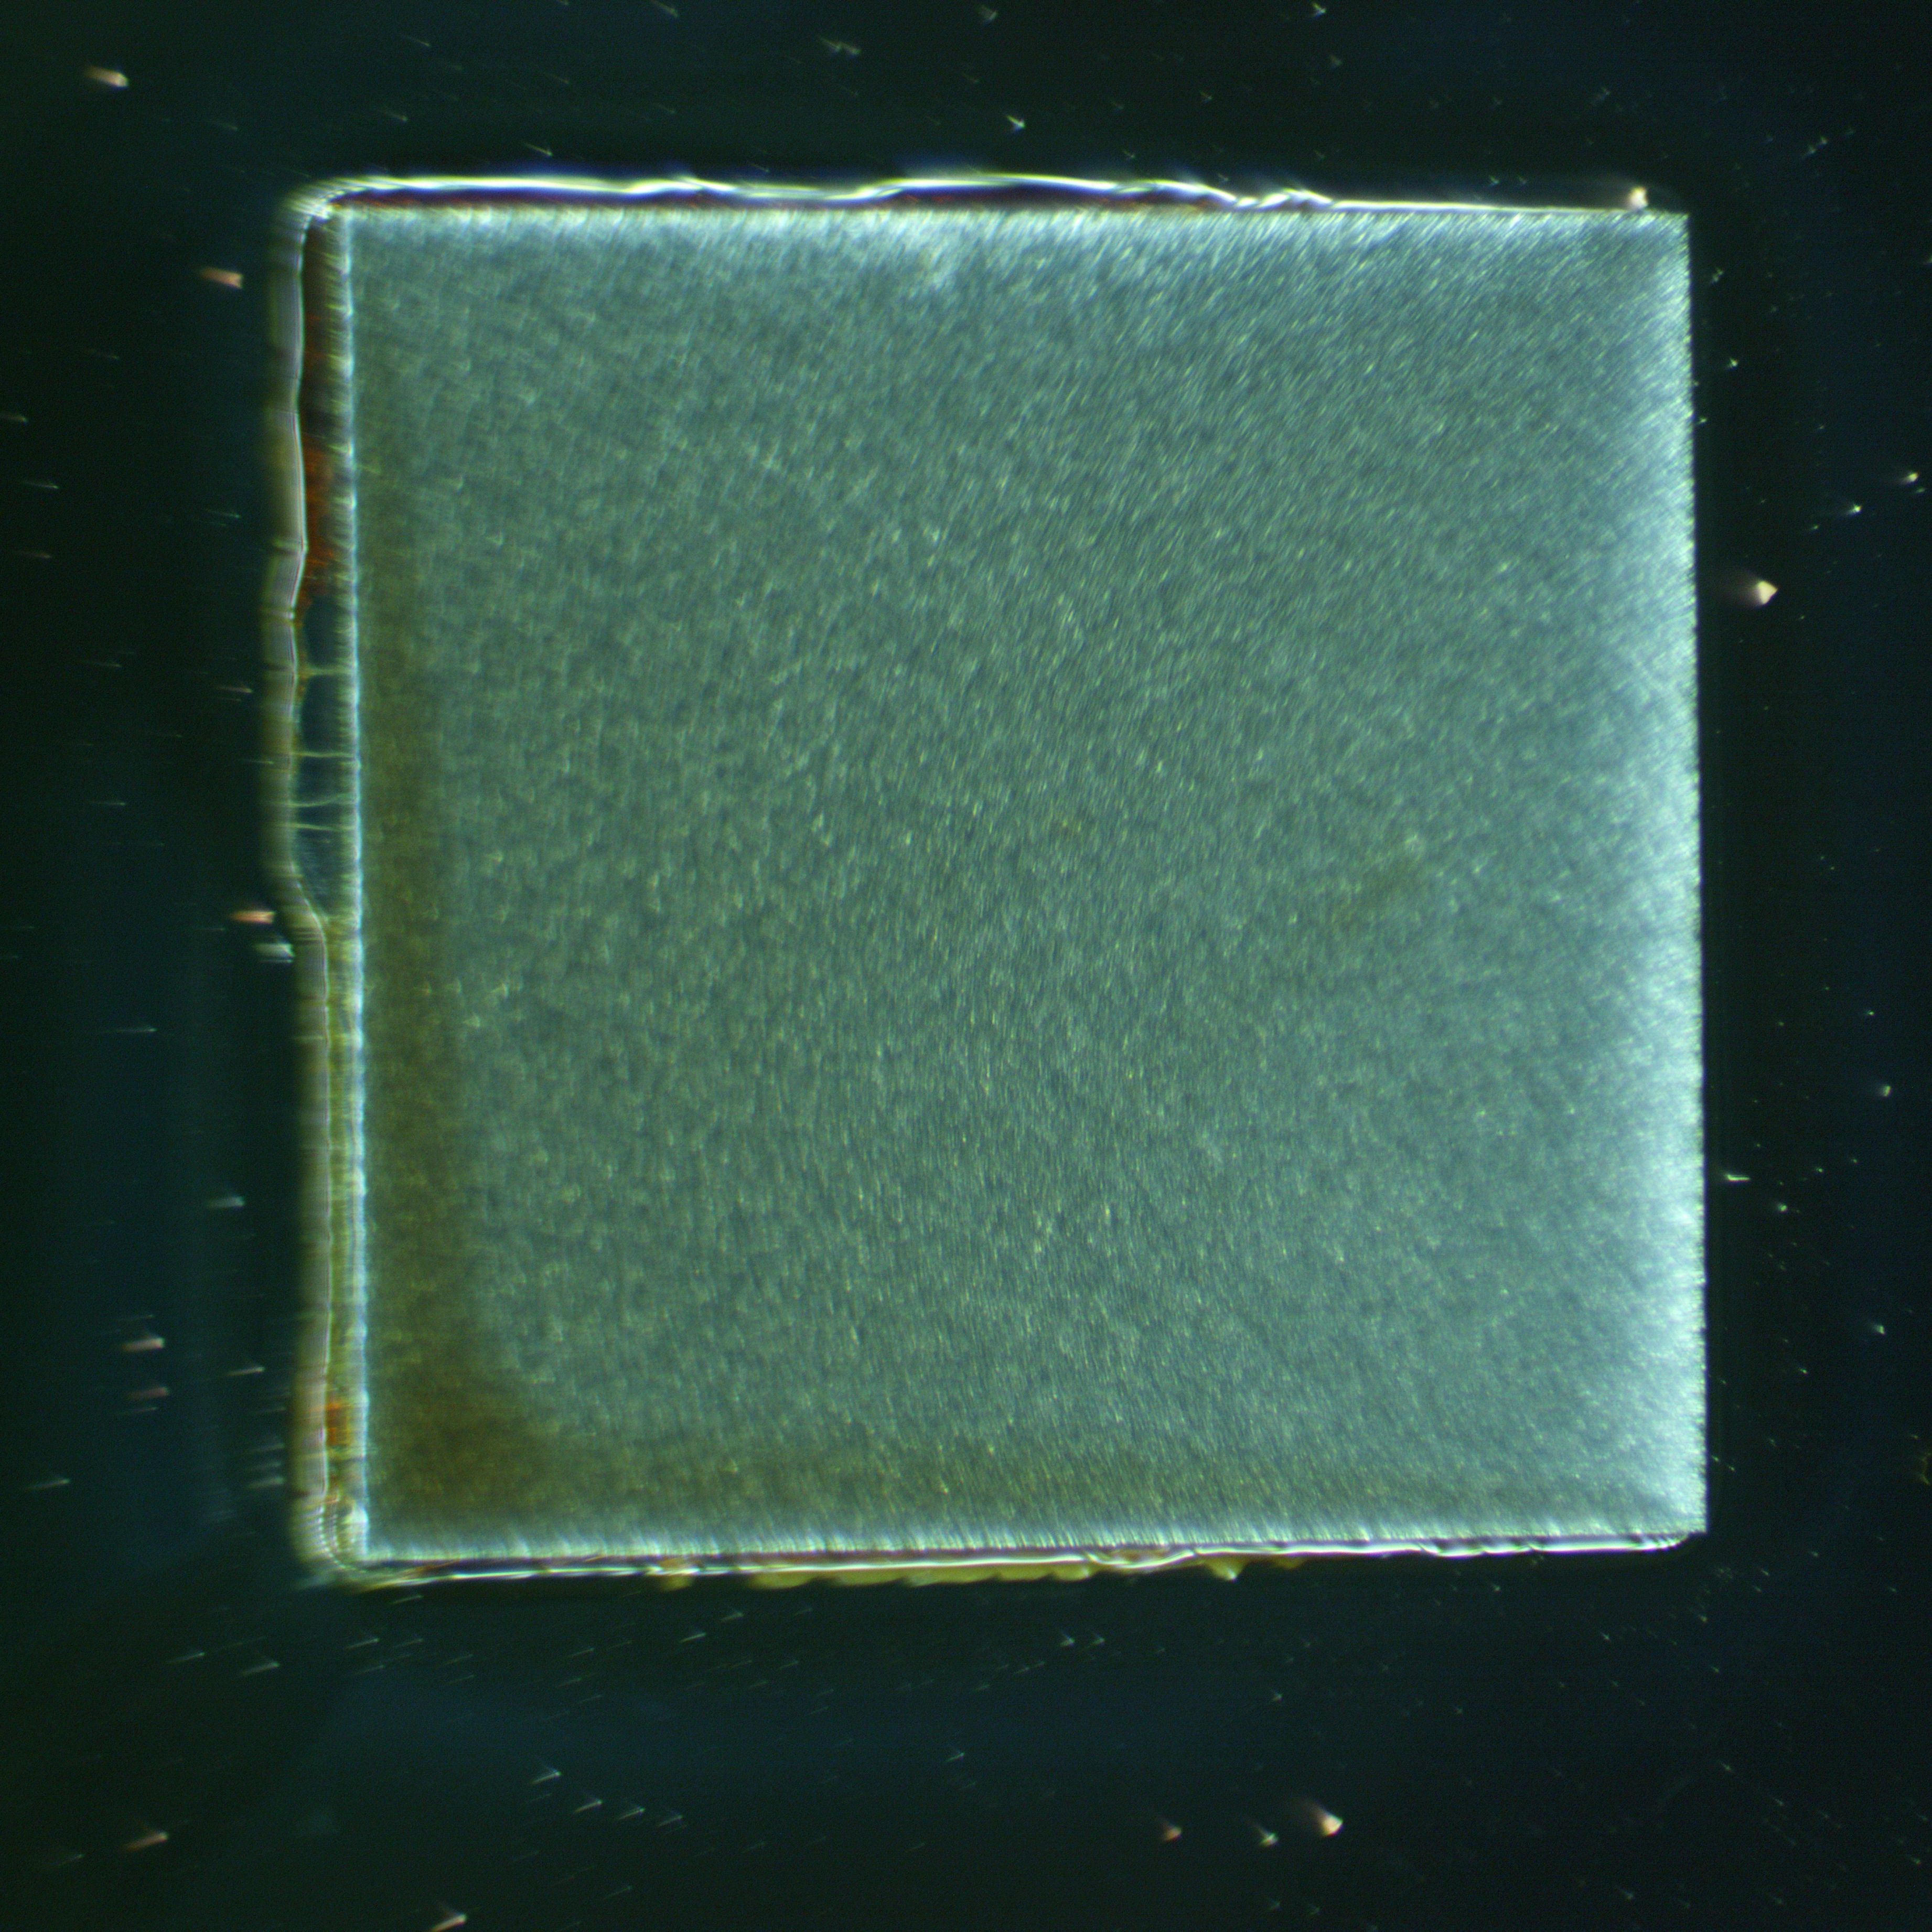
\includegraphics[width=\linewidth]{pics/spincoat/no6/6106.jpg}
        \caption{Heater 6}
    \end{subfigure}

    \vspace{0.8cm}

    % ---------- Row 3 ----------
    \begin{subfigure}[t]{0.3\textwidth}
        \centering
        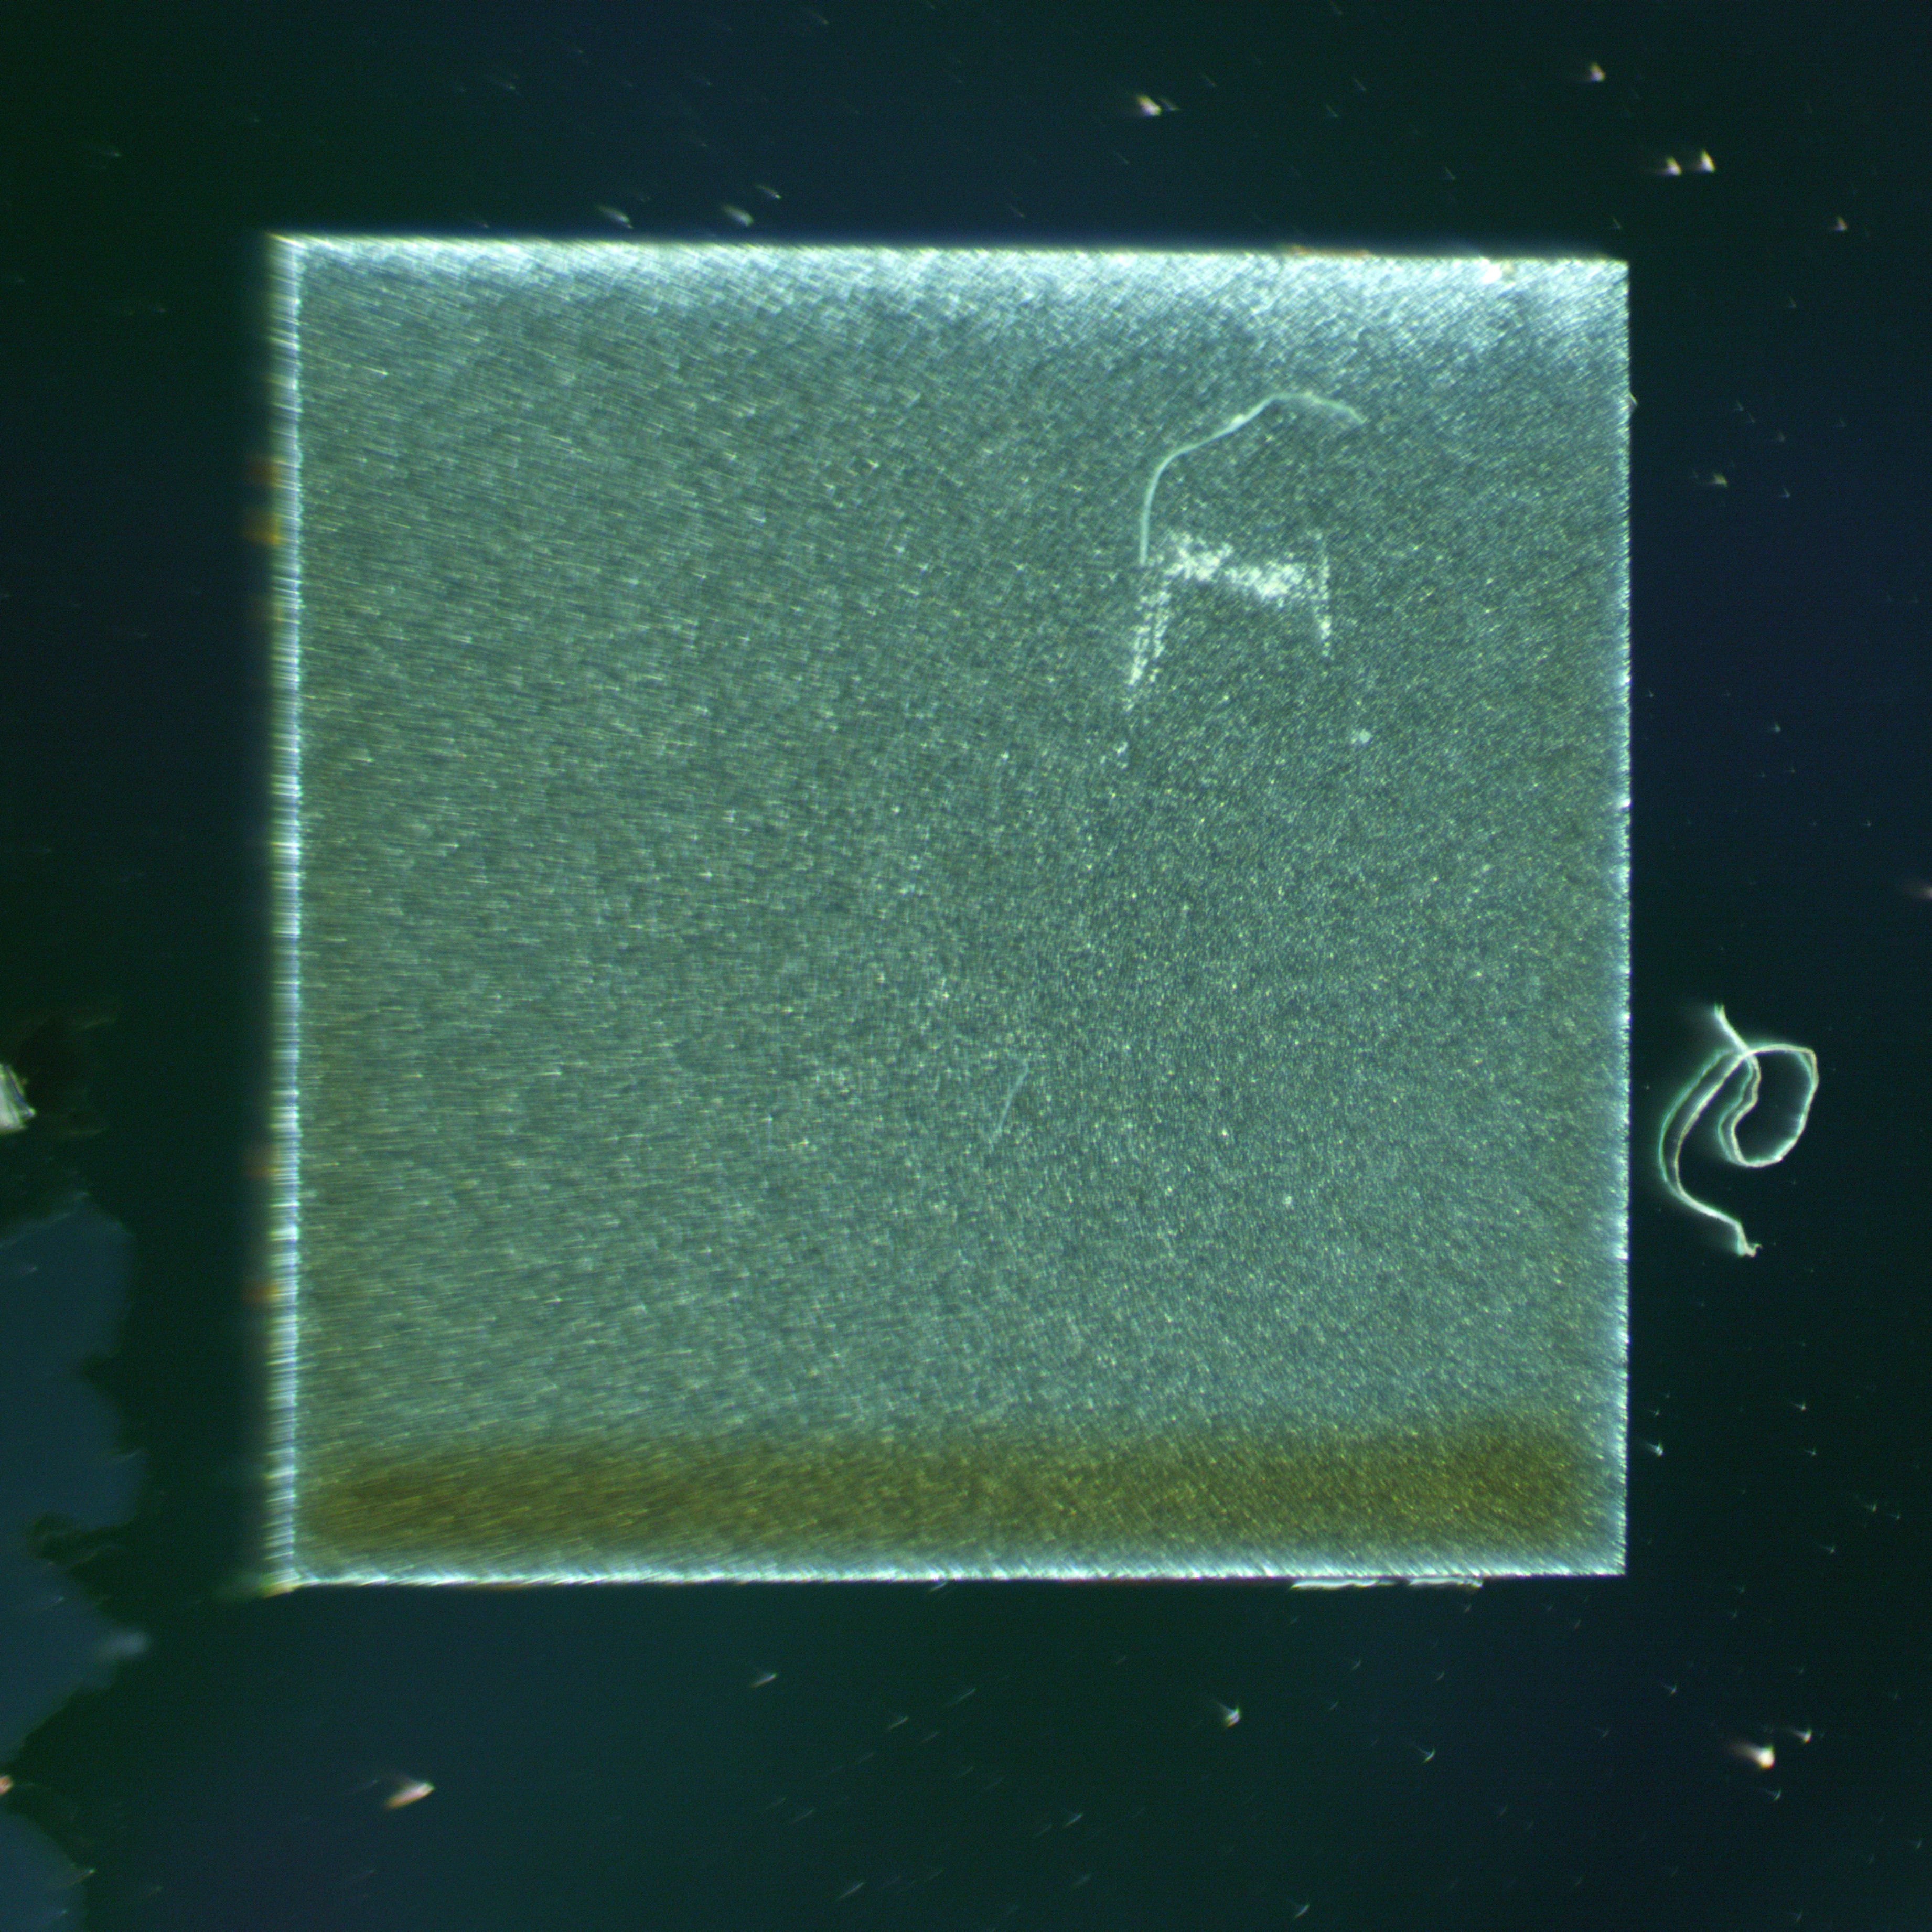
\includegraphics[width=\linewidth]{pics/spincoat/no6/6112.jpg}
        \caption{\textcolor{blue!60!black}{\textbf{Heater 7}}}
    \end{subfigure}
    \hfill
    \begin{subfigure}[t]{0.3\textwidth}
        \centering
        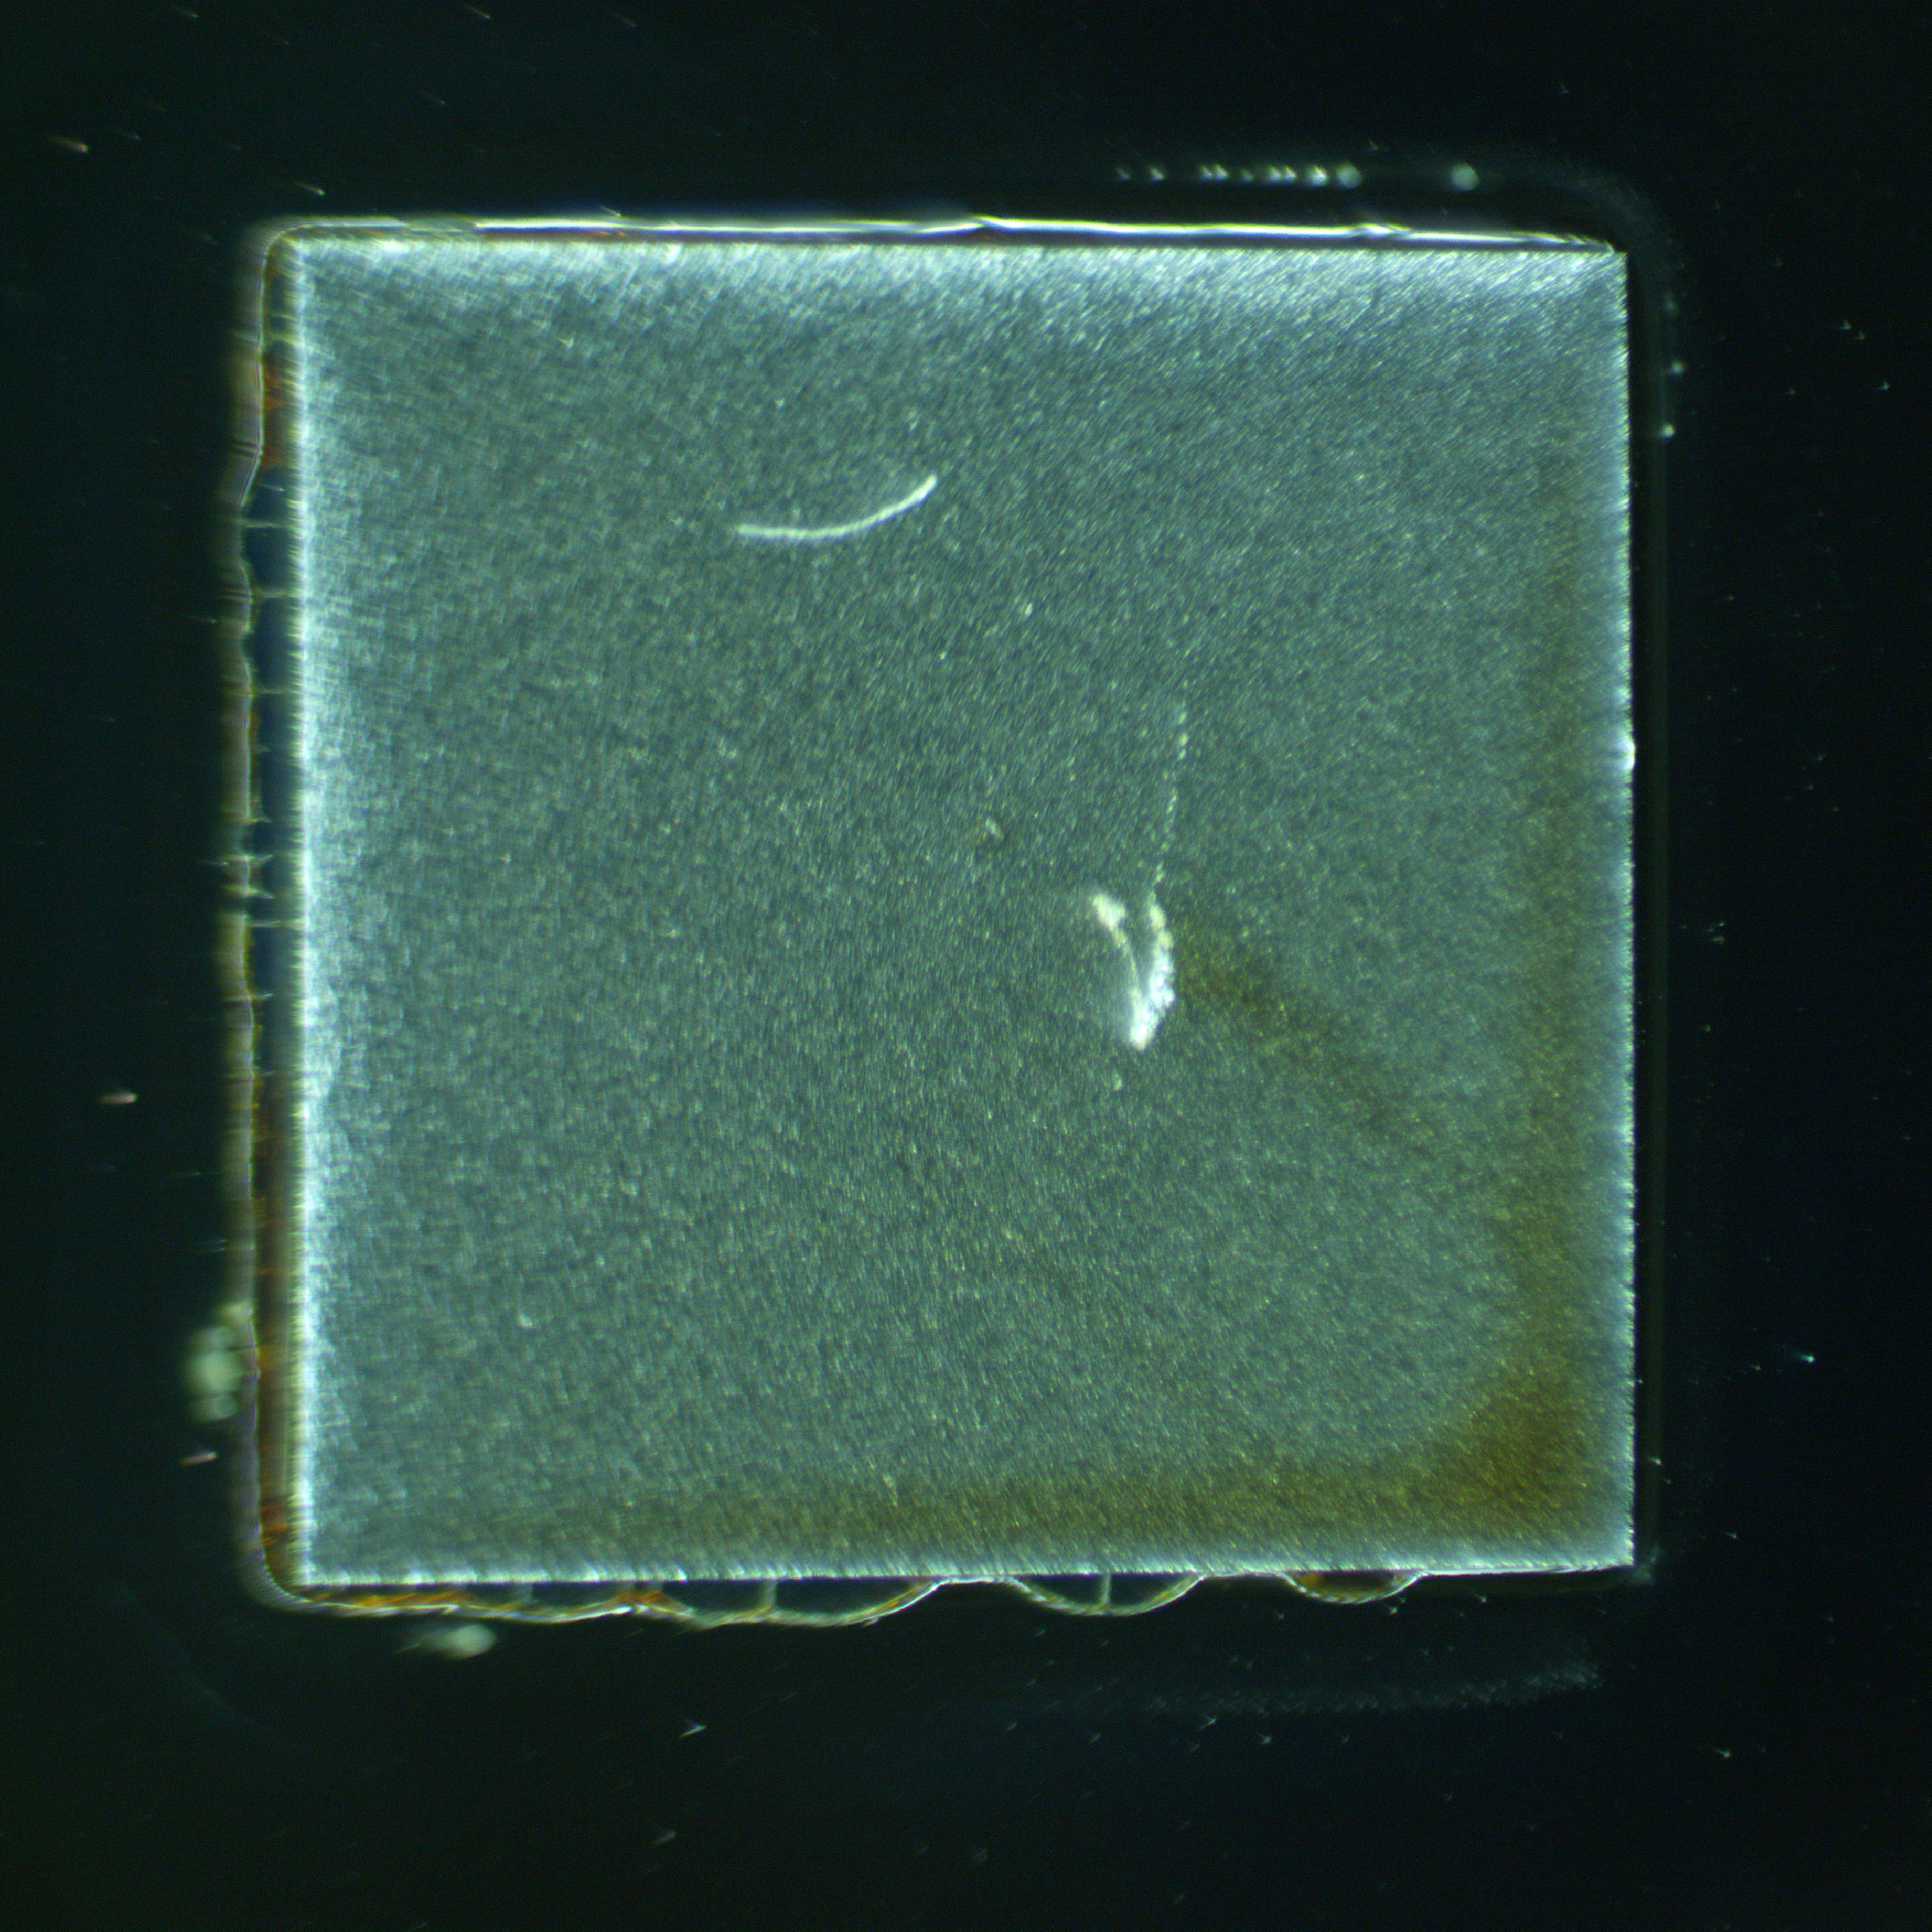
\includegraphics[width=\linewidth]{pics/spincoat/no6/6108.jpg}
        \caption{Heater 8}
    \end{subfigure}
    \hfill
    \begin{subfigure}[t]{0.3\textwidth}
        \centering
        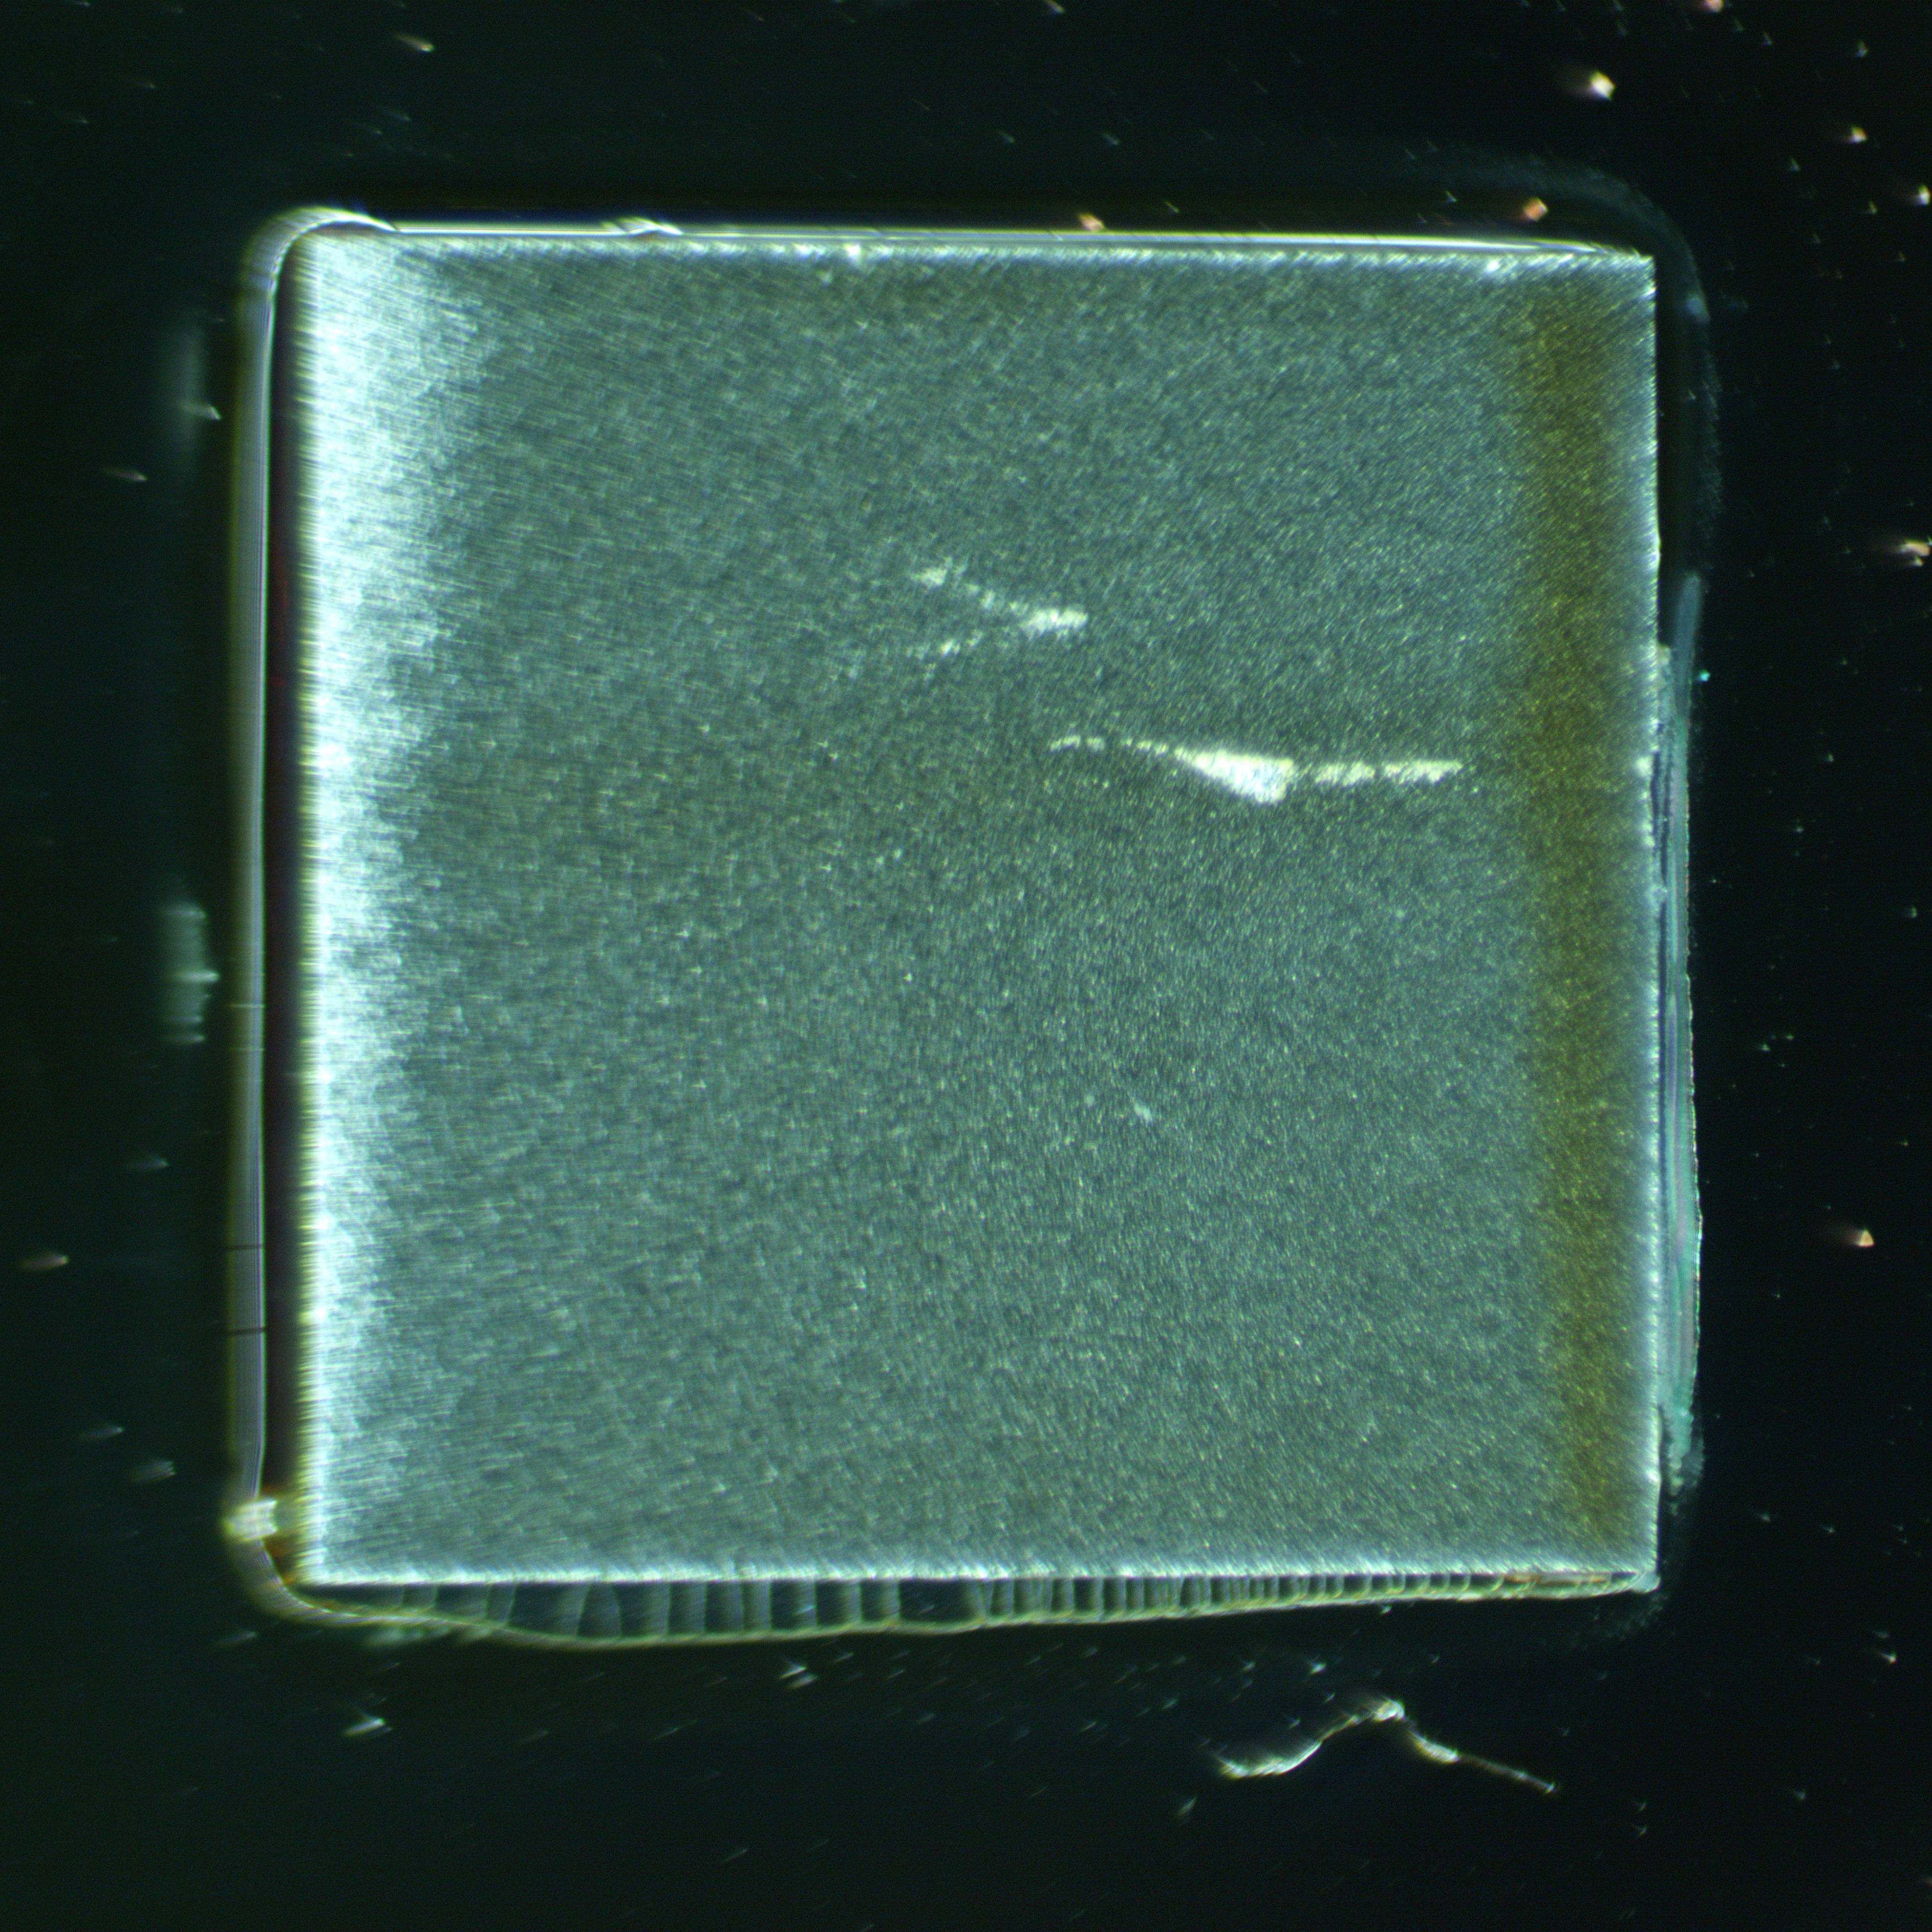
\includegraphics[width=\linewidth]{pics/spincoat/no6/6109.jpg}
        \caption{Heater 9}
    \end{subfigure}

    \caption[Optical Images of the Heater in Passivation Test \#6]{Optical images of the nine Heater of the coating test \#6. The two heaters that could be removed from the glue are highlighted in blue.}
    \label{fig:PT6}
\end{figure}
%================================================================================
%================================================================================
\begin{figure}[htbp]
    \centering

    % ---------- Row 1 ----------
    \begin{subfigure}[t]{0.3\textwidth}
        \centering
        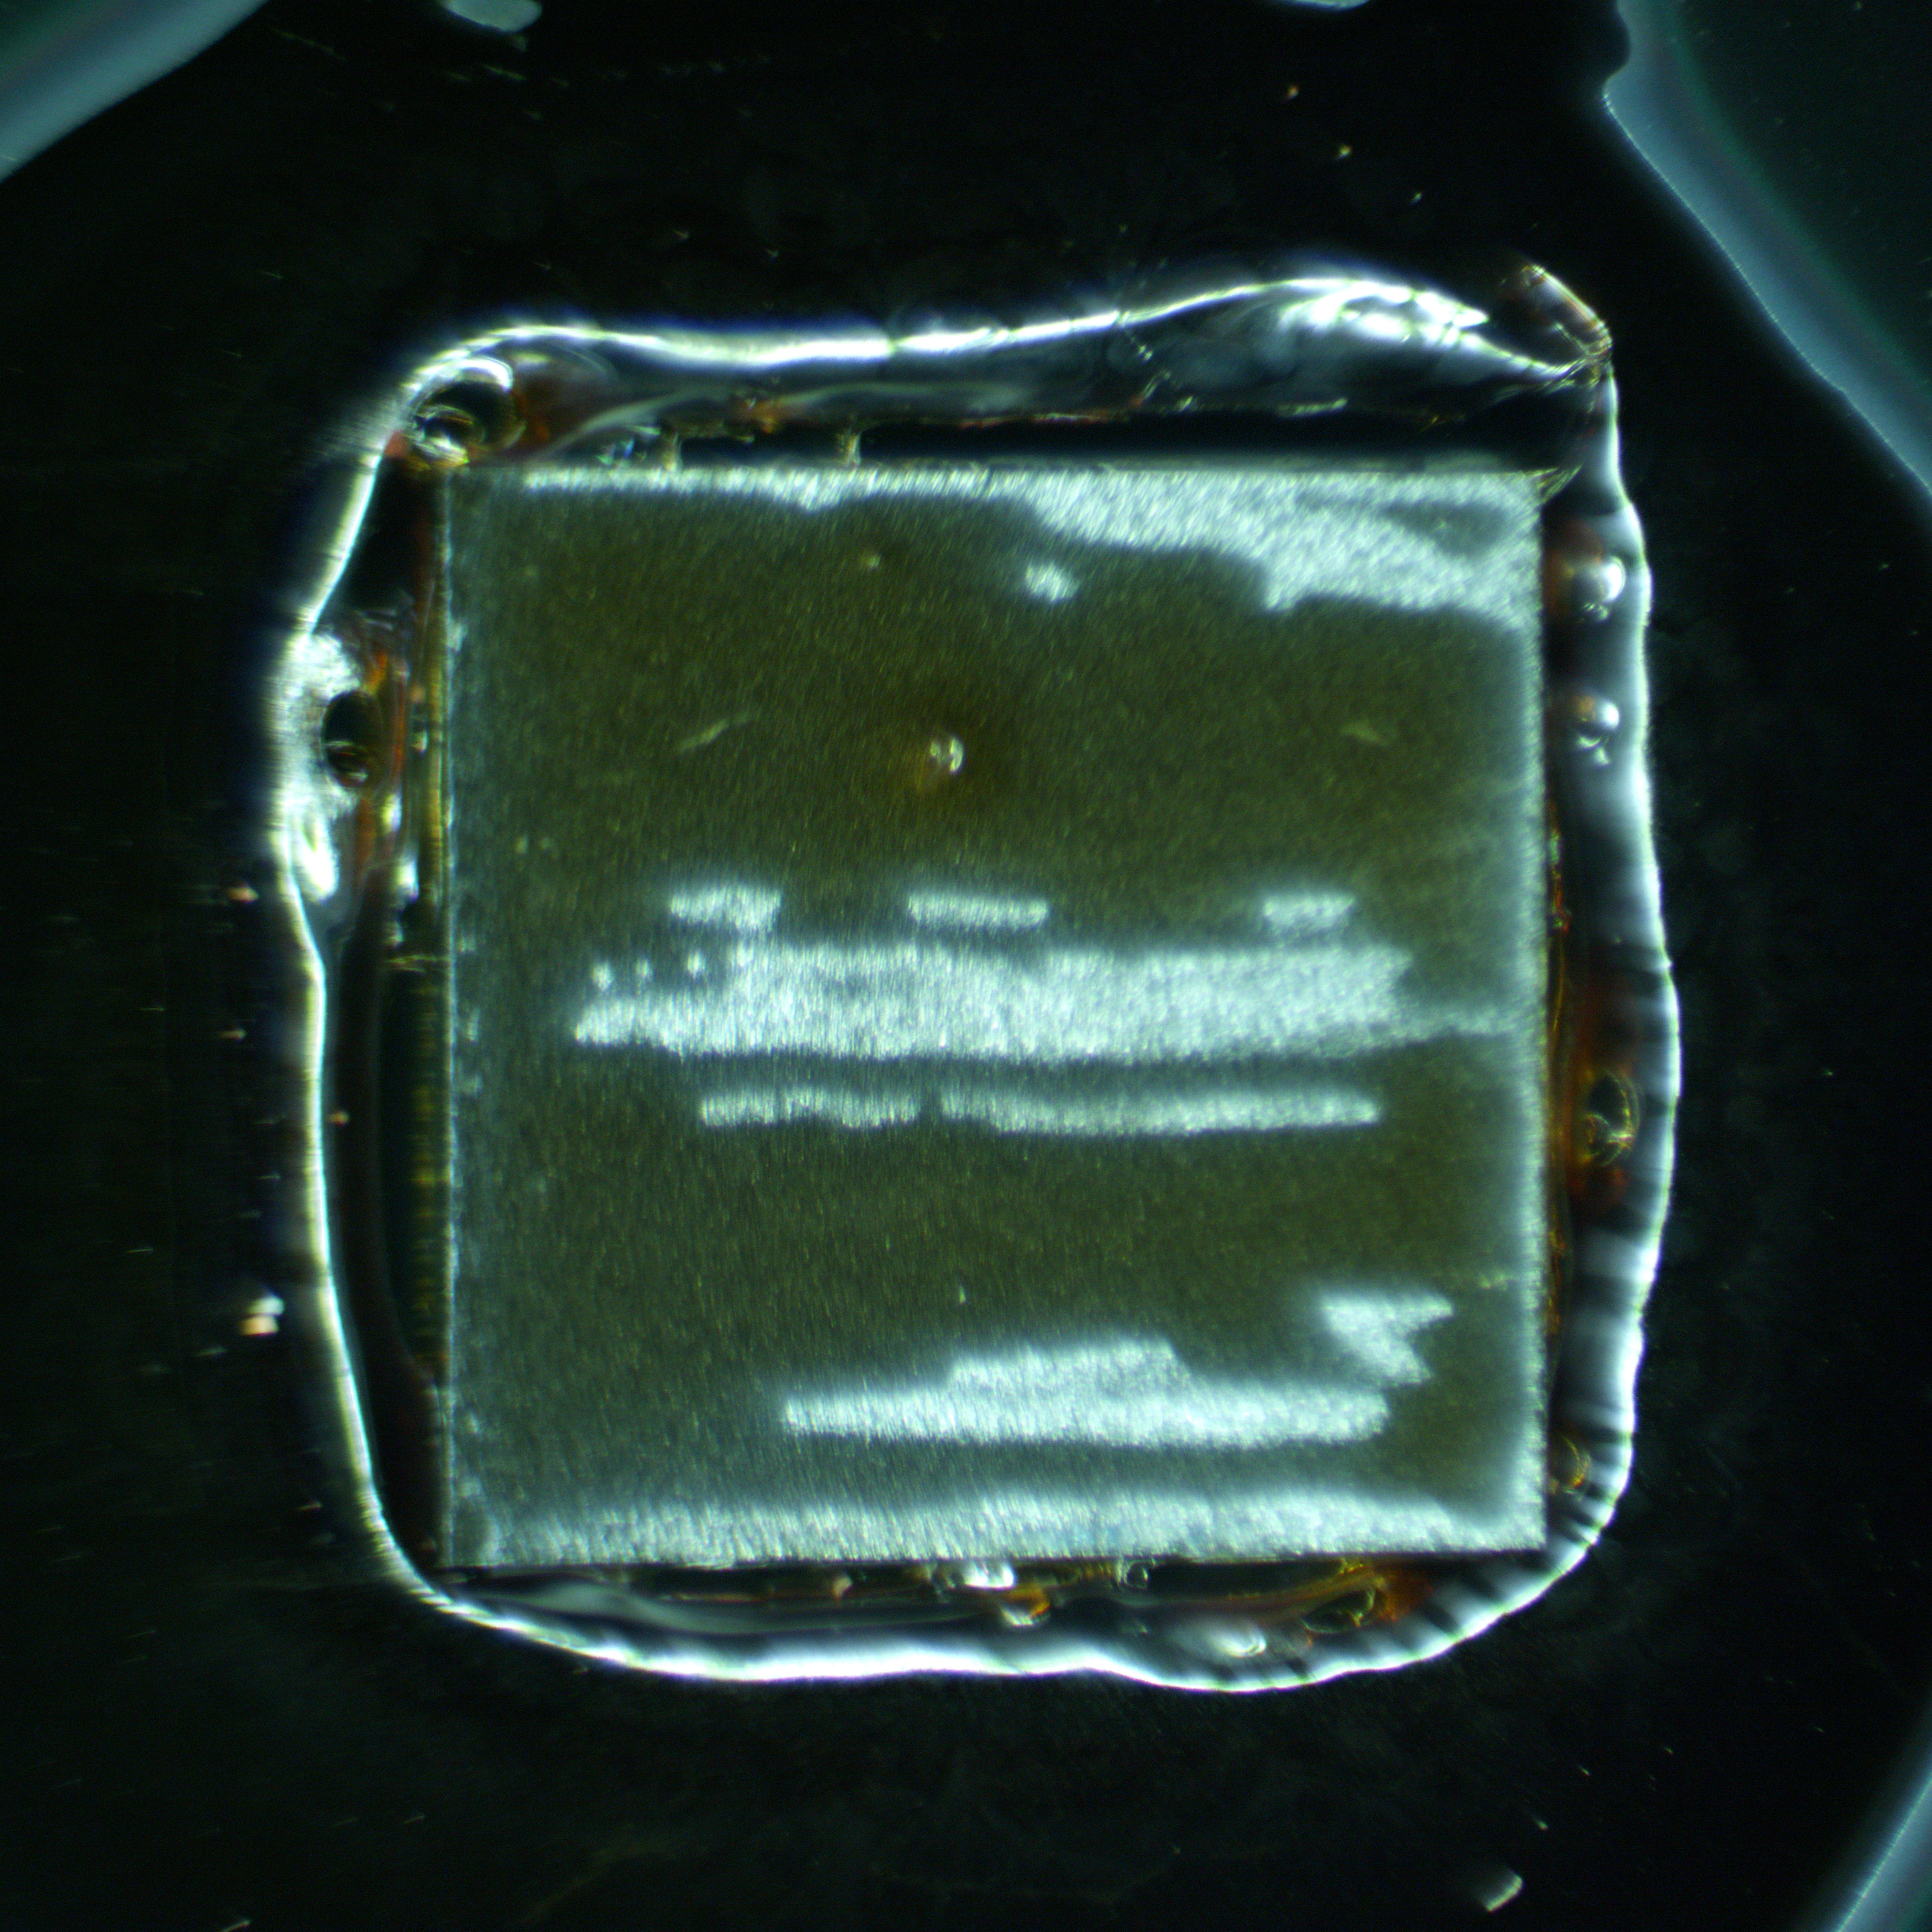
\includegraphics[width=\linewidth]{pics/spincoat/no7/7101.jpg}
        \caption{Heater 1}
    \end{subfigure}
    \hfill
    \begin{subfigure}[t]{0.3\textwidth}
        \centering
        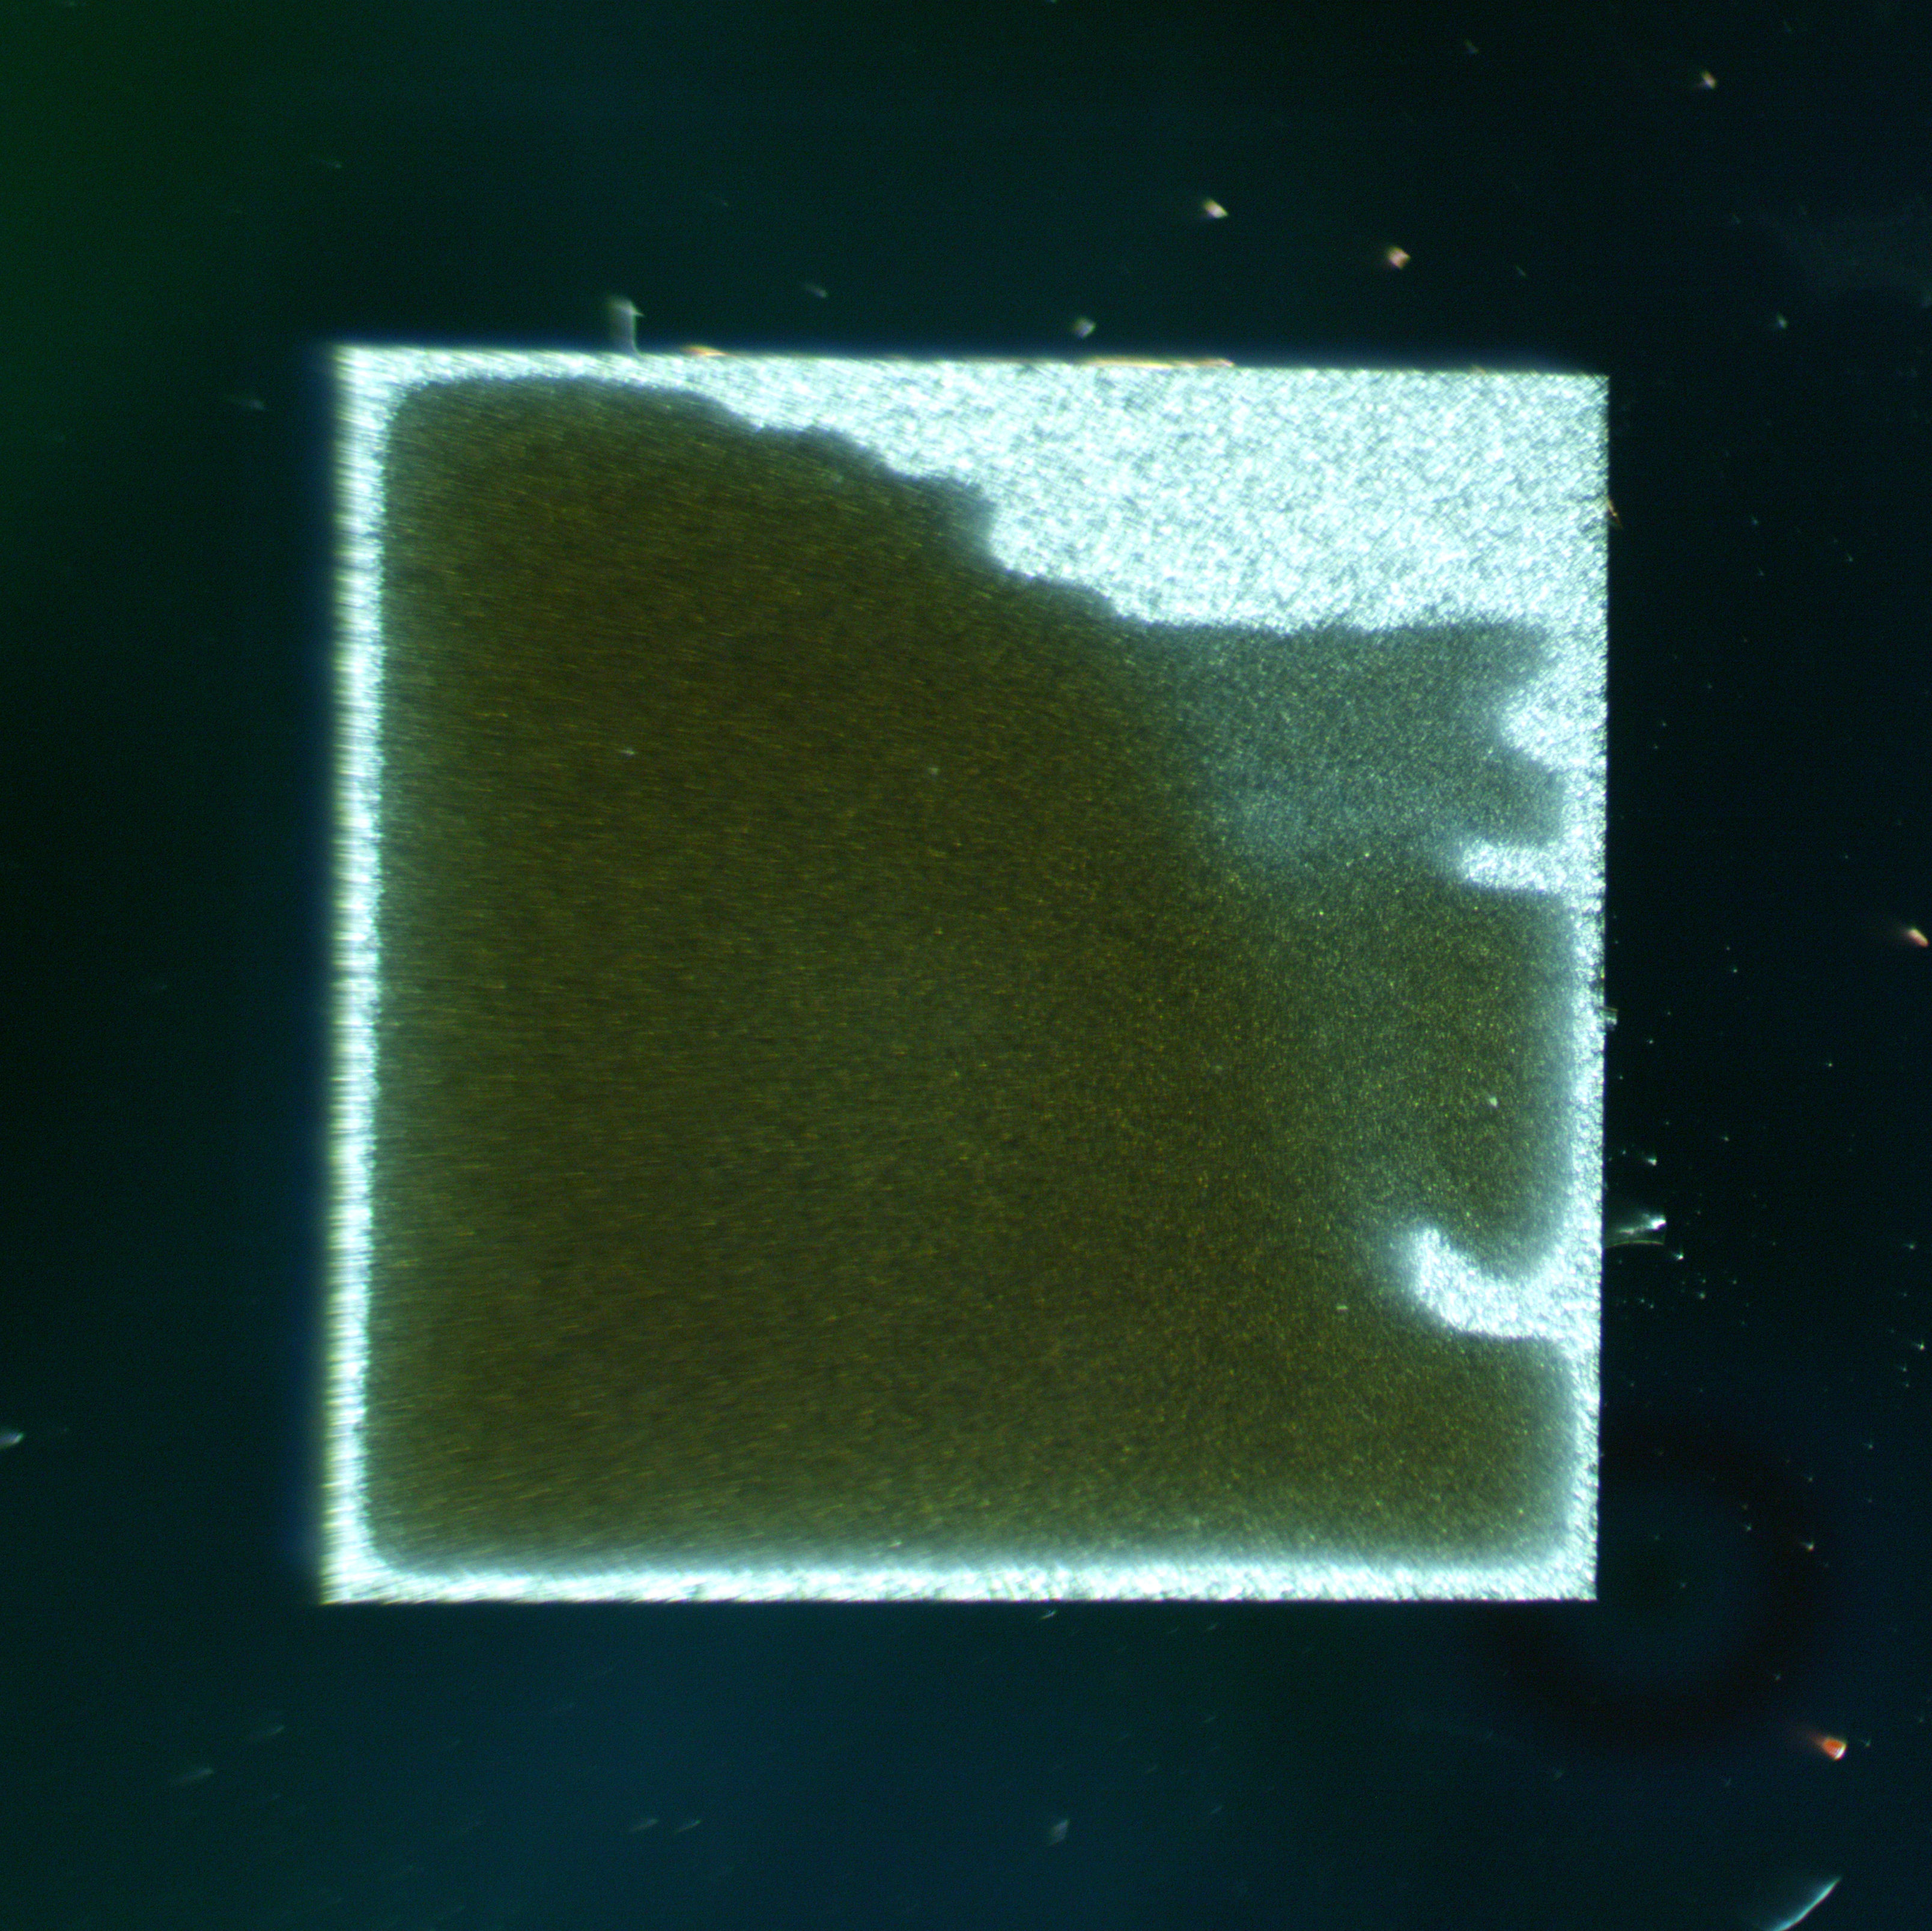
\includegraphics[width=\linewidth]{pics/spincoat/no7/7110.jpg}
        \caption{\textcolor{blue!60!black}{\textbf{Heater 2}}}
    \end{subfigure}
    \hfill
    \begin{subfigure}[t]{0.3\textwidth}
        \centering
        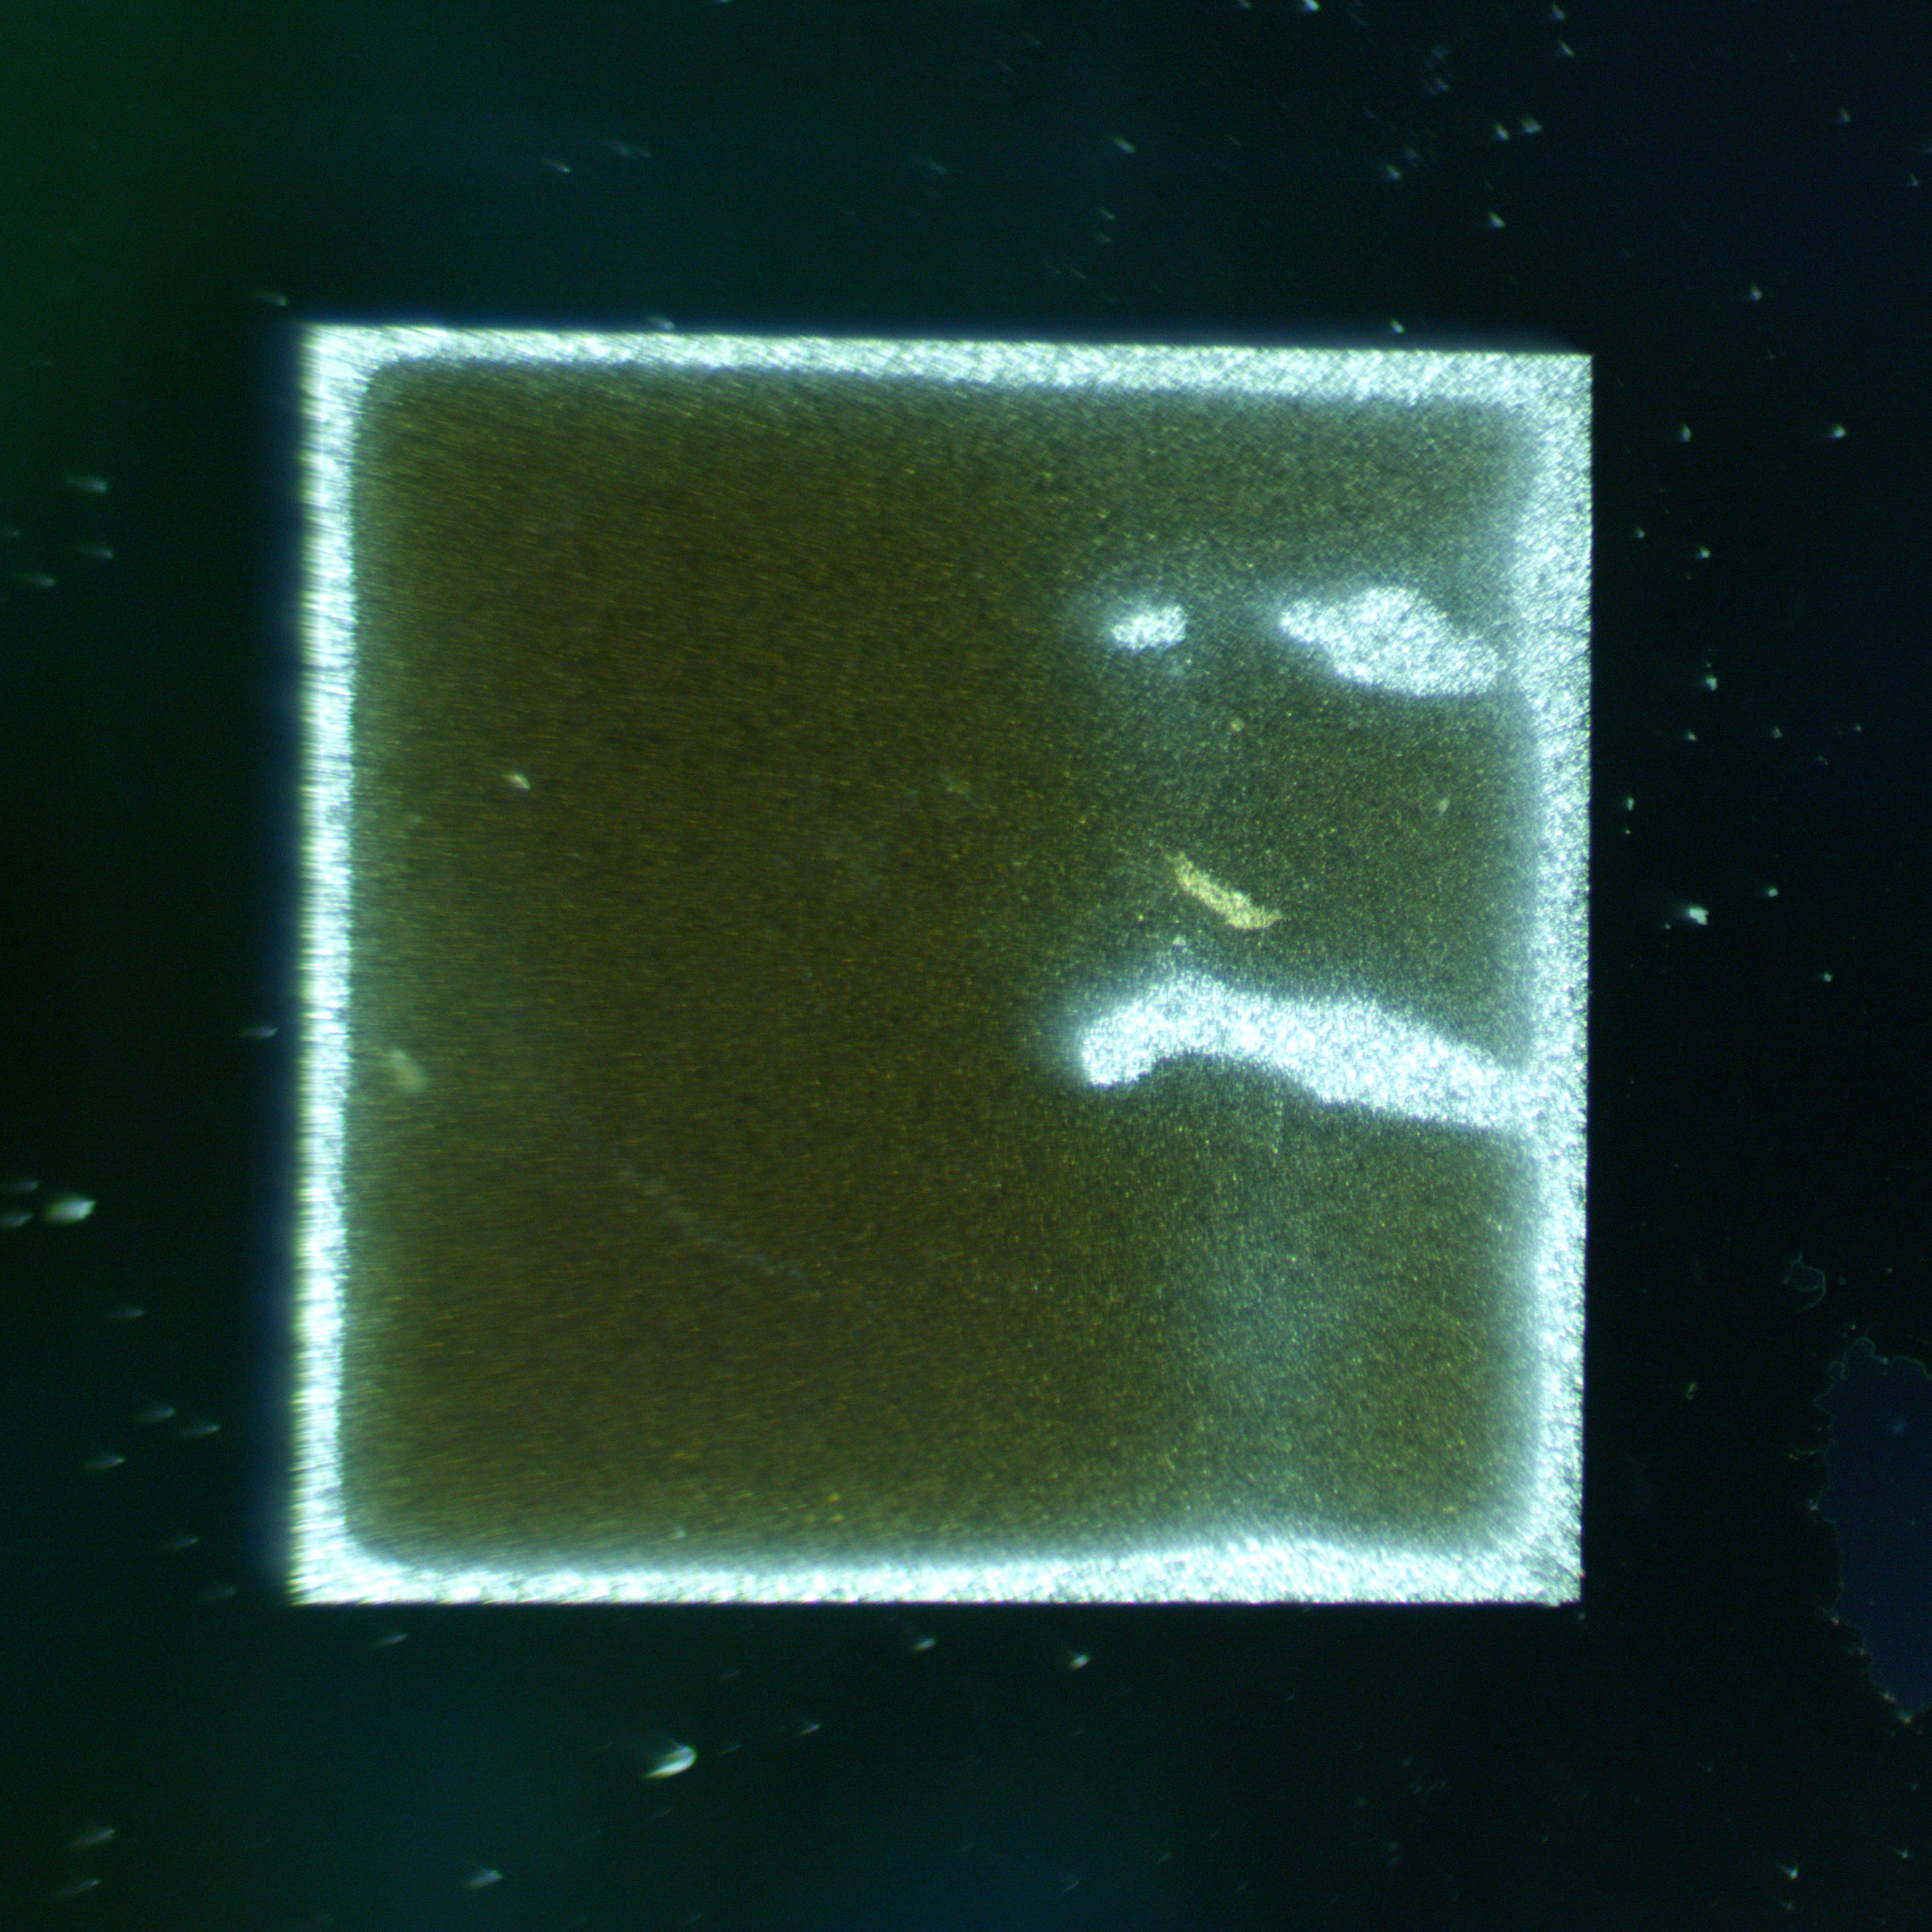
\includegraphics[width=\linewidth]{pics/spincoat/no7/7111.jpg}
        \caption{\textcolor{blue!60!black}{\textbf{Heater 3*}}}
    \end{subfigure}

    \vspace{0.8cm}

    % ---------- Row 2 ----------
    \begin{subfigure}[t]{0.3\textwidth}
        \centering
        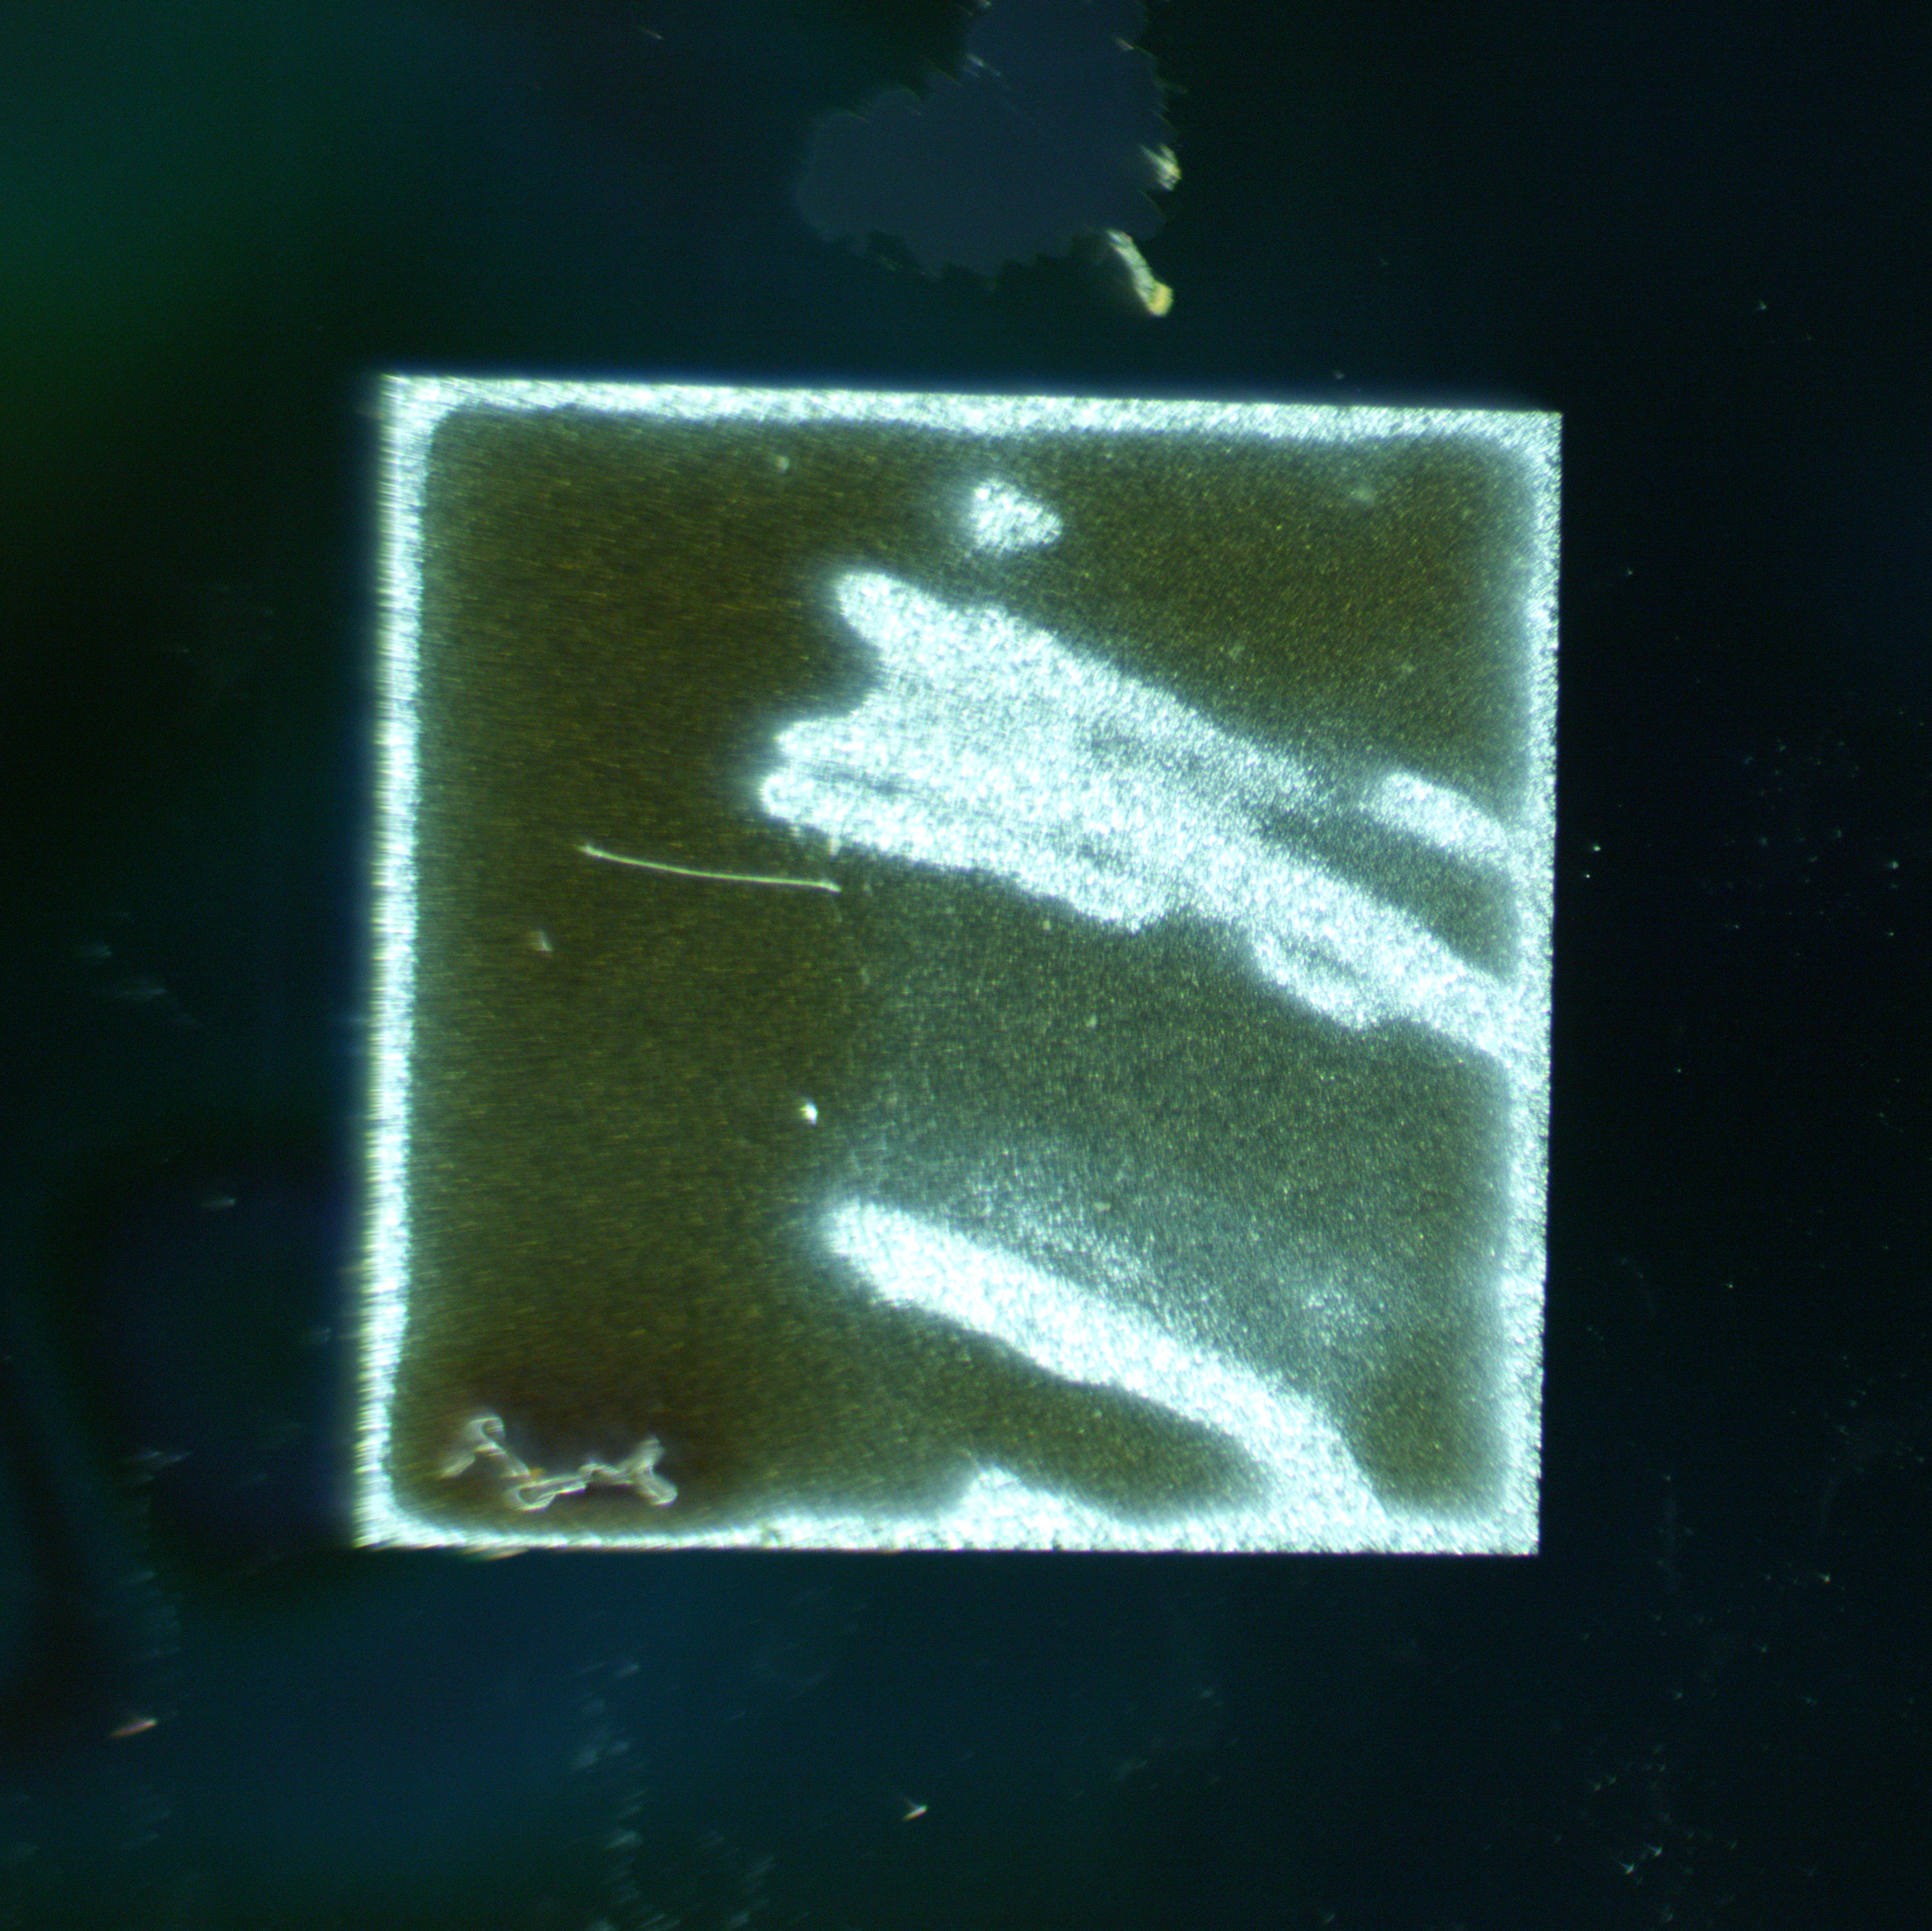
\includegraphics[width=\linewidth]{pics/spincoat/no7/7112.jpg}
        \caption{\textcolor{blue!60!black}{\textbf{Heater 4*}}}
    \end{subfigure}
    \hfill
    \begin{subfigure}[t]{0.3\textwidth}
        \centering
        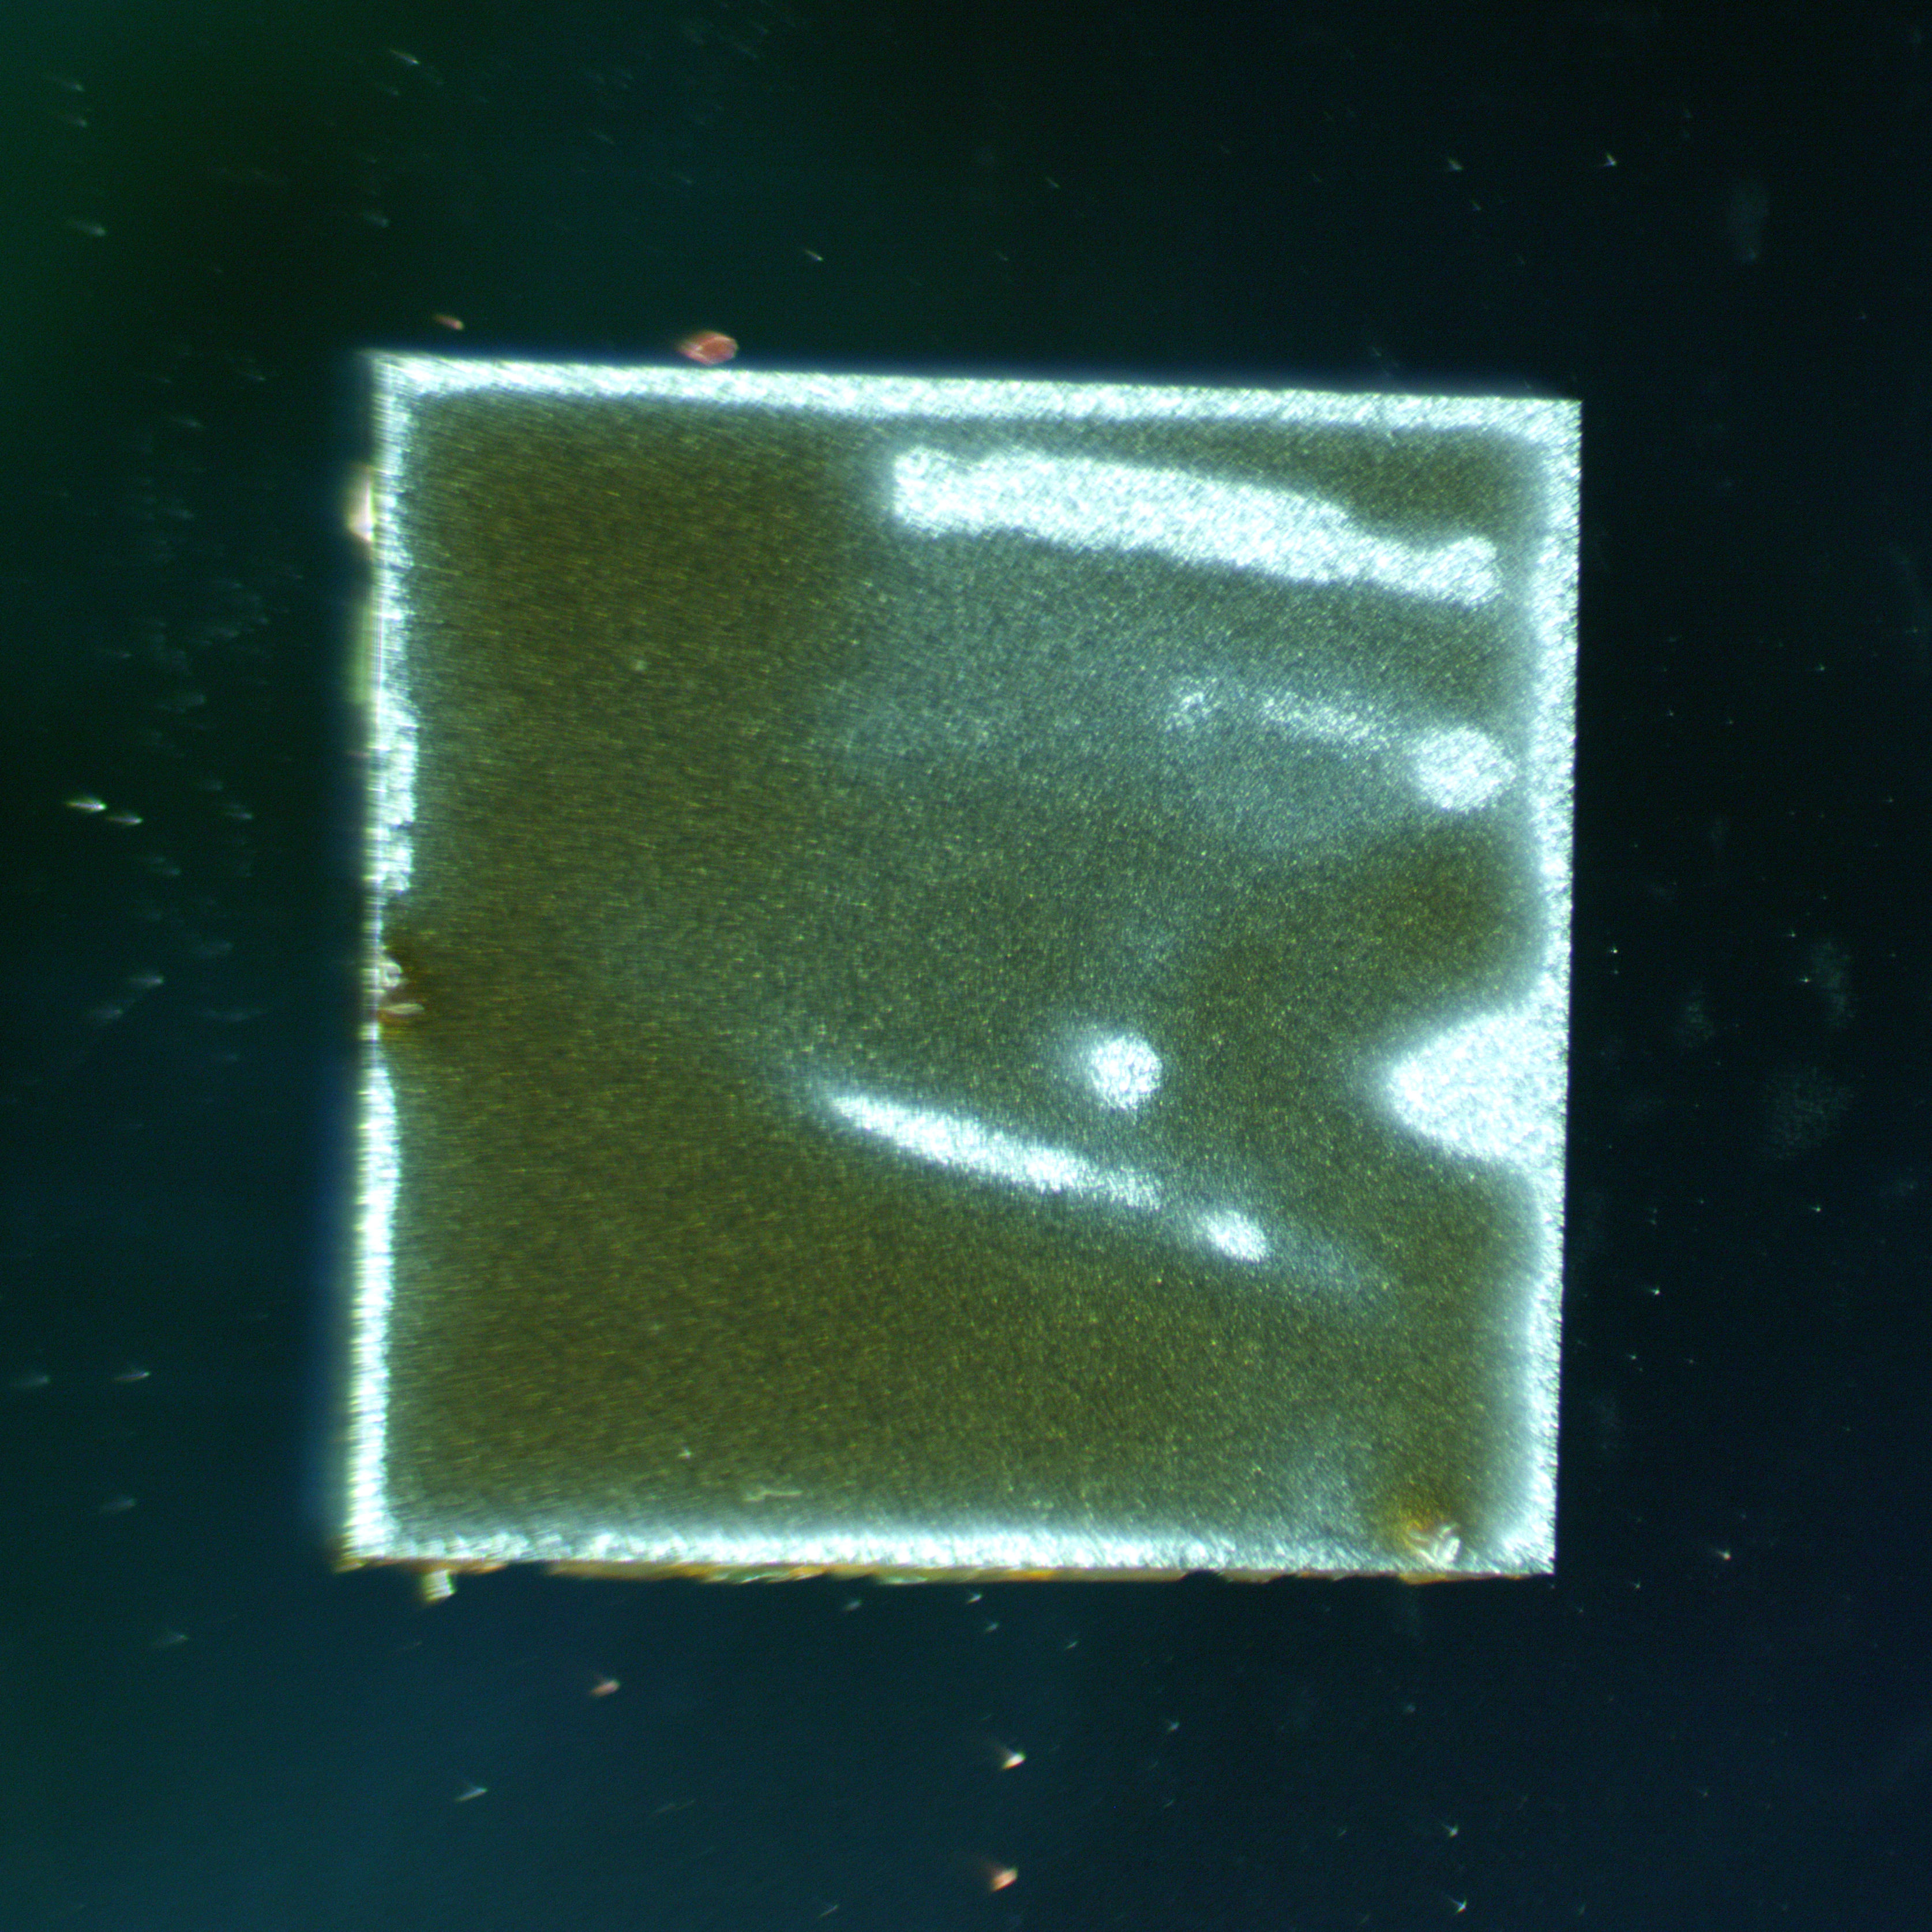
\includegraphics[width=\linewidth]{pics/spincoat/no7/7113.jpg}
        \caption{\textcolor{blue!60!black}{\textbf{Heater 5}}}
    \end{subfigure}
    \hfill
    \begin{subfigure}[t]{0.3\textwidth}
        \centering
        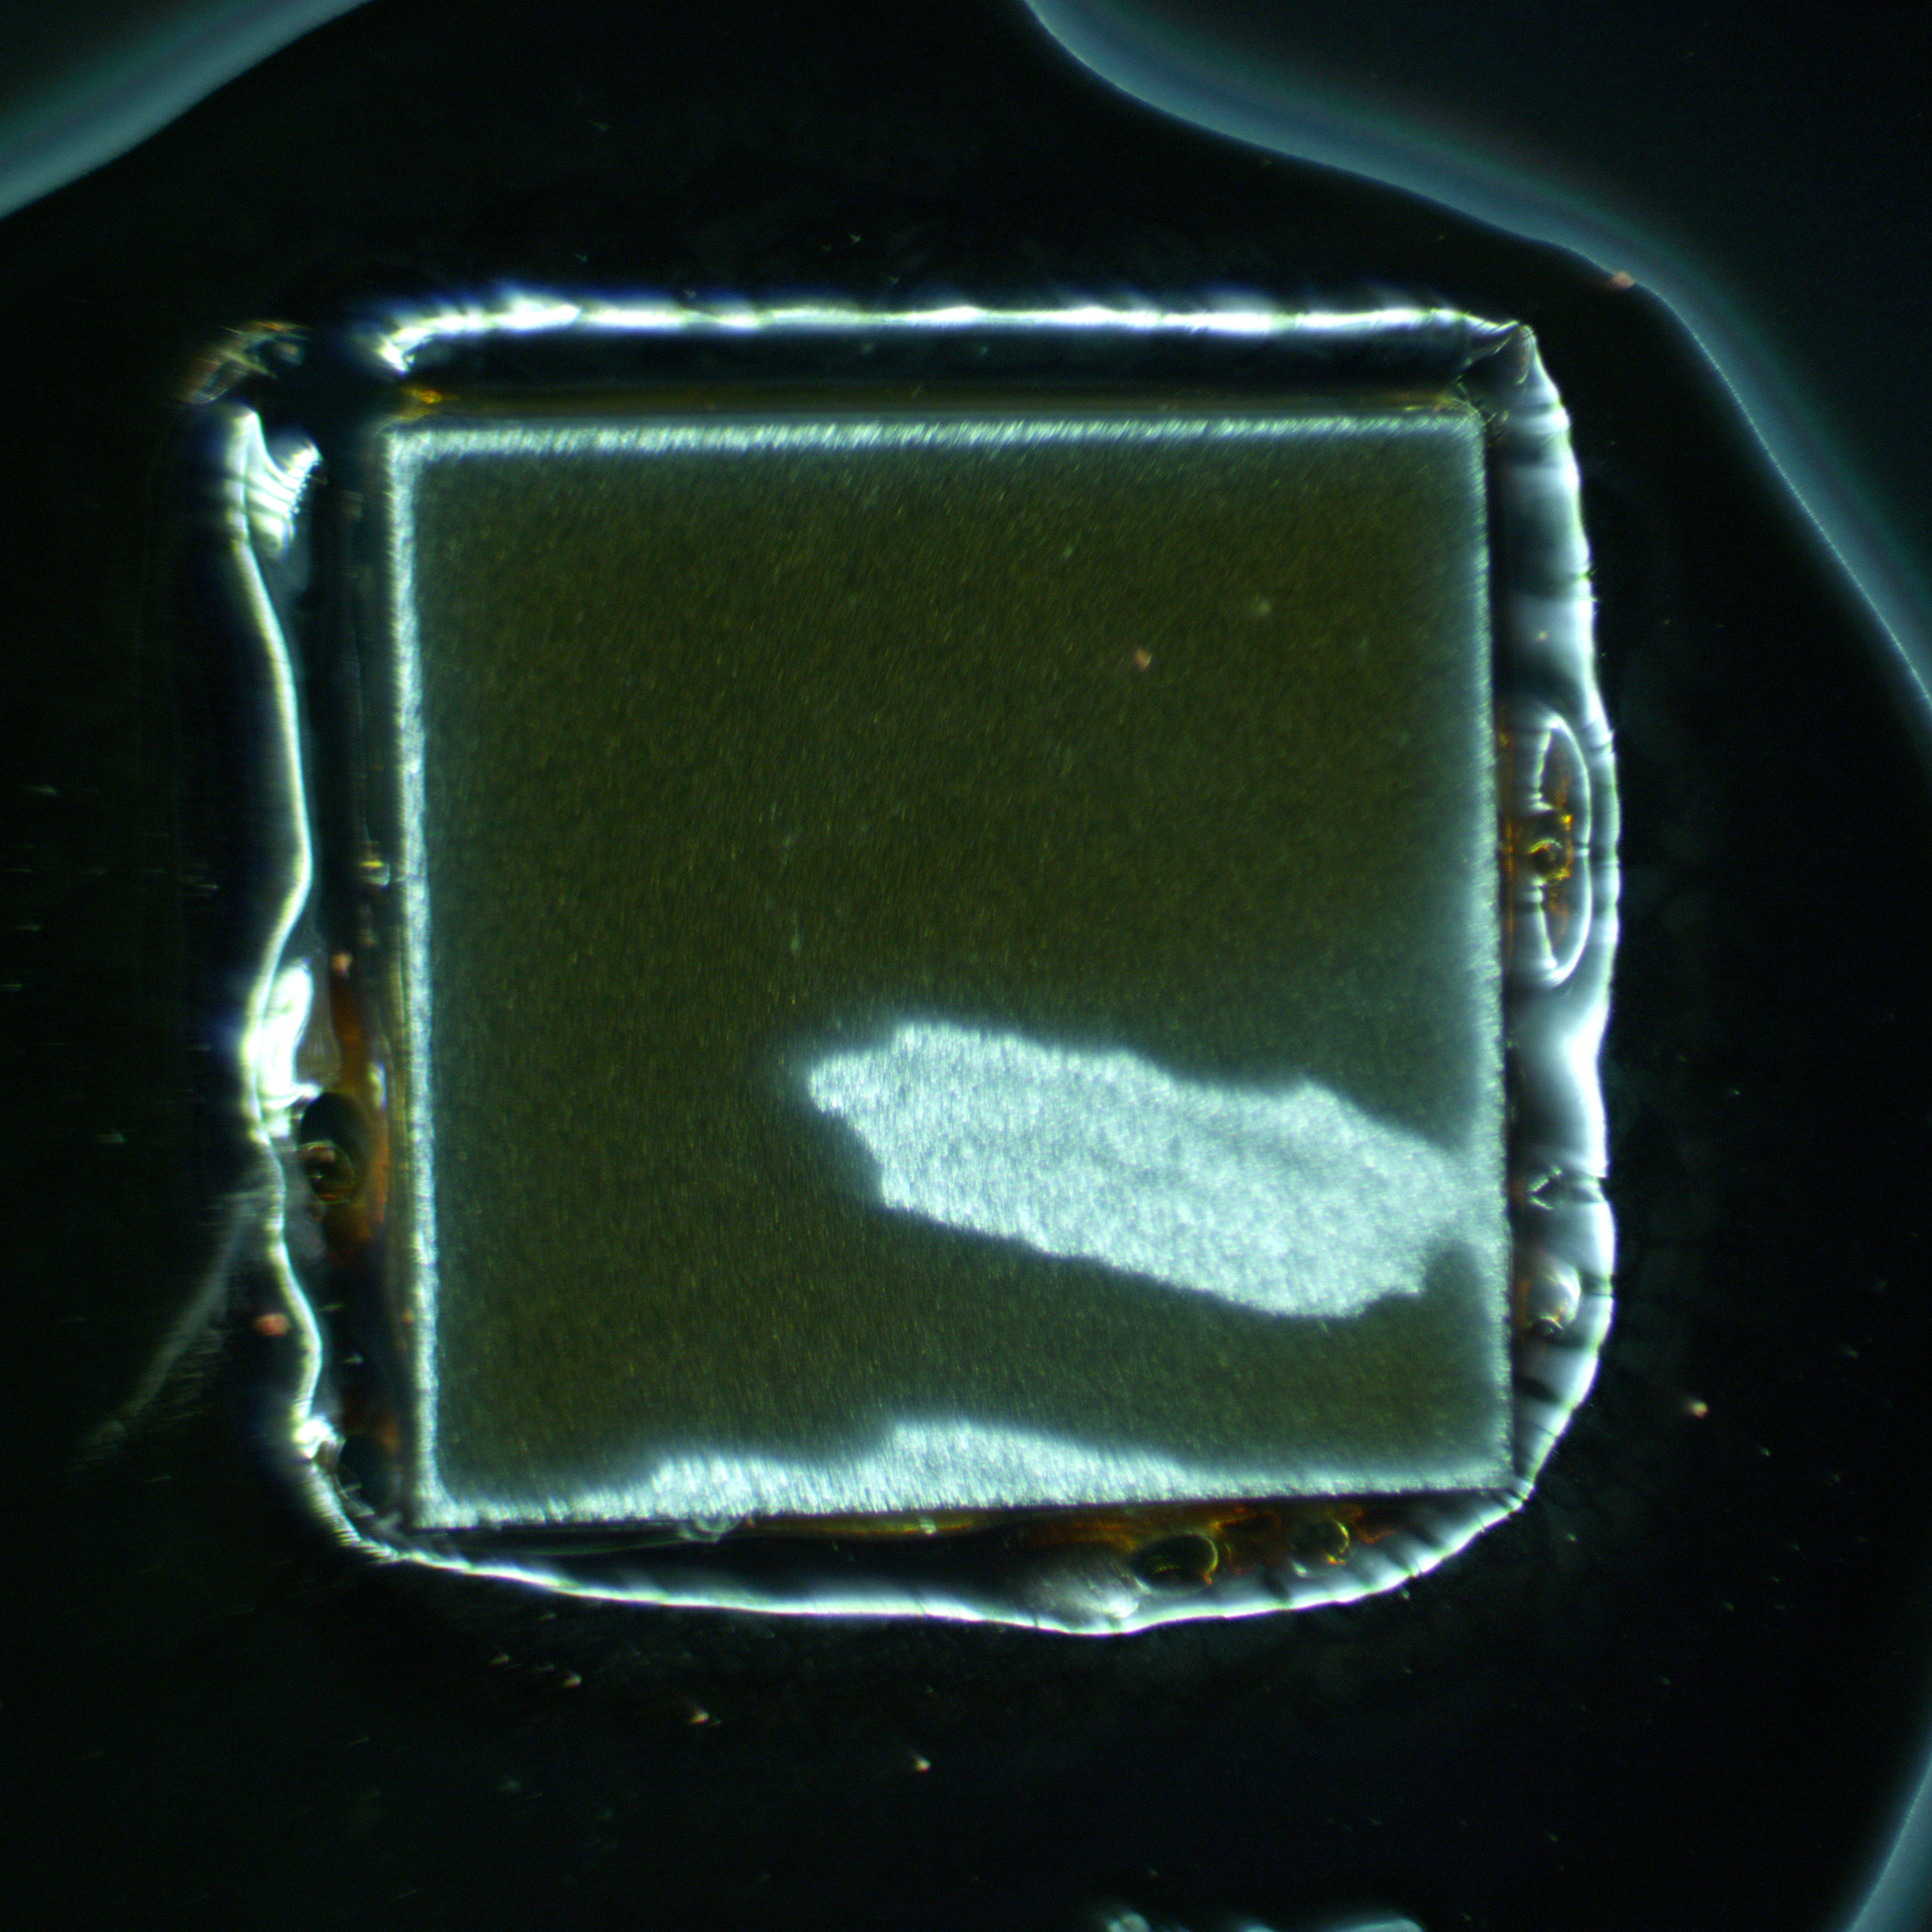
\includegraphics[width=\linewidth]{pics/spincoat/no7/7106.jpg}
        \caption{Heater 6}
    \end{subfigure}

    \vspace{0.8cm}

    % ---------- Row 3 ----------
    \begin{subfigure}[t]{0.3\textwidth}
        \centering
        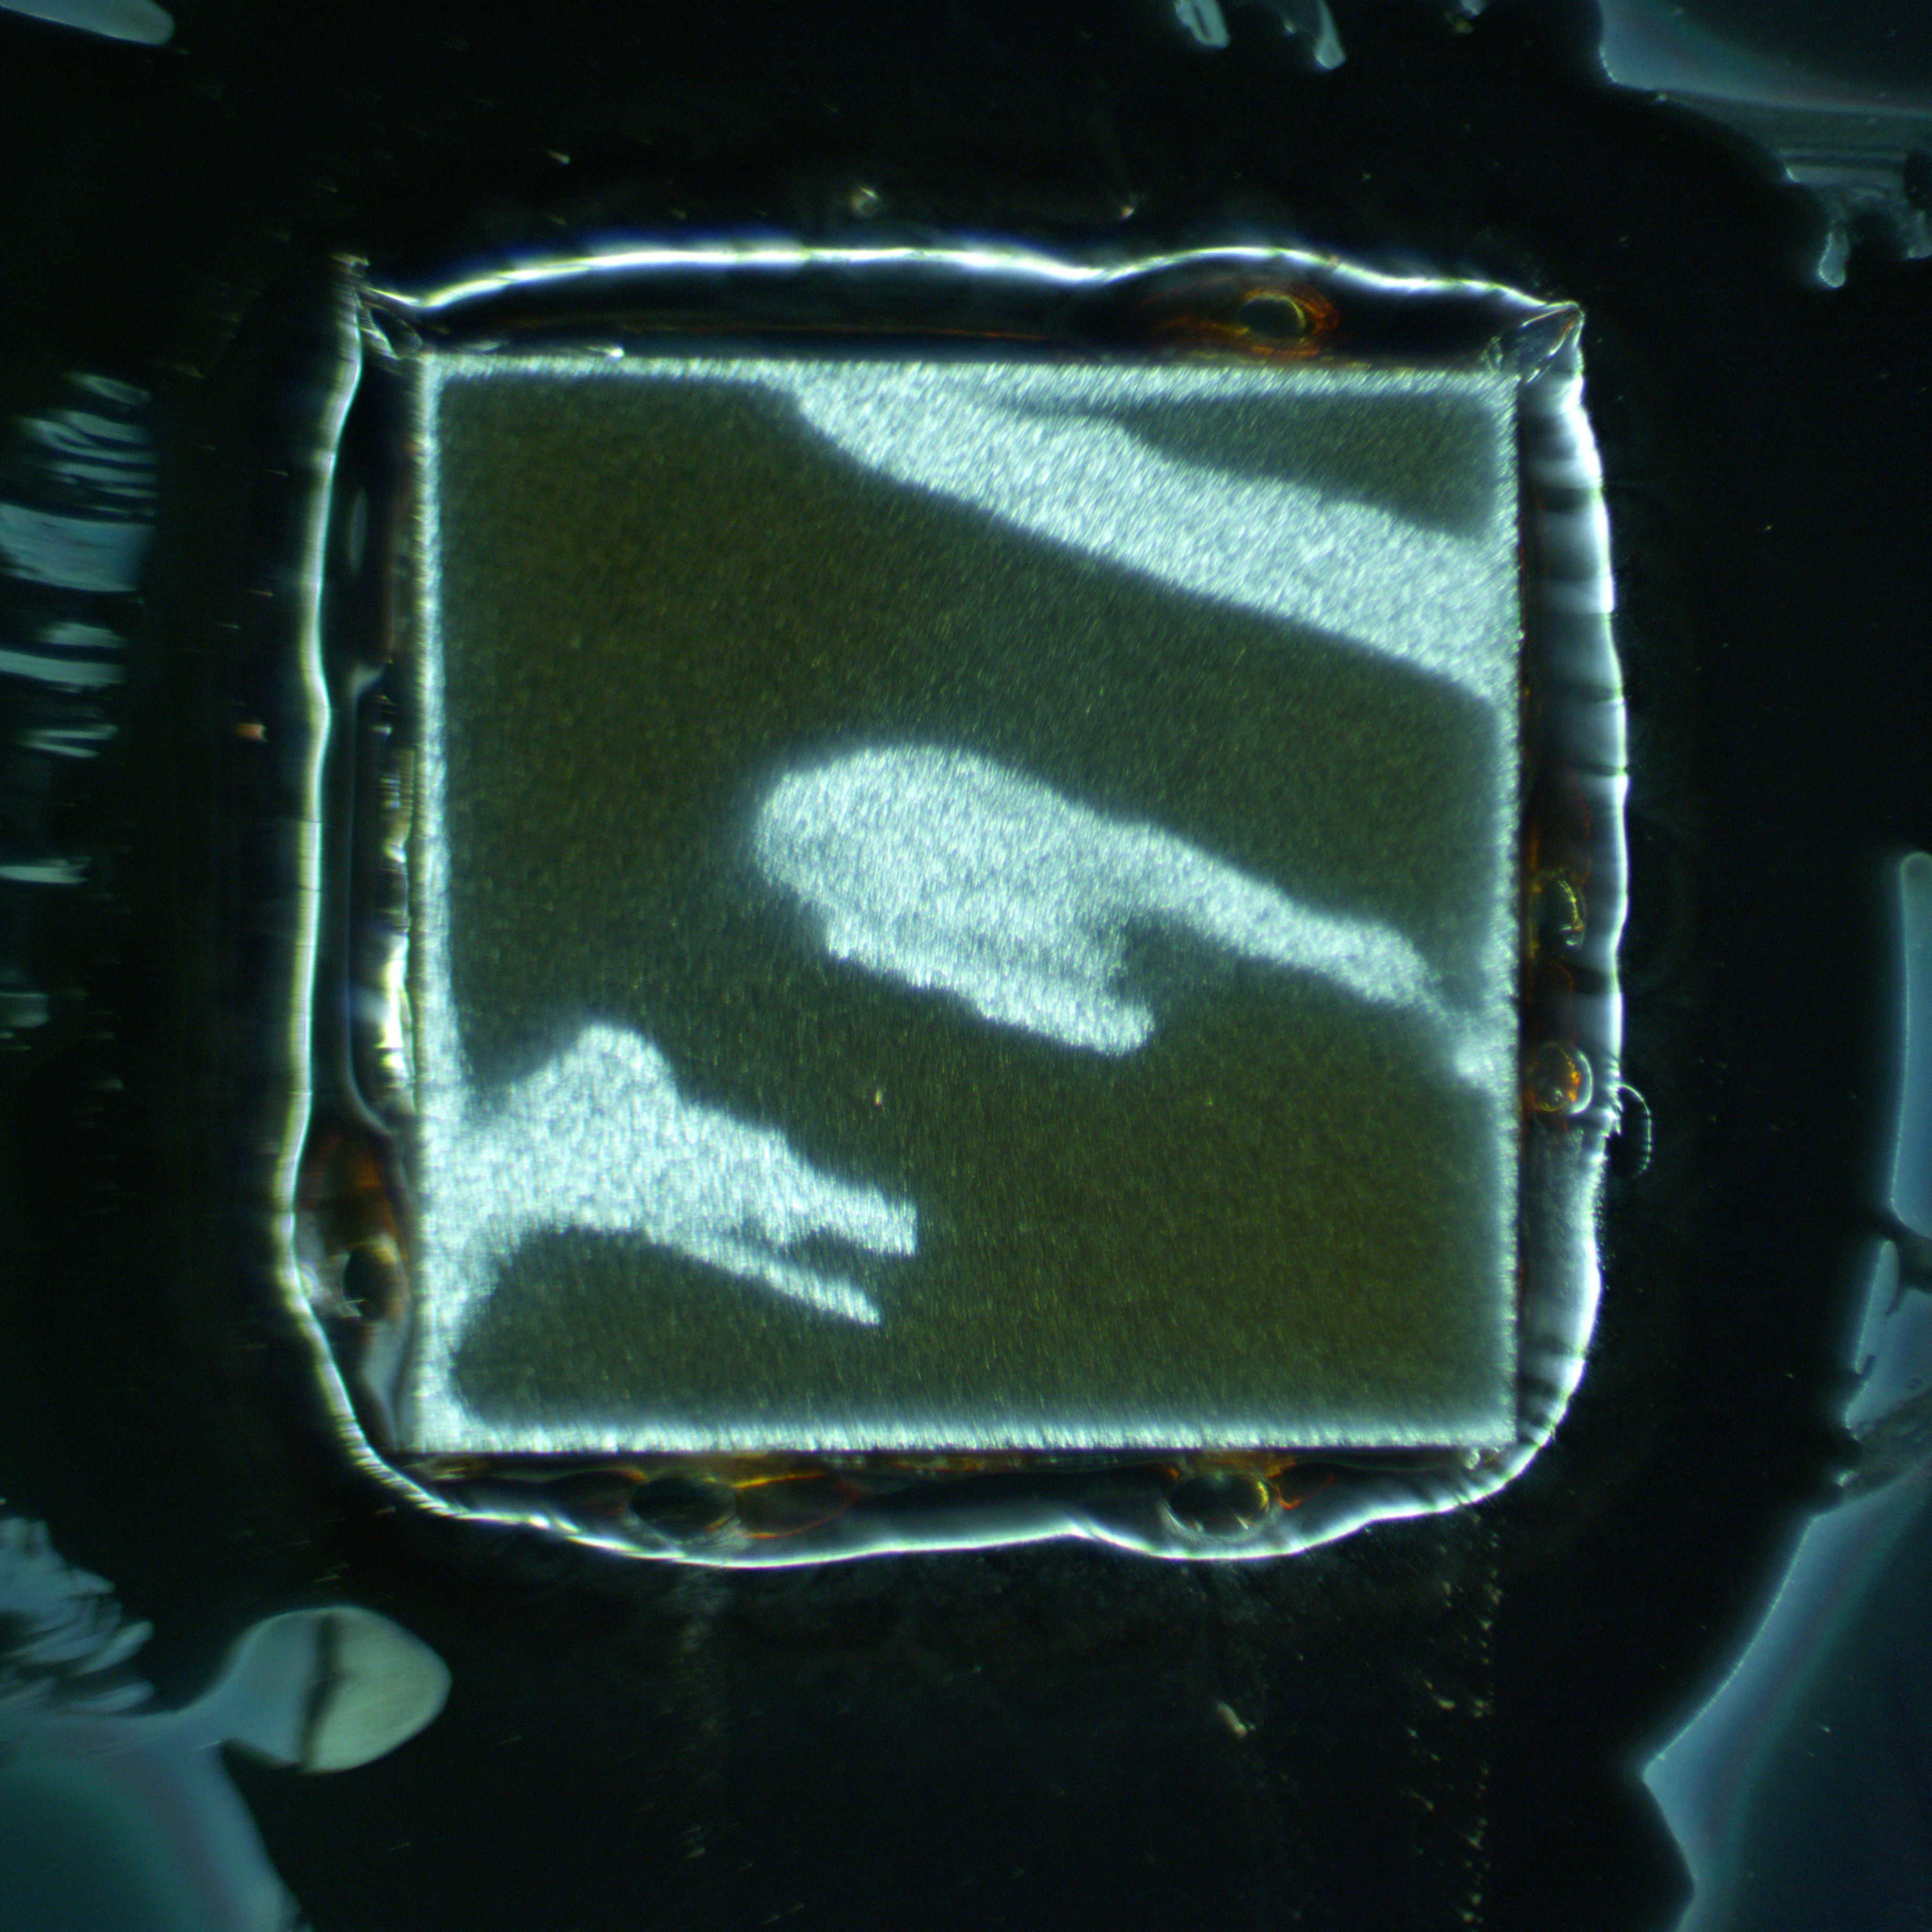
\includegraphics[width=\linewidth]{pics/spincoat/no7/7107.jpg}
        \caption{Heater 7}
    \end{subfigure}
    \hfill
    \begin{subfigure}[t]{0.3\textwidth}
        \centering
        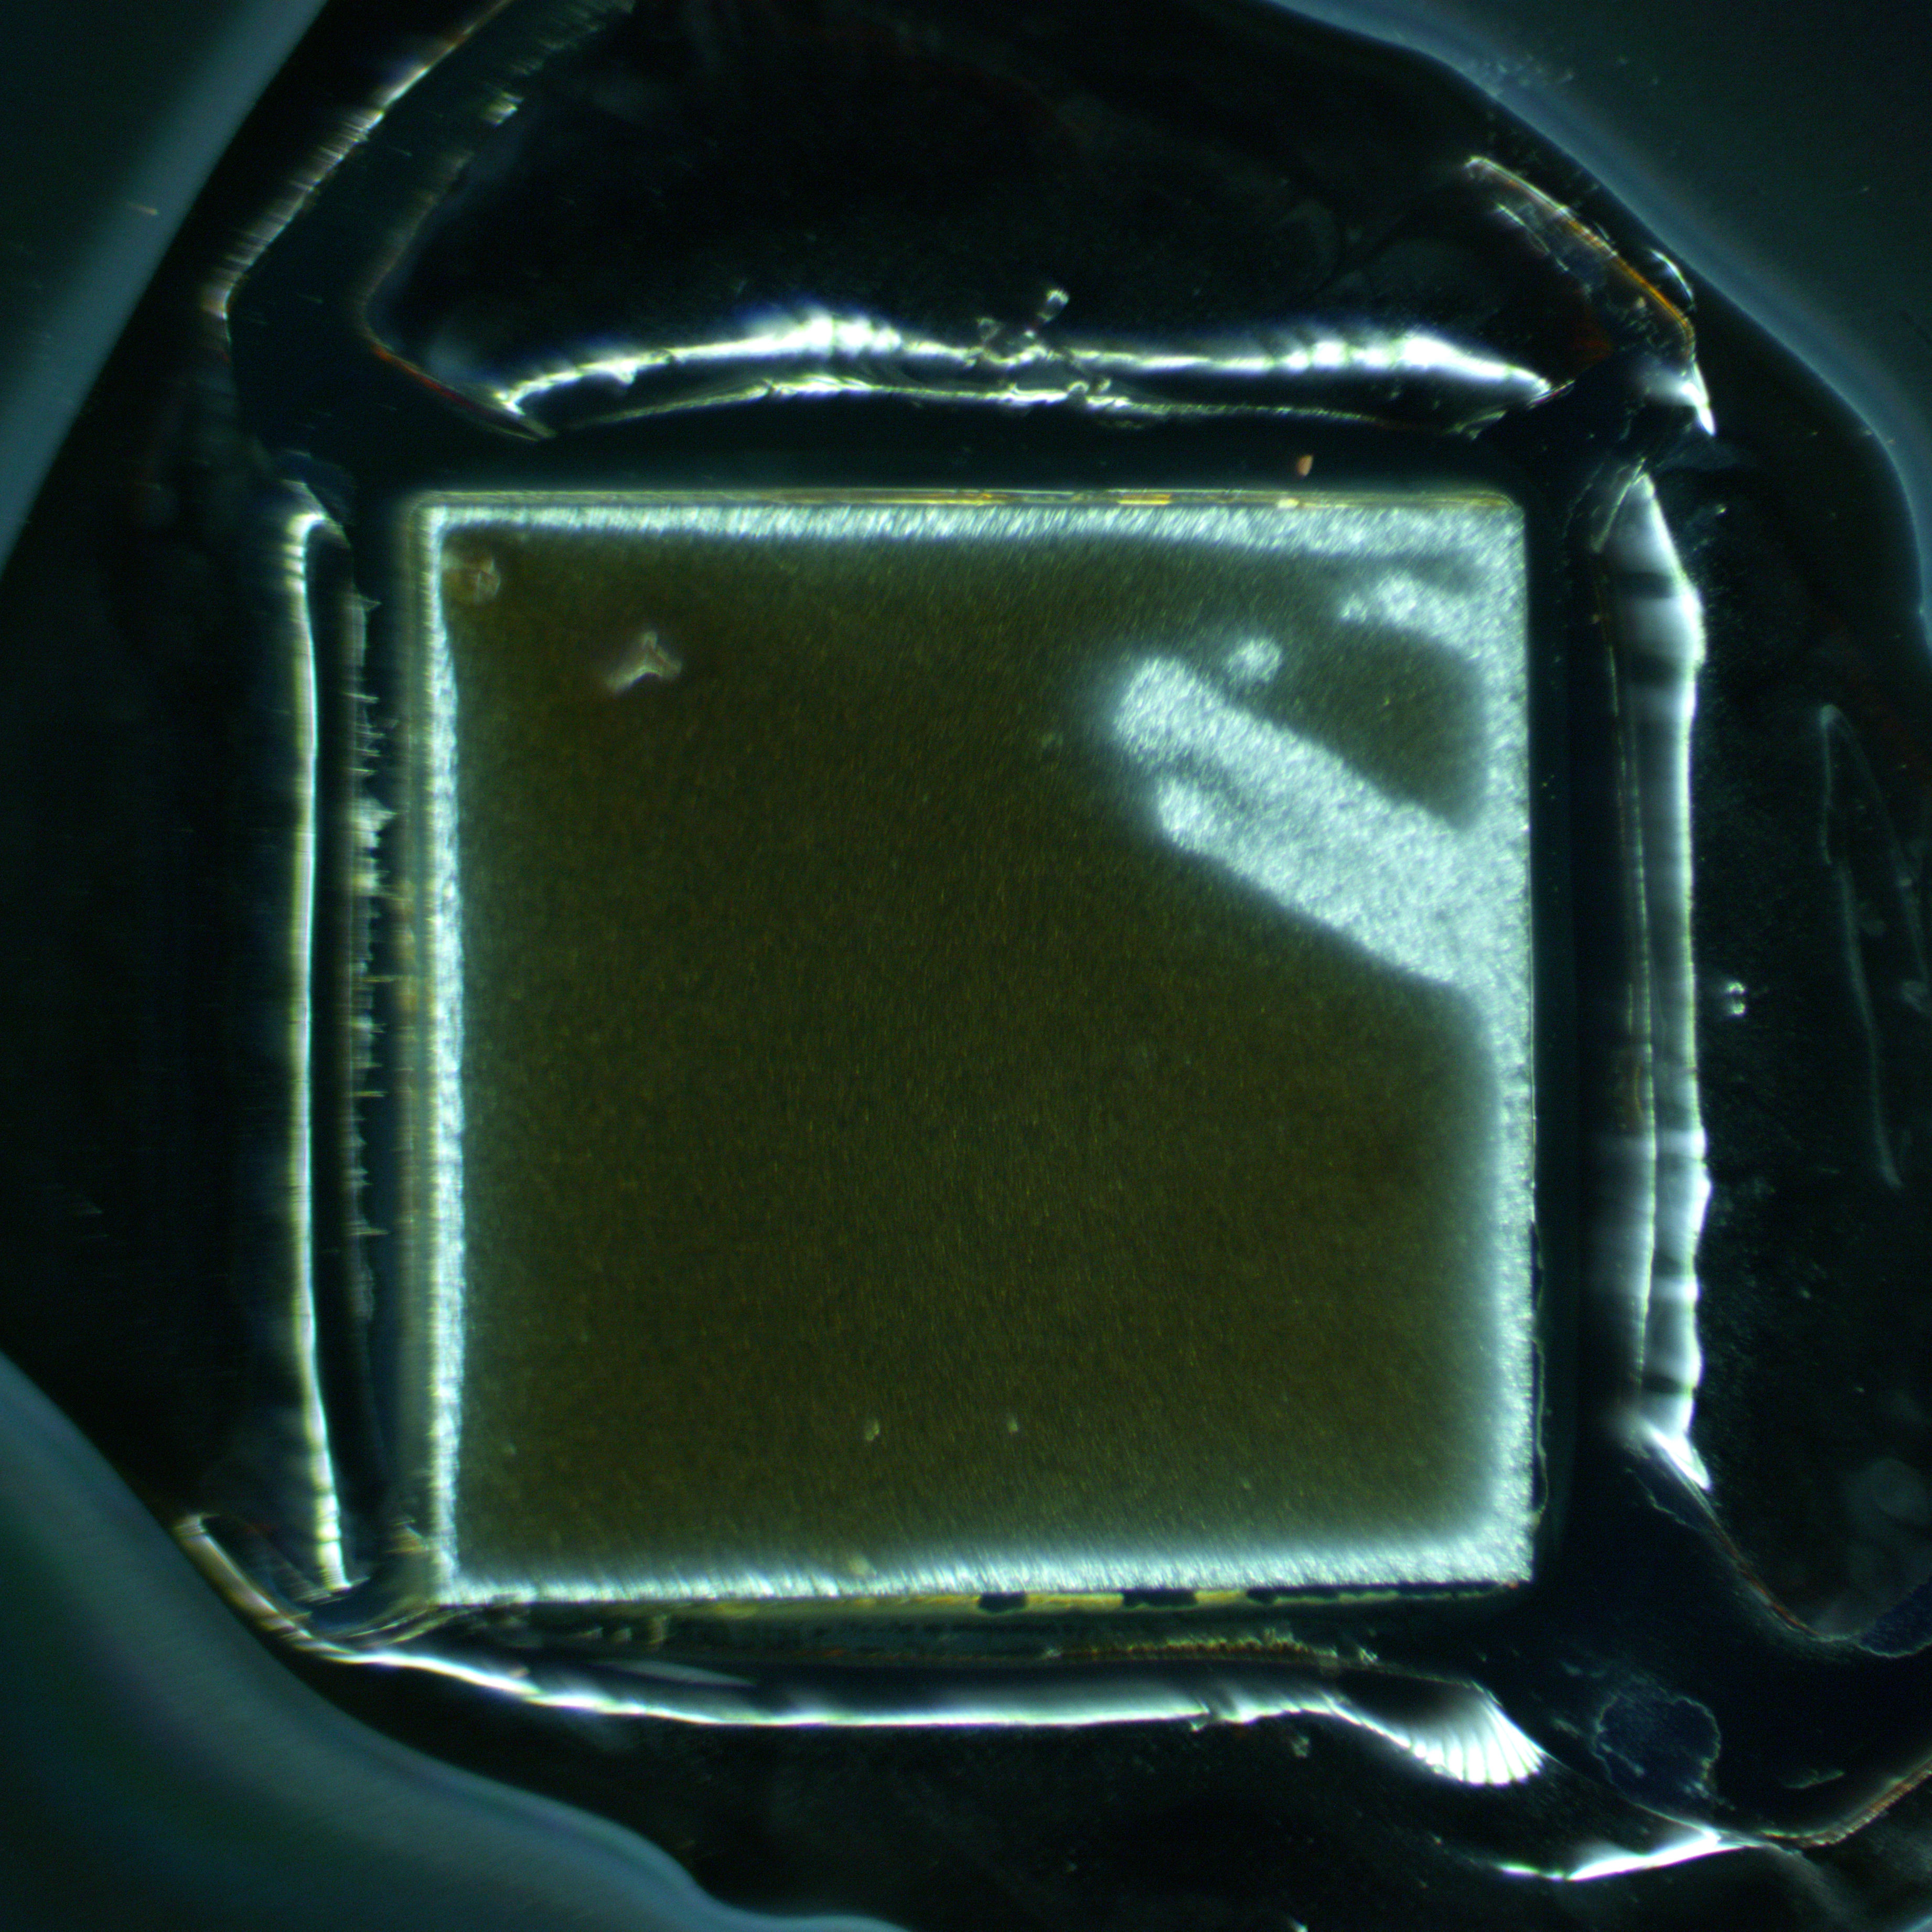
\includegraphics[width=\linewidth]{pics/spincoat/no7/7108.jpg}
        \caption{Heater 8}
    \end{subfigure}
    \hfill
    \begin{subfigure}[t]{0.3\textwidth}
        \centering
        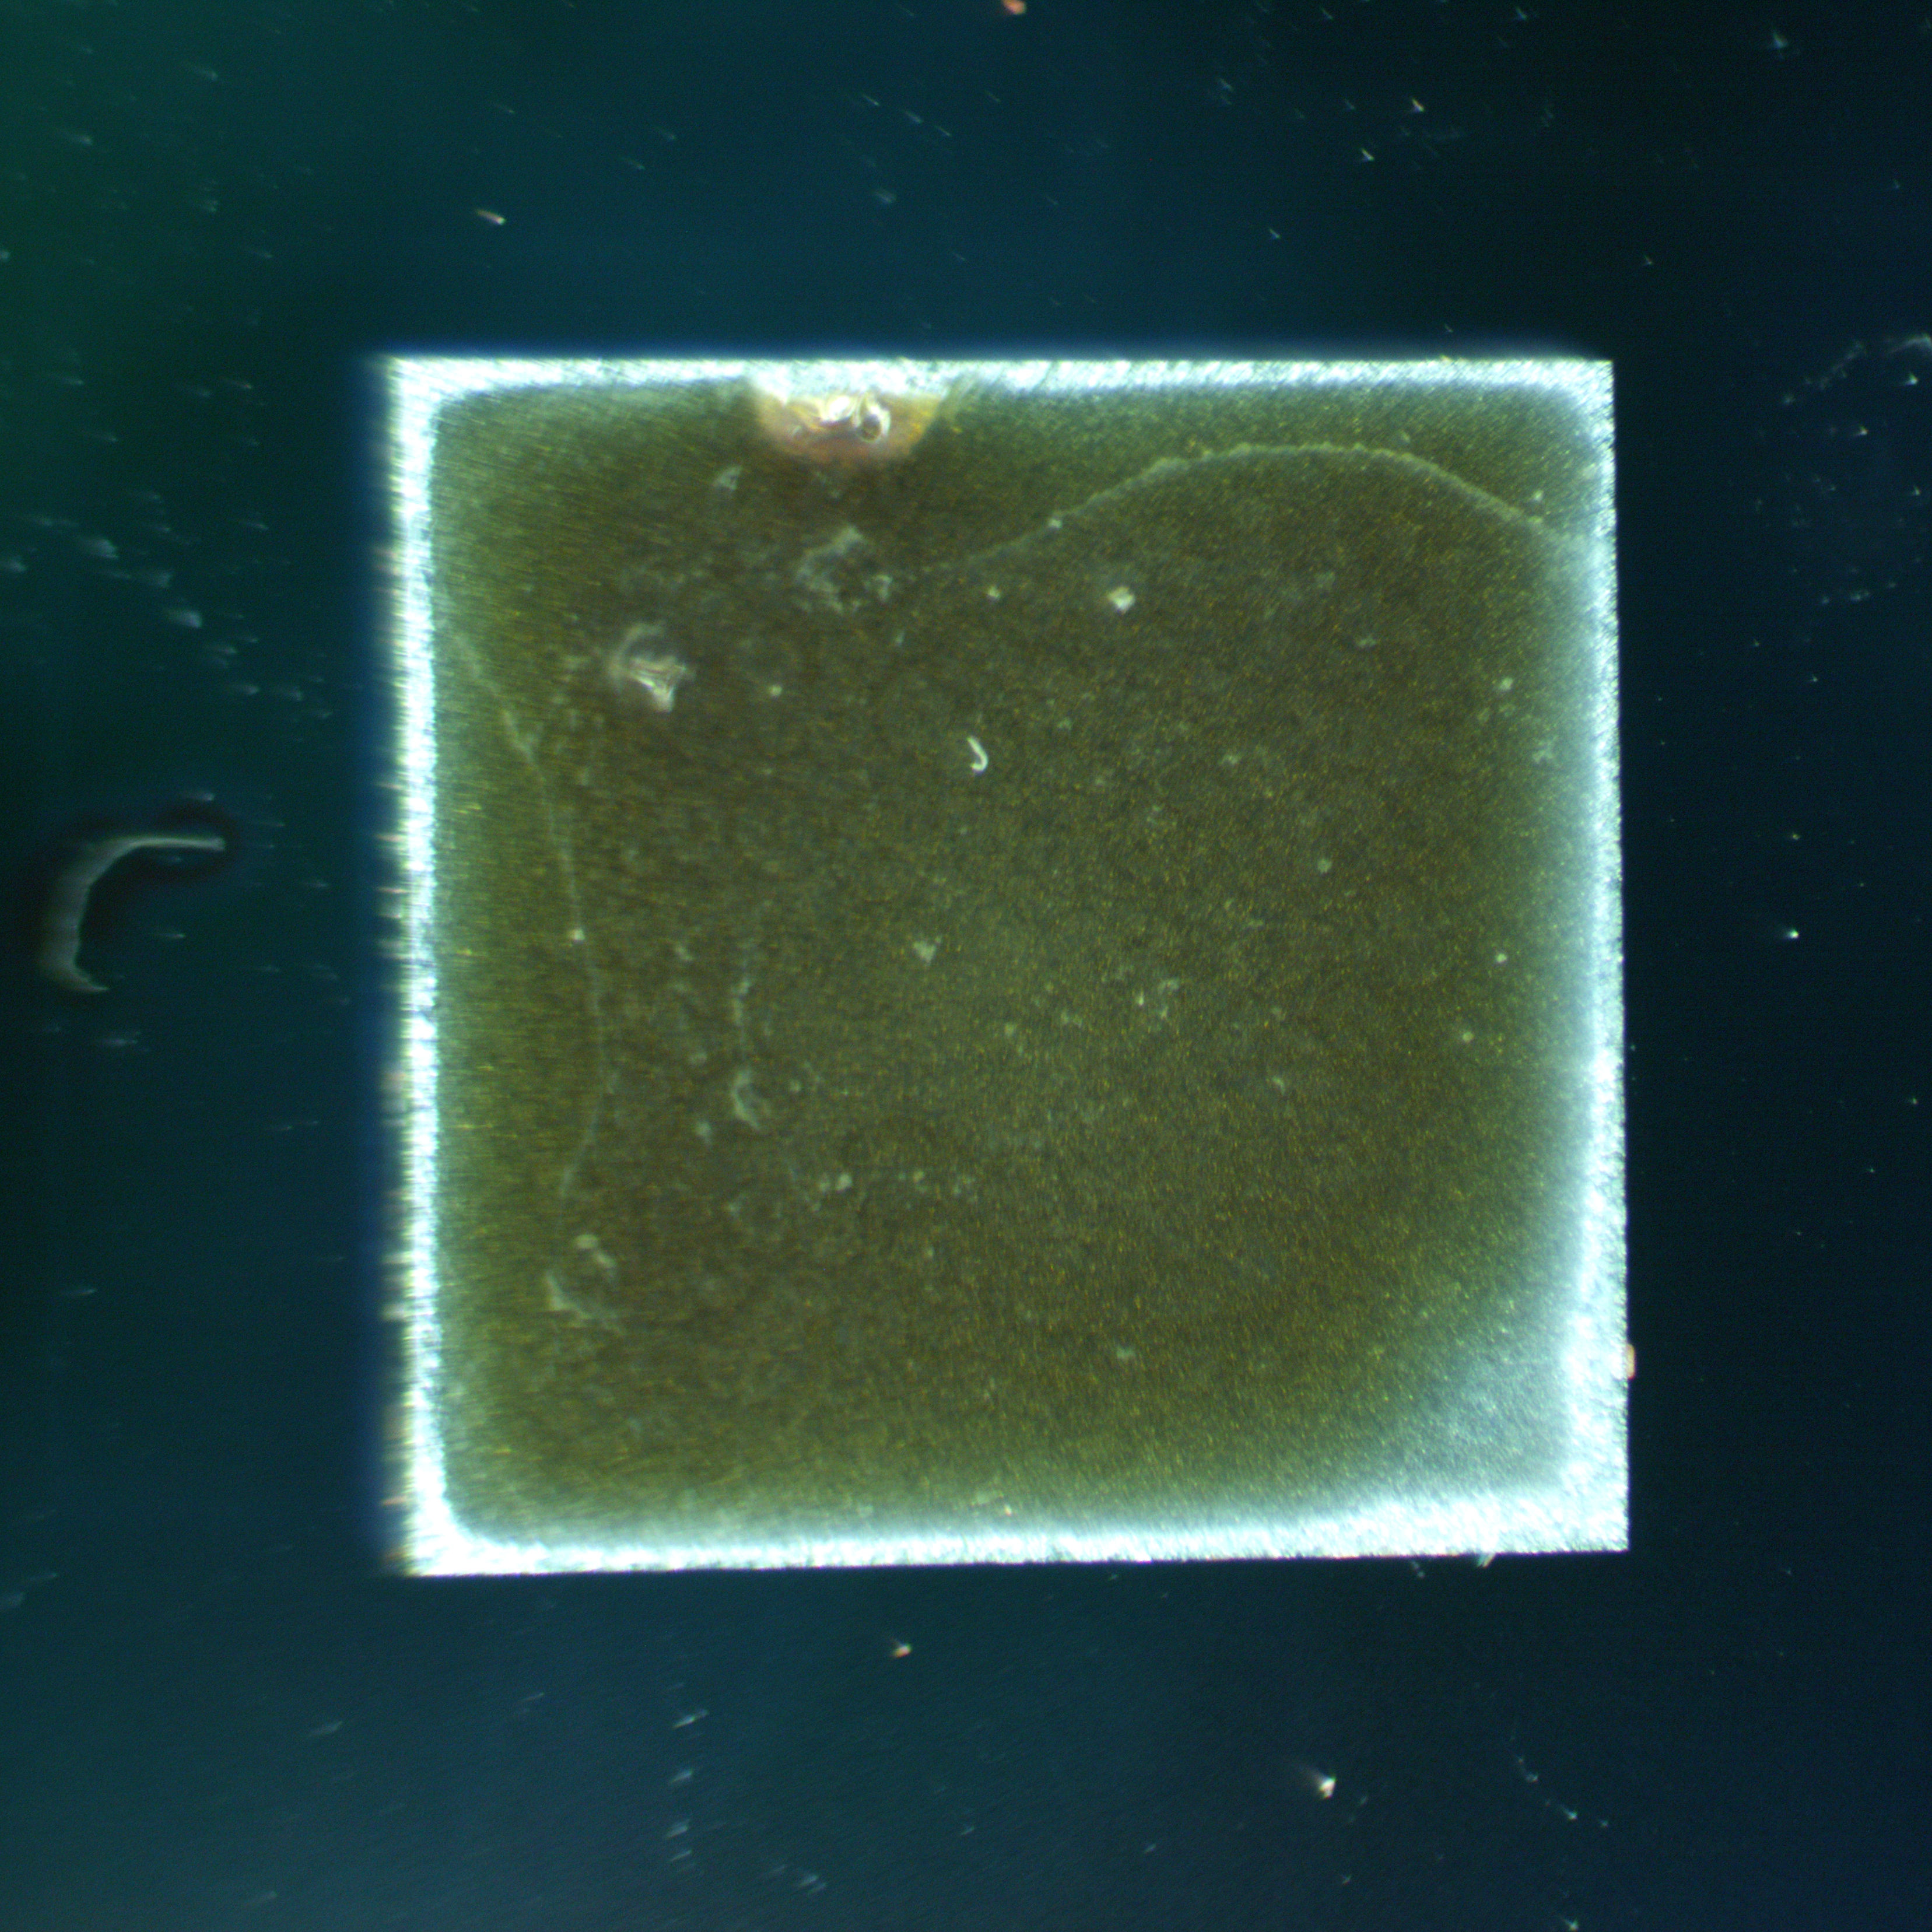
\includegraphics[width=\linewidth]{pics/spincoat/no7/7114.jpg}
        \caption{\textcolor{blue!60!black}{\textbf{Heater 9}}}
    \end{subfigure}

    \caption[Optical Images of the Heater in Passivation Test \#7]{Optical images of the nine Heater of the coating test \#7. The two heaters that could be removed from the glue are highlighted in blue and the height measurement was taken of those marked by a "*"}
    \label{fig:PT7}
\end{figure}
%================================================================================
%================================================================================
\begin{figure}[htbp]
    \centering

    % ---------- Row 1 ----------
    \begin{subfigure}[t]{0.3\textwidth}
        \centering
        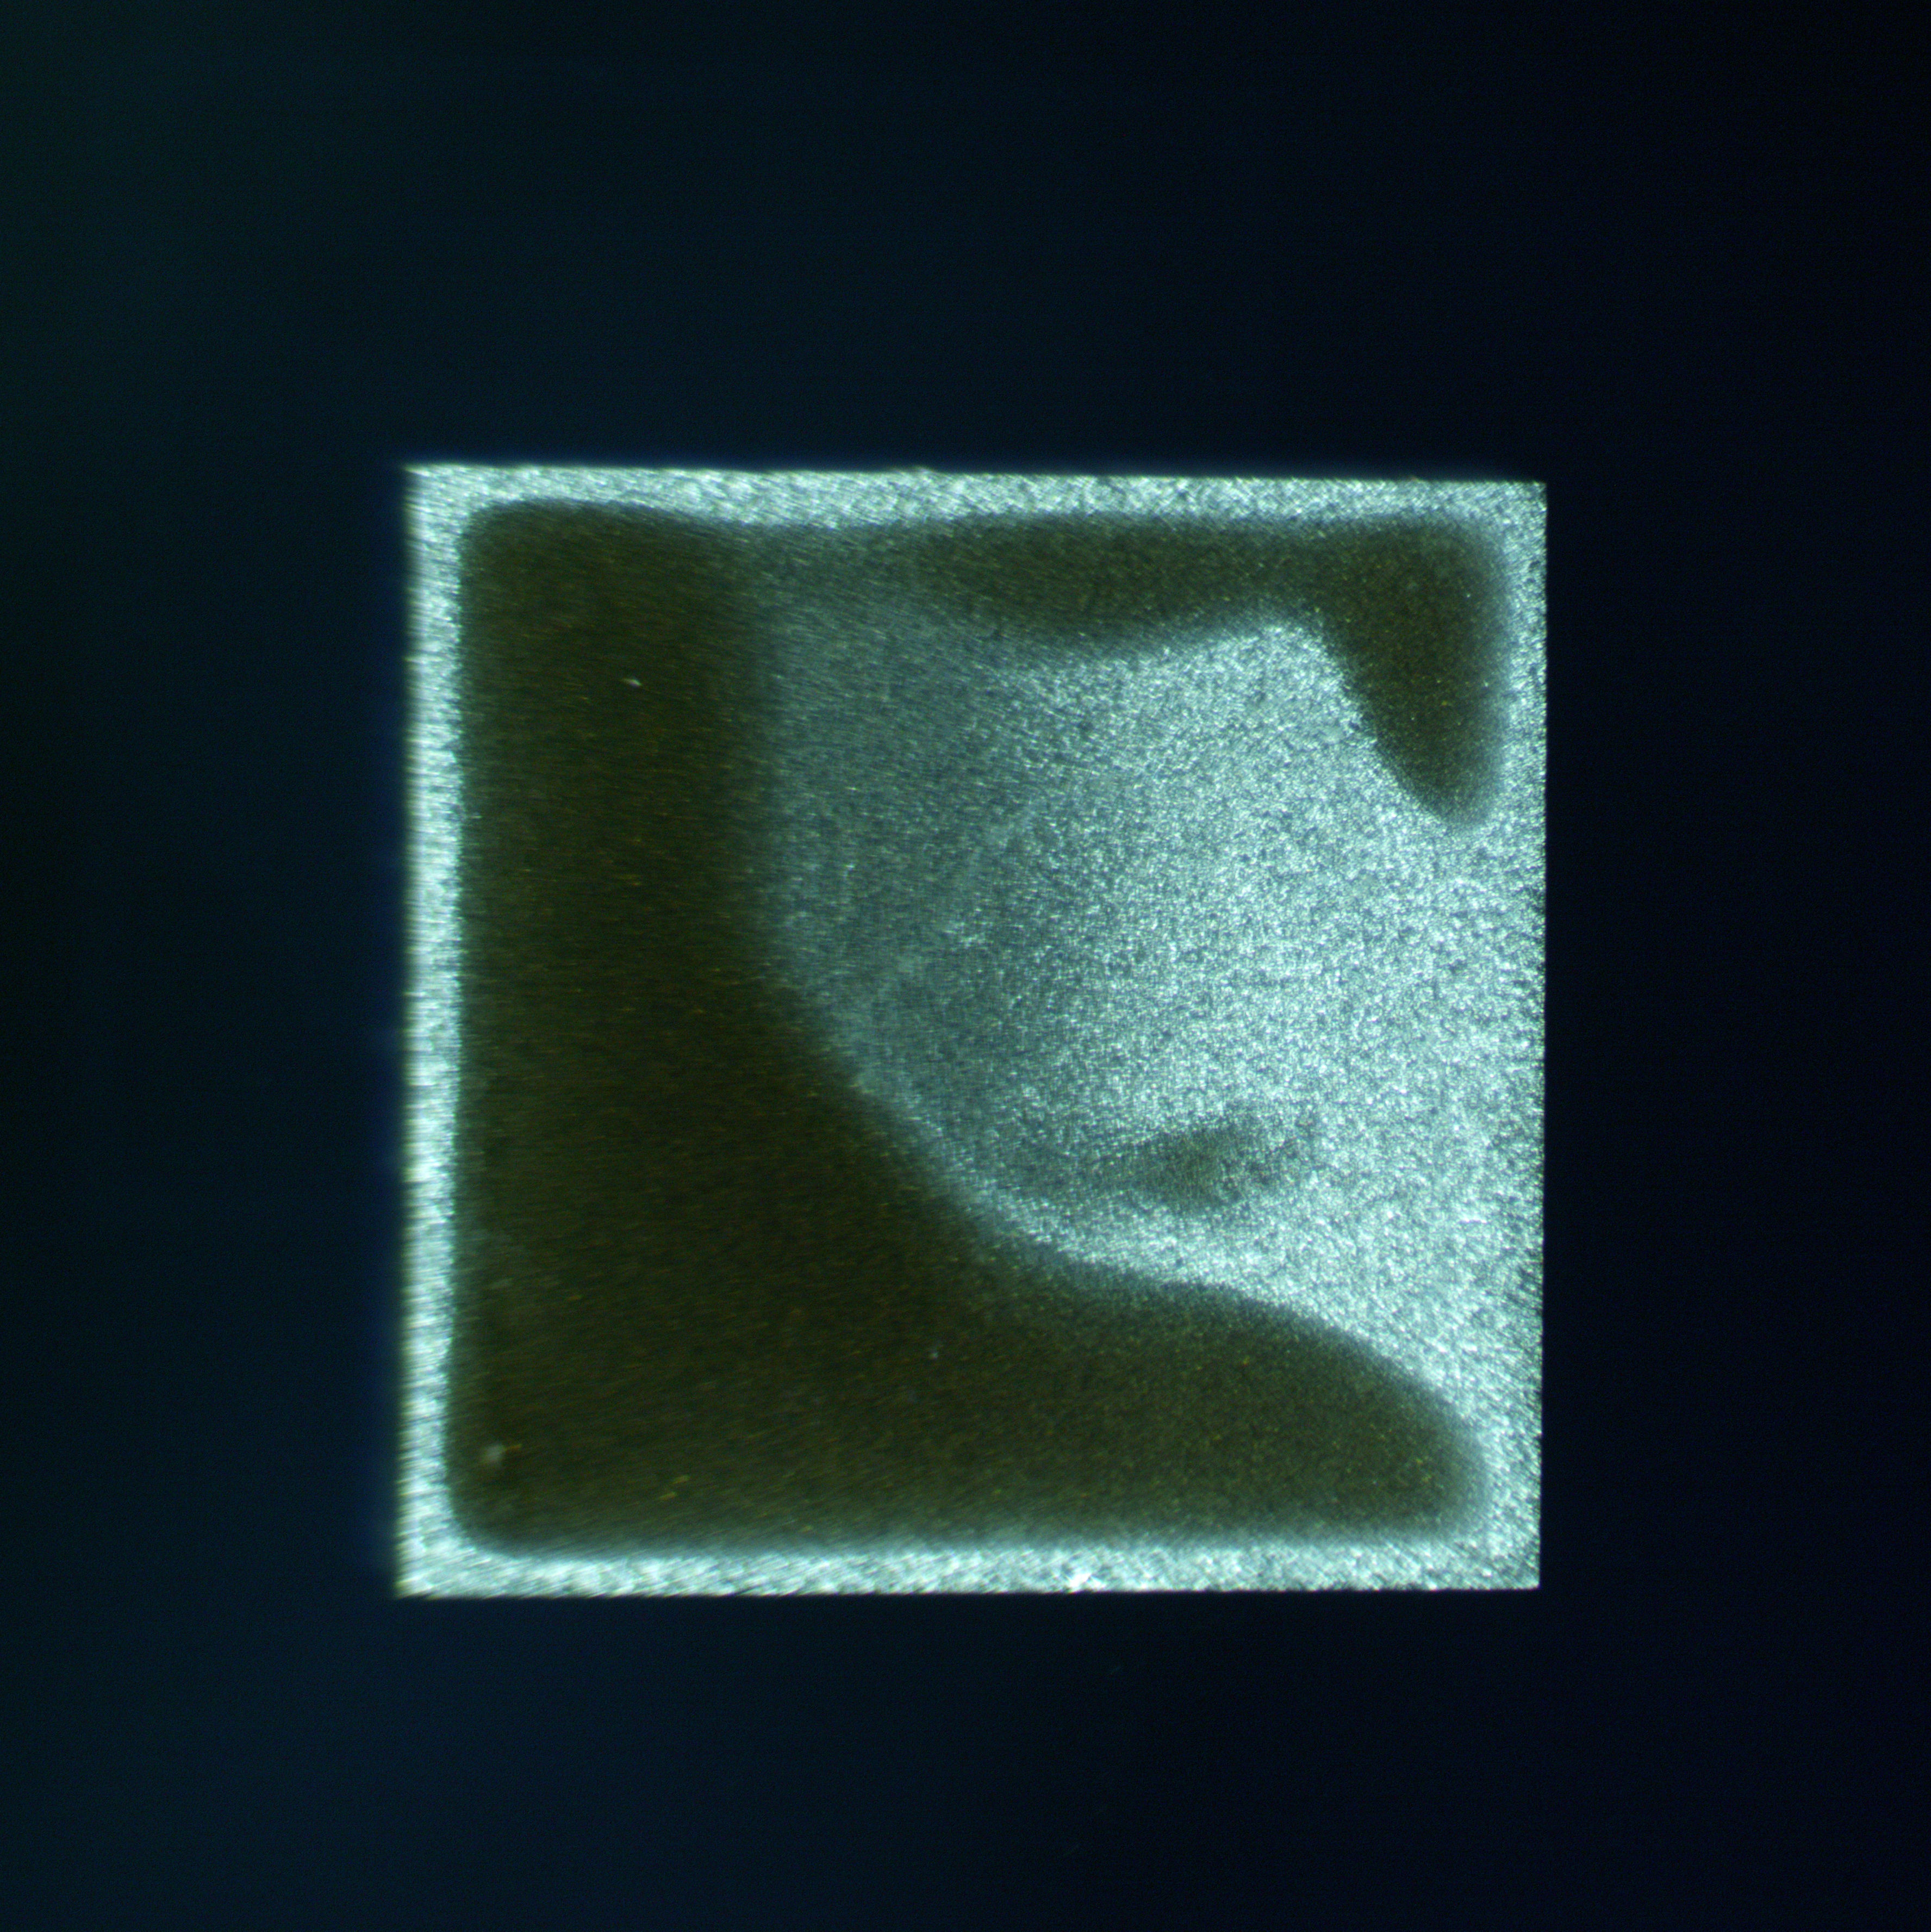
\includegraphics[width=\linewidth]{pics/spincoat/no8/8110.jpg}
        \caption{\textcolor{blue!60!black}{\textbf{Heater 1}}}
    \end{subfigure}
    \hfill
    \begin{subfigure}[t]{0.3\textwidth}
        \centering
        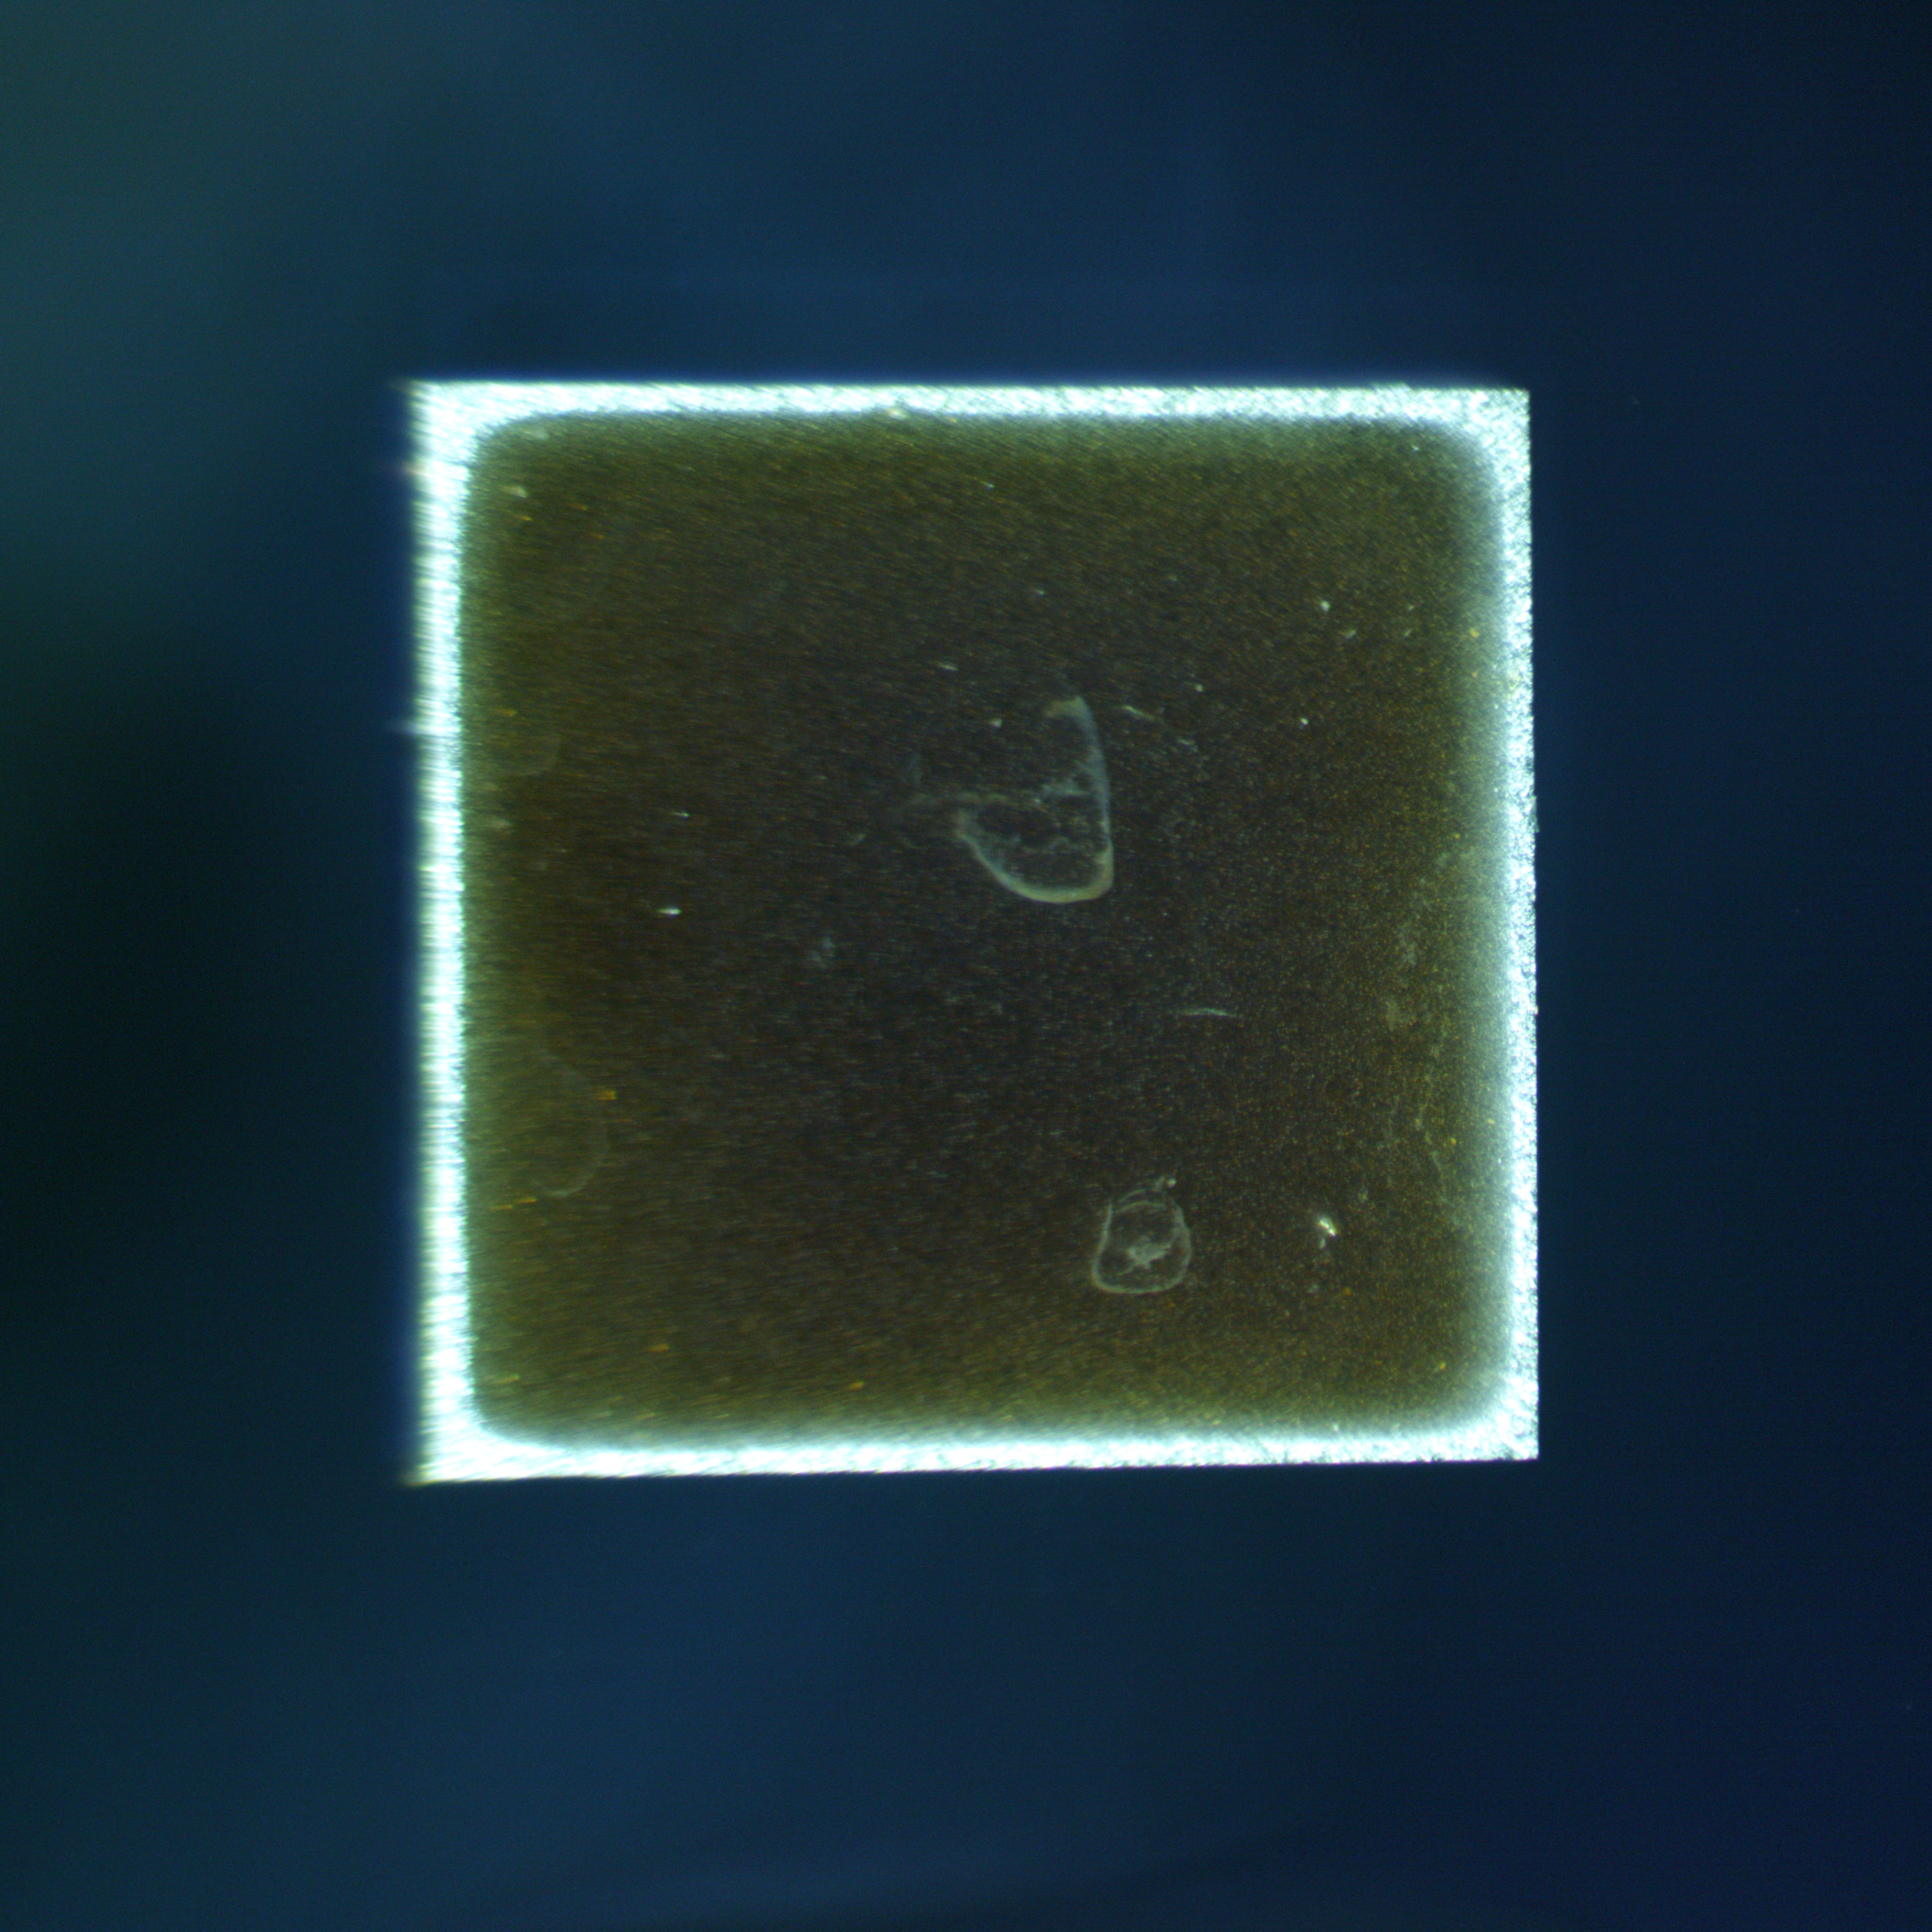
\includegraphics[width=\linewidth]{pics/spincoat/no8/8111.jpg}
        \caption{\textcolor{blue!60!black}{\textbf{Heater 2}}}
    \end{subfigure}
    \hfill
    \begin{subfigure}[t]{0.3\textwidth}
        \centering
        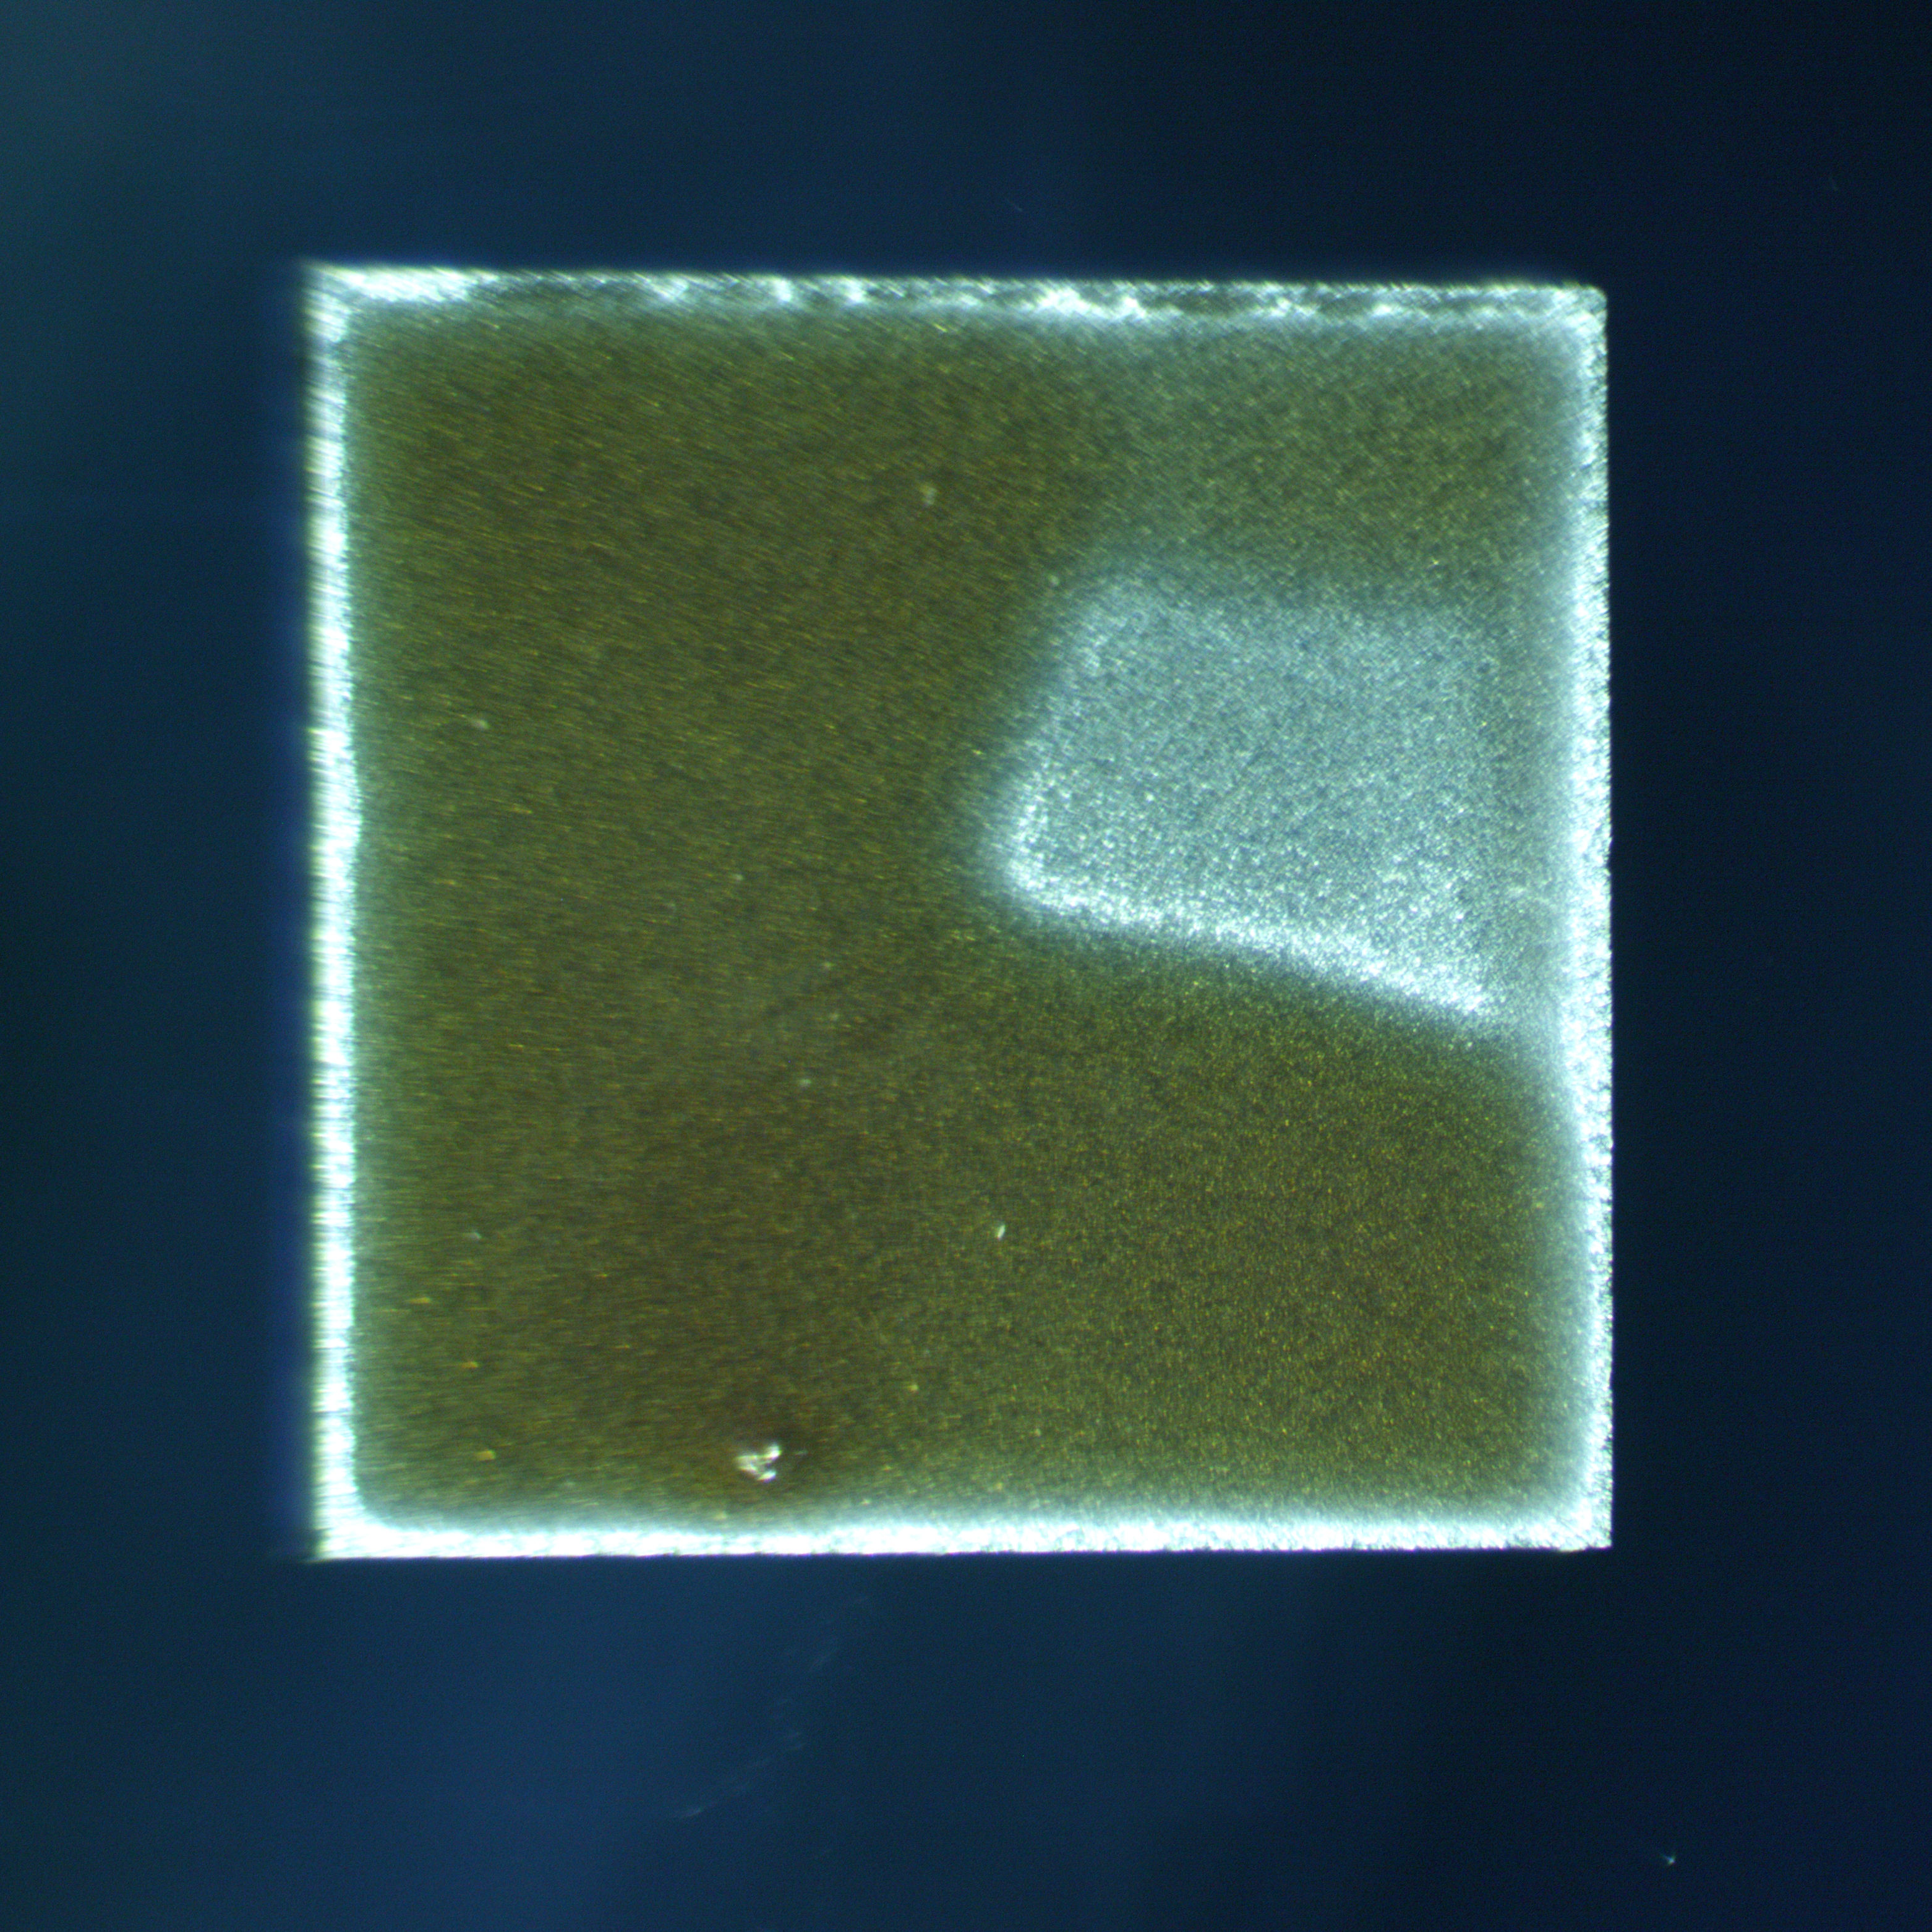
\includegraphics[width=\linewidth]{pics/spincoat/no8/8112.jpg}
        \caption{\textcolor{blue!60!black}{\textbf{Heater 3}}}
    \end{subfigure}

    \vspace{0.8cm}

    % ---------- Row 2 ----------
    \begin{subfigure}[t]{0.3\textwidth}
        \centering
        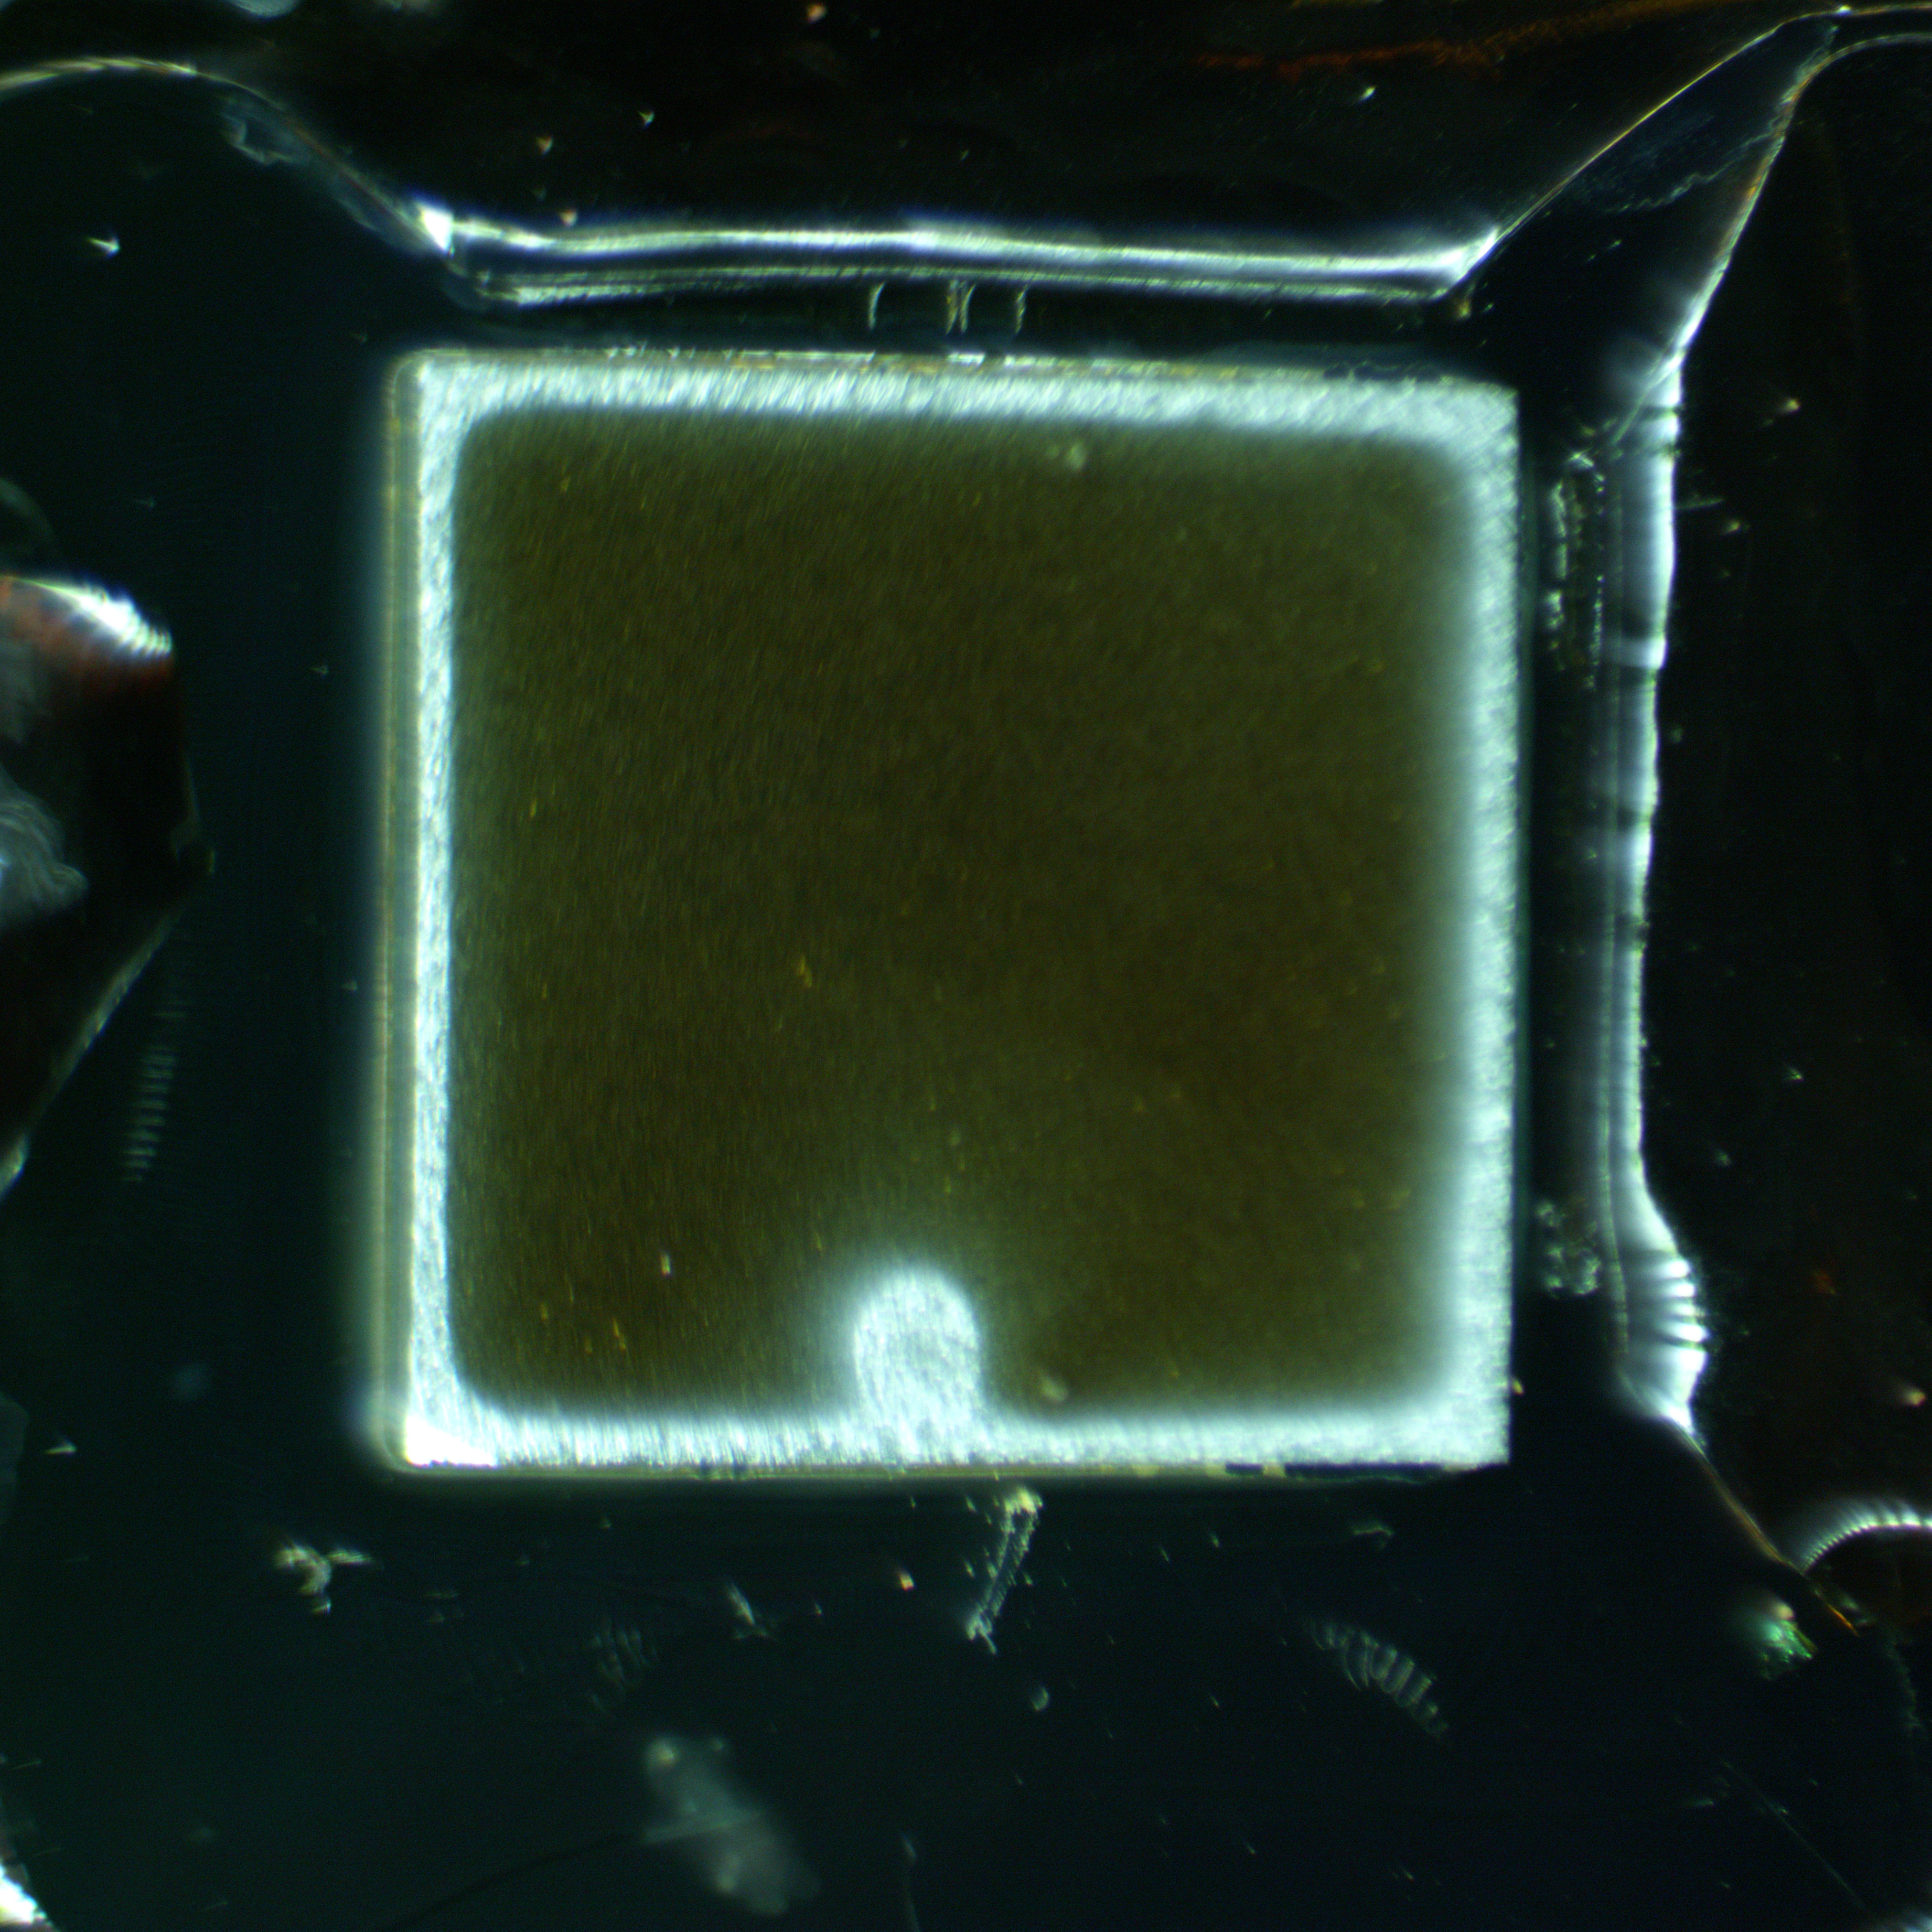
\includegraphics[width=\linewidth]{pics/spincoat/no8/8104.jpg}
        \caption{Heater 4}
    \end{subfigure}
    \hfill
    \begin{subfigure}[t]{0.3\textwidth}
        \centering
        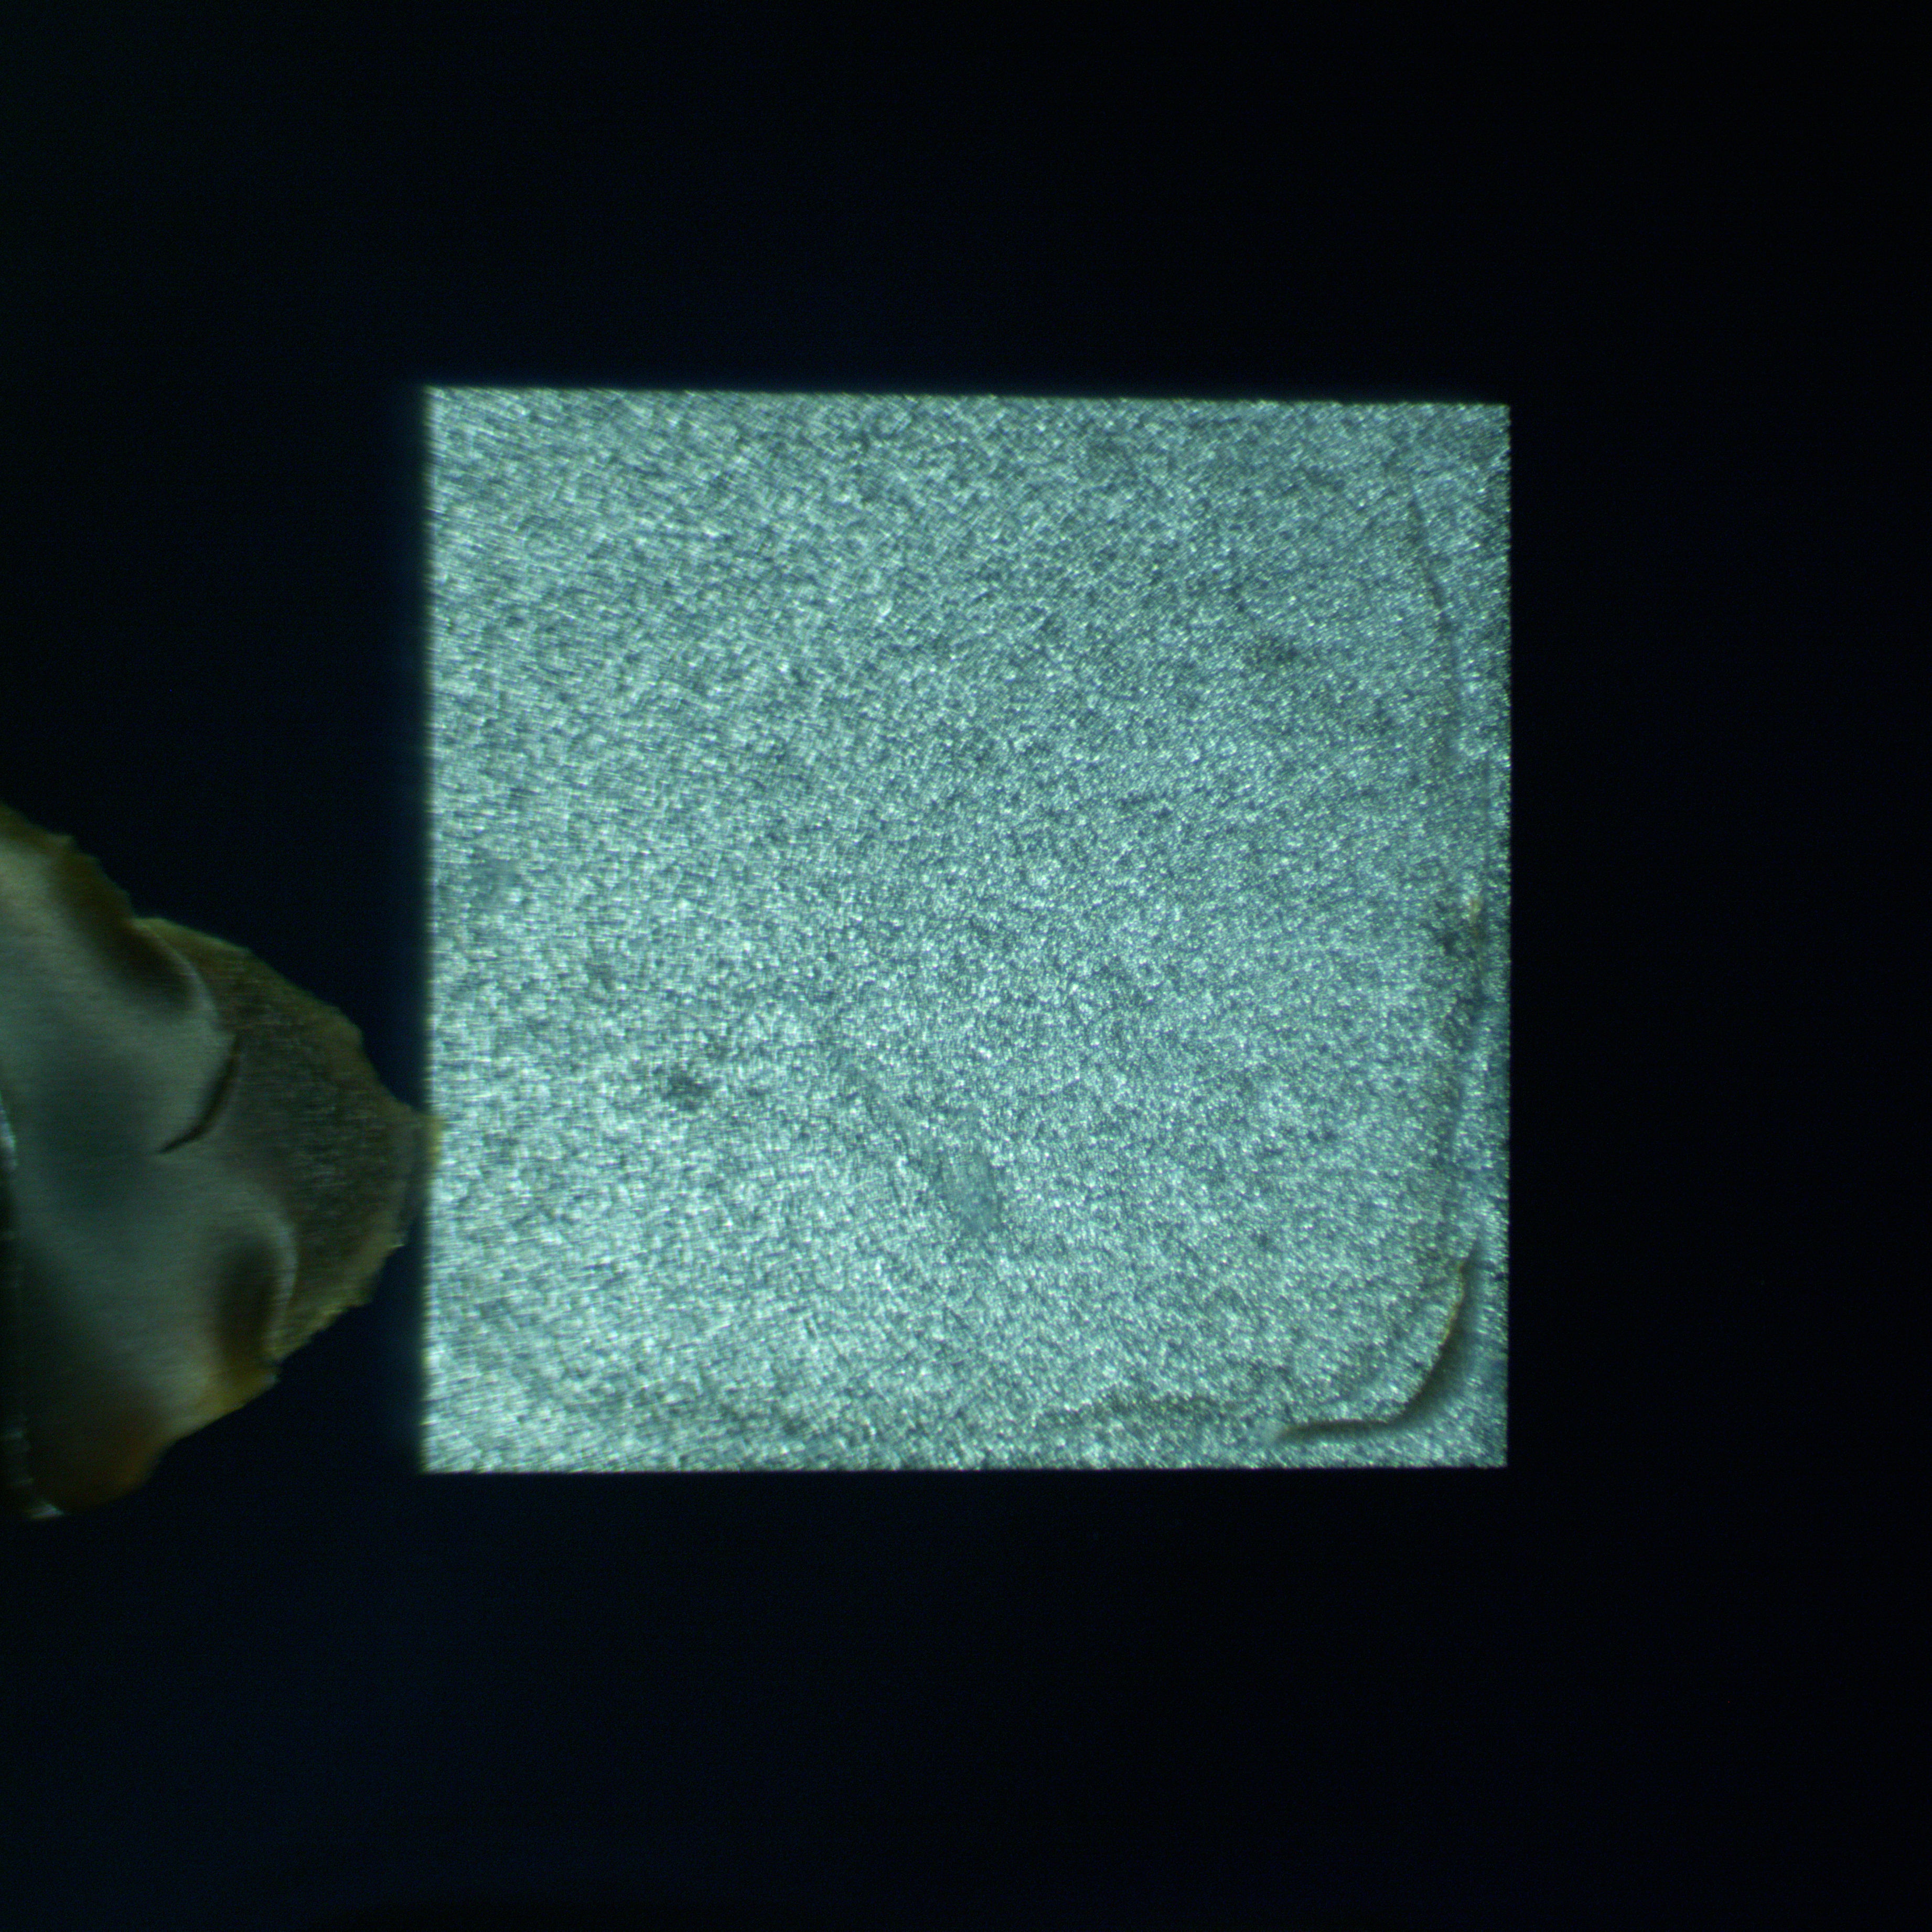
\includegraphics[width=\linewidth]{pics/spincoat/no8/8113.jpg}
        \caption{\textcolor{blue!60!black}{\textbf{Heater 5}}}
    \end{subfigure}
    \hfill
    \begin{subfigure}[t]{0.3\textwidth}
        \centering
        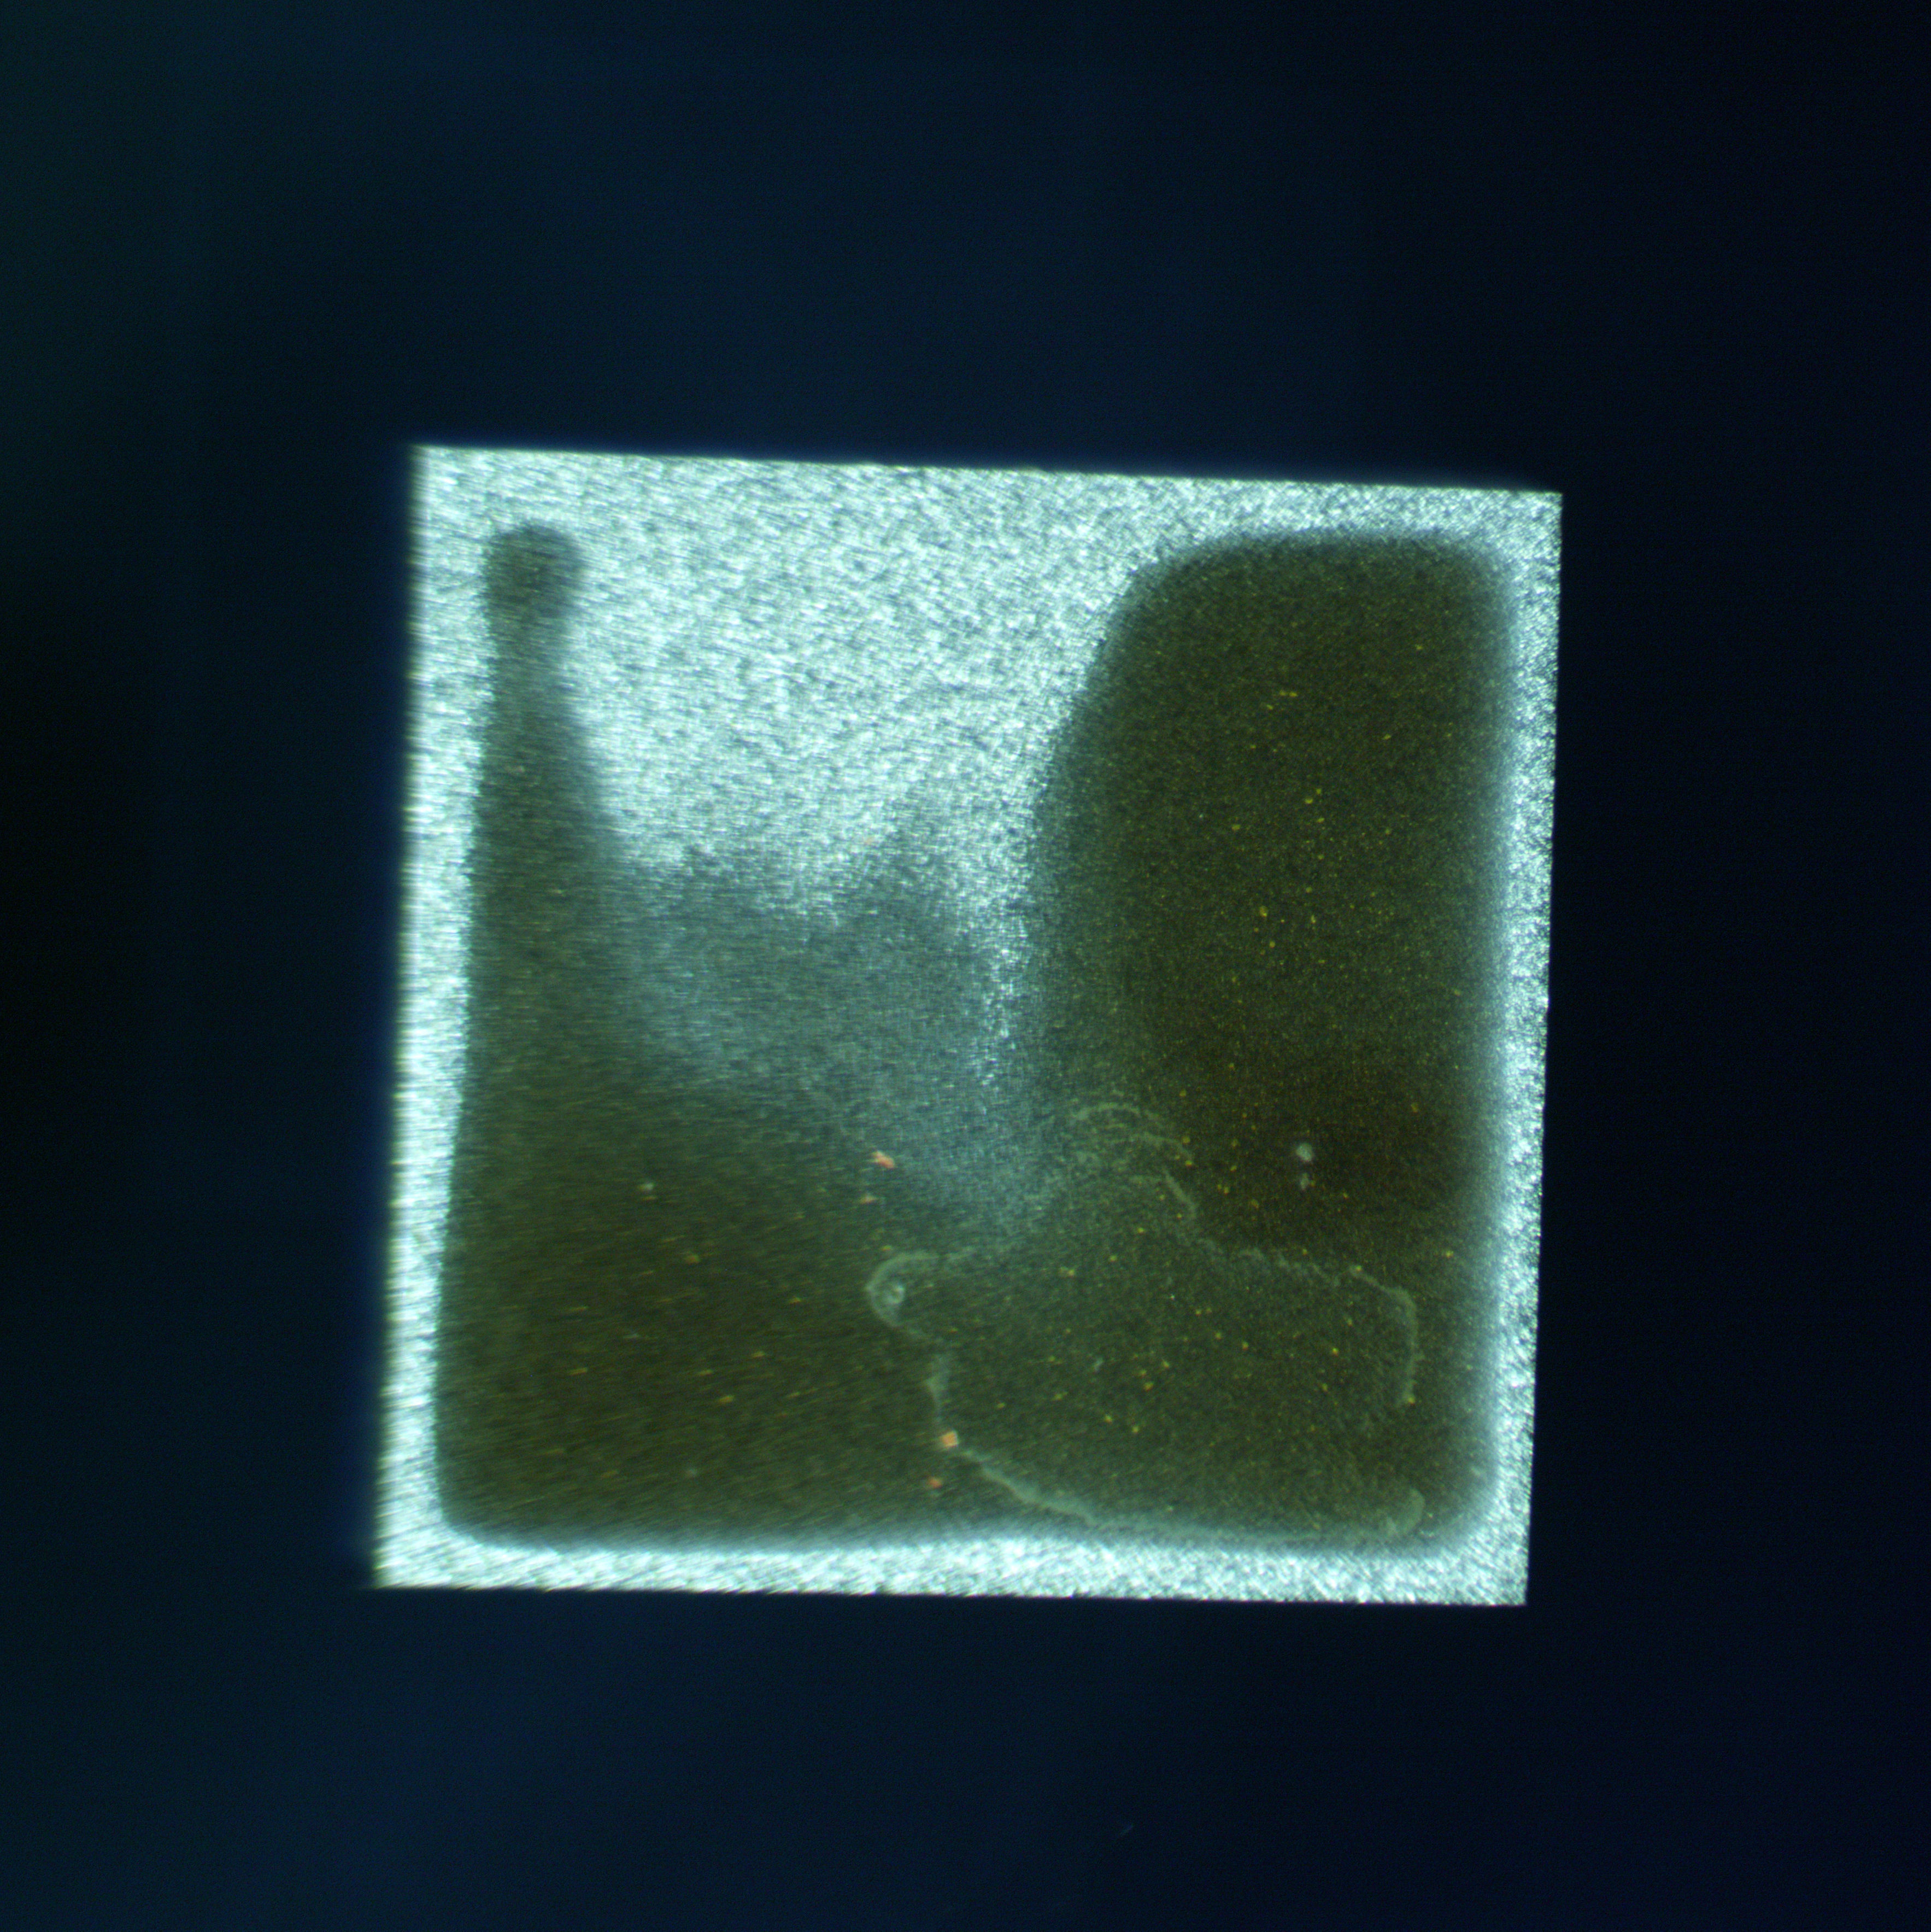
\includegraphics[width=\linewidth]{pics/spincoat/no8/8114.jpg}
        \caption{\textcolor{blue!60!black}{\textbf{Heater 6}}}
    \end{subfigure}

    \vspace{0.8cm}

    % ---------- Row 3 ----------
    \begin{subfigure}[t]{0.3\textwidth}
        \centering
        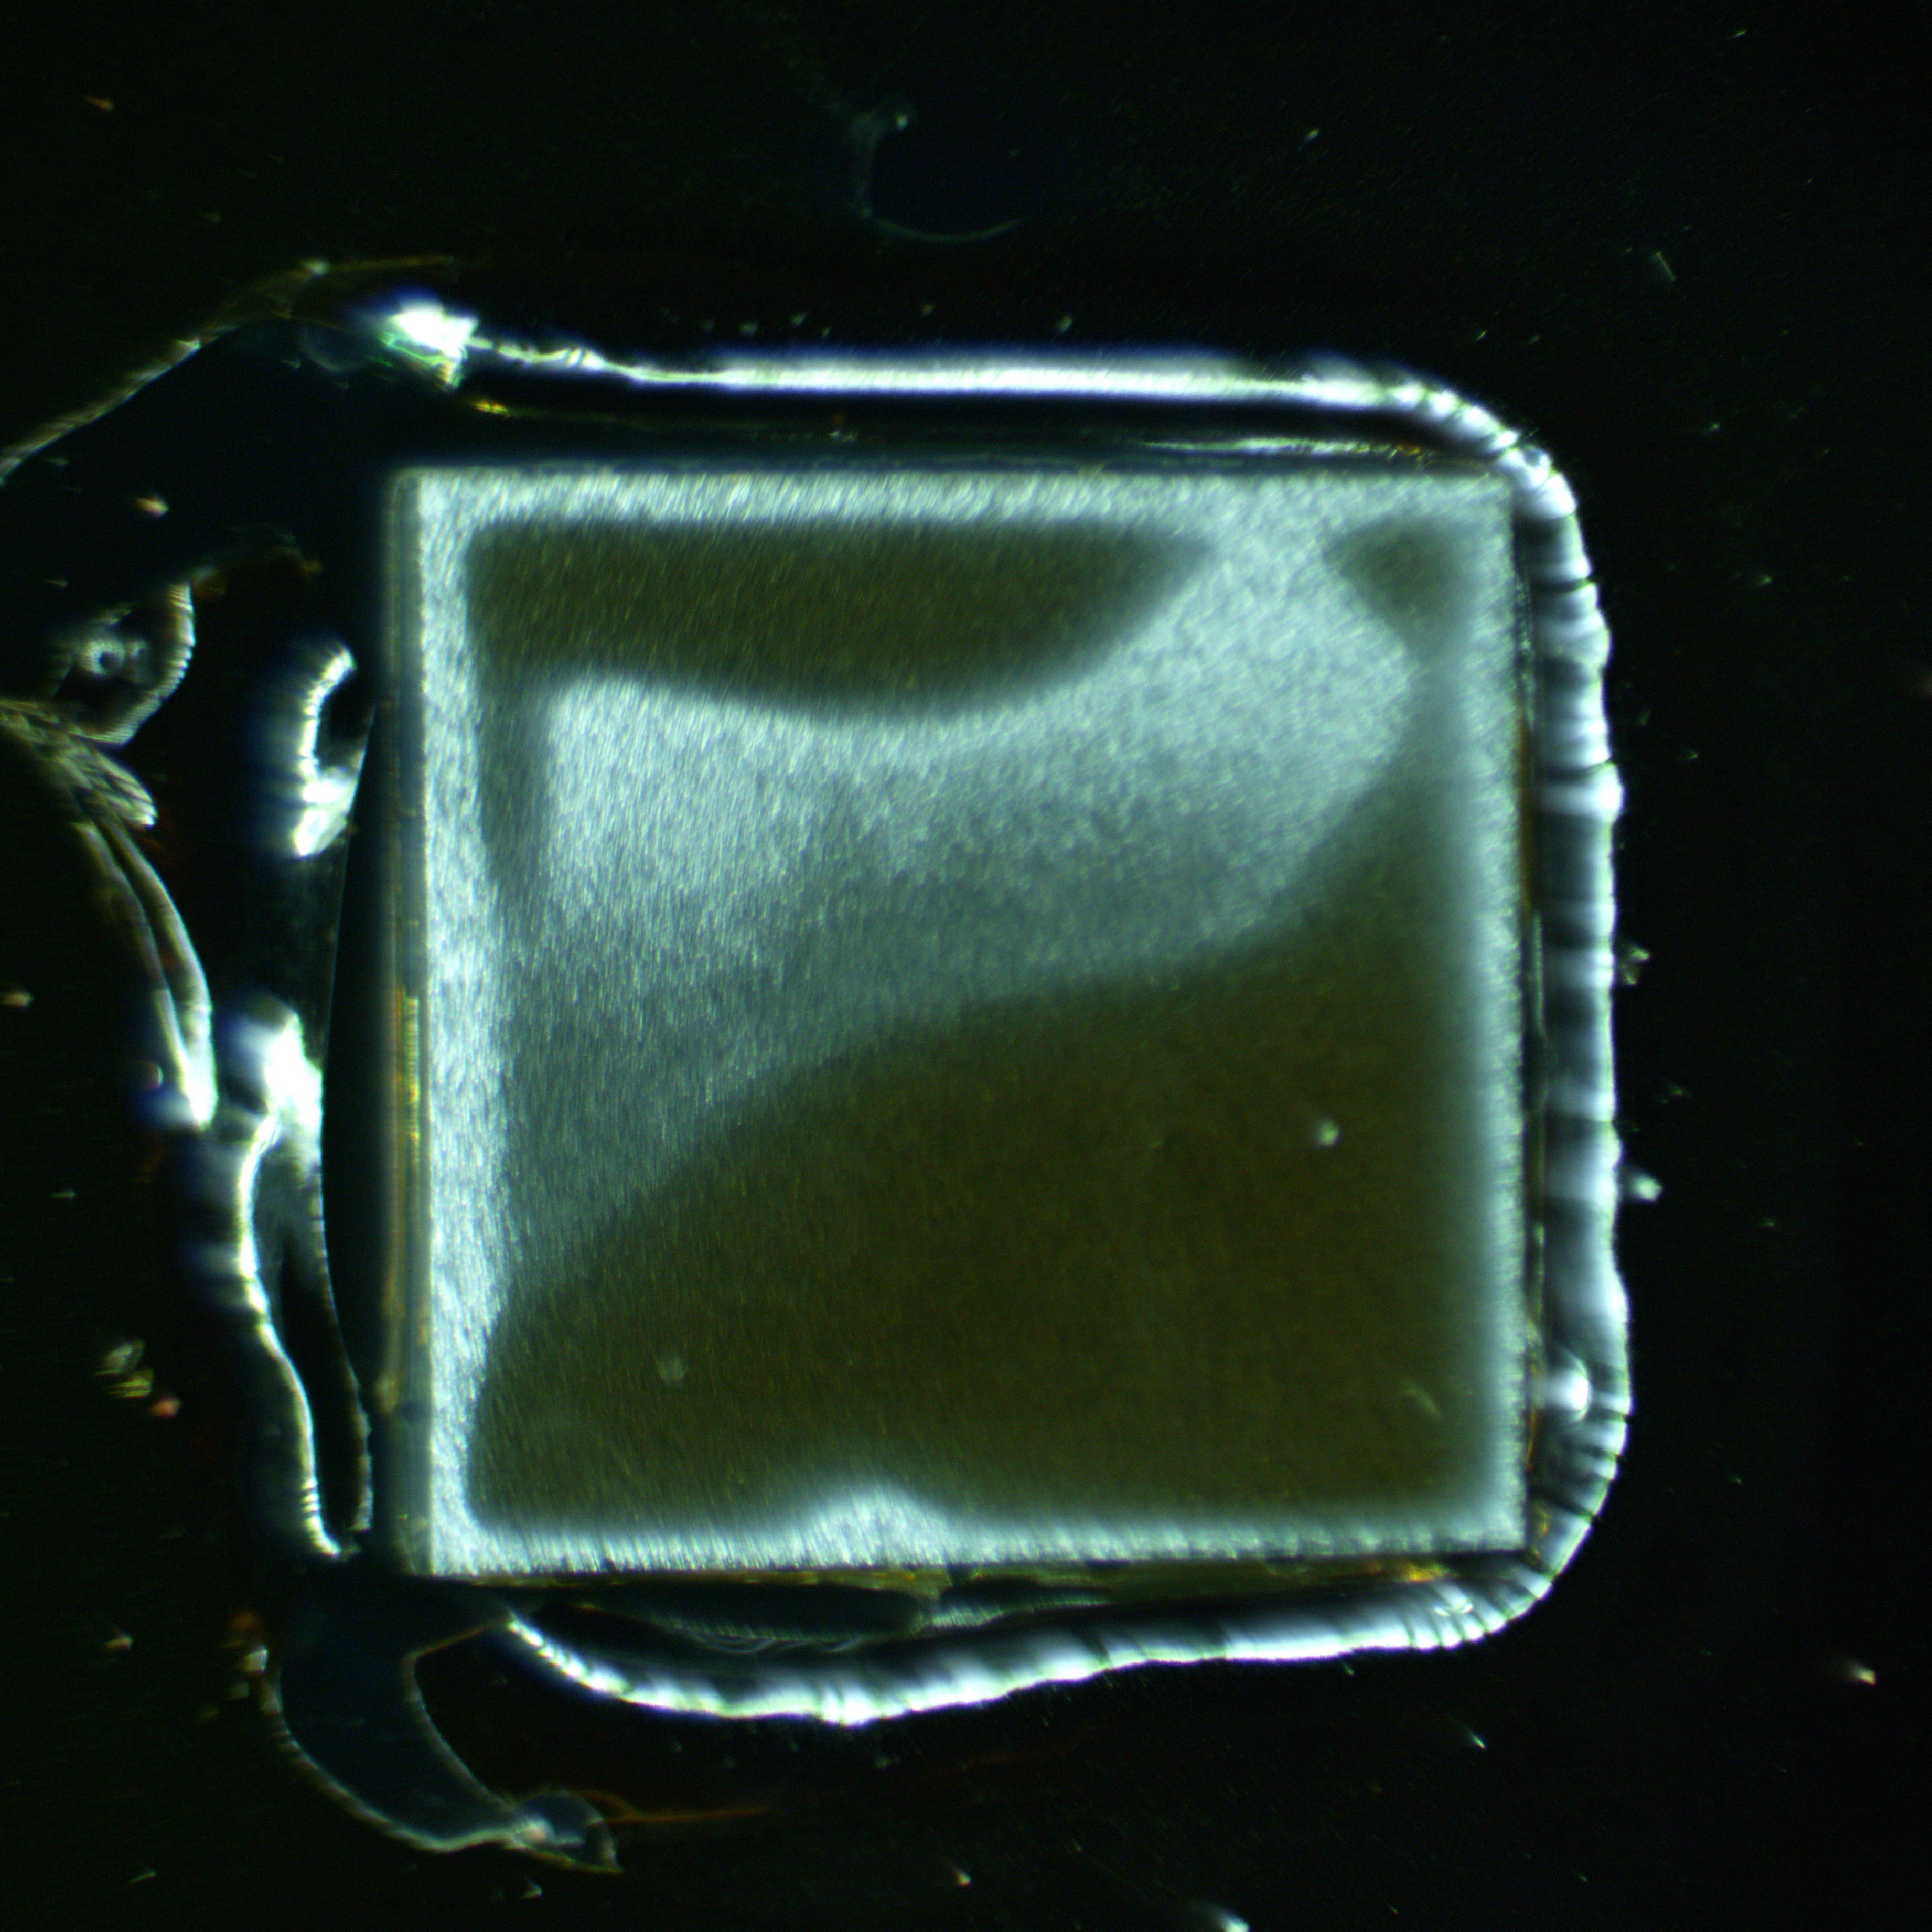
\includegraphics[width=\linewidth]{pics/spincoat/no8/8107.jpg}
        \caption{Heater 7}
    \end{subfigure}
    \hfill
    \begin{subfigure}[t]{0.3\textwidth}
        \centering
        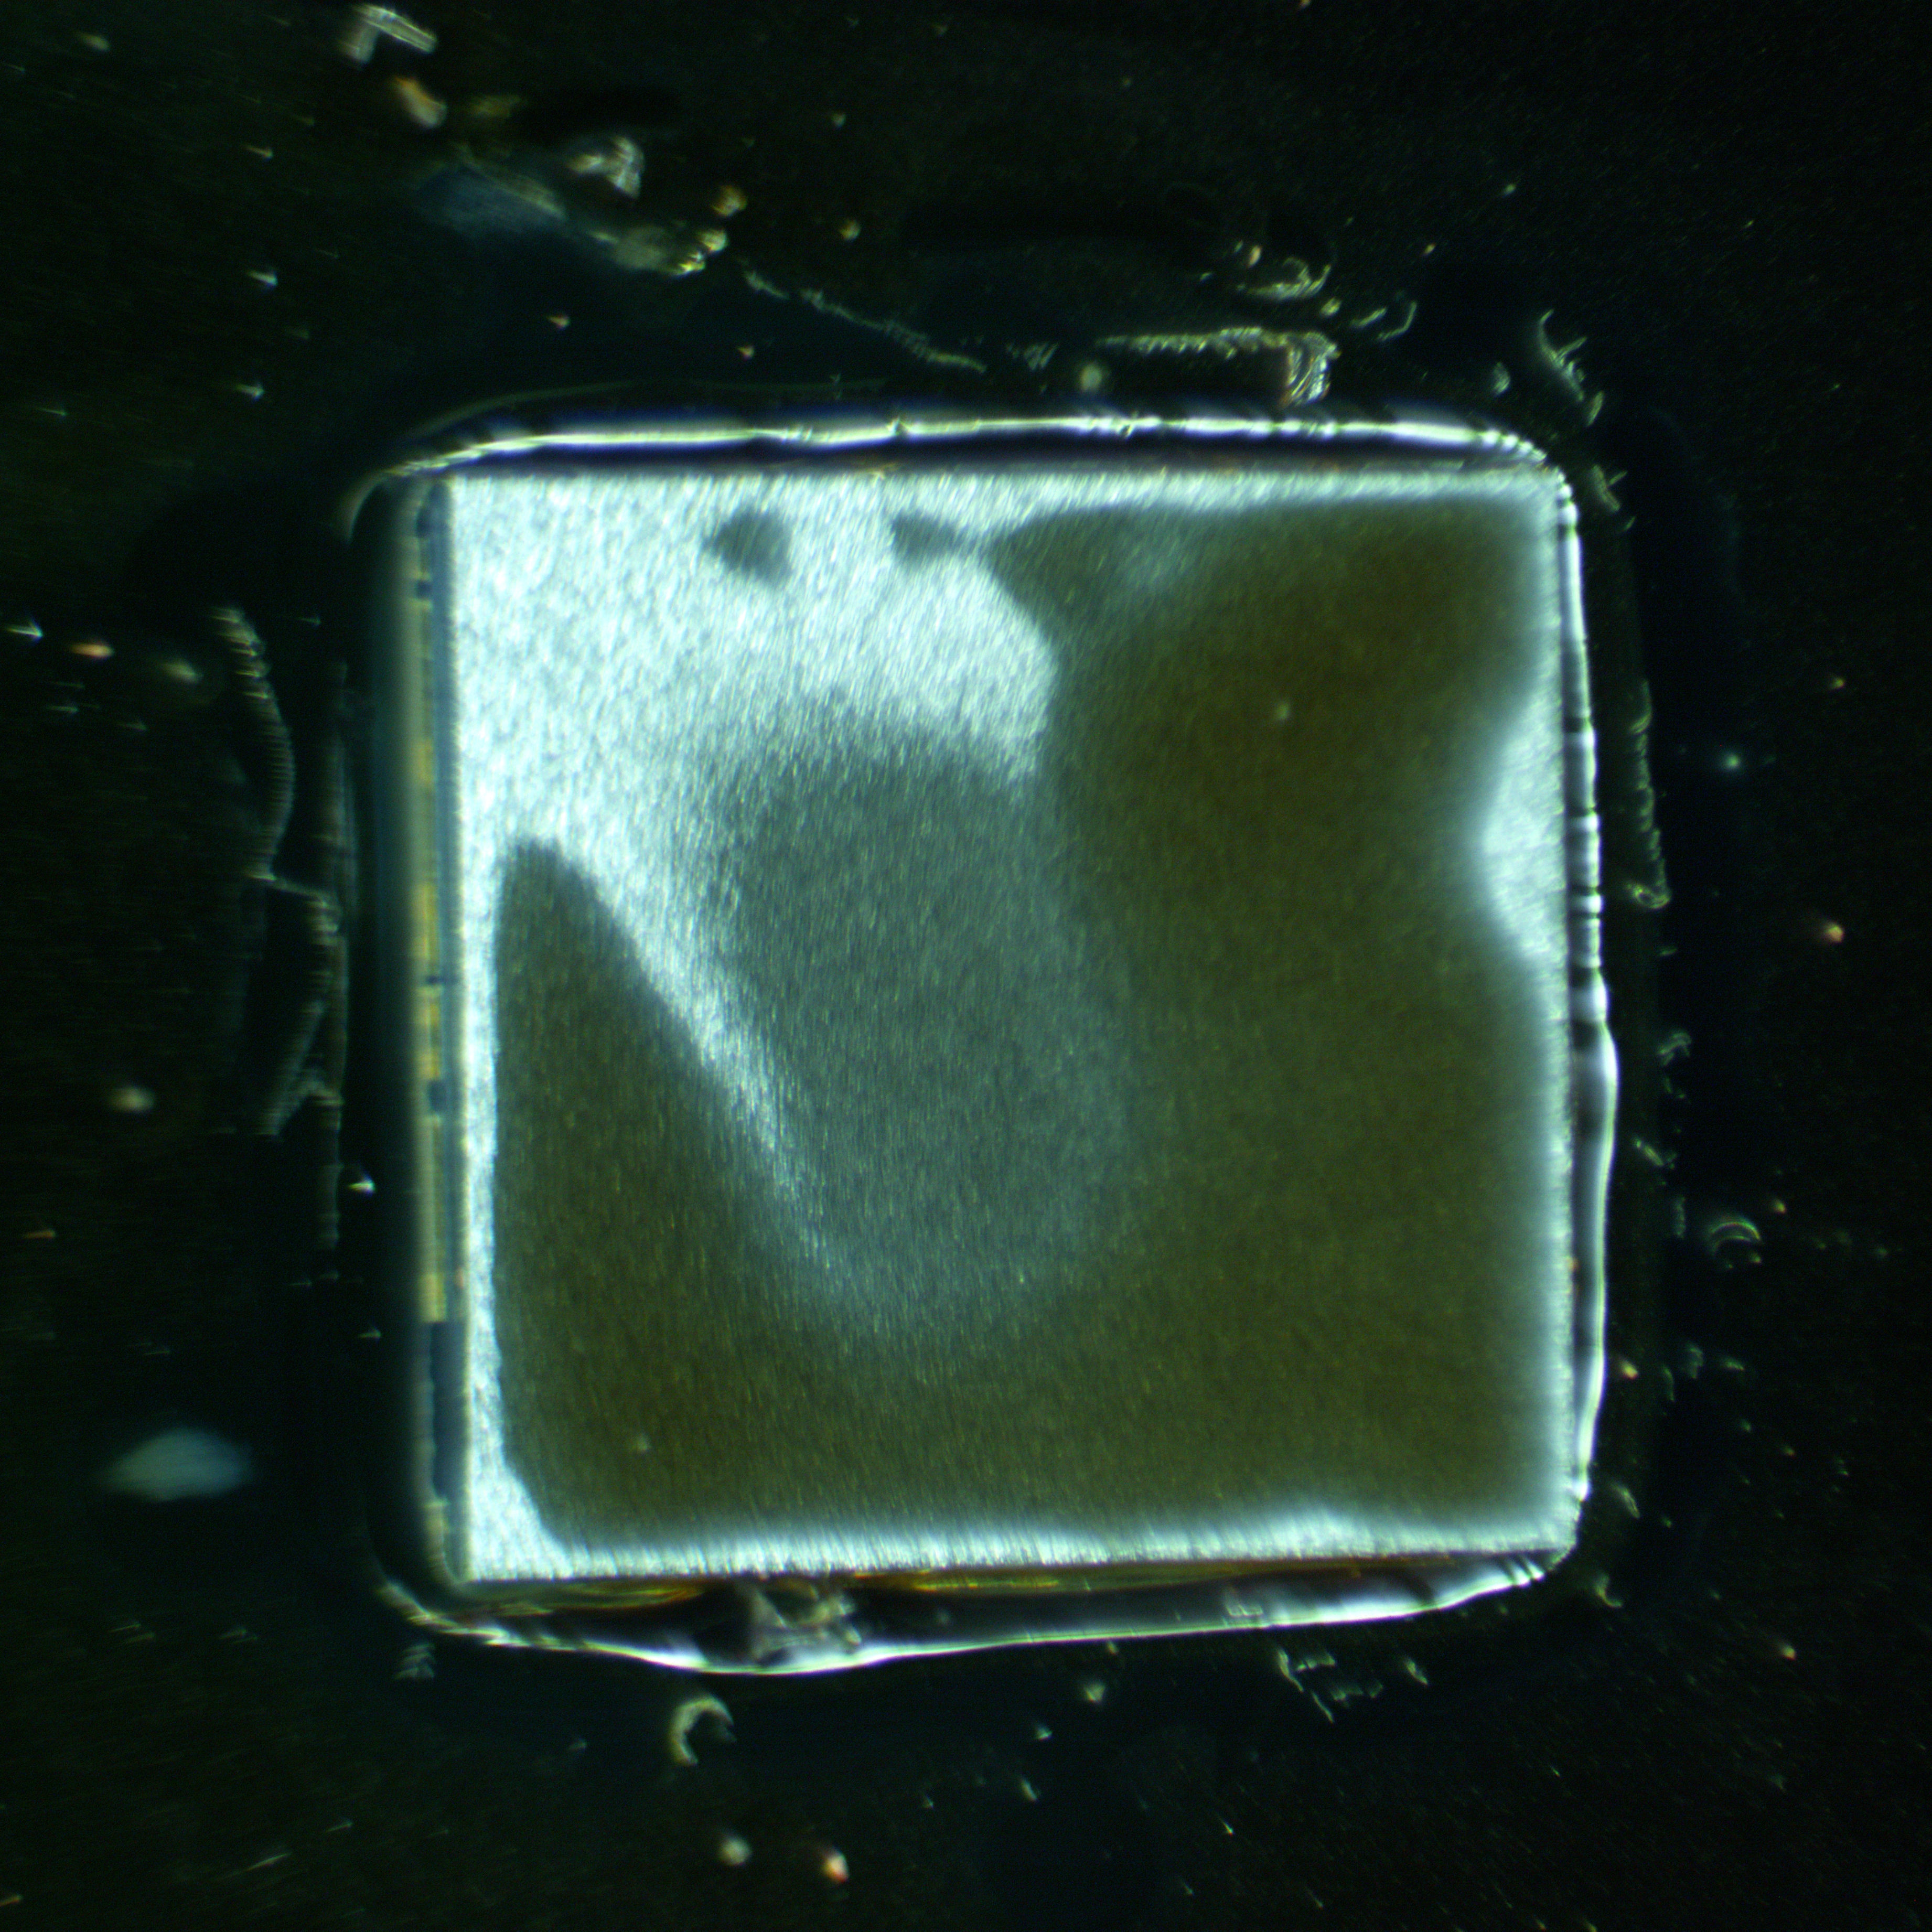
\includegraphics[width=\linewidth]{pics/spincoat/no8/8108.jpg}
        \caption{Heater 8}
    \end{subfigure}
    \hfill
    \begin{subfigure}[t]{0.3\textwidth}
        \centering
        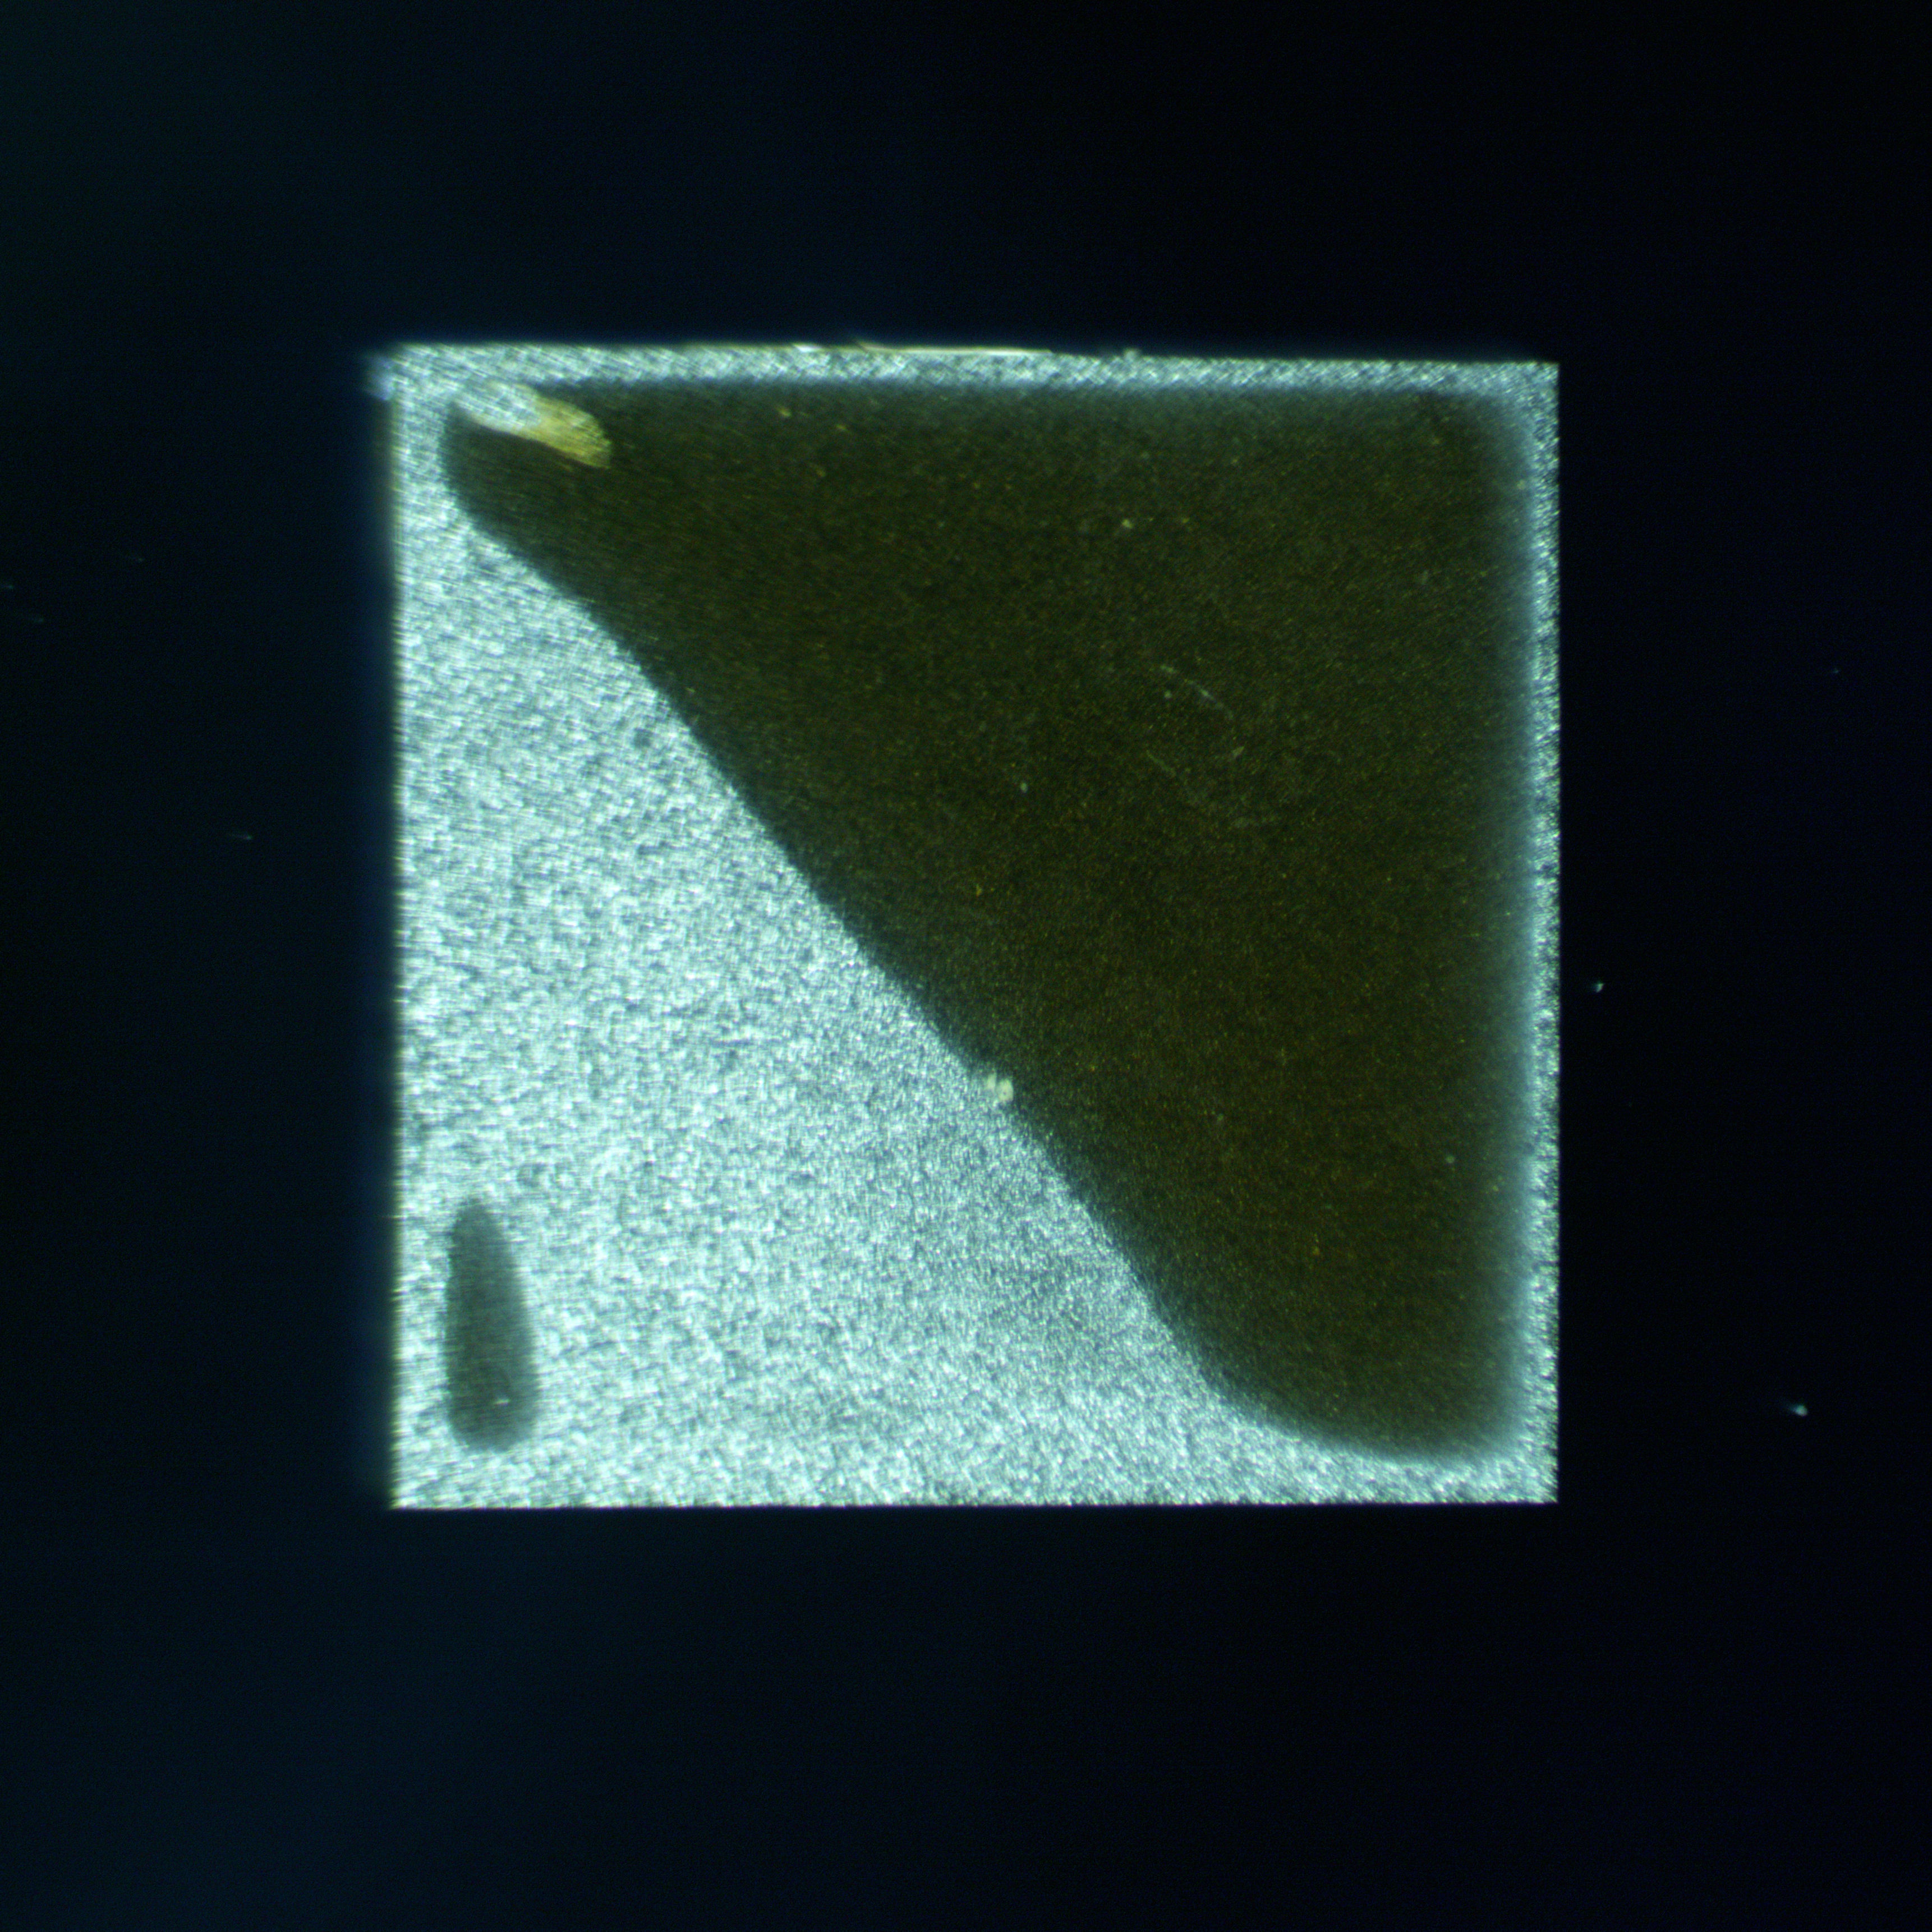
\includegraphics[width=\linewidth]{pics/spincoat/no8/8115.jpg}
        \caption{\textcolor{blue!60!black}{\textbf{Heater 9}}}
    \end{subfigure}

    \caption[Optical Images of the Heater in Passivation Test \#8]{Optical images of the nine Heater of the coating test \#8. The two heaters that could be removed from the glue are highlighted in blue and the height measurement was taken of those marked by a "*"}
    \label{fig:PT8}
\end{figure}
%================================================================================
%================================================================================
\begin{figure}[htbp]
    \centering

    % ---------- Row 1 ----------
    \begin{subfigure}[t]{0.3\textwidth}
        \centering
        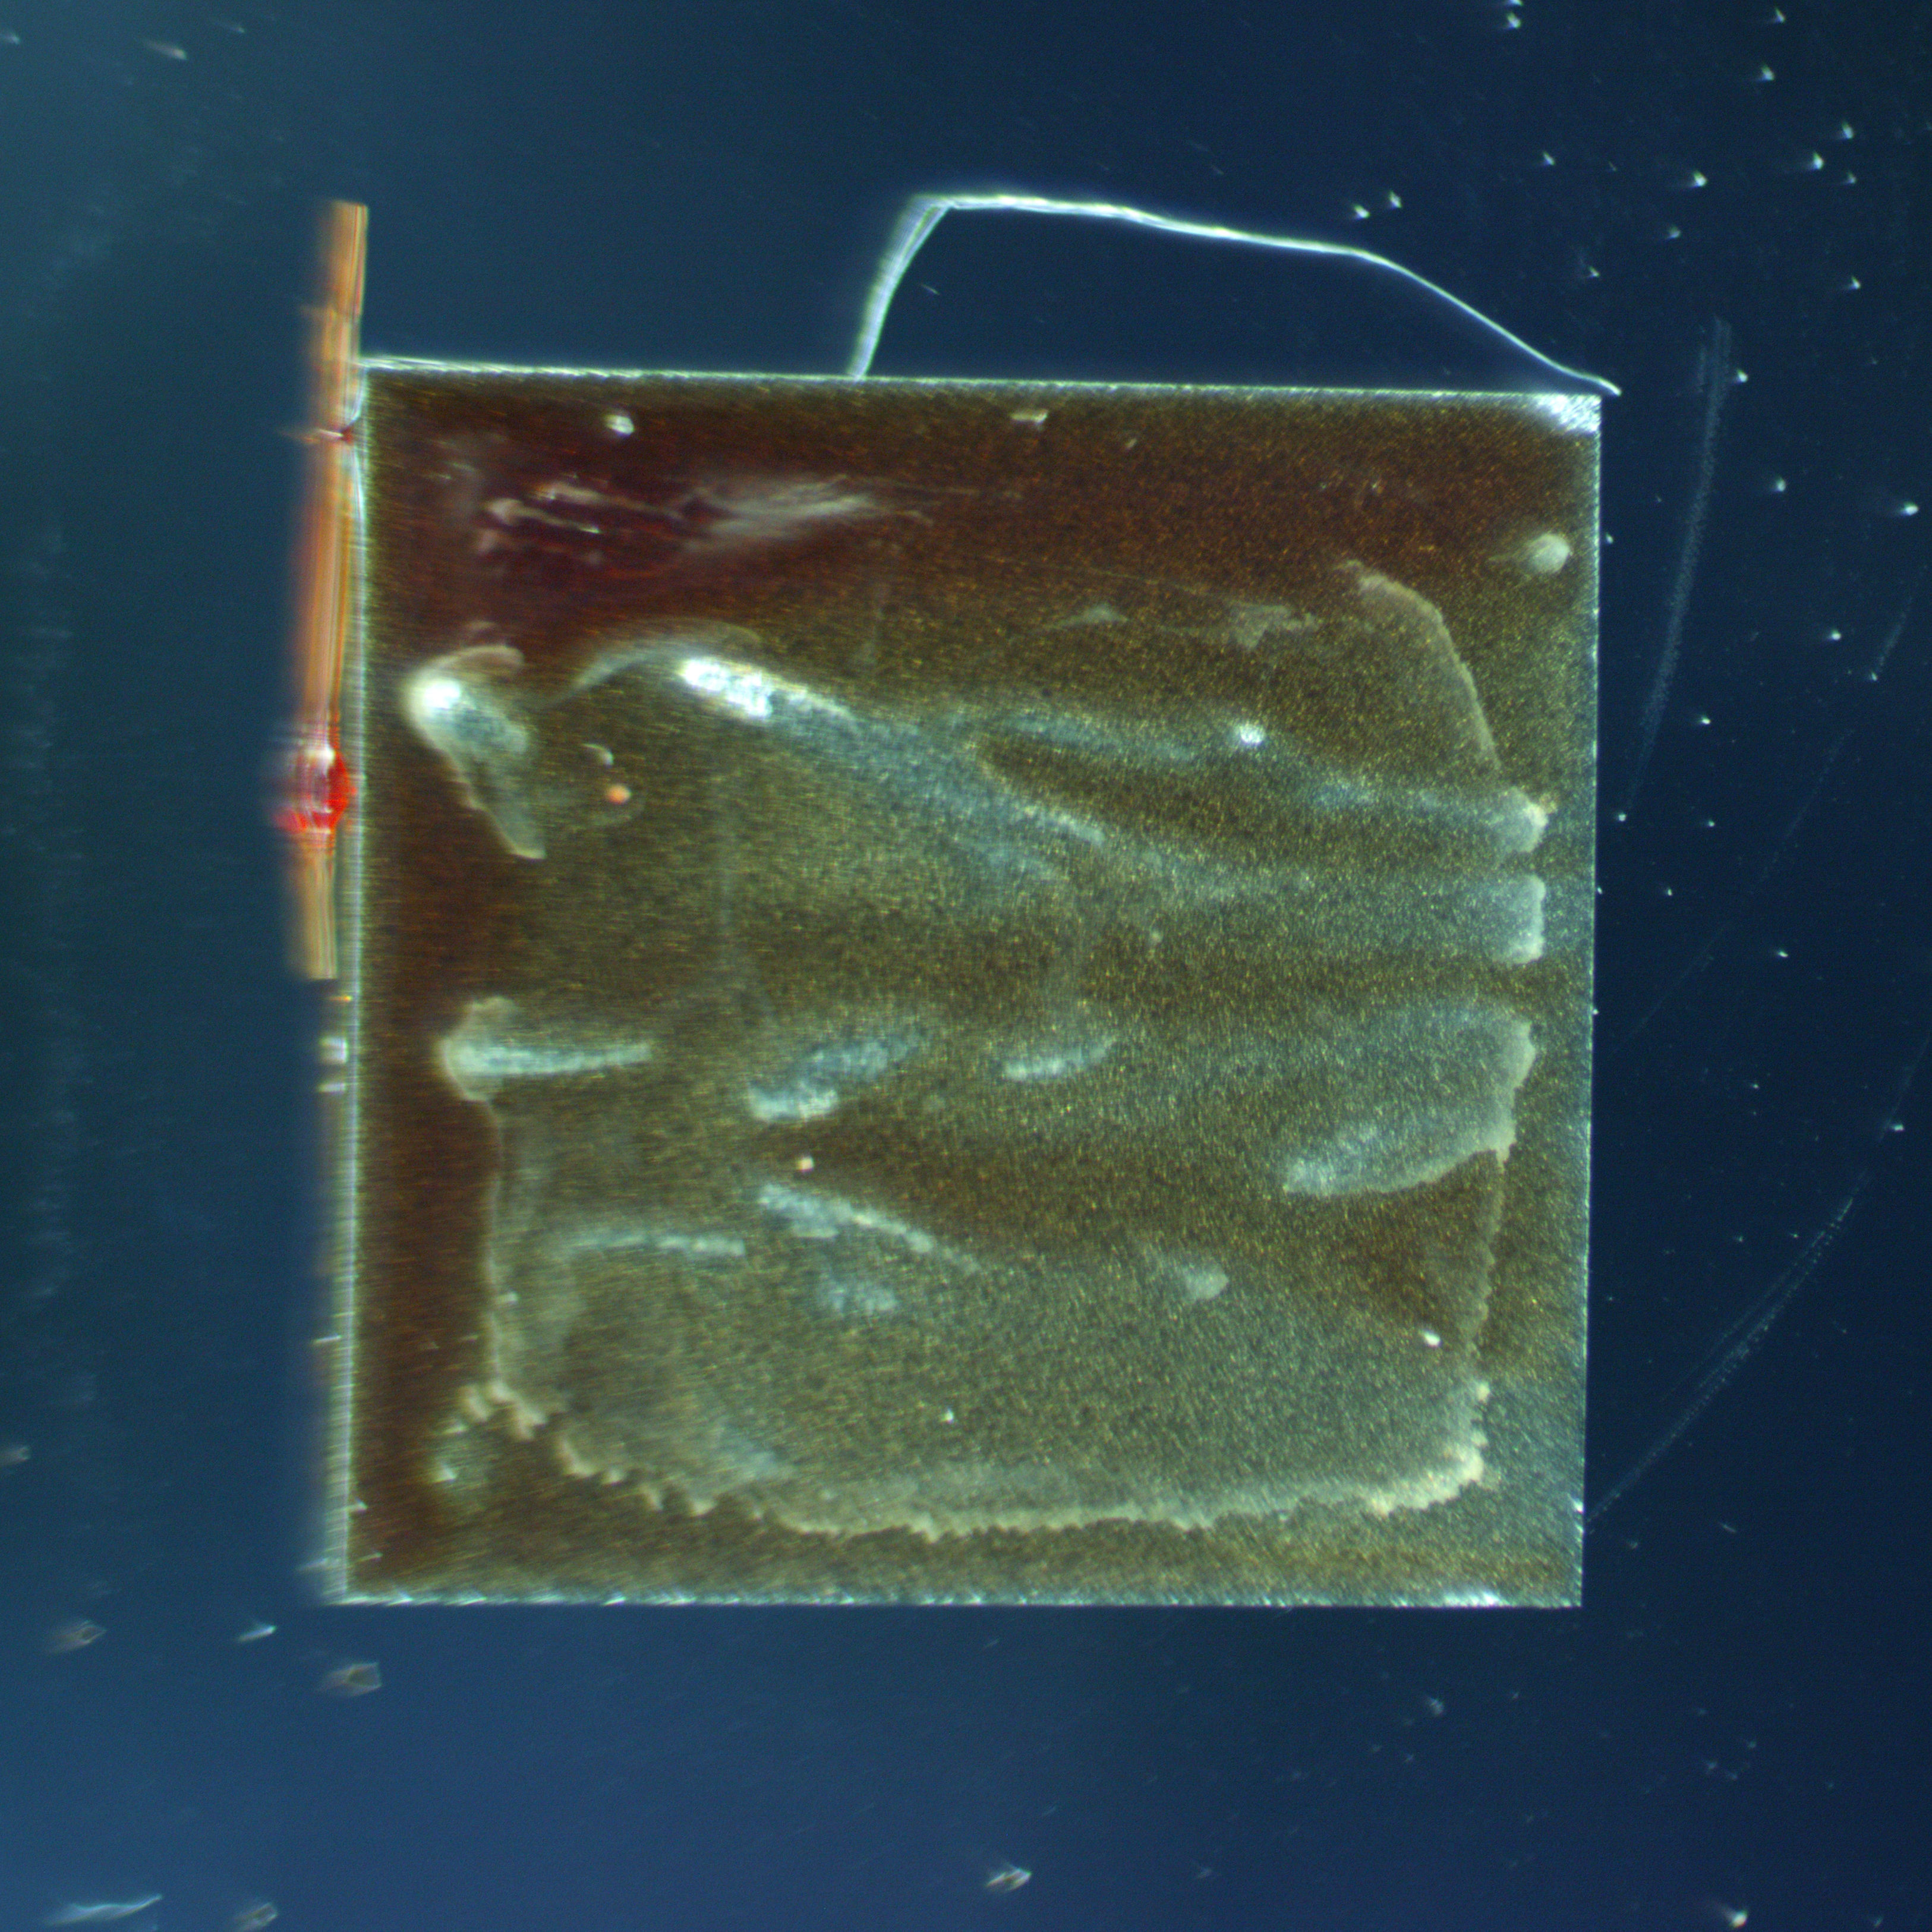
\includegraphics[width=\linewidth]{pics/spincoat/no9/9101.jpg}
        \caption{\textcolor{blue!60!black}{\textbf{Heater 1}}}
    \end{subfigure}
    \hfill
    \begin{subfigure}[t]{0.3\textwidth}
        \centering
        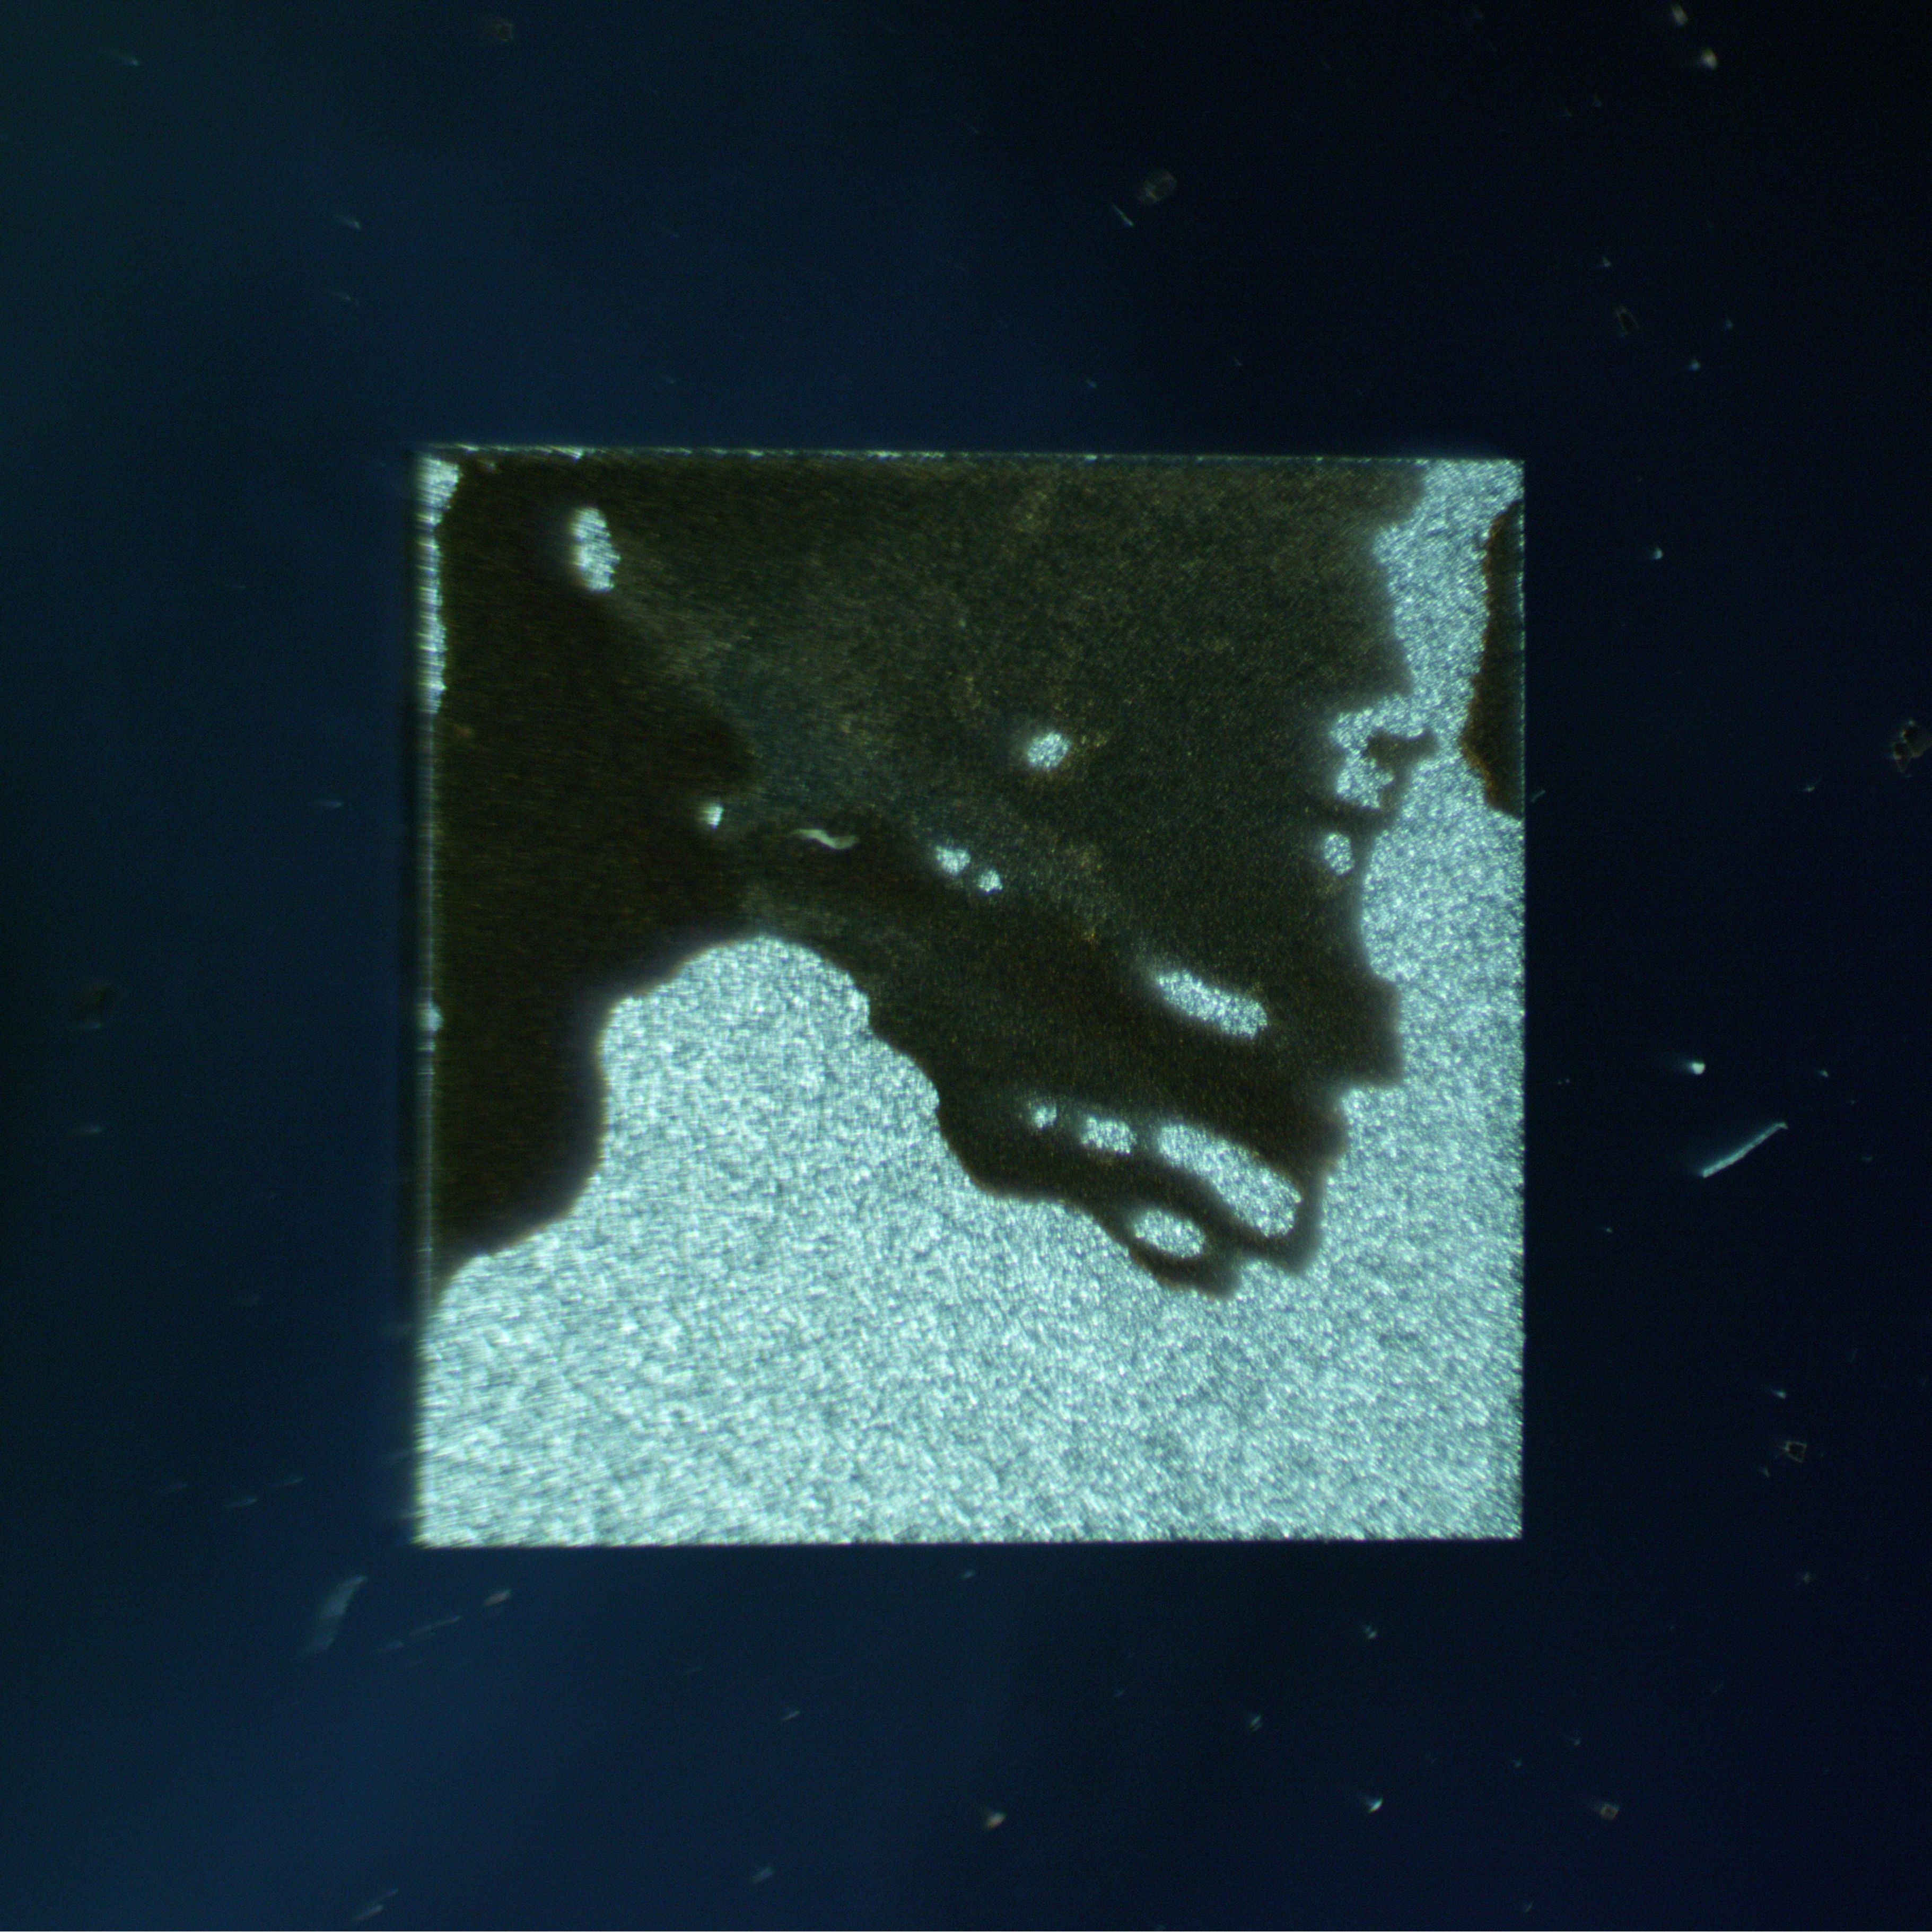
\includegraphics[width=\linewidth]{pics/spincoat/no9/9102.jpg}
        \caption{\textcolor{blue!60!black}{\textbf{Heater 2}}}
    \end{subfigure}
    \hfill
    \begin{subfigure}[t]{0.3\textwidth}
        \centering
        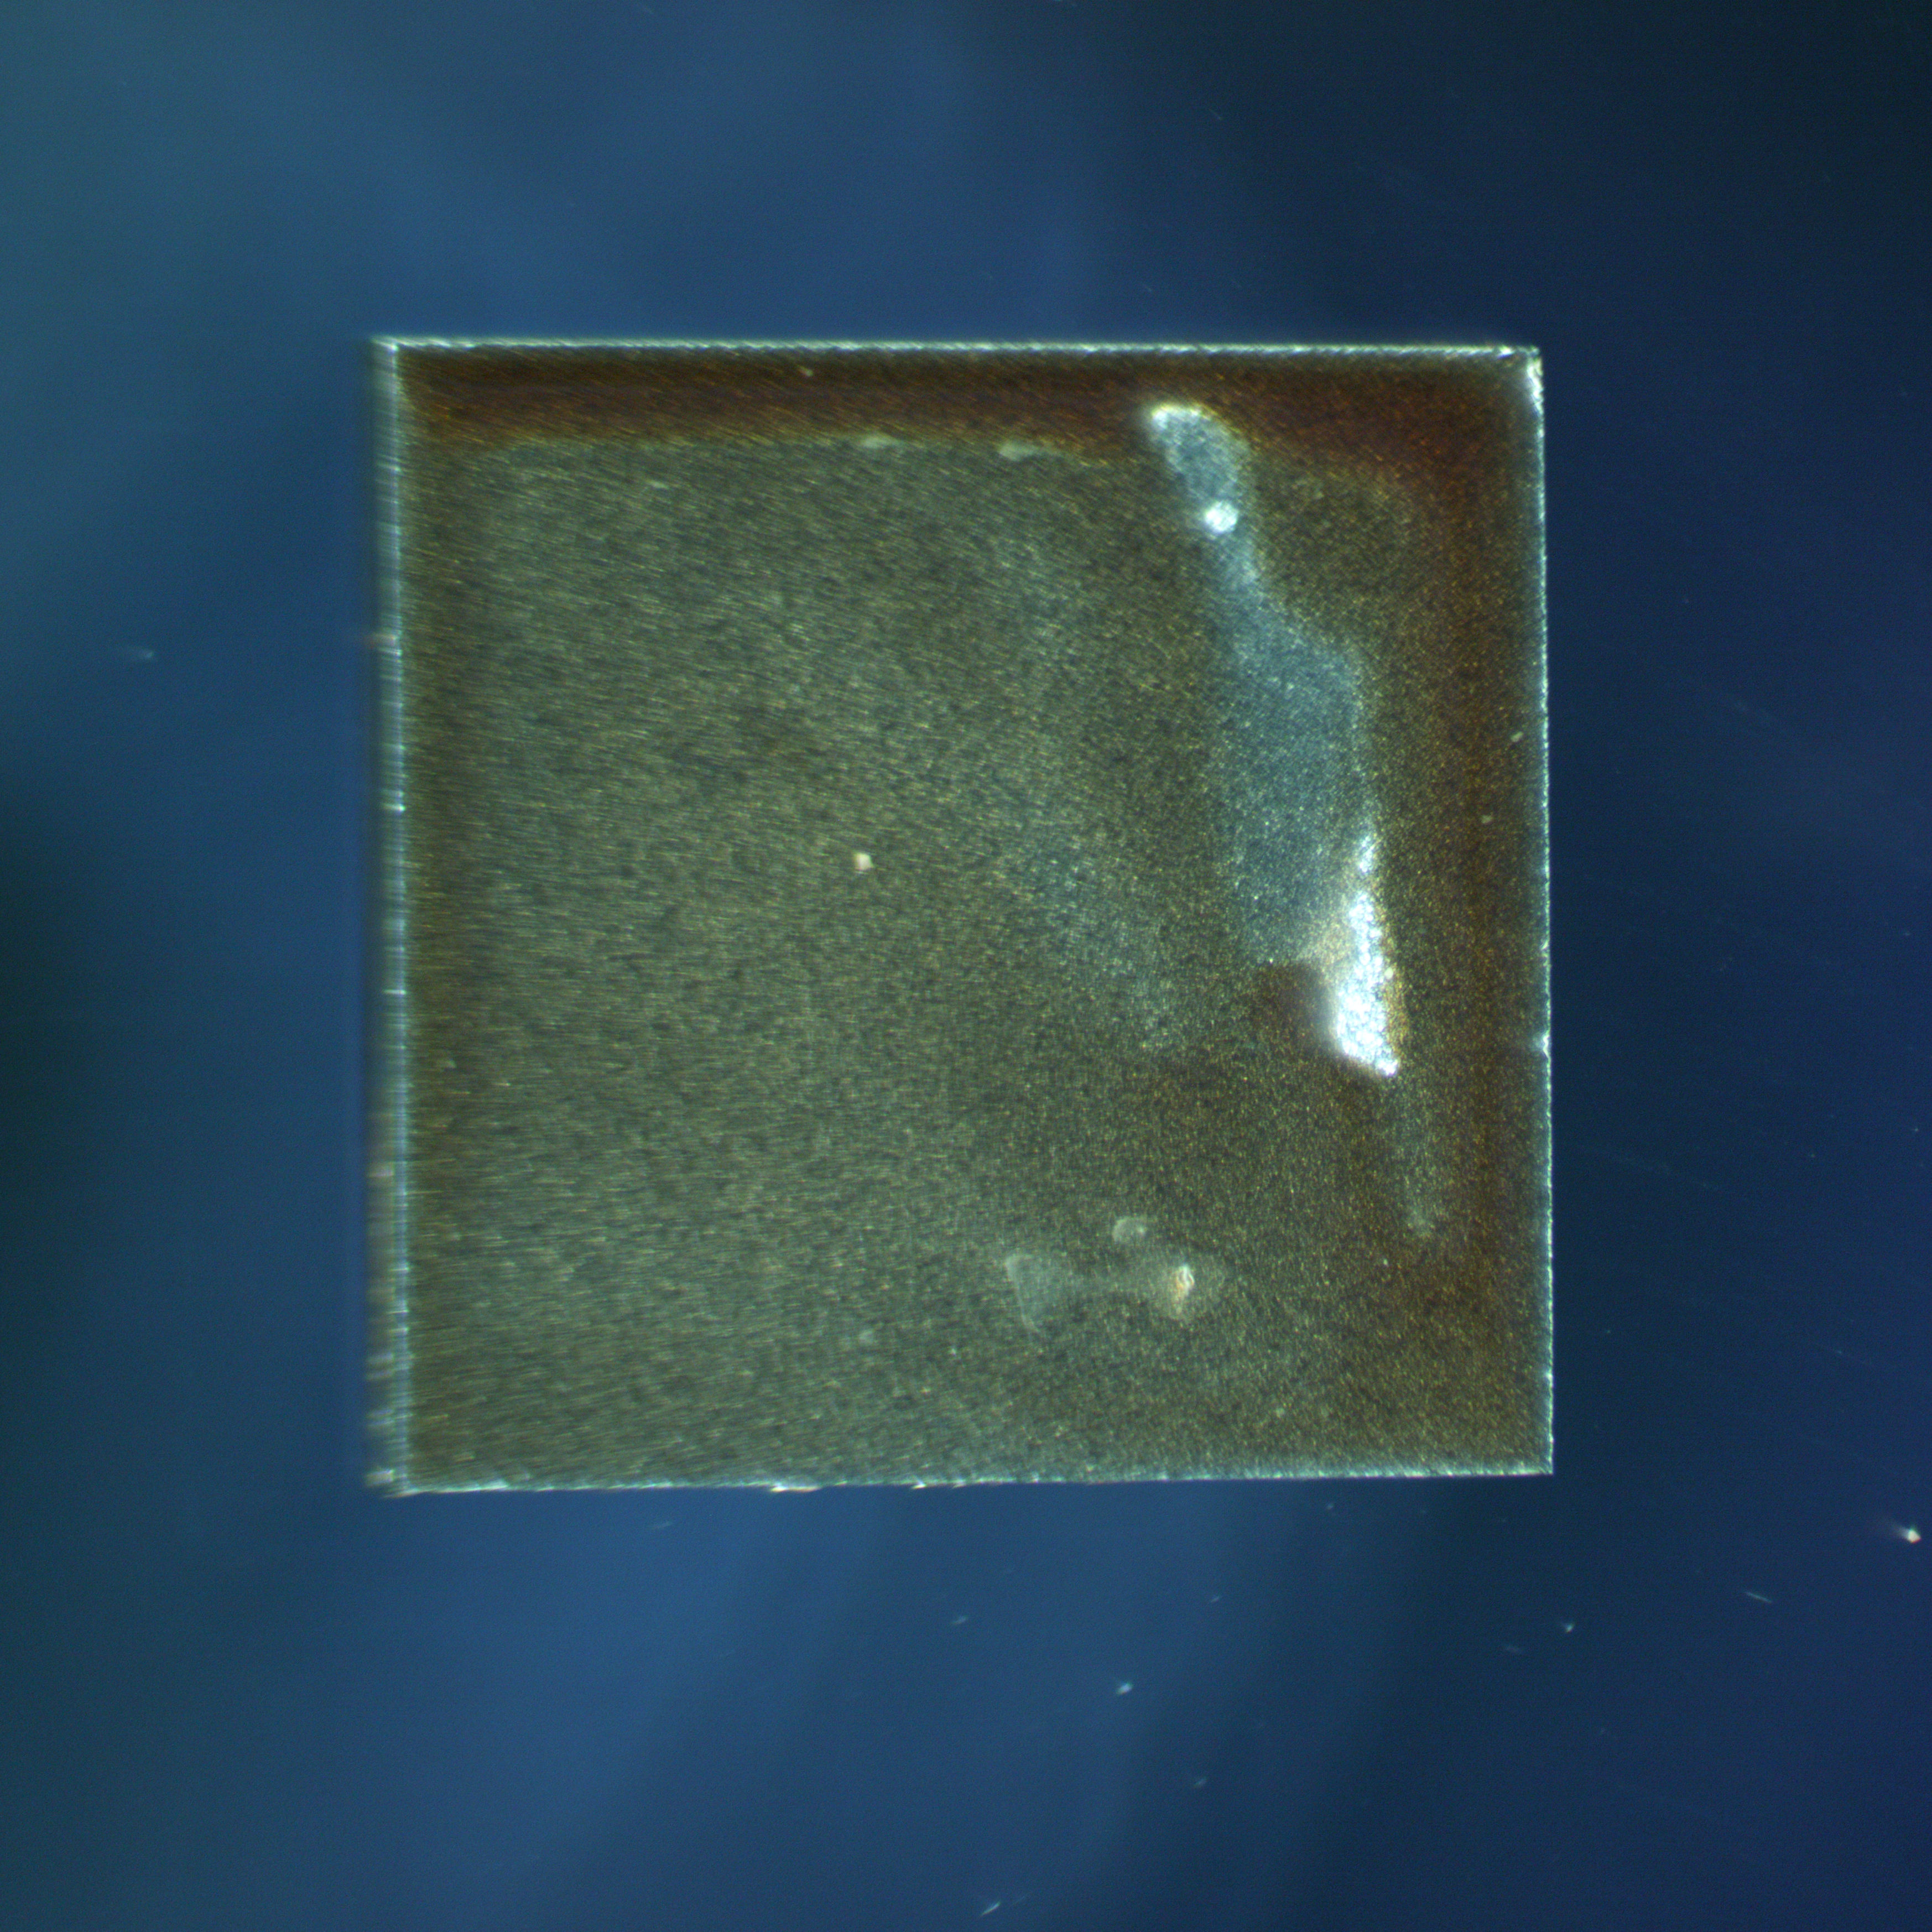
\includegraphics[width=\linewidth]{pics/spincoat/no9/9103.jpg}
        \caption{\textcolor{blue!60!black}{\textbf{Heater 3}}}
    \end{subfigure}

    \vspace{0.8cm}

    % ---------- Row 2 ----------
    \begin{subfigure}[t]{0.3\textwidth}
        \centering
        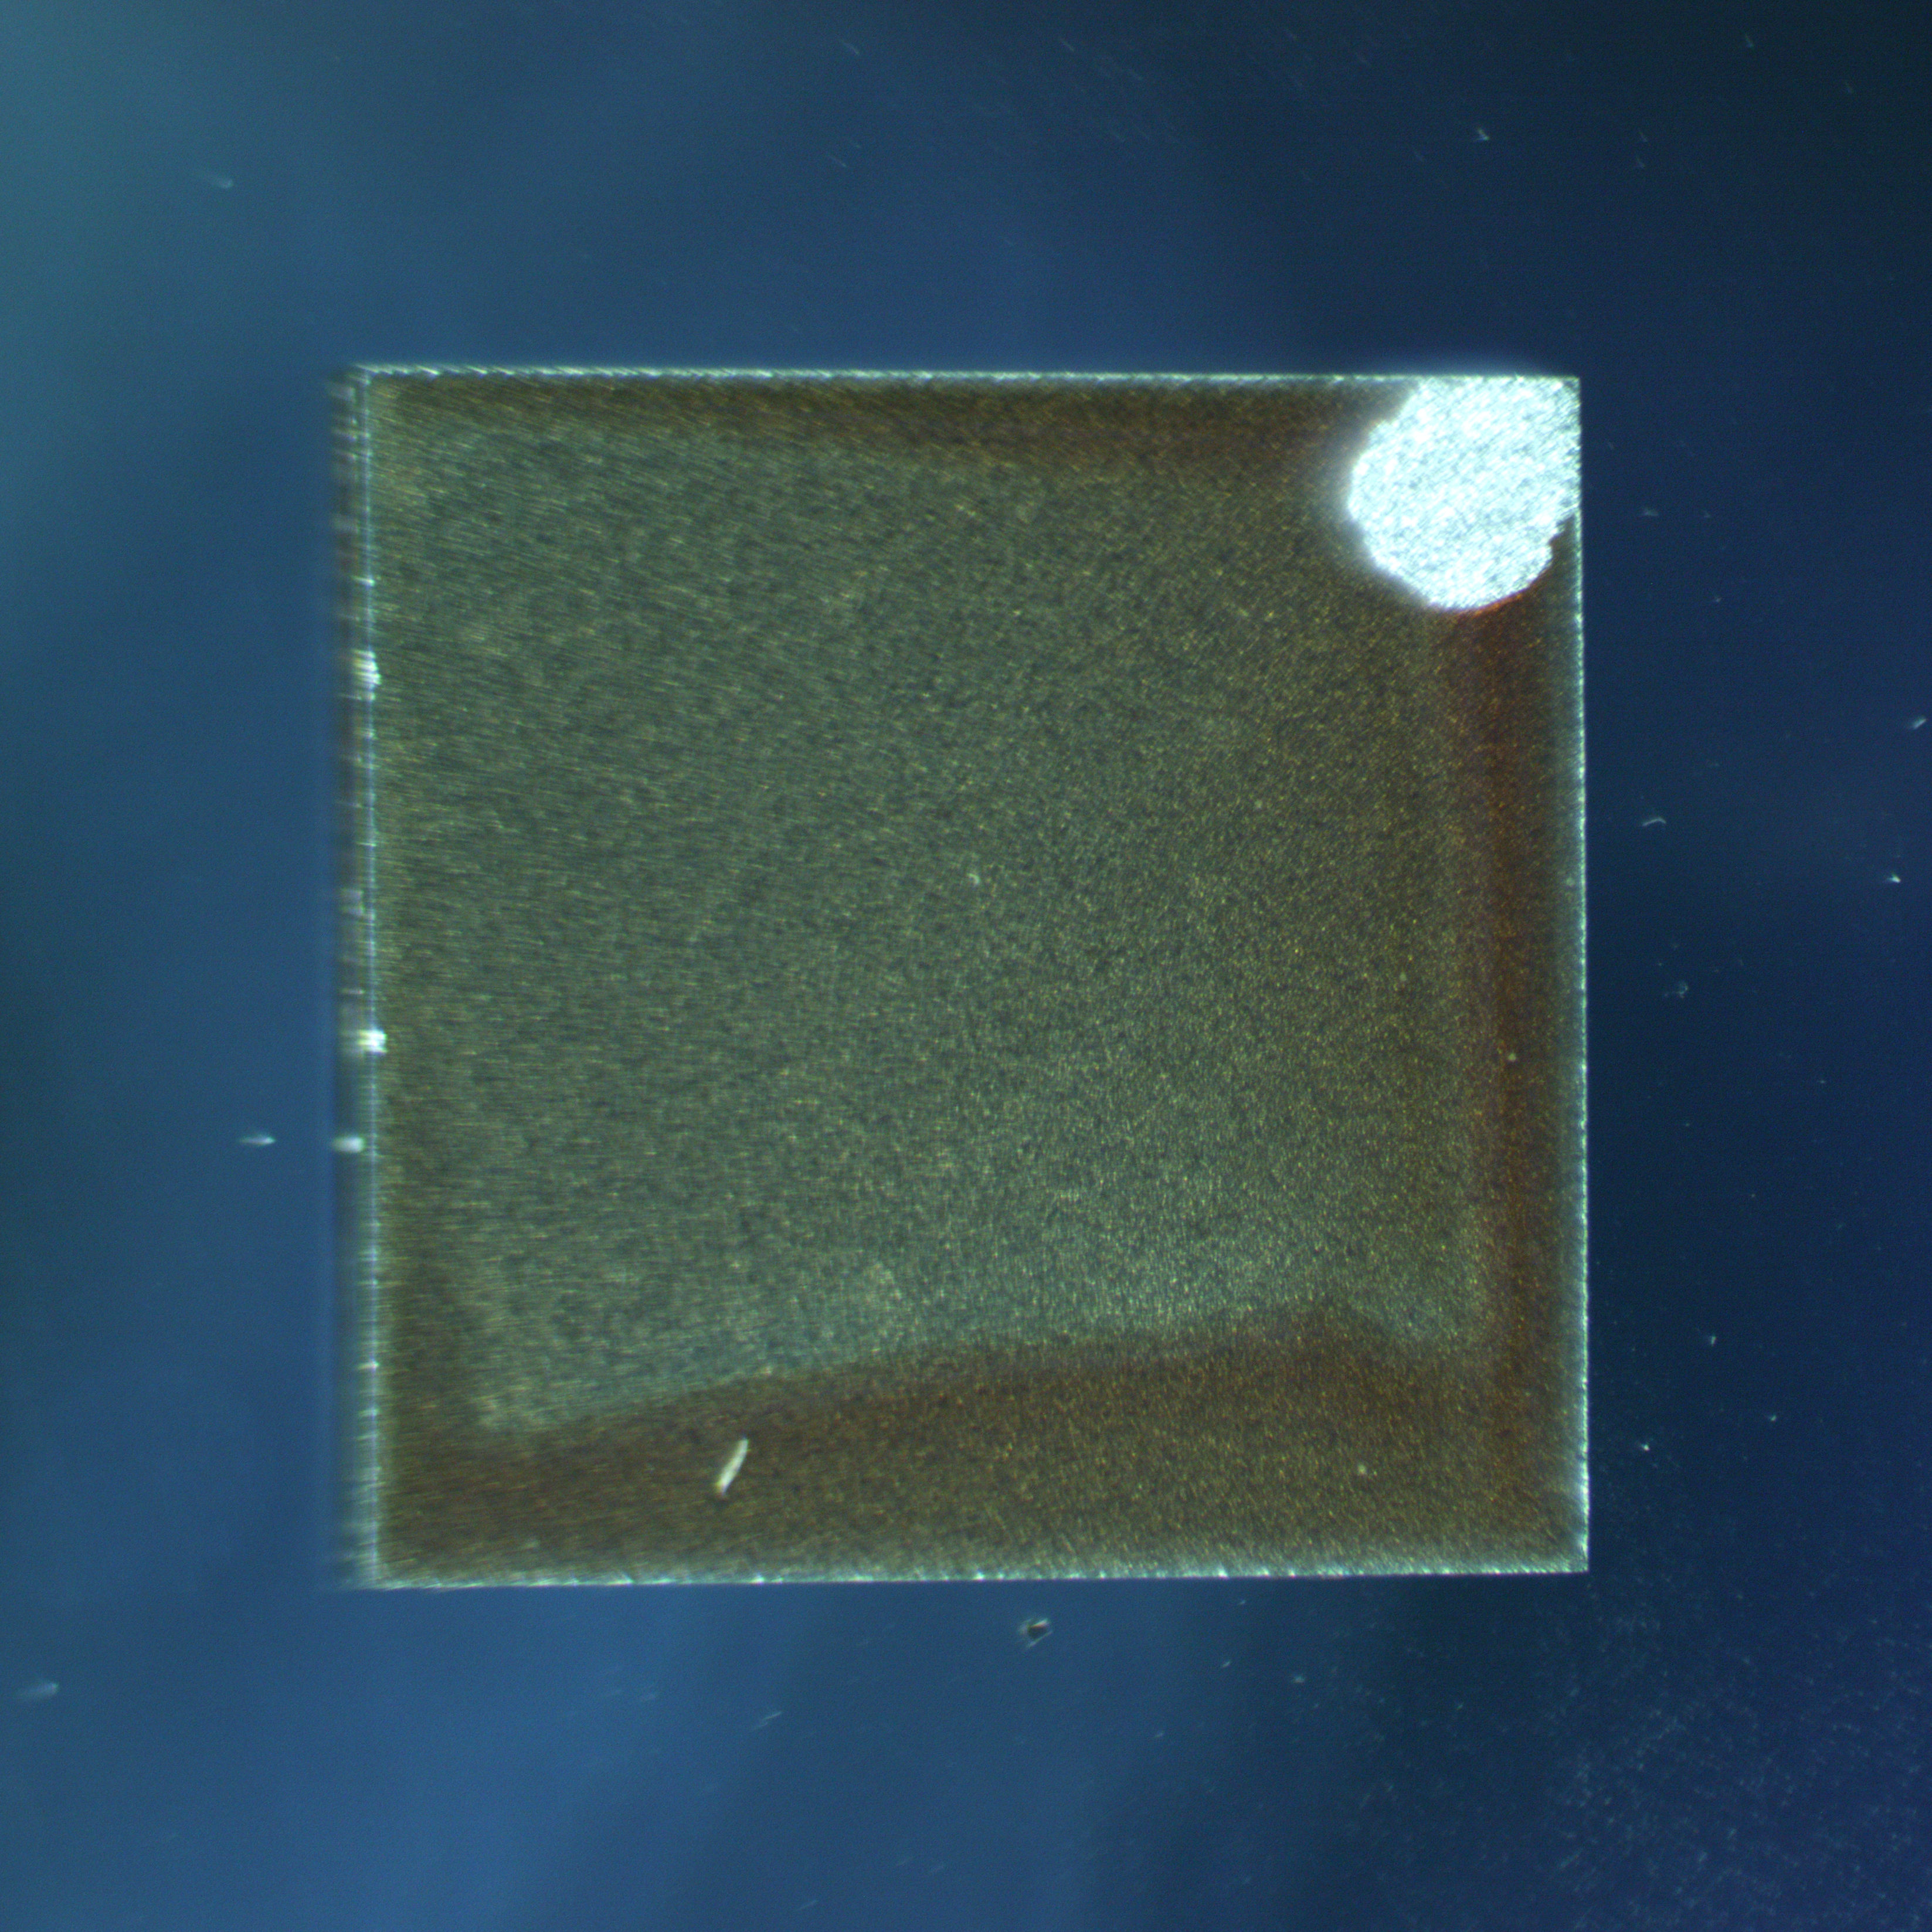
\includegraphics[width=\linewidth]{pics/spincoat/no9/9104.jpg}
        \caption{\textcolor{blue!60!black}{\textbf{Heater 4}}}
    \end{subfigure}
    \hfill
    \begin{subfigure}[t]{0.3\textwidth}
        \centering
        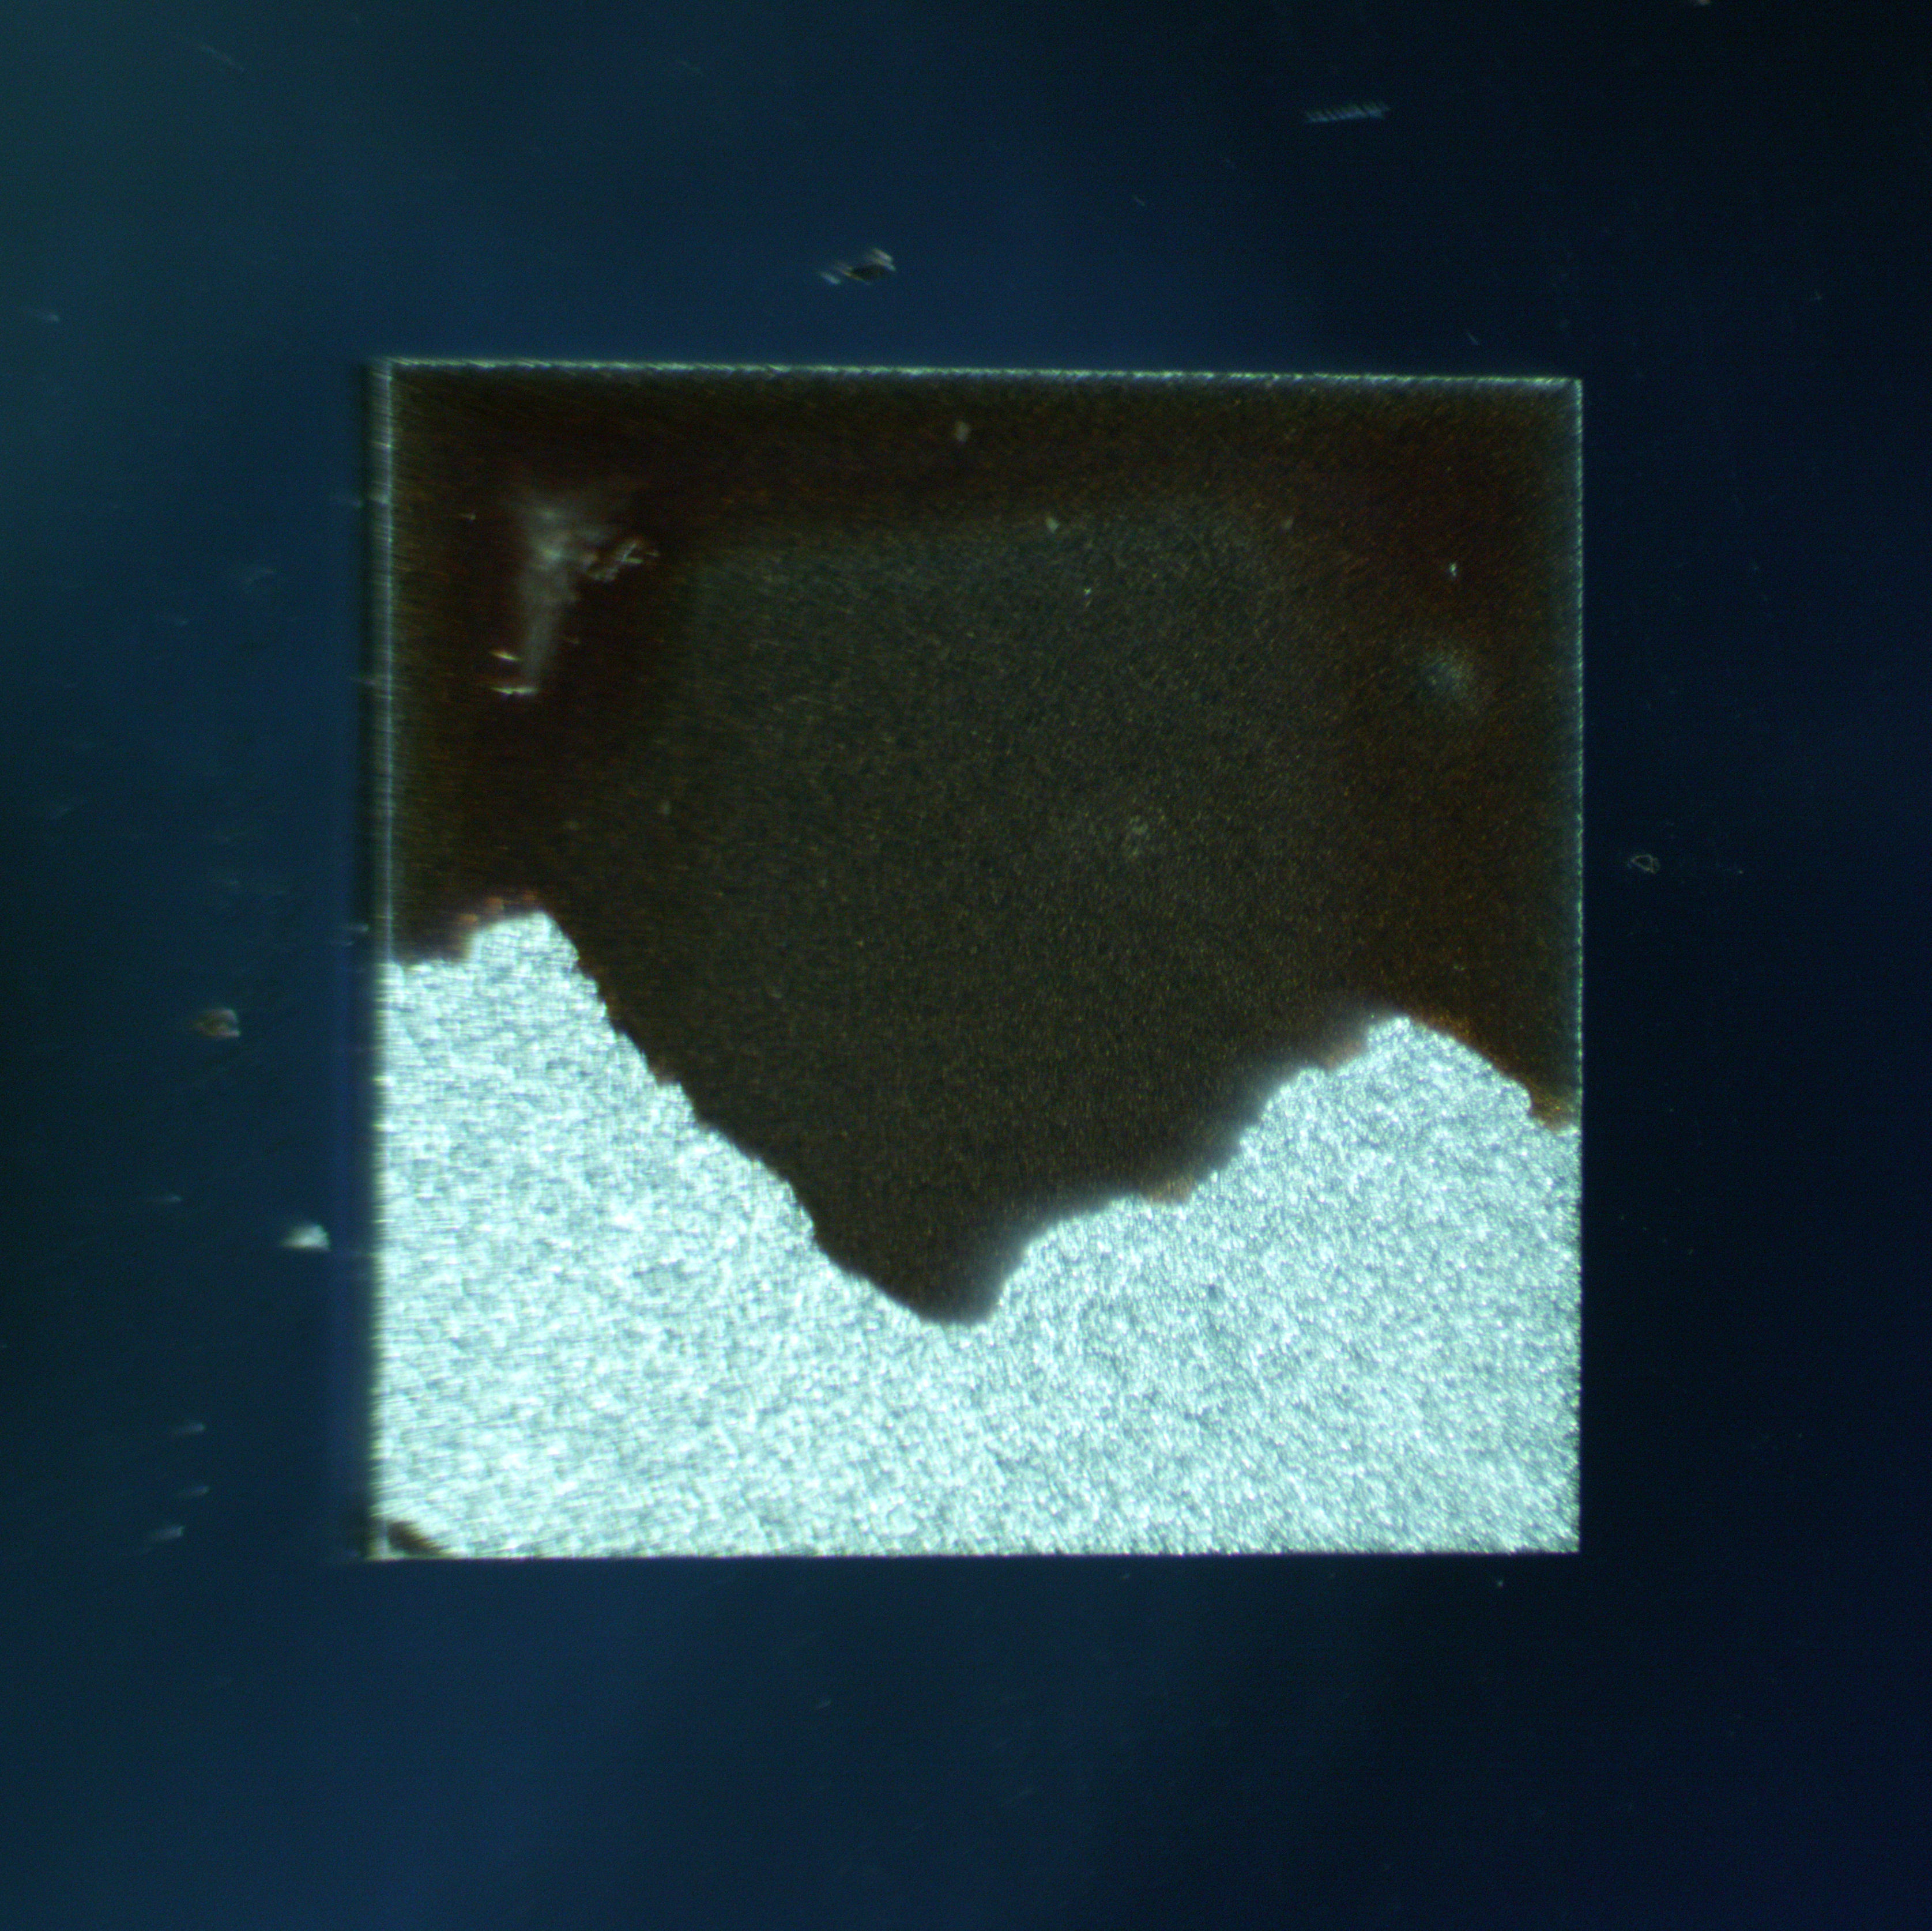
\includegraphics[width=\linewidth]{pics/spincoat/no9/9105.jpg}
        \caption{\textcolor{blue!60!black}{\textbf{Heater 5*}}}
    \end{subfigure}
    \hfill
    \begin{subfigure}[t]{0.3\textwidth}
        \centering
        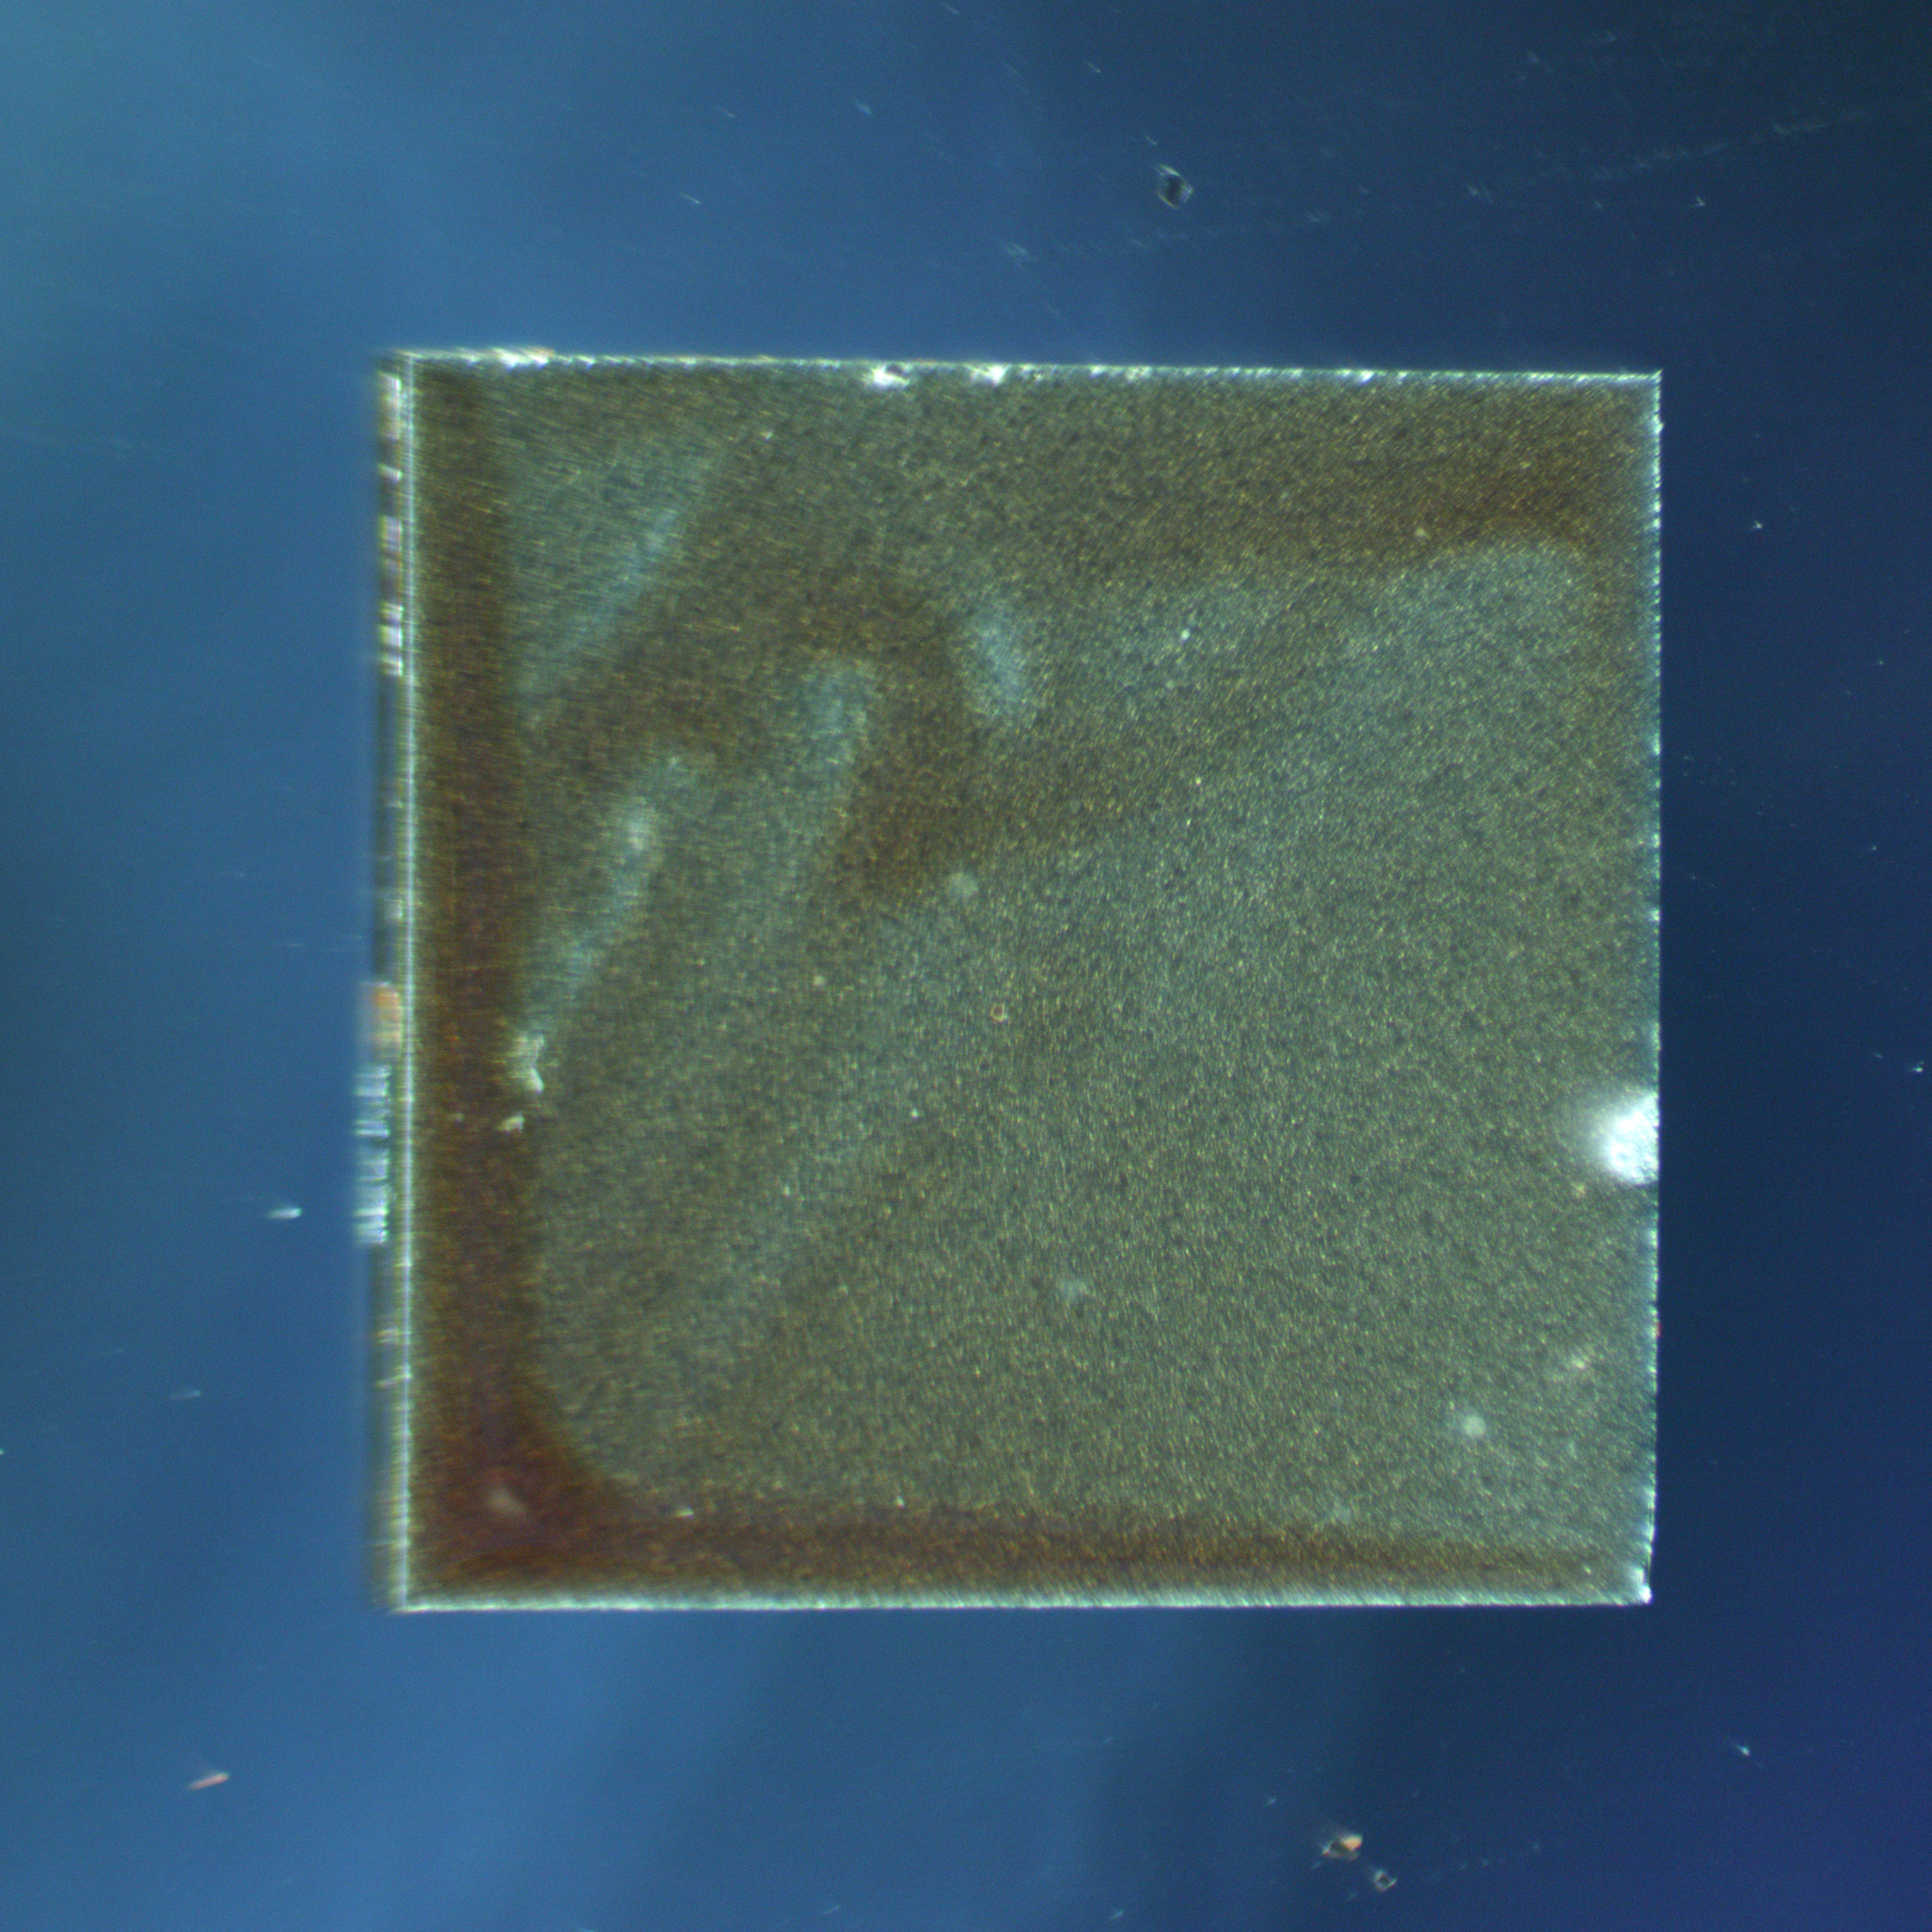
\includegraphics[width=\linewidth]{pics/spincoat/no9/9106.jpg}
        \caption{\textcolor{blue!60!black}{\textbf{Heater 6}}}
    \end{subfigure}

    \vspace{0.8cm}

    % ---------- Row 3 ----------
    \begin{subfigure}[t]{0.3\textwidth}
        \centering
        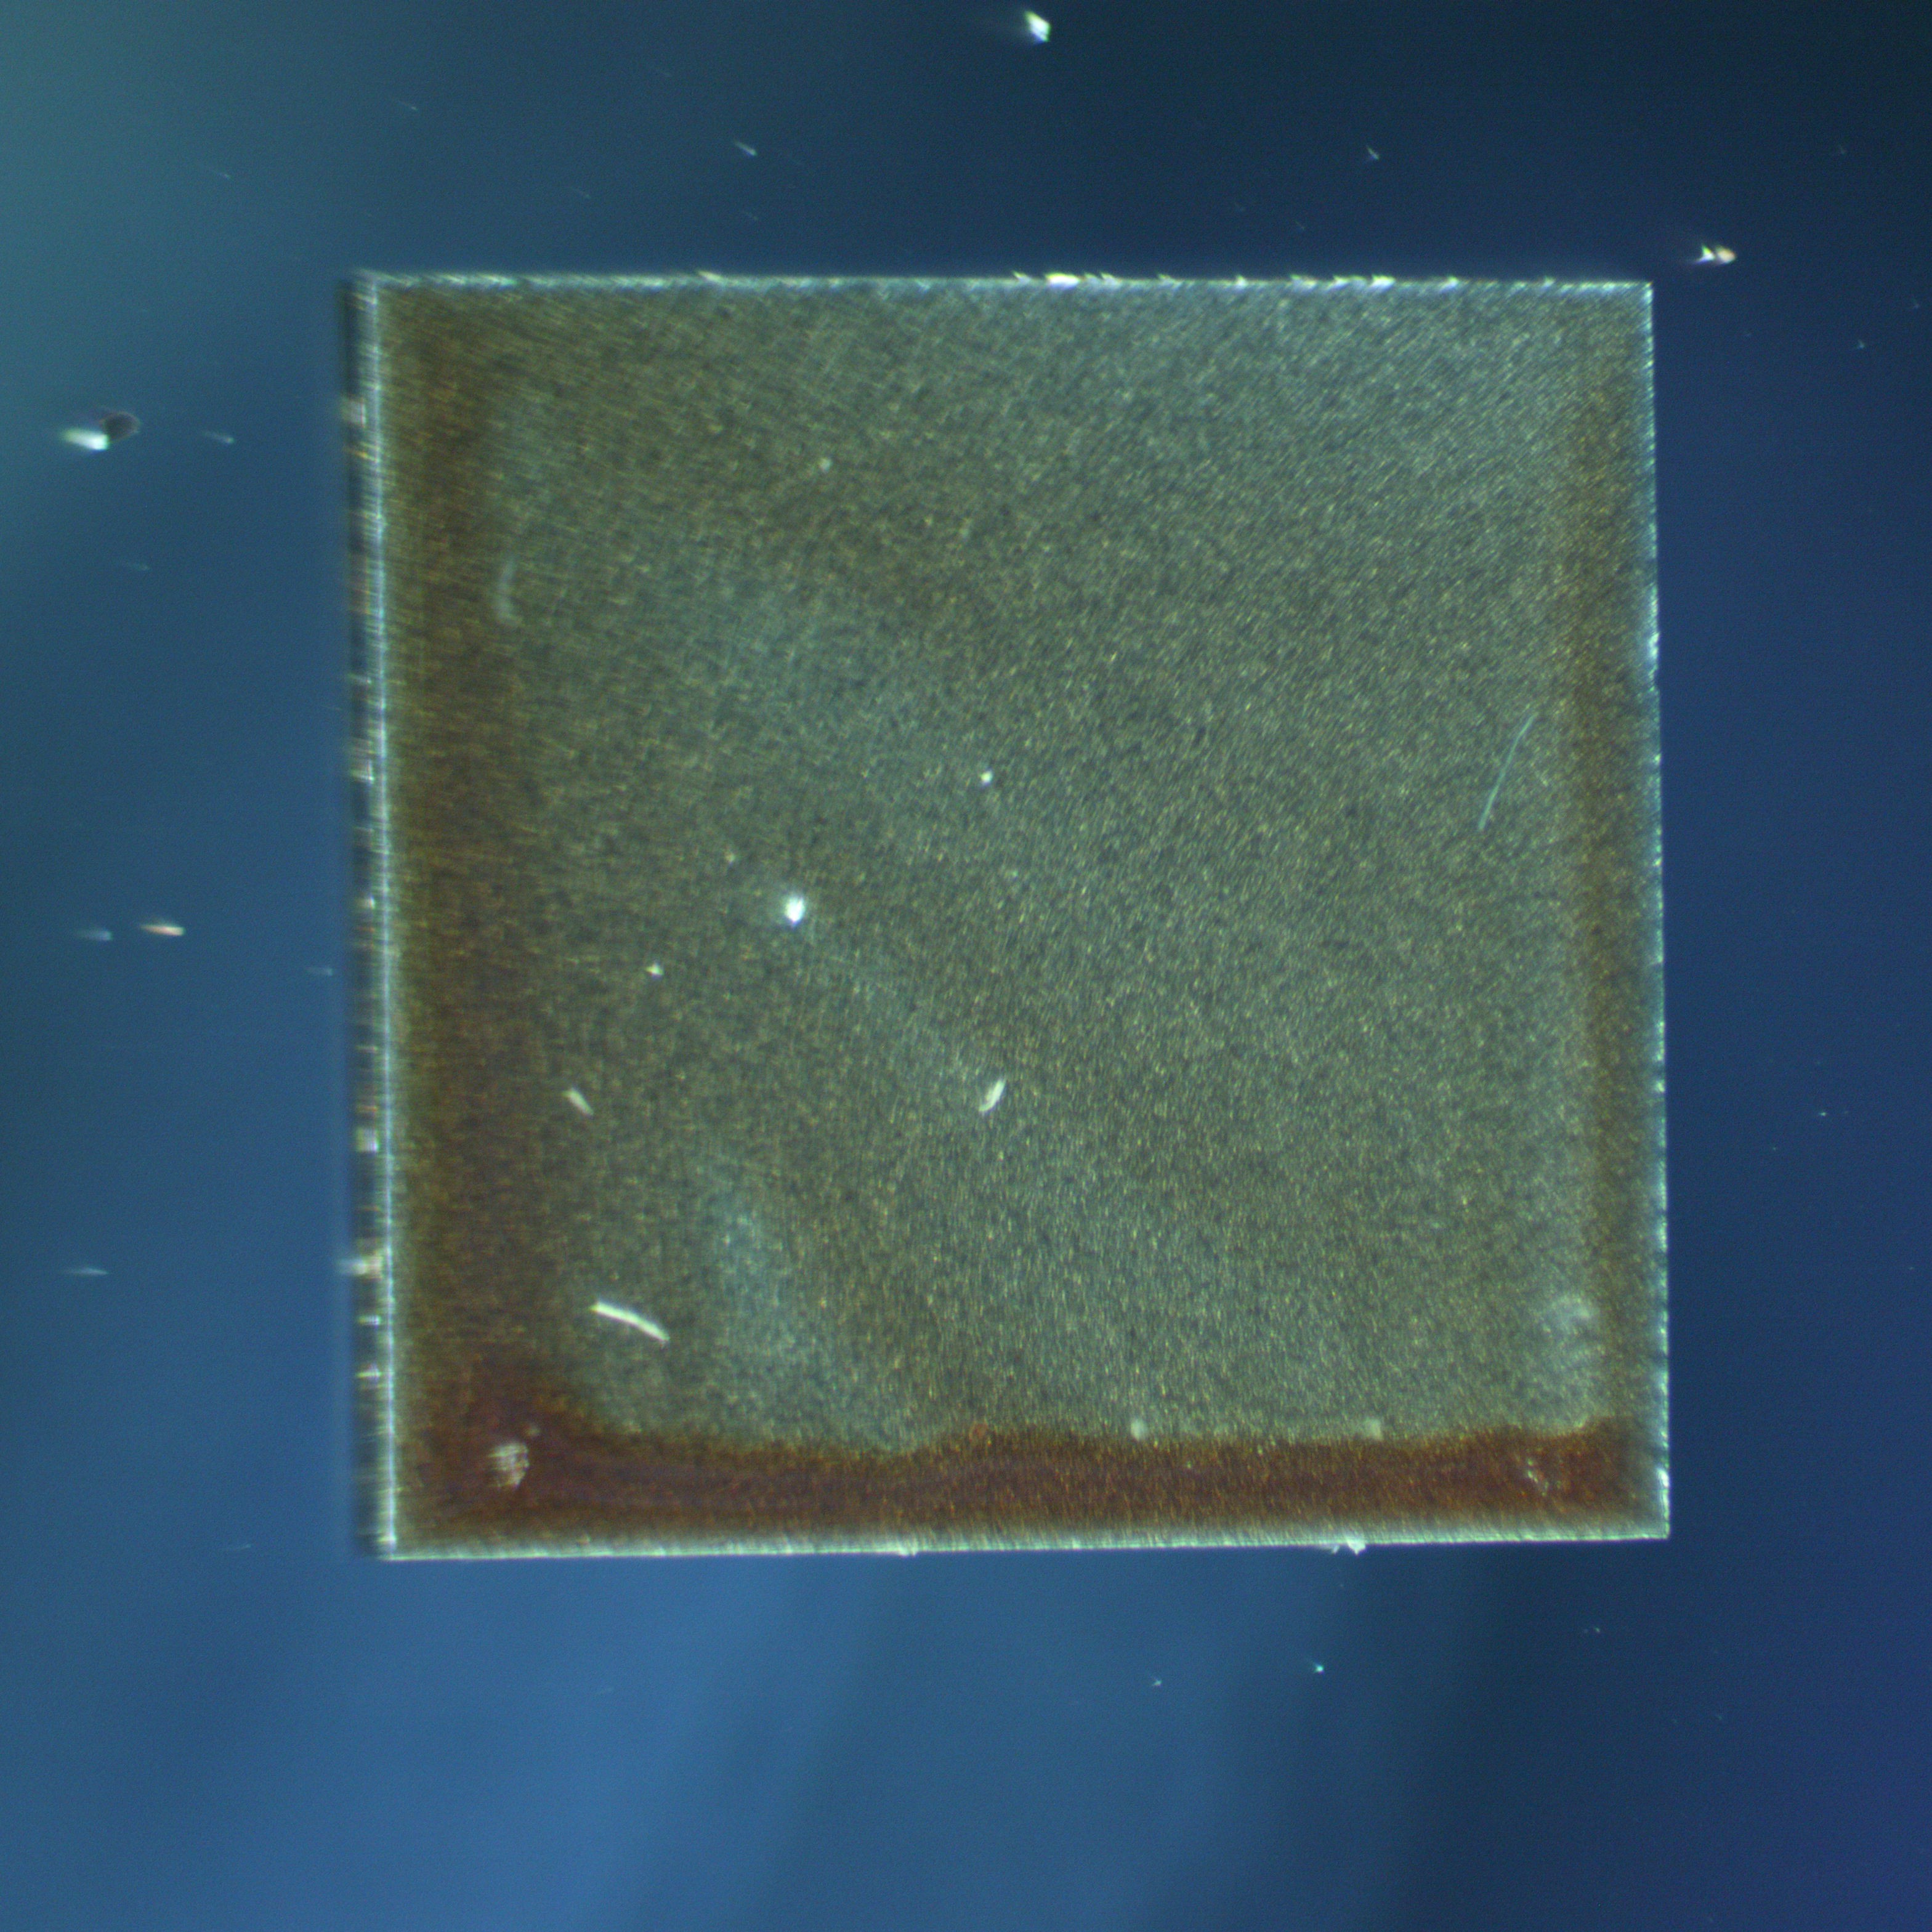
\includegraphics[width=\linewidth]{pics/spincoat/no9/9107.jpg}
        \caption{\textcolor{blue!60!black}{\textbf{Heater 7}}}
    \end{subfigure}
    \hfill
    \begin{subfigure}[t]{0.3\textwidth}
        \centering
        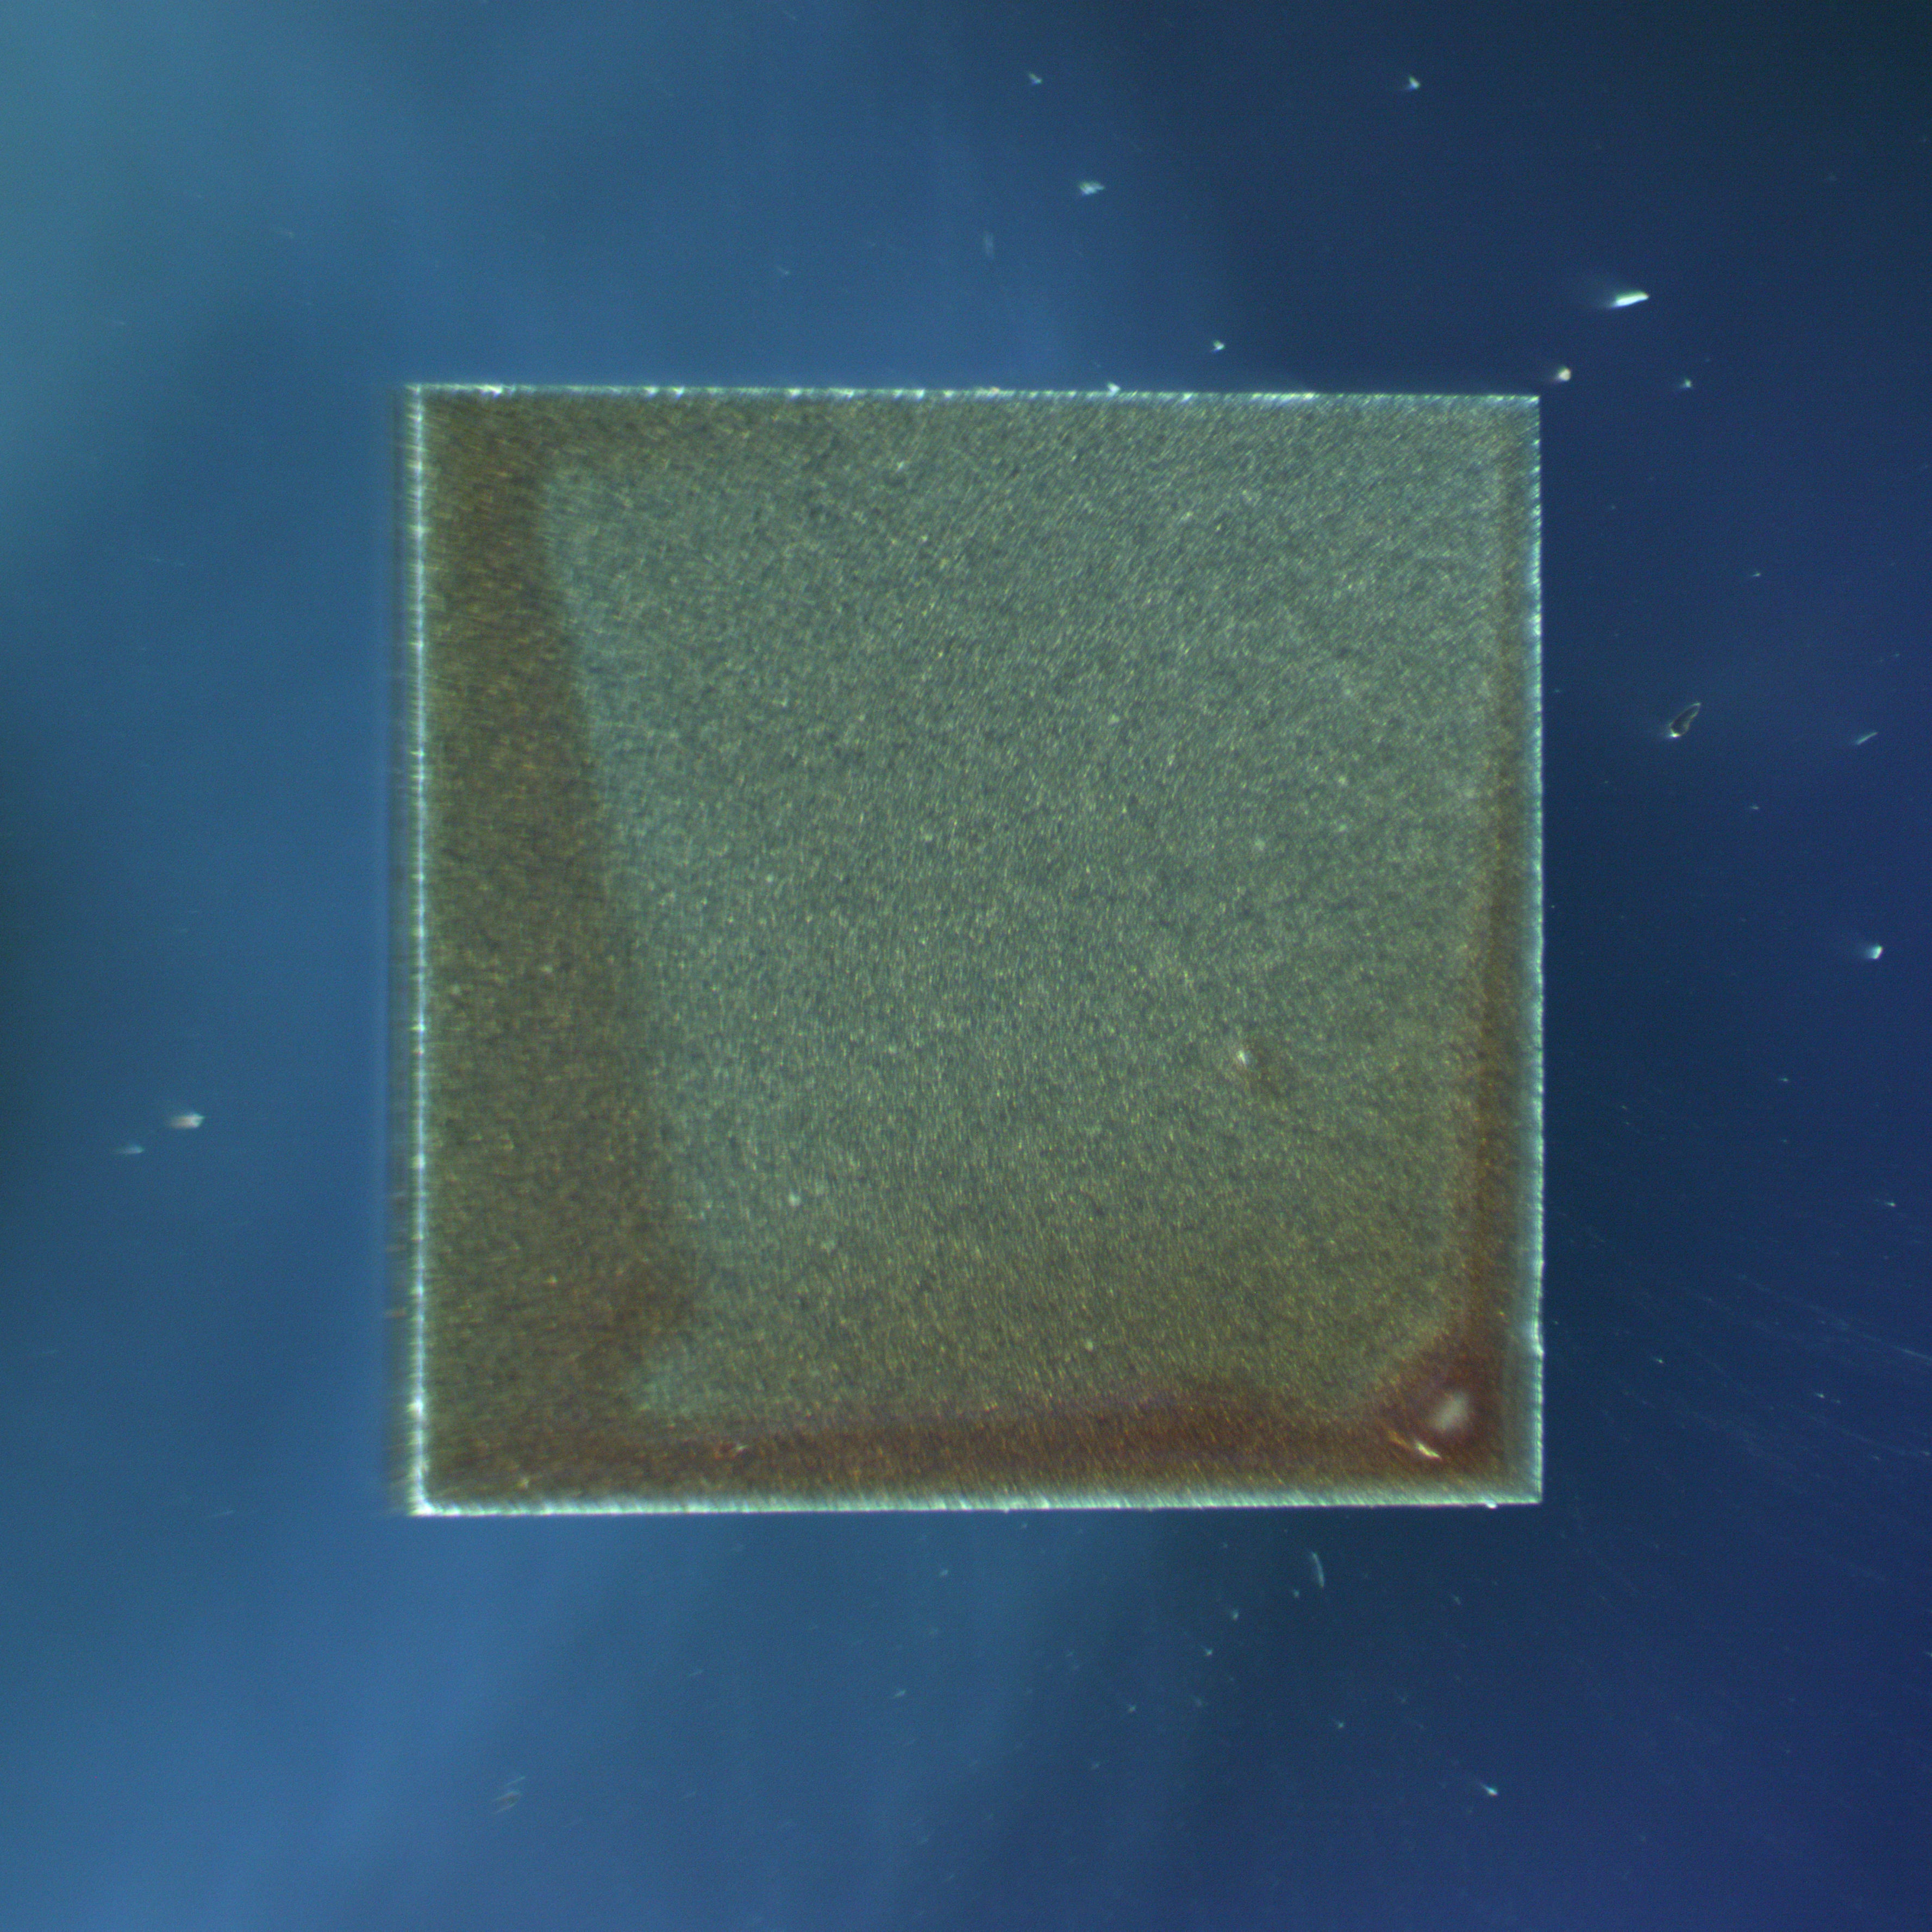
\includegraphics[width=\linewidth]{pics/spincoat/no9/9108.jpg}
        \caption{\textcolor{blue!60!black}{\textbf{Heater 8}}}
    \end{subfigure}
    \hfill
    \begin{subfigure}[t]{0.3\textwidth}
        \centering
        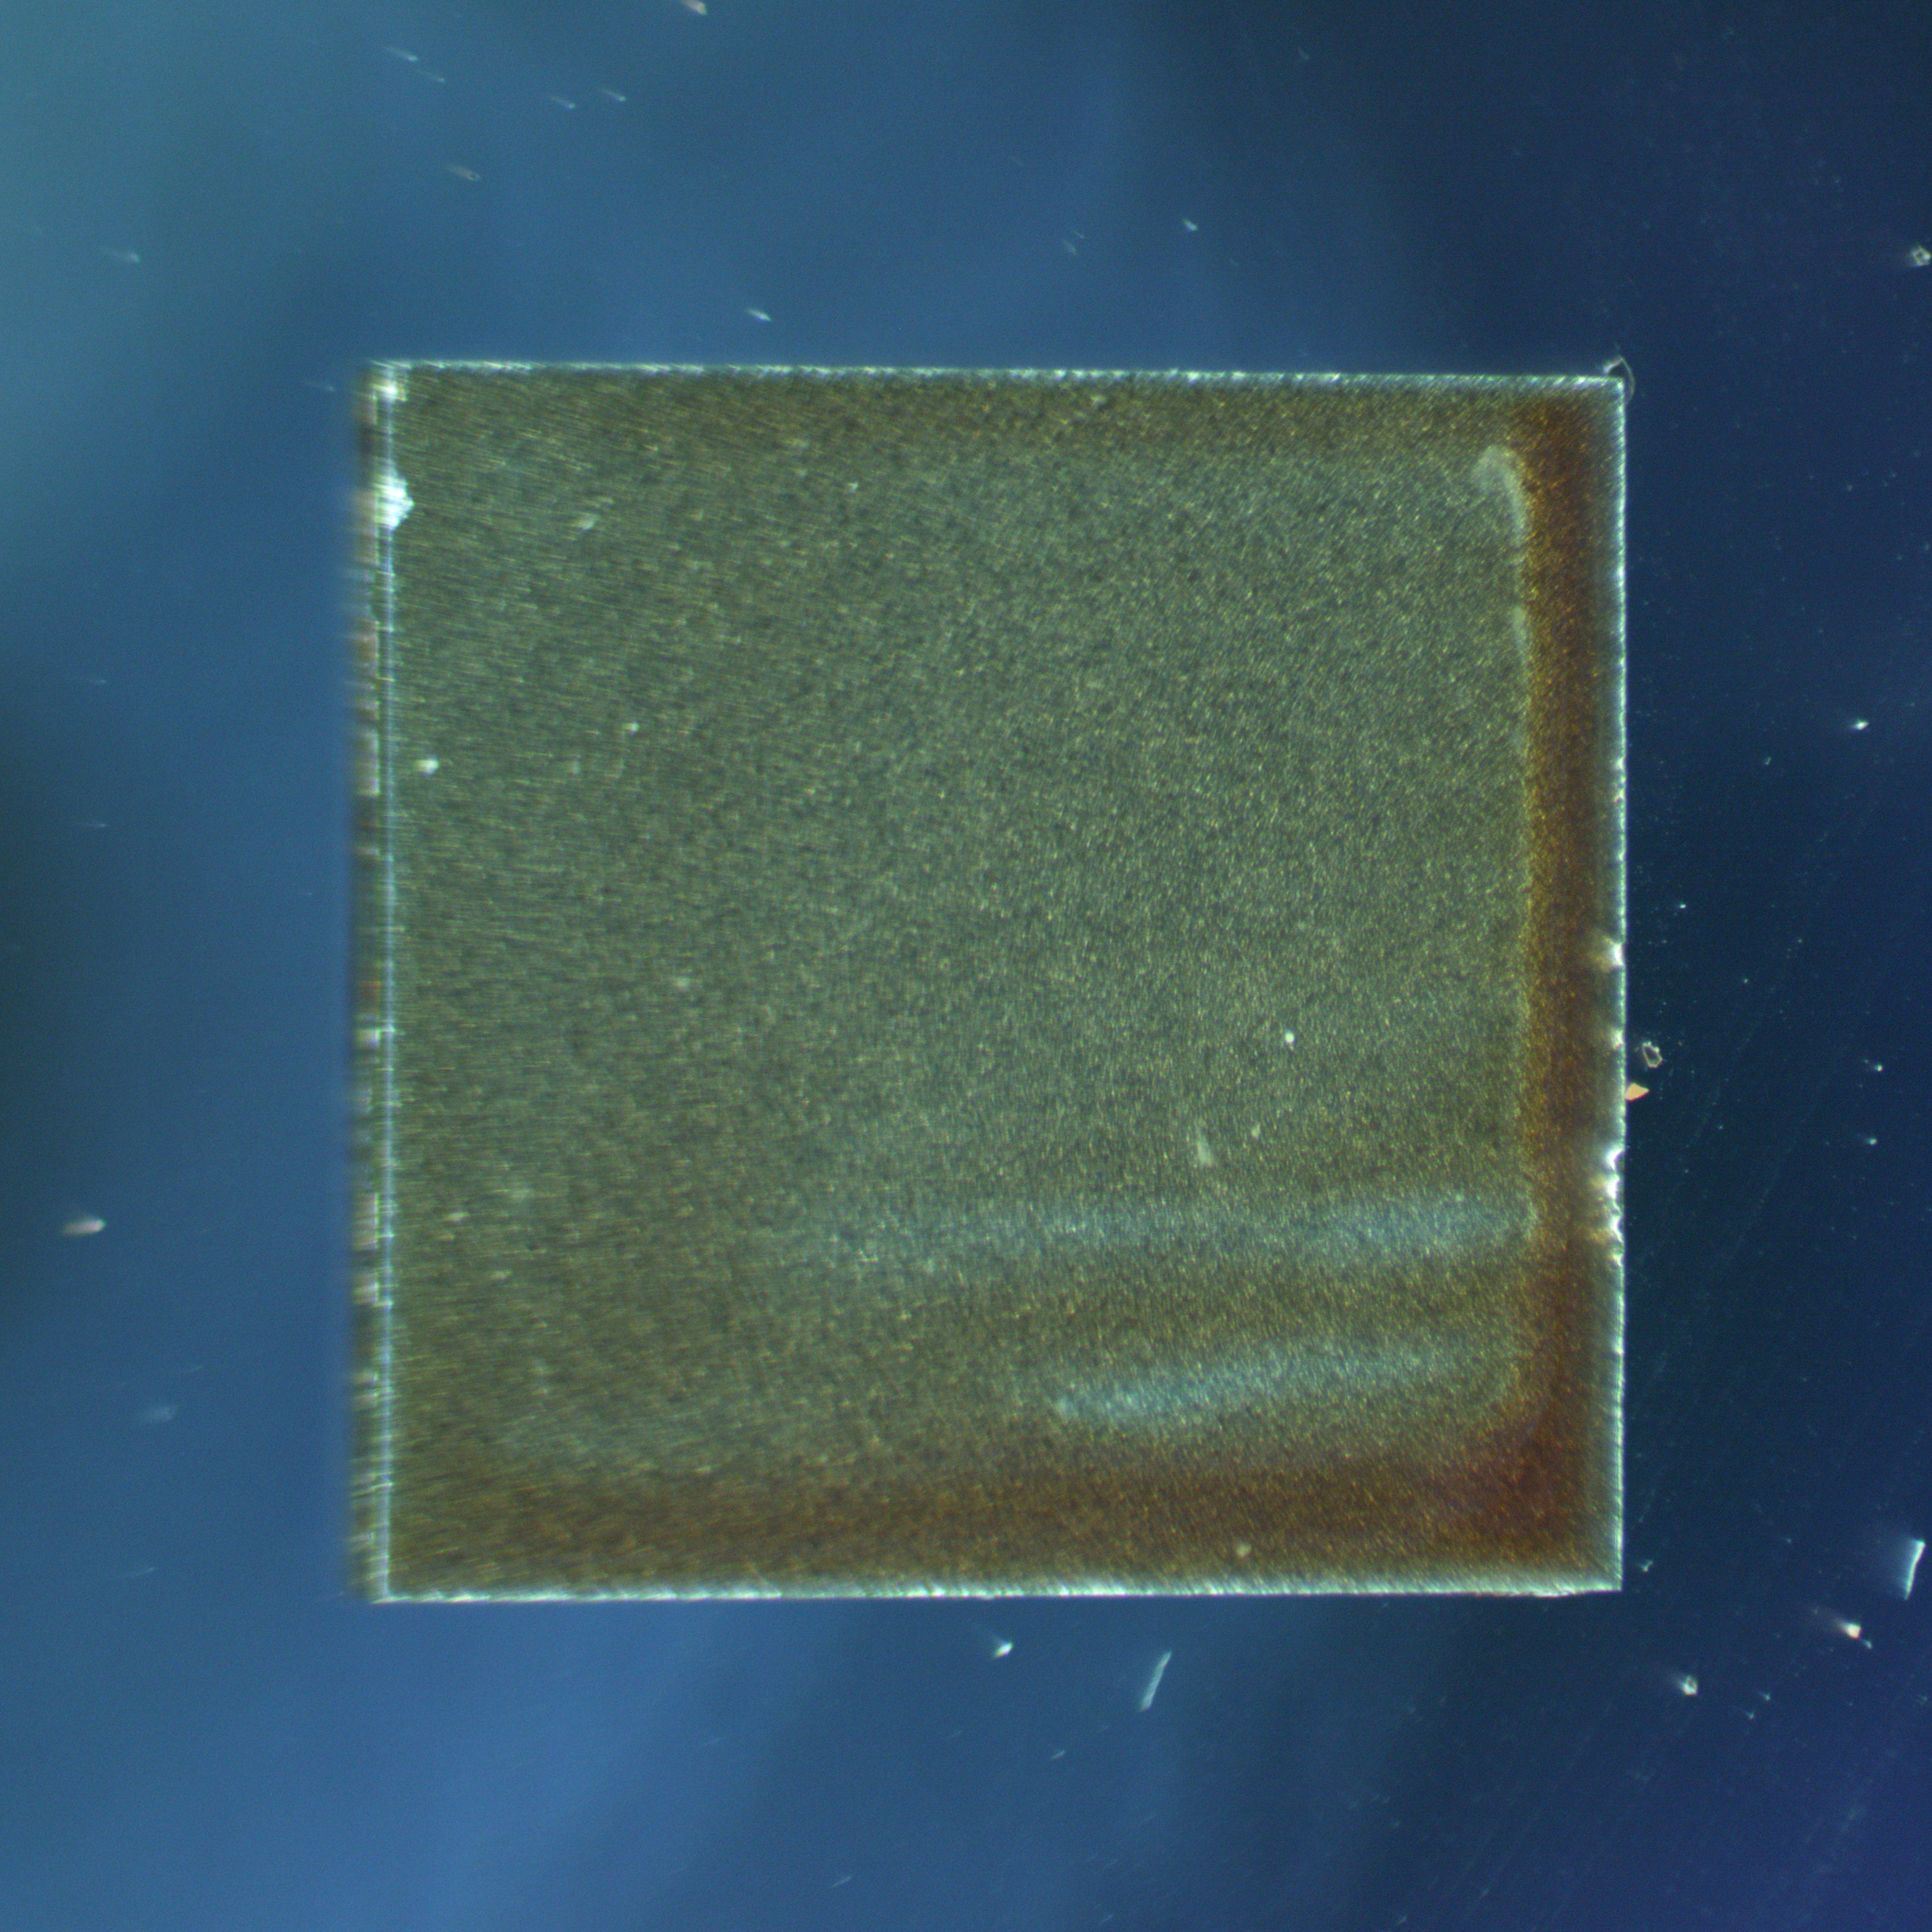
\includegraphics[width=\linewidth]{pics/spincoat/no9/9109.jpg}
        \caption{\textcolor{blue!60!black}{\textbf{Heater 9}}}
    \end{subfigure}

    \caption[Optical Images of the Heater in Passivation Test \#9]{Optical images of the nine Heater of the coating test \#9. The two heaters that could be removed from the glue are highlighted in blue and the height measurement was taken of those marked by a "*"}
    \label{fig:PT9}
\end{figure}
%================================================================================
%================================================================================
\begin{figure}[htbp]
    \centering

    % ---------- Row 1 ----------
    \begin{subfigure}[t]{0.3\textwidth}
        \centering
        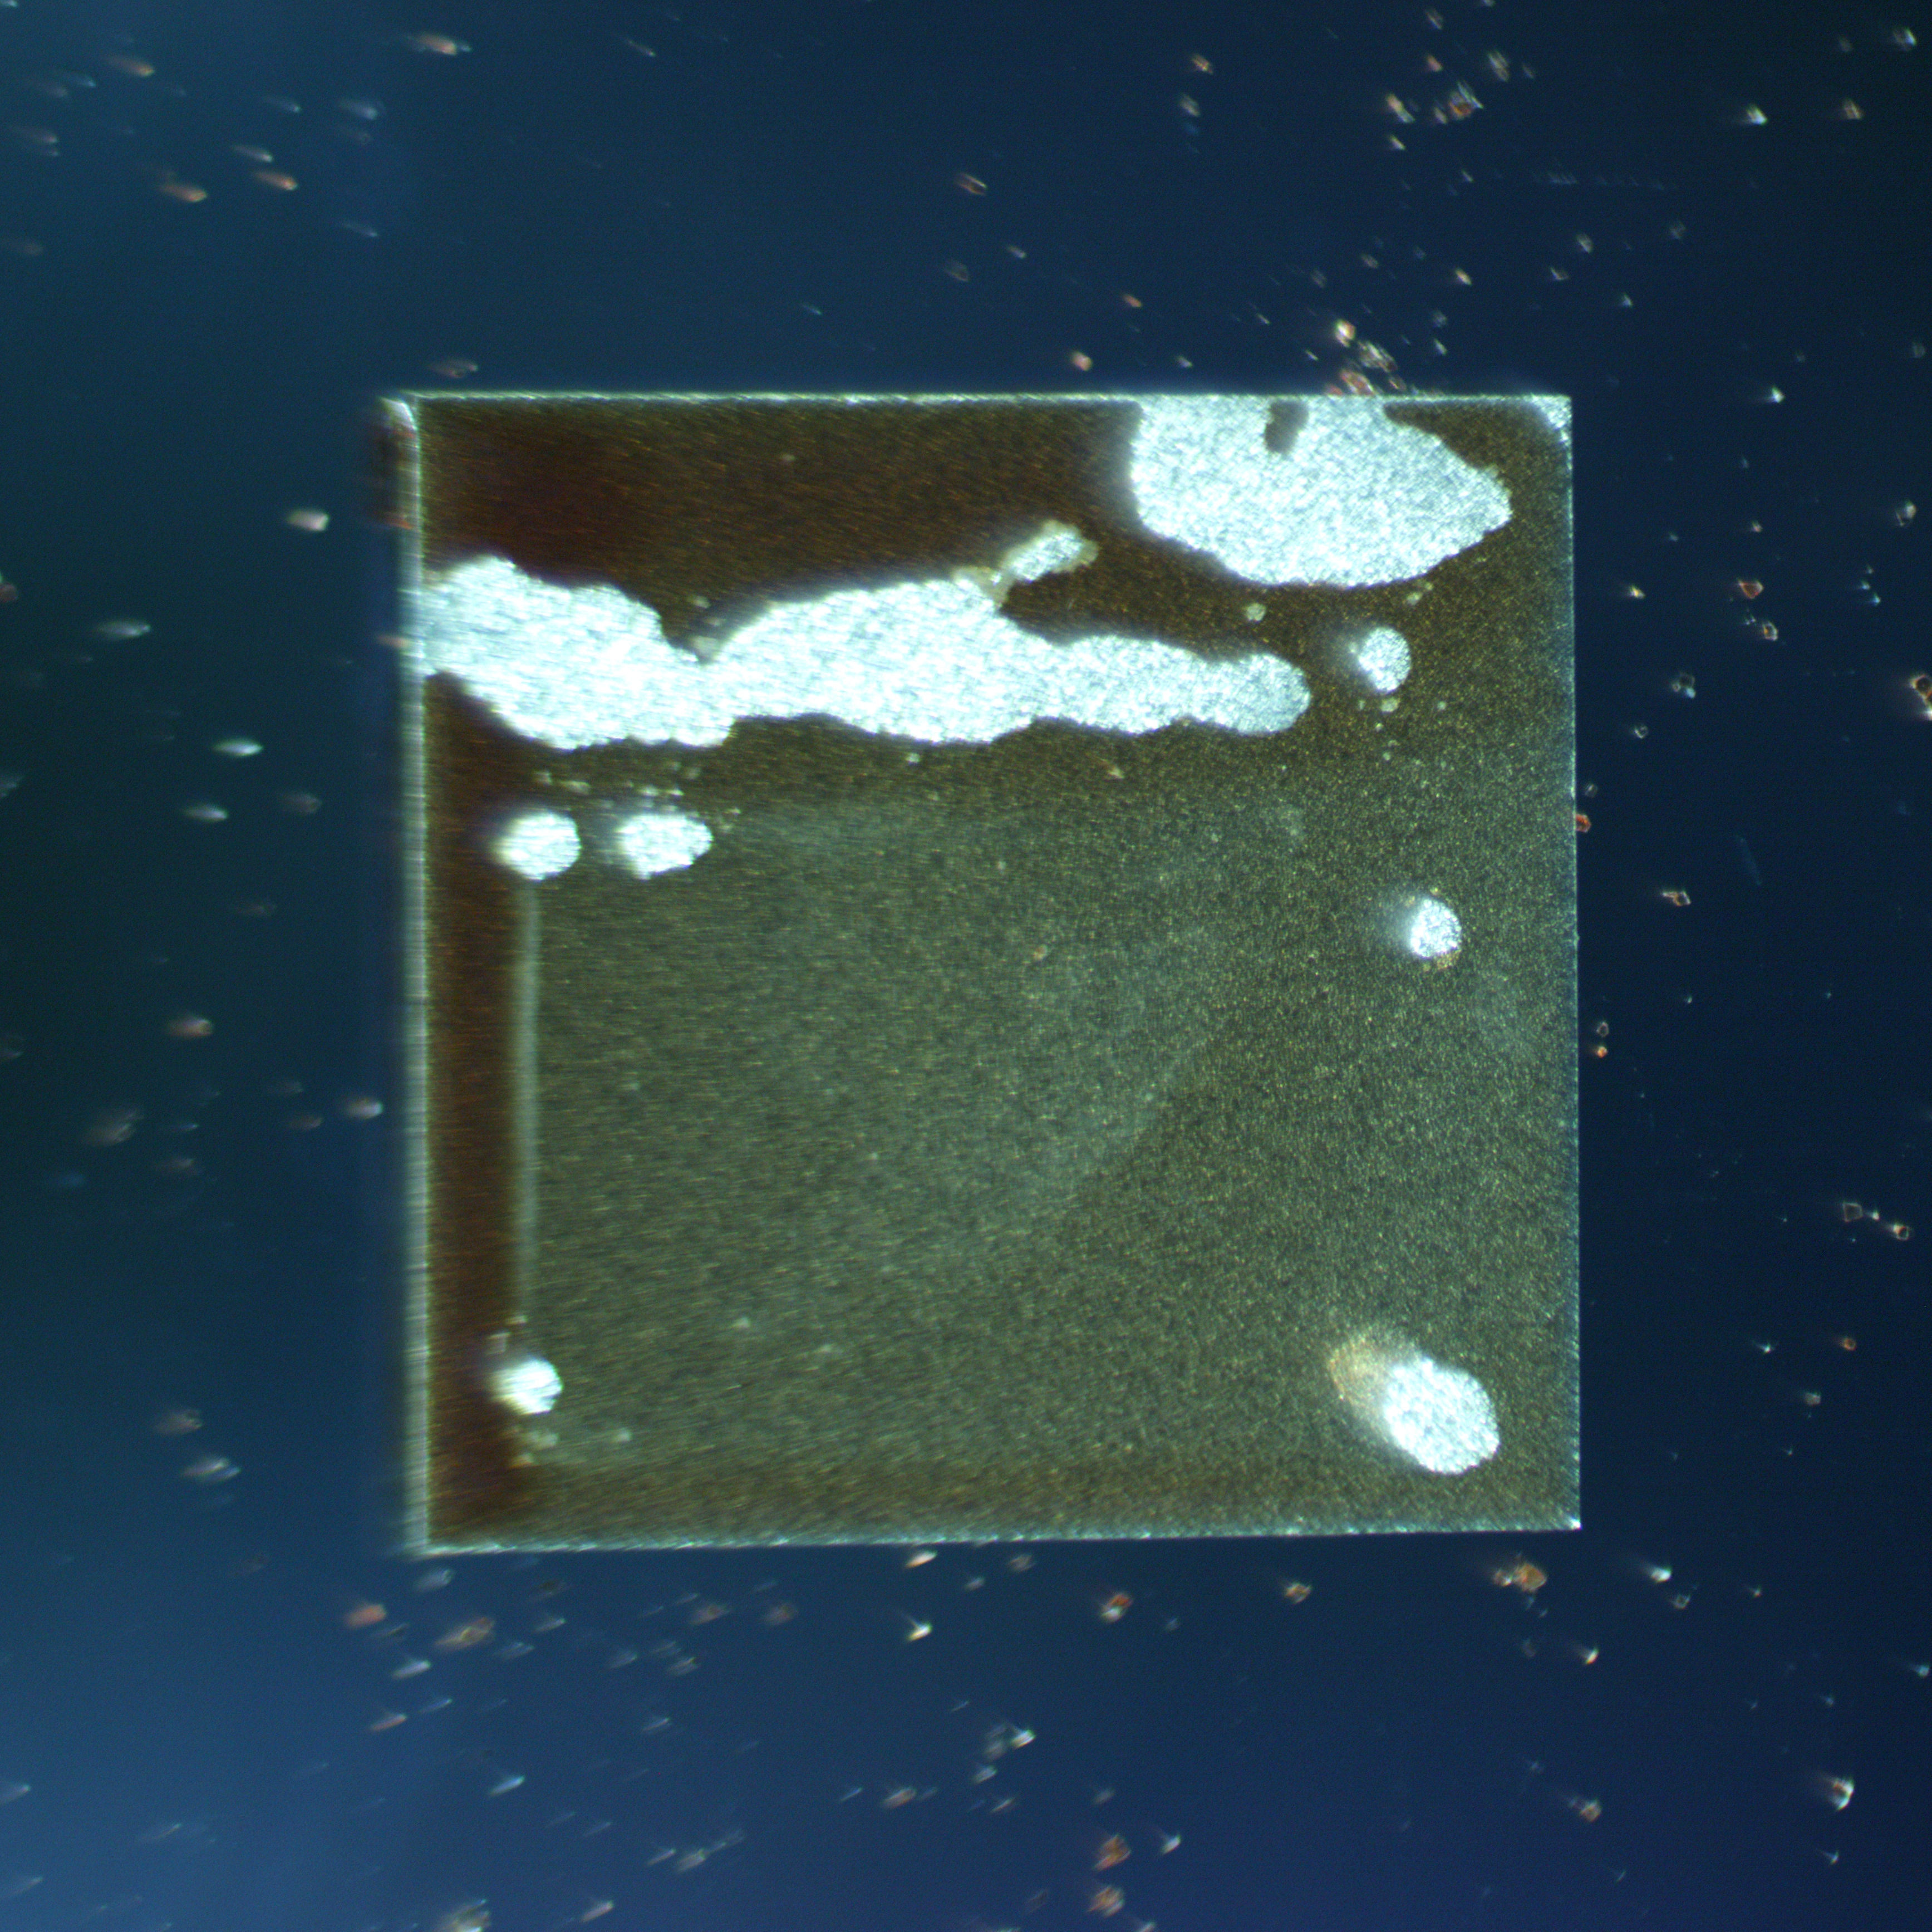
\includegraphics[width=\linewidth]{pics/spincoat/no10/10101.jpg}
        \caption{\textcolor{blue!60!black}{\textbf{Heater 1}}}
    \end{subfigure}
    \hfill
    \begin{subfigure}[t]{0.3\textwidth}
        \centering
        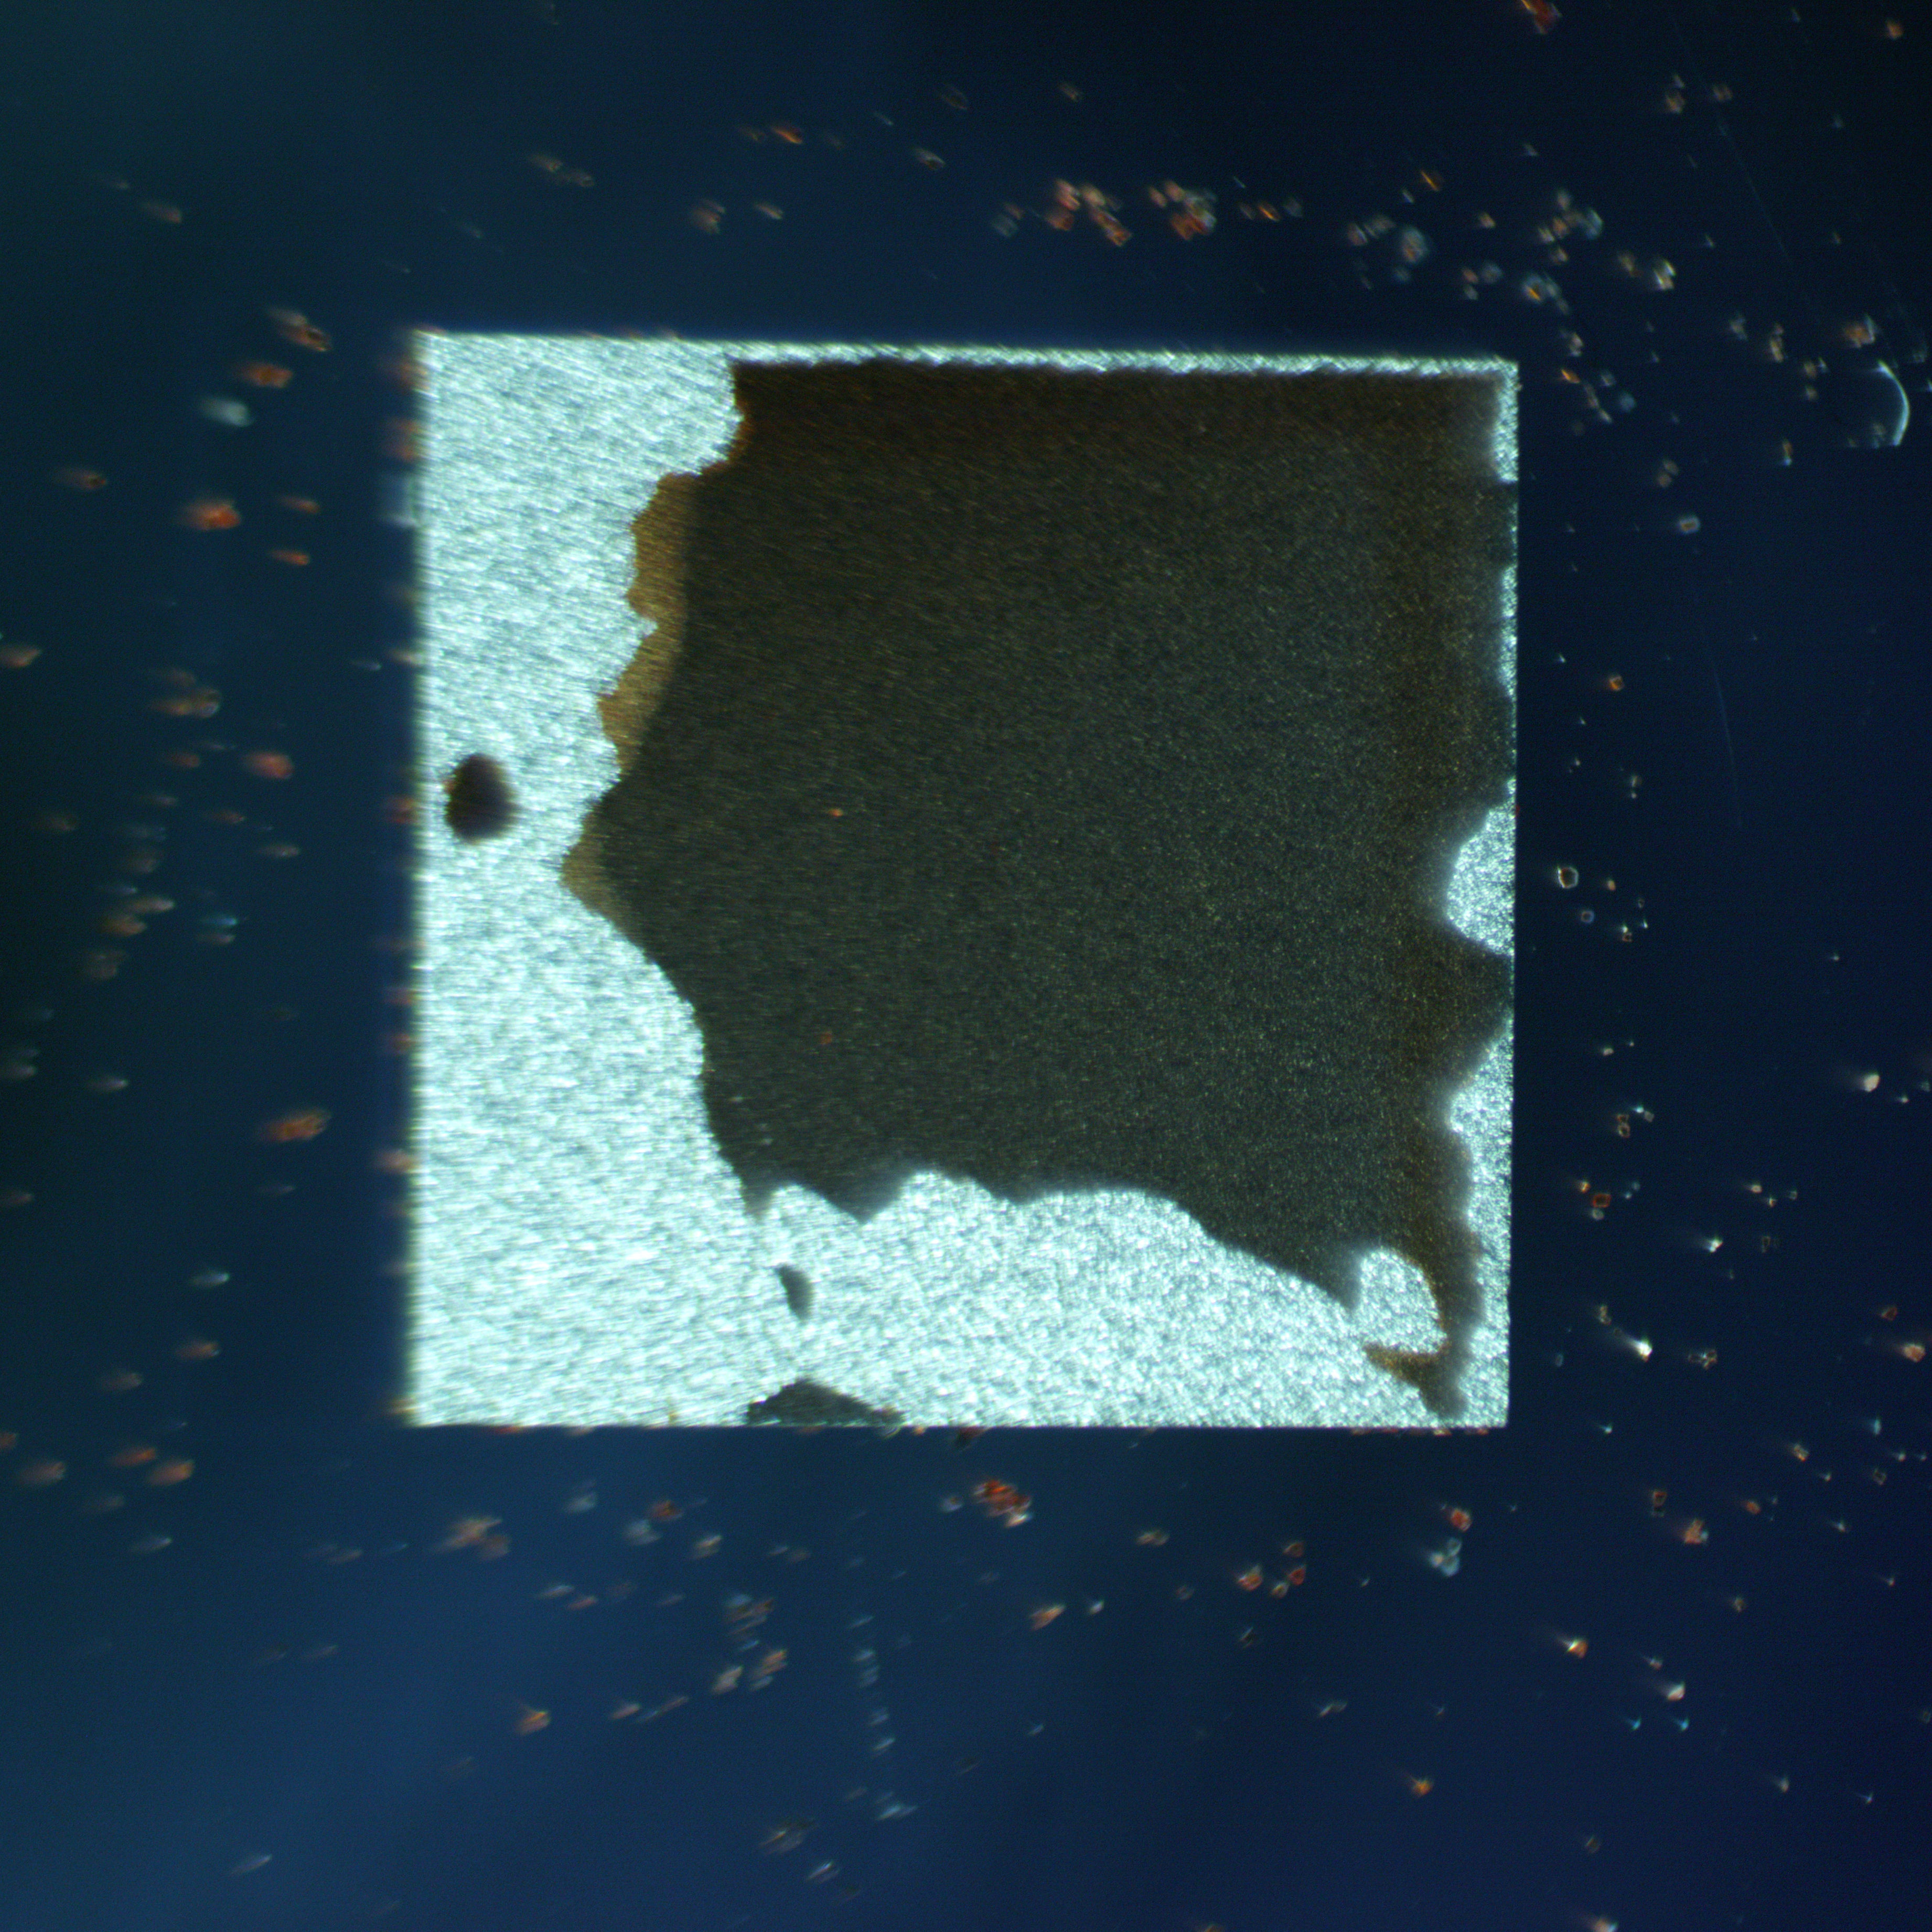
\includegraphics[width=\linewidth]{pics/spincoat/no10/10102.jpg}
        \caption{Heater 2}
    \end{subfigure}
    \hfill
    \begin{subfigure}[t]{0.3\textwidth}
        \centering
        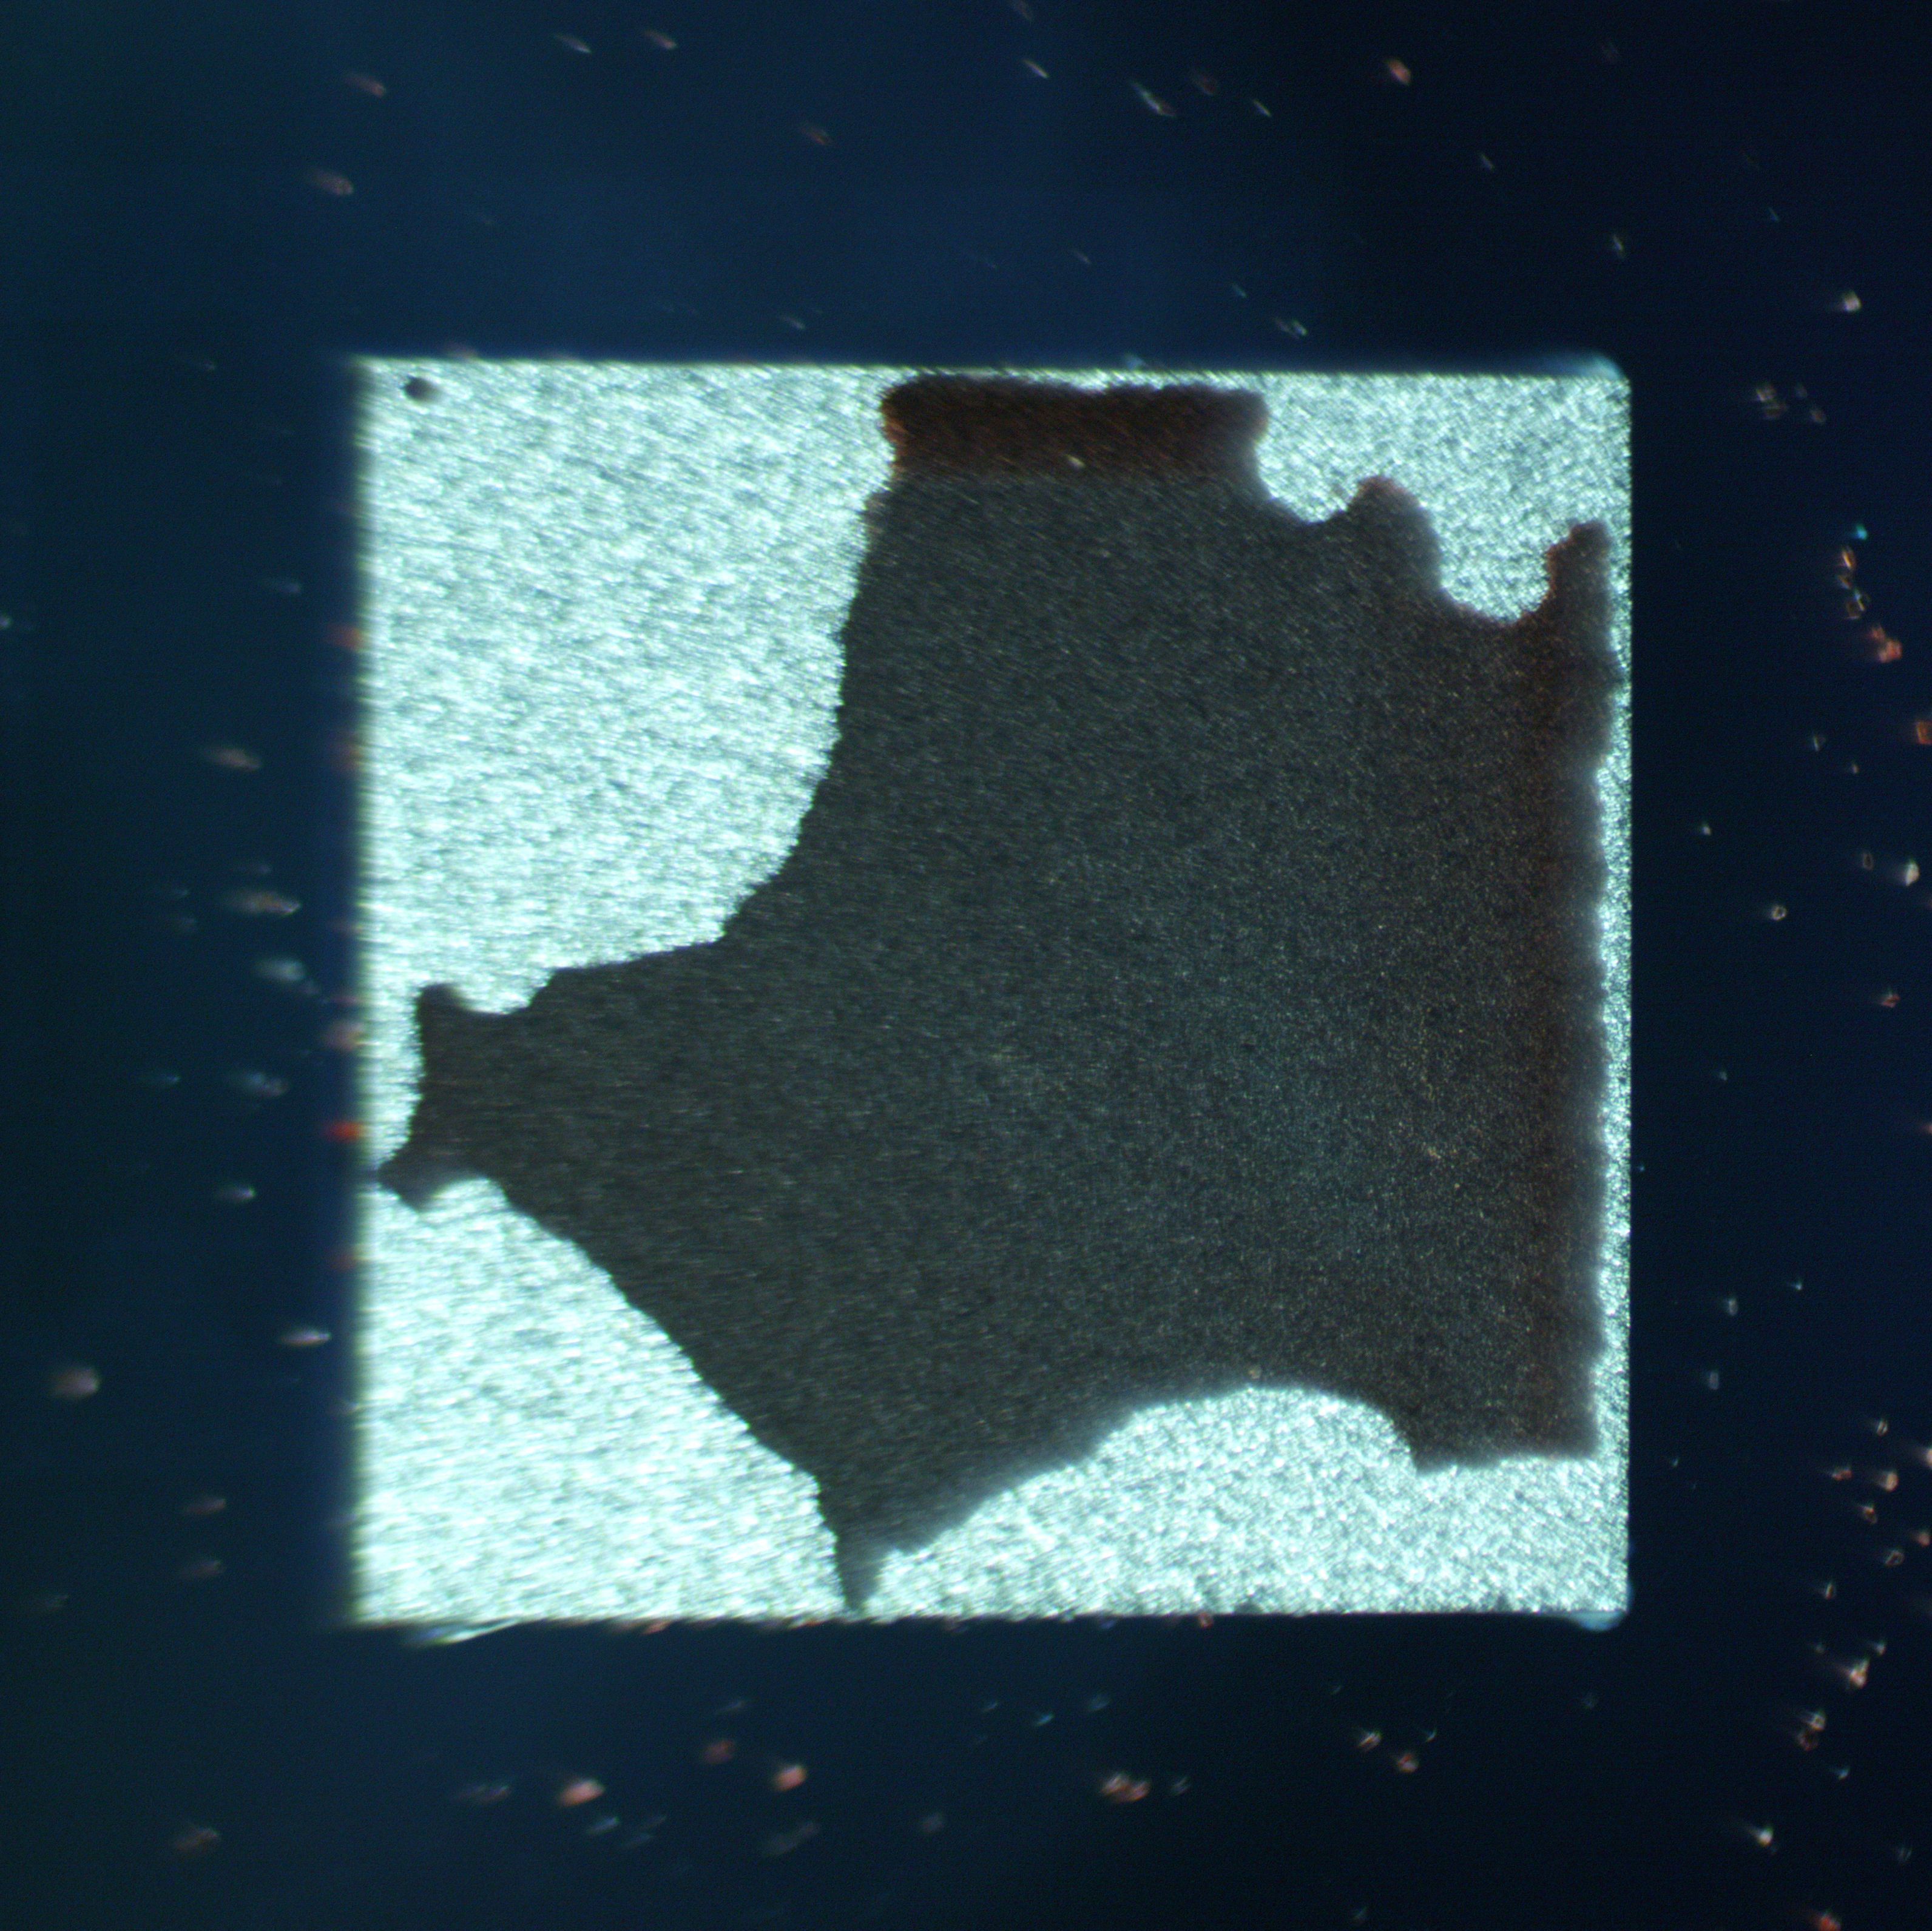
\includegraphics[width=\linewidth]{pics/spincoat/no10/10103.jpg}
        \caption{Heater 3}
    \end{subfigure}

    \vspace{0.8cm}

    % ---------- Row 2 ----------
    \begin{subfigure}[t]{0.3\textwidth}
        \centering
        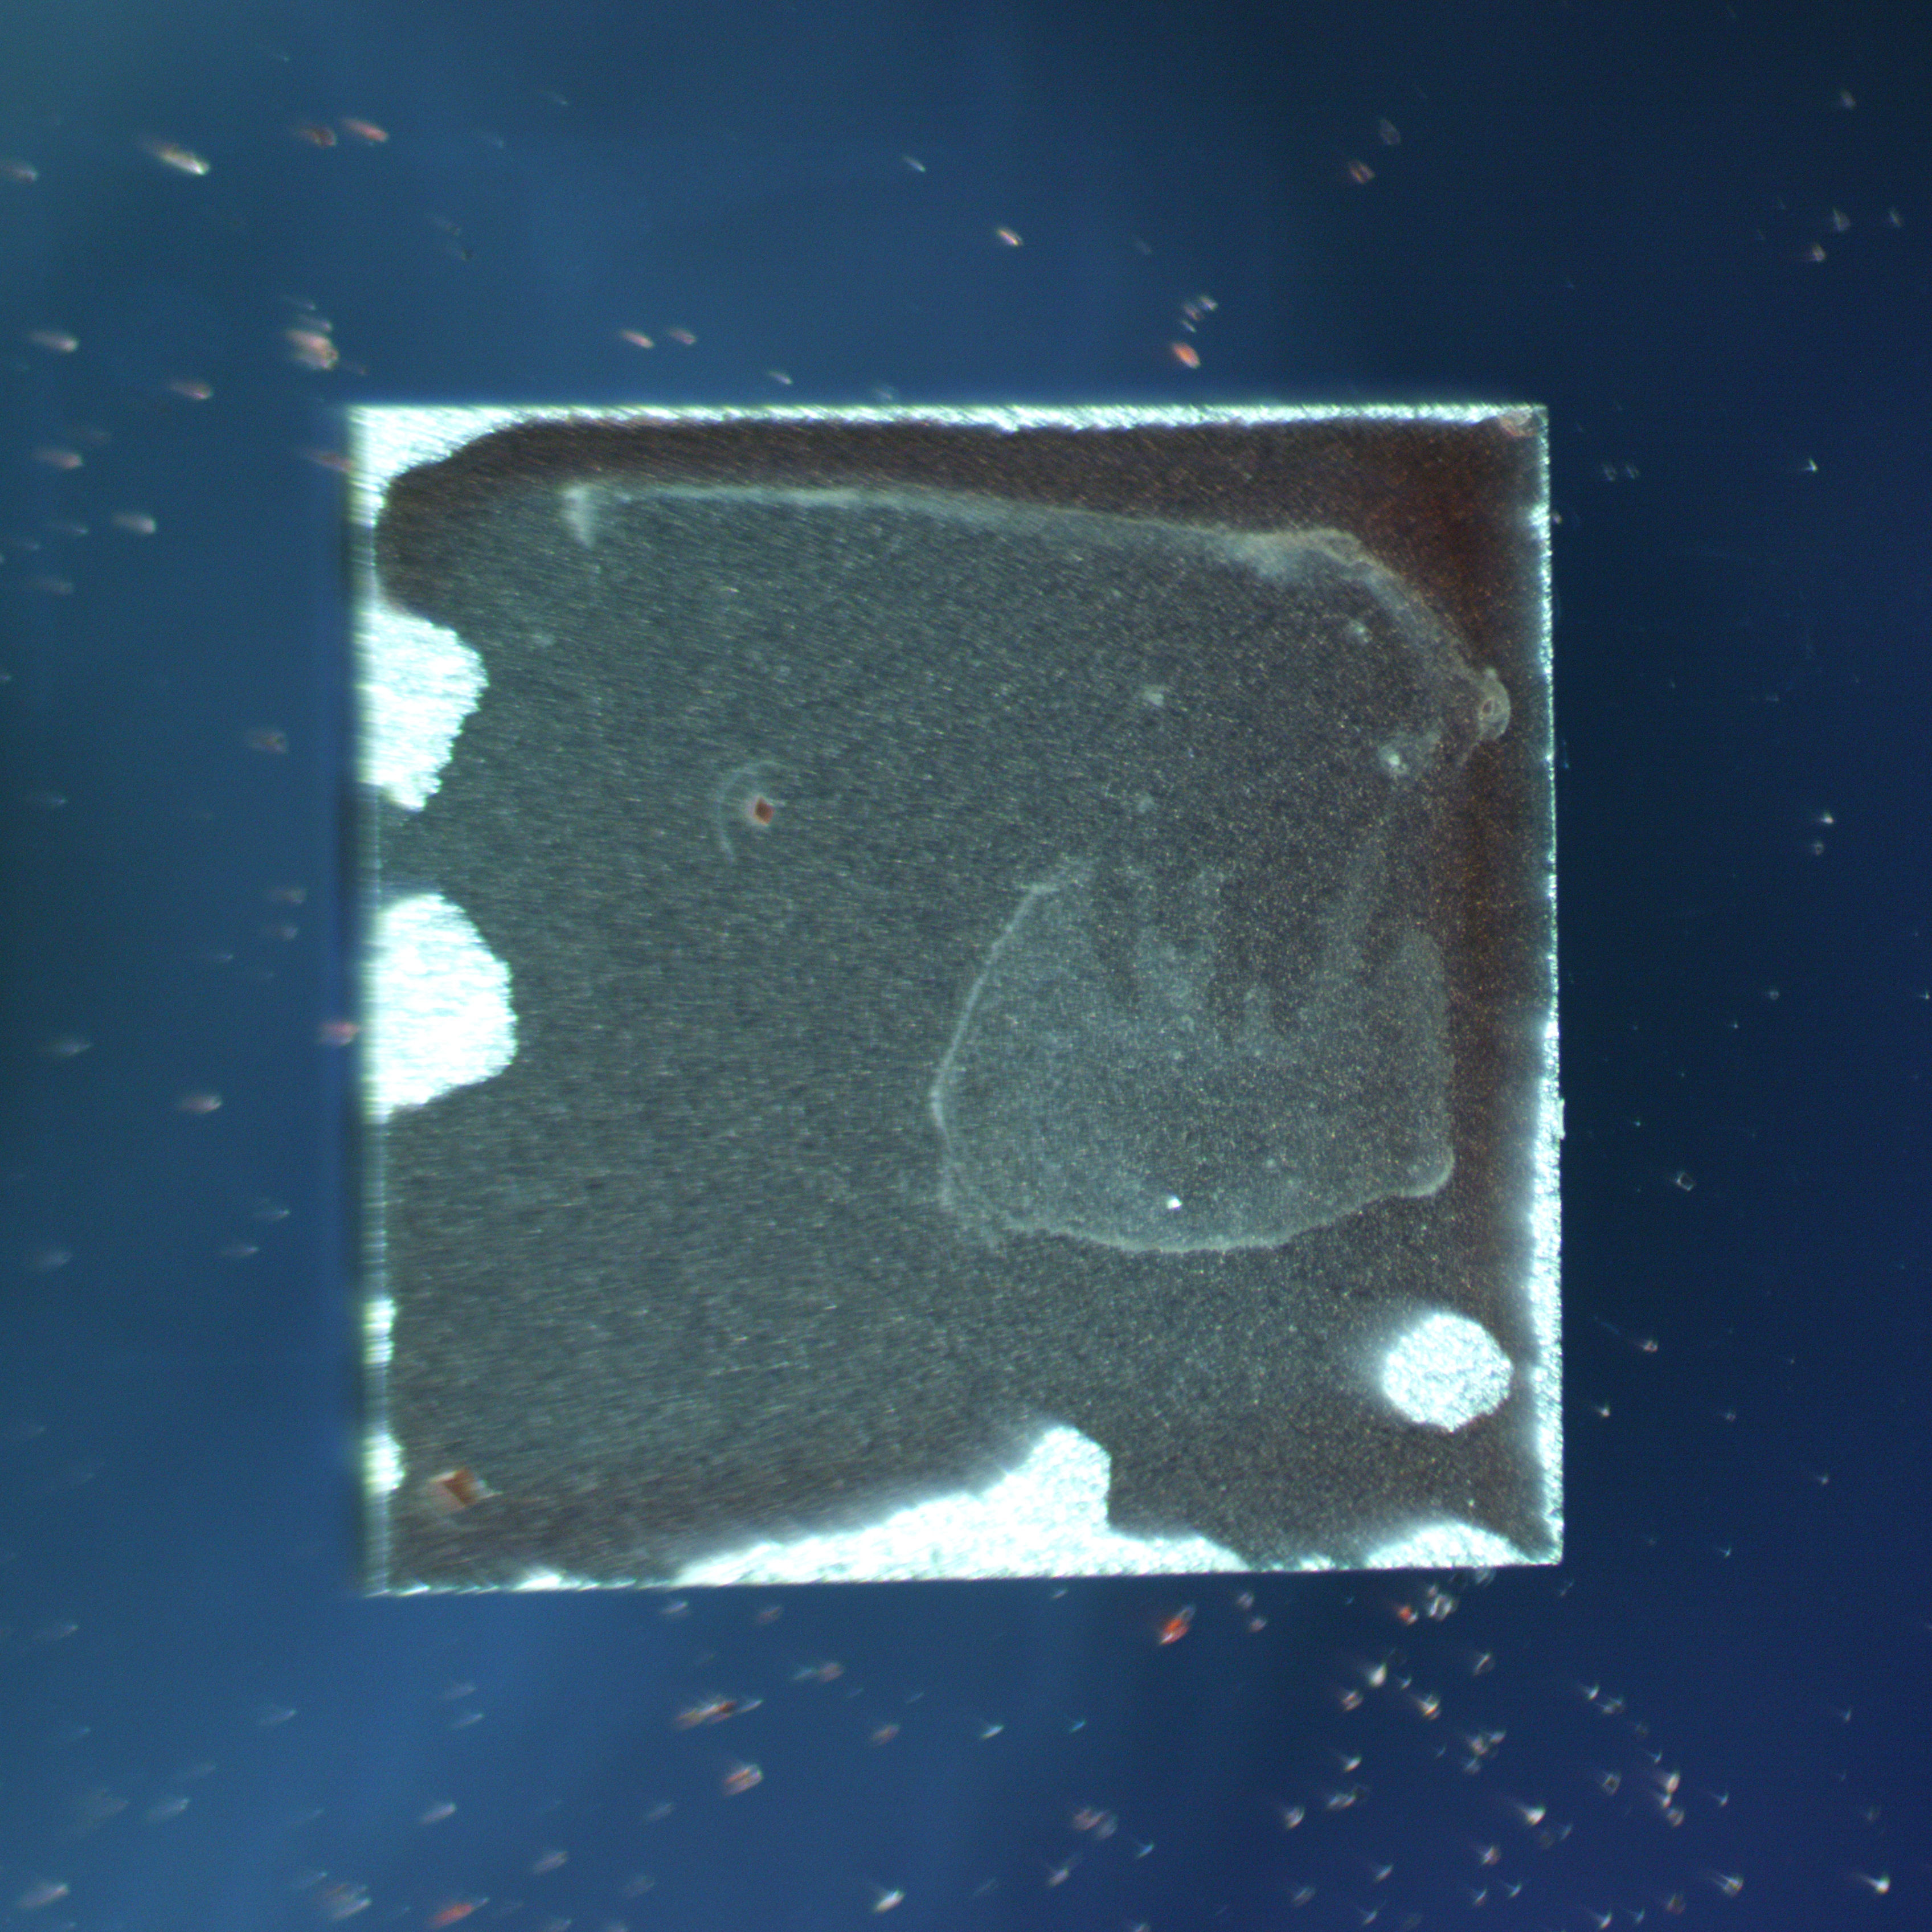
\includegraphics[width=\linewidth]{pics/spincoat/no10/10104.jpg}
        \caption{\textcolor{blue!60!black}{\textbf{Heater 4}}}
    \end{subfigure}
    \hfill
    \begin{subfigure}[t]{0.3\textwidth}
        \centering
        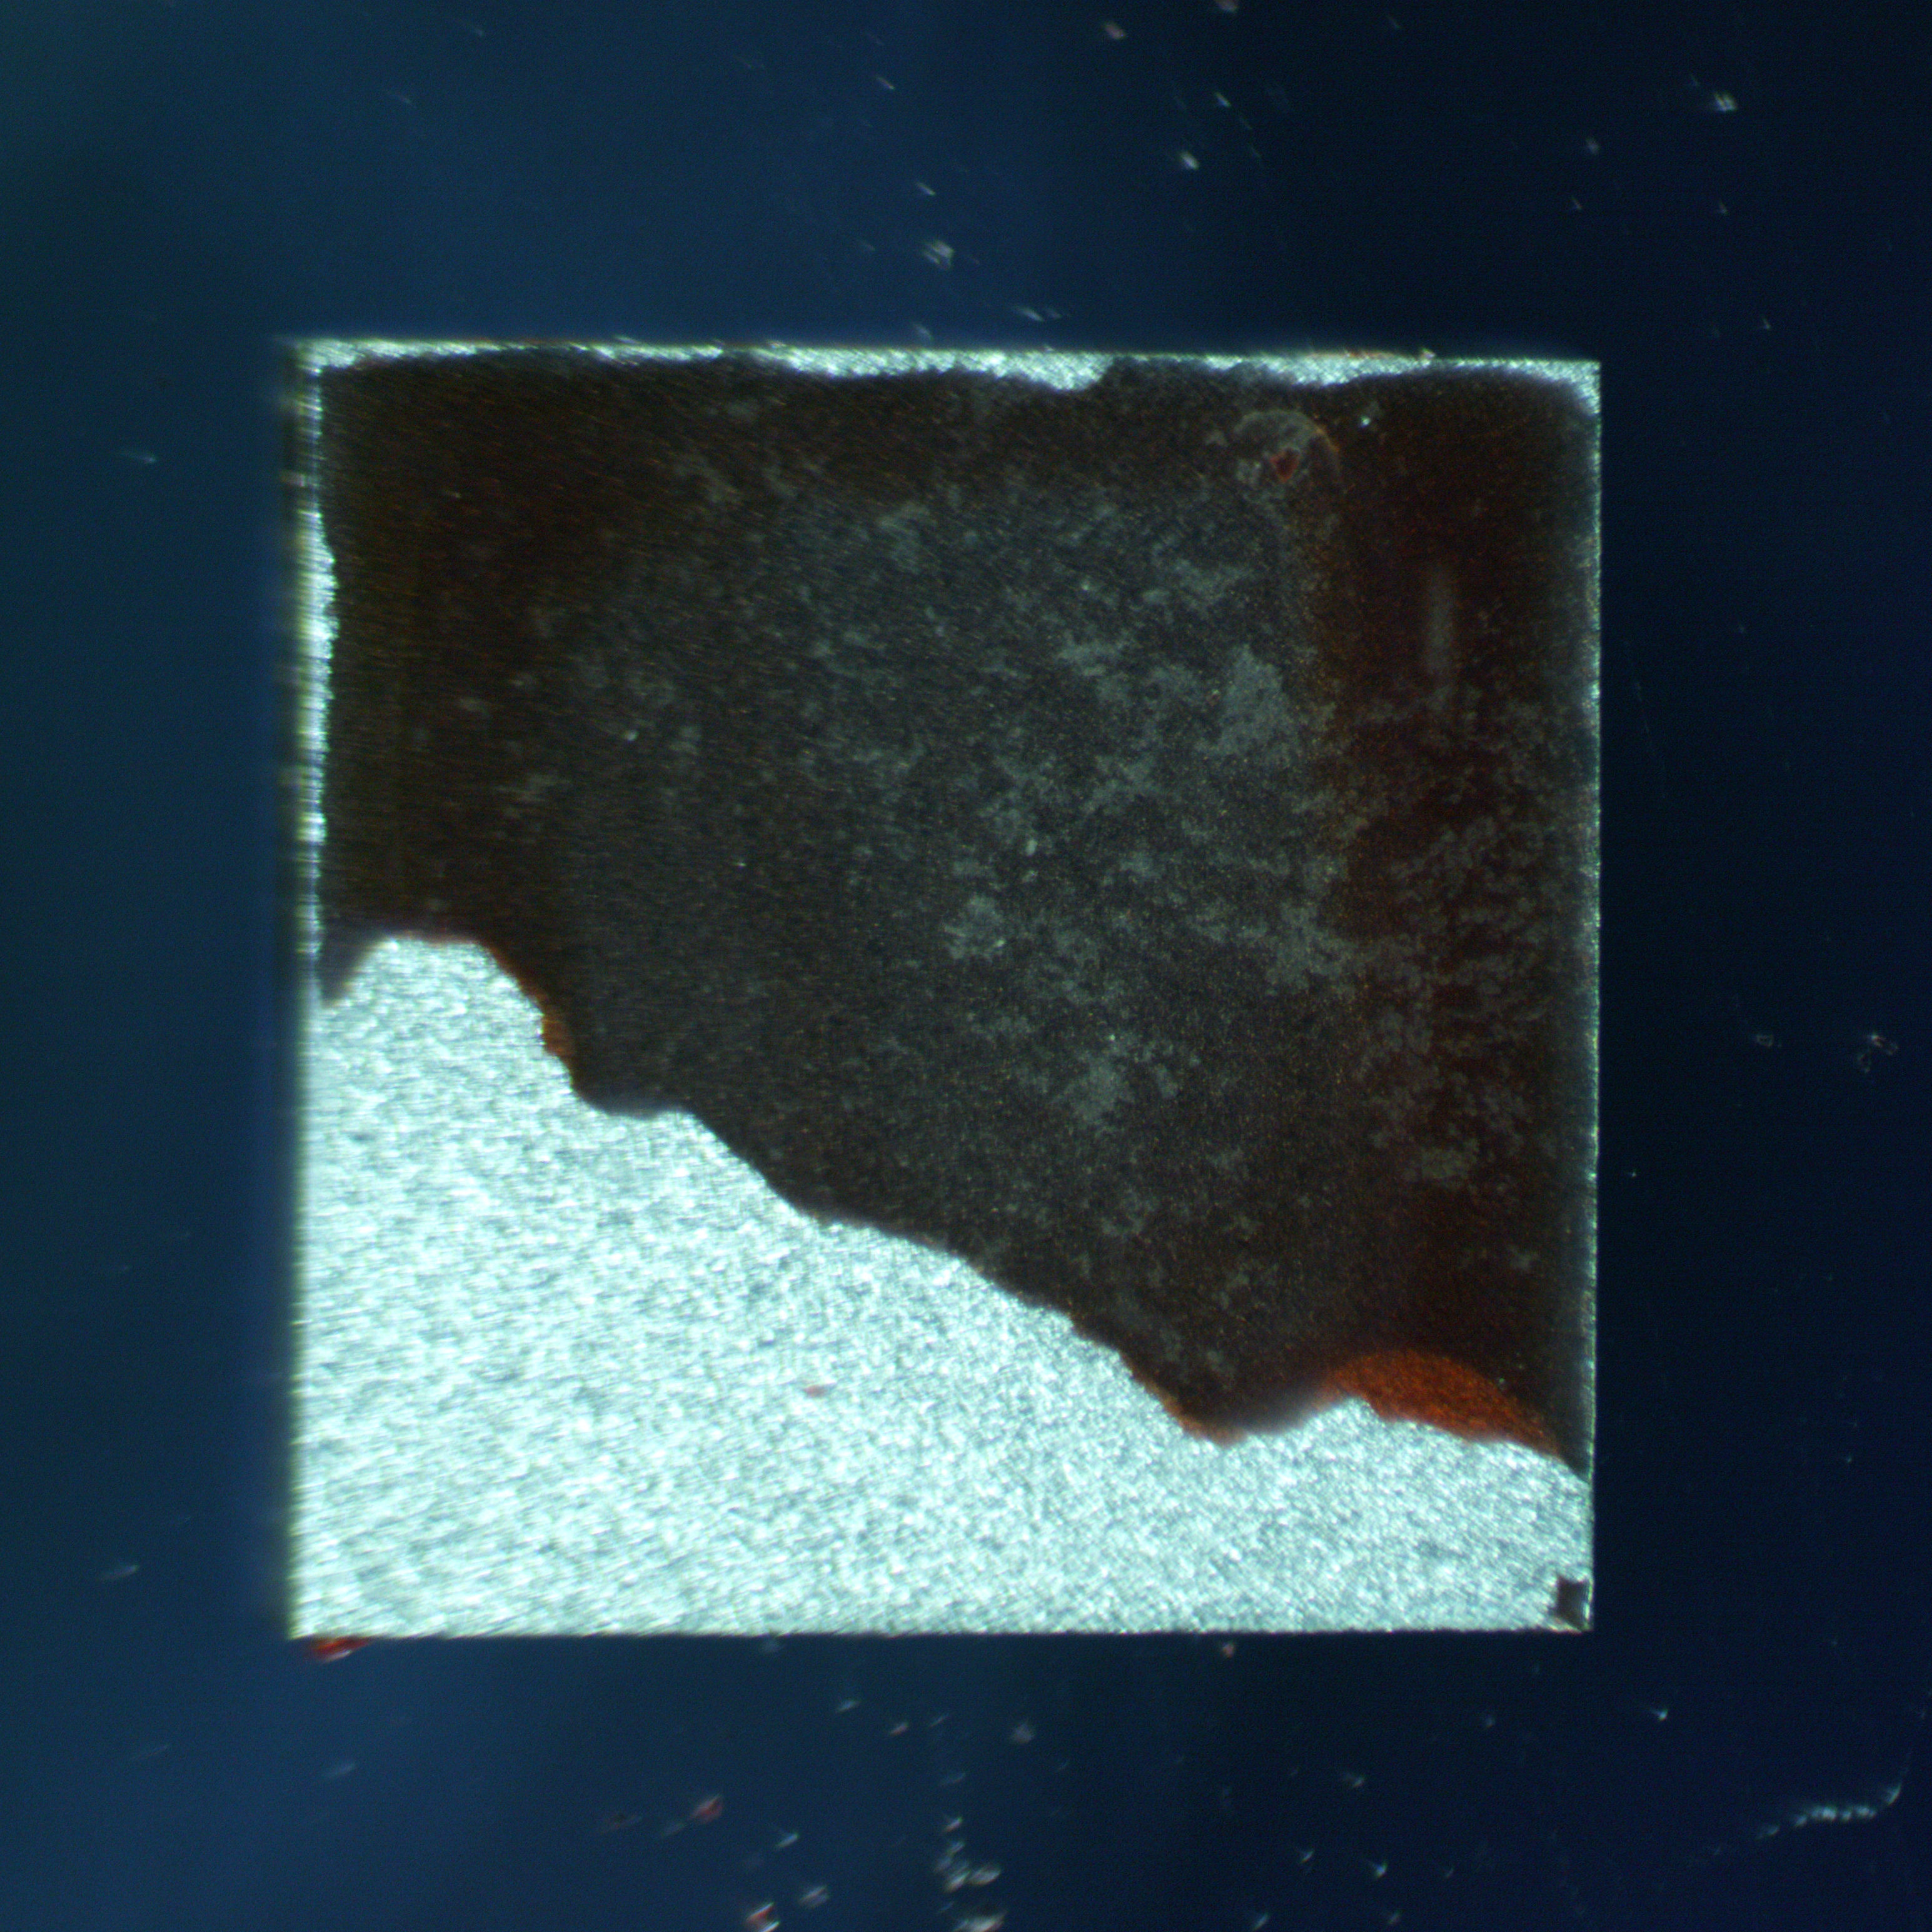
\includegraphics[width=\linewidth]{pics/spincoat/no10/10105.jpg}
        \caption{\textcolor{blue!60!black}{\textbf{Heater 5}}}
    \end{subfigure}
    \hfill
    \begin{subfigure}[t]{0.3\textwidth}
        \centering
        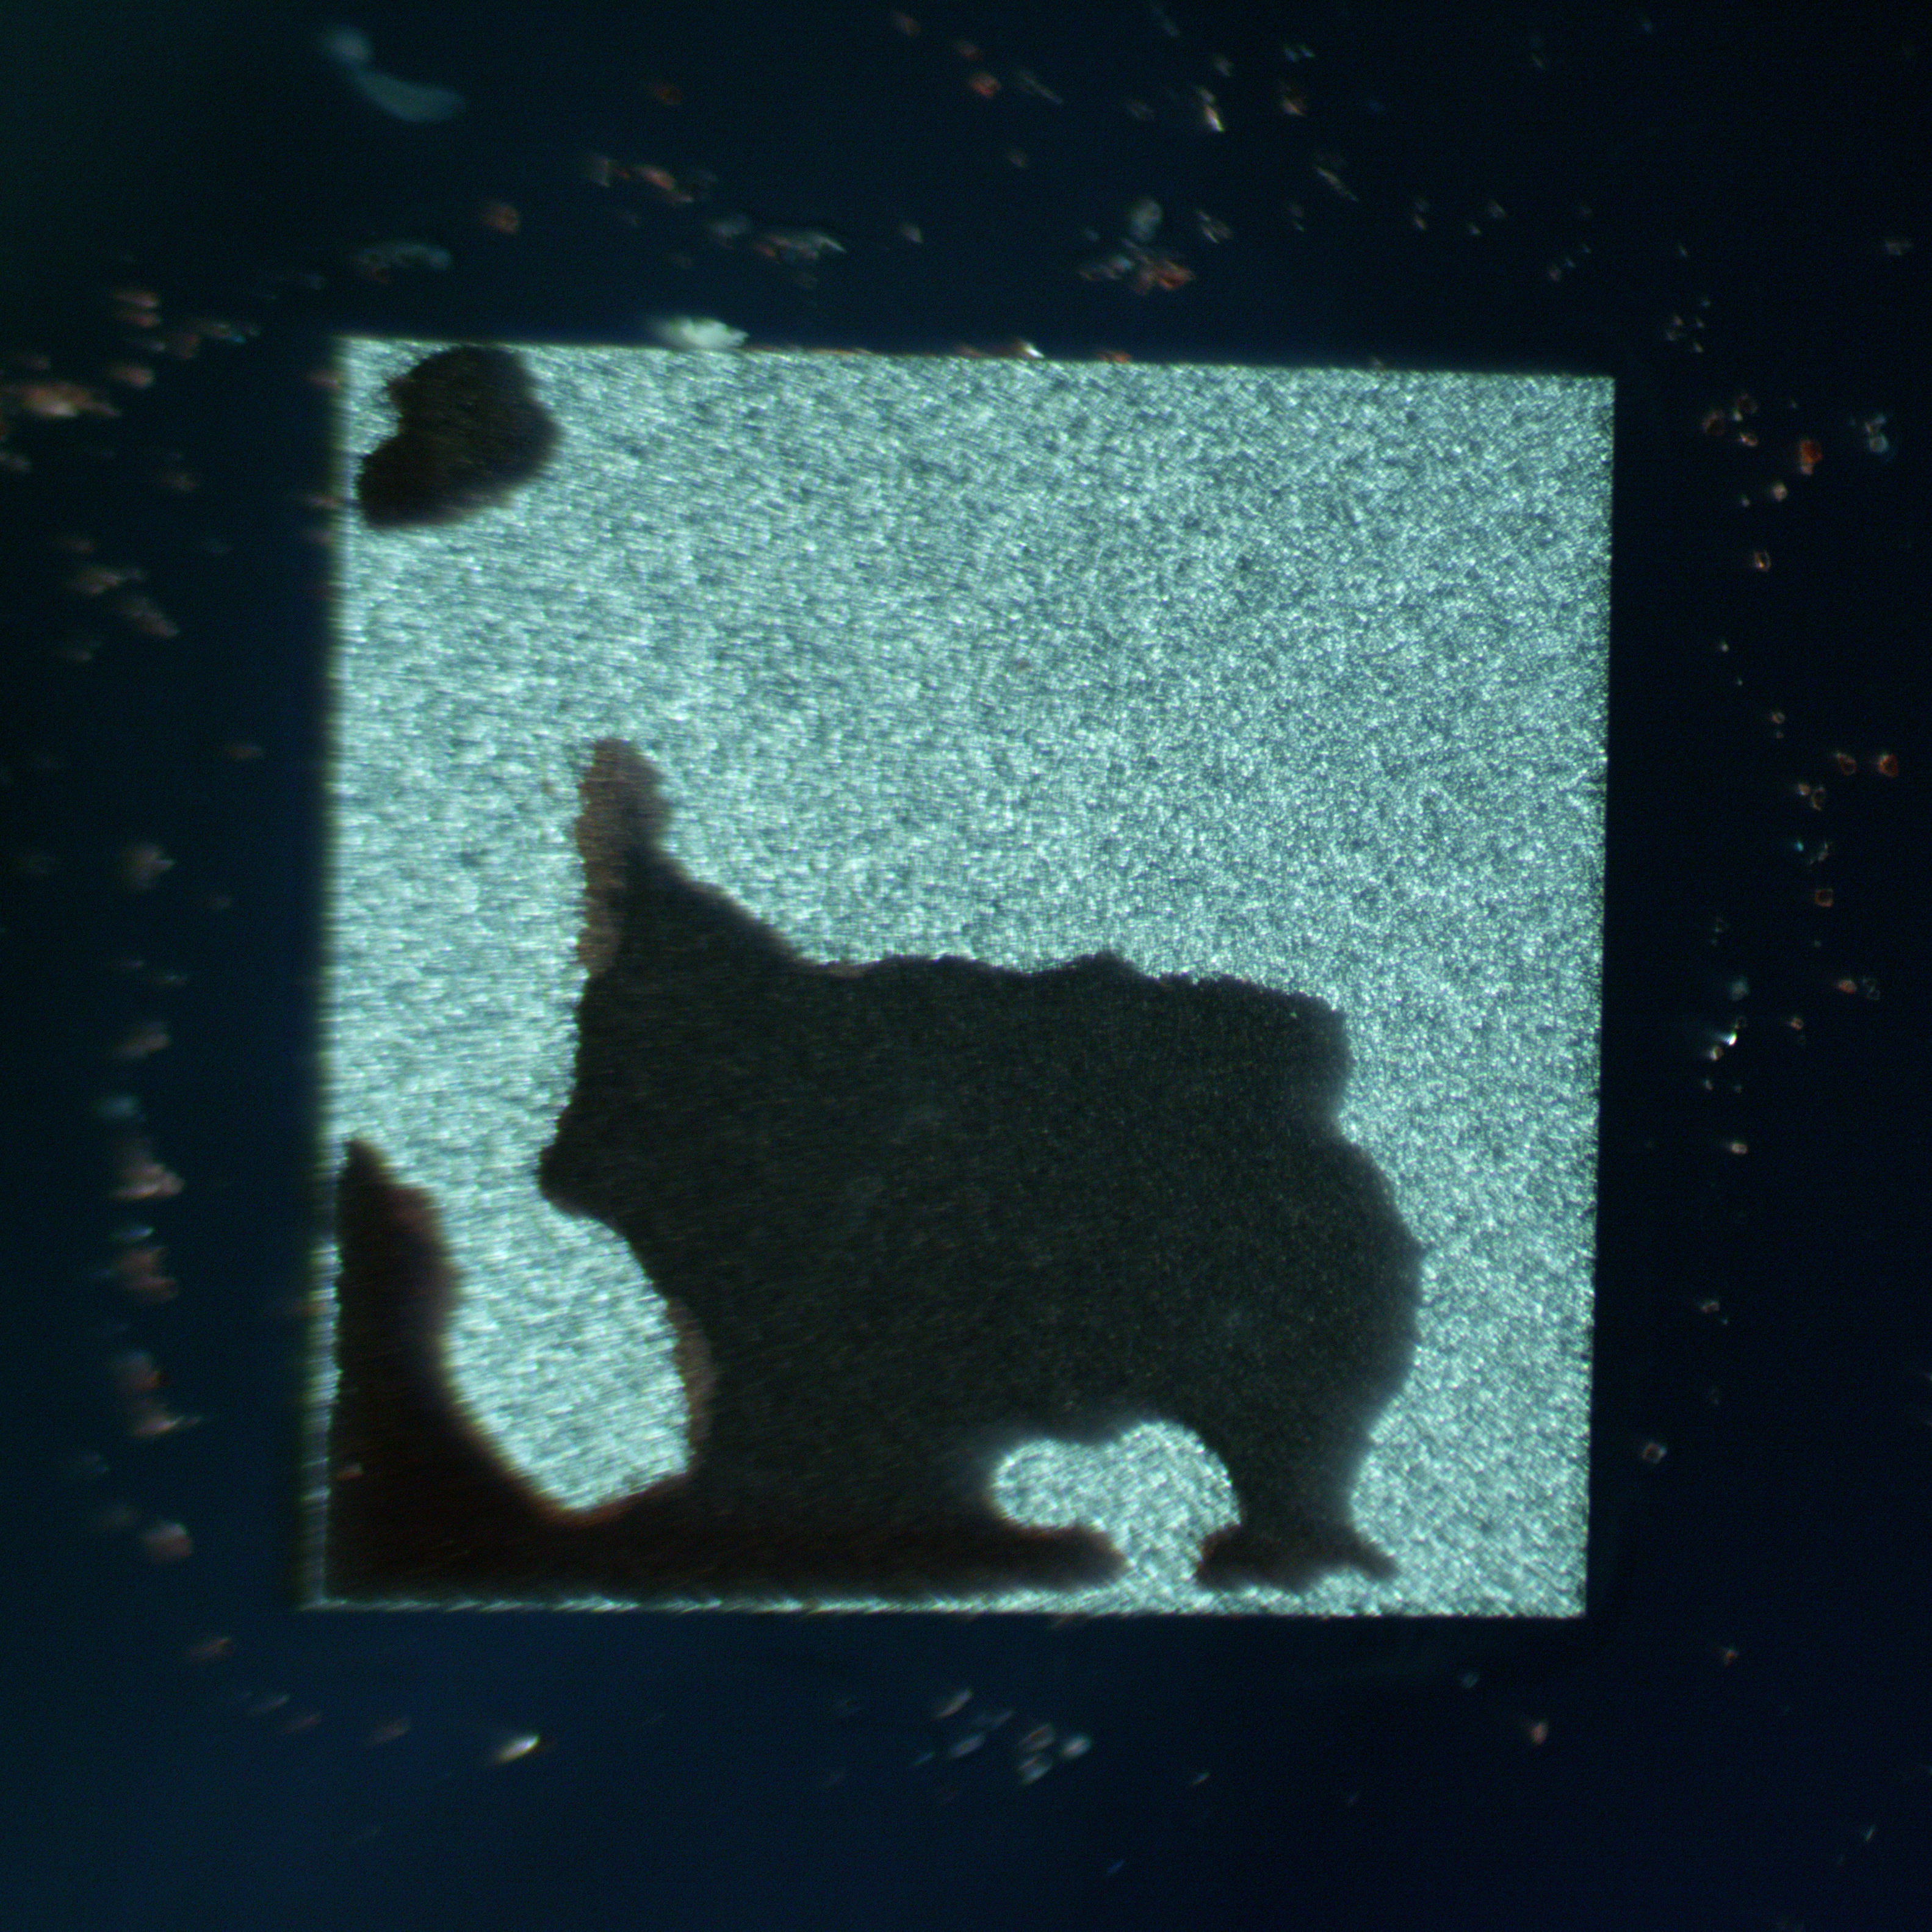
\includegraphics[width=\linewidth]{pics/spincoat/no10/10106.jpg}
        \caption{Heater 6}
    \end{subfigure}

    \vspace{0.8cm}

    % ---------- Row 3 ----------
    \begin{subfigure}[t]{0.3\textwidth}
        \centering
        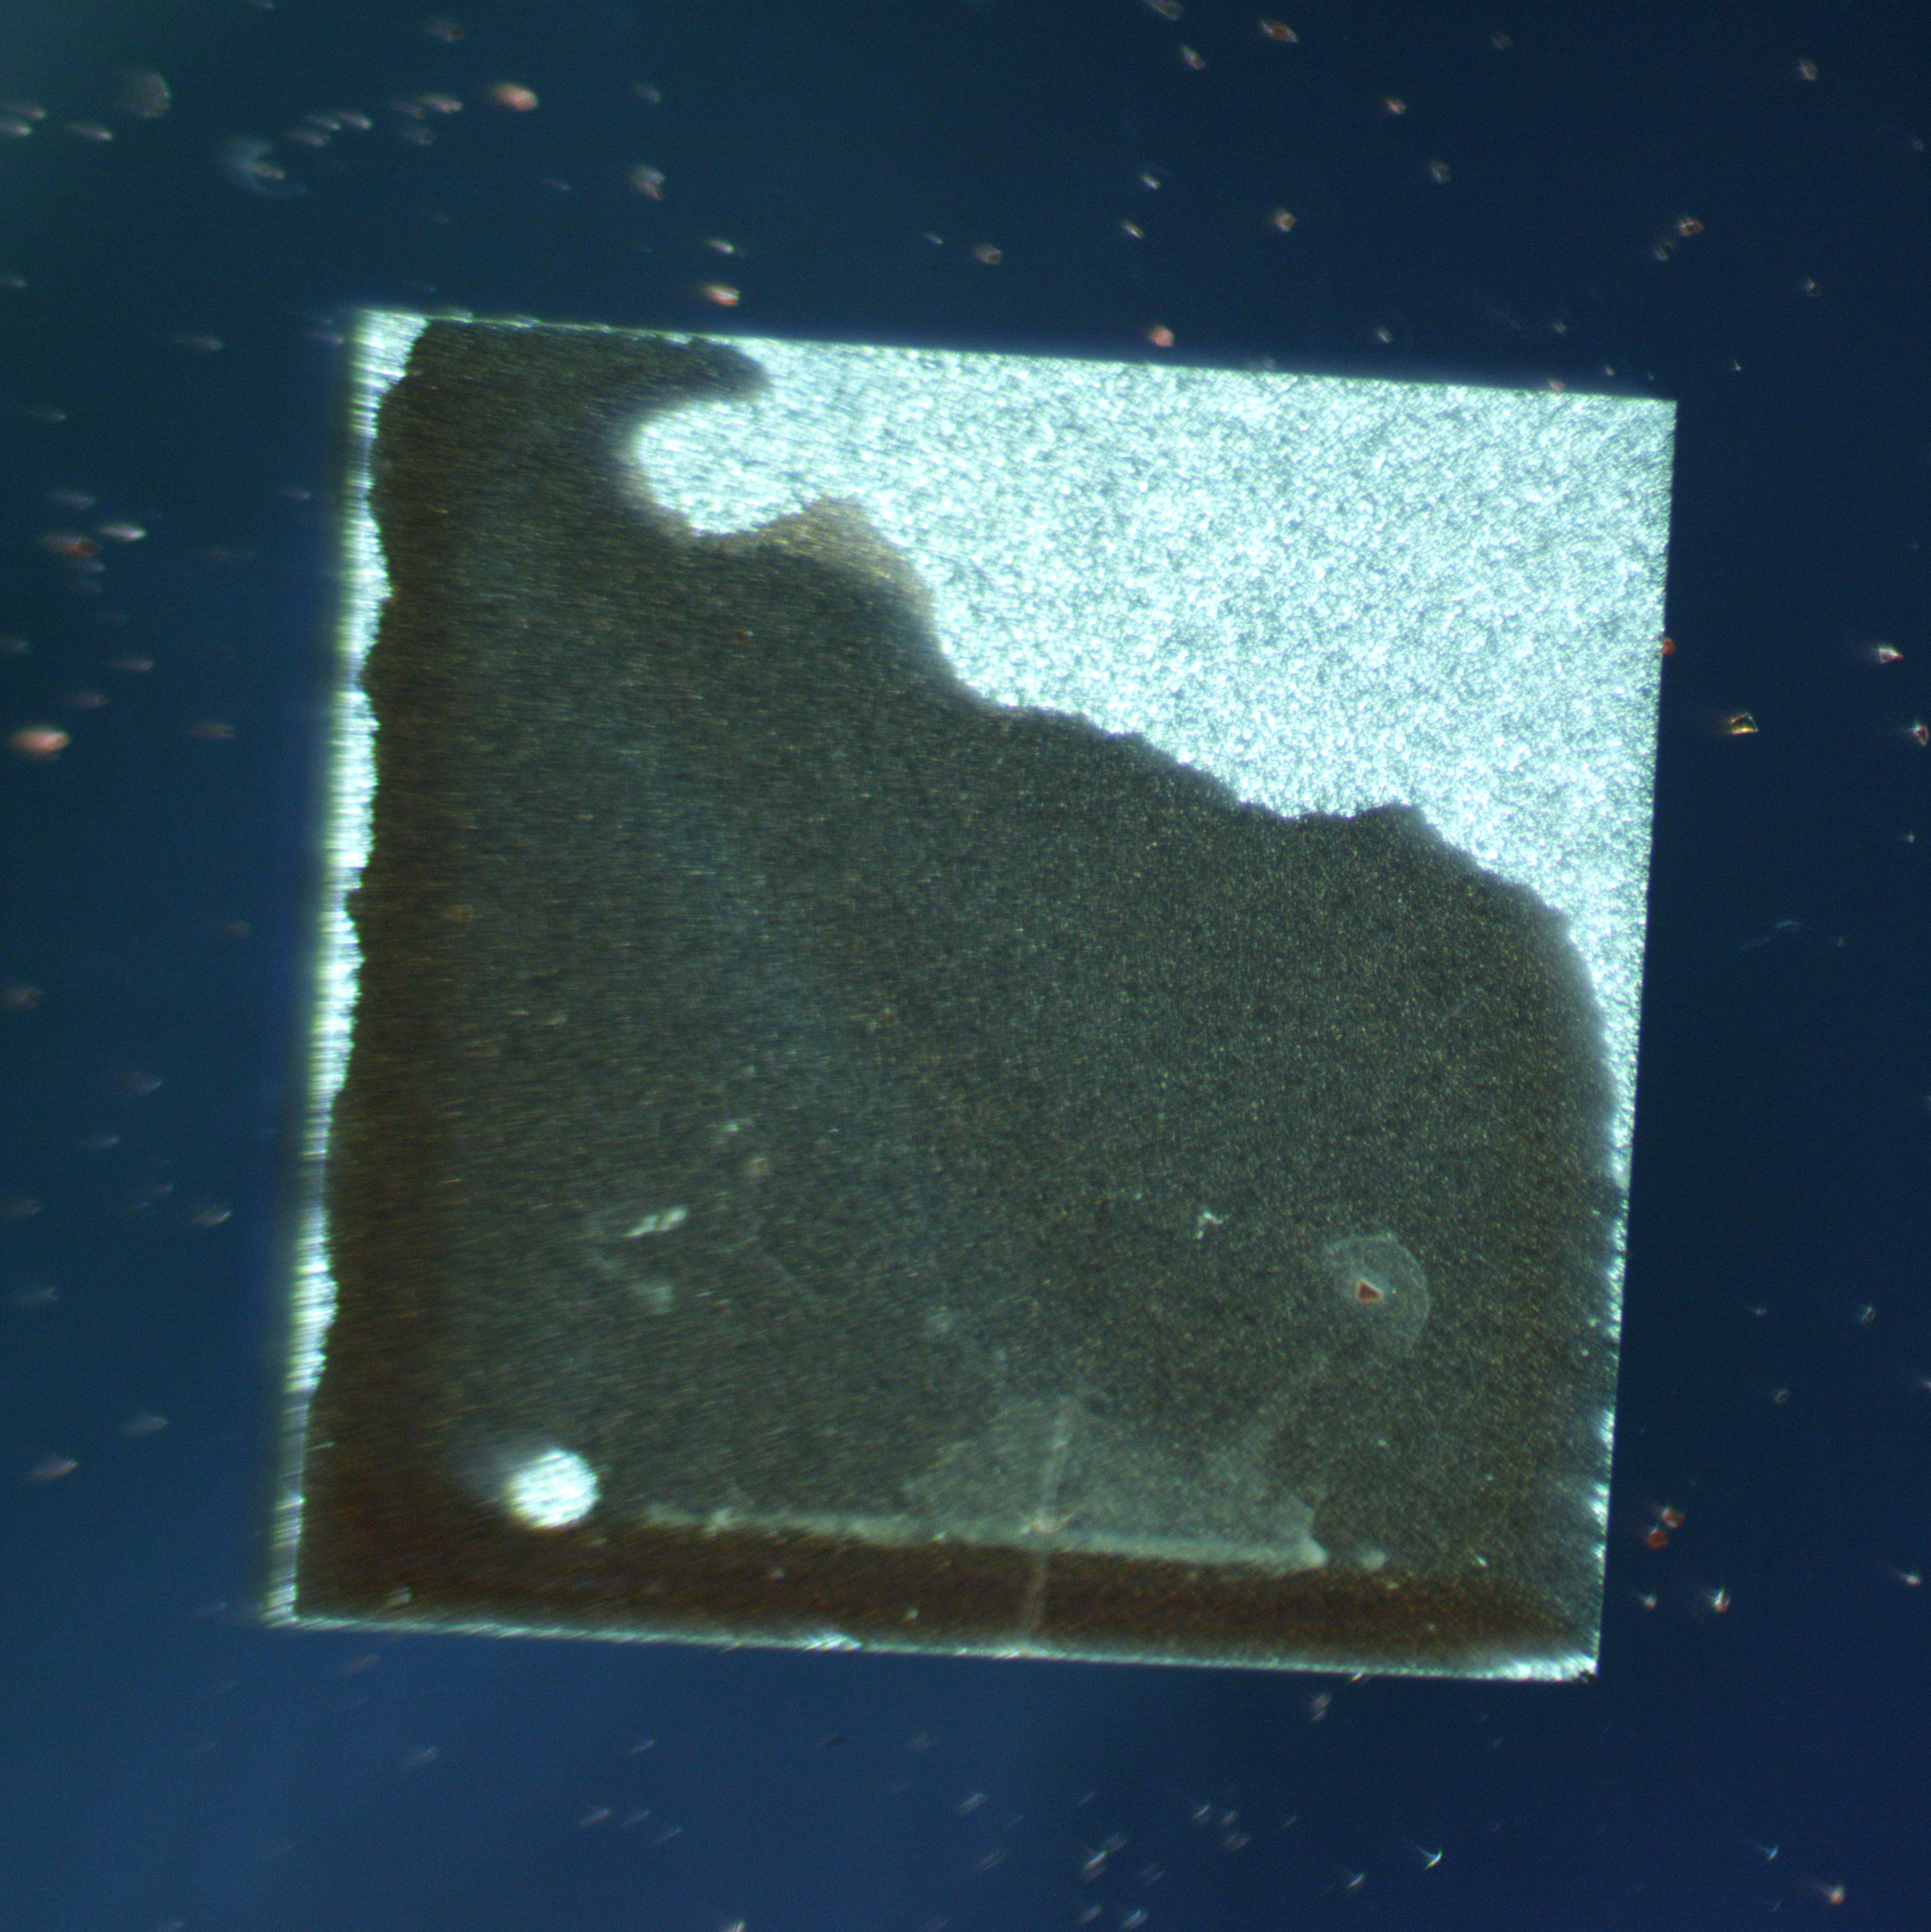
\includegraphics[width=\linewidth]{pics/spincoat/no10/10107.jpg}
        \caption{\textcolor{blue!60!black}{\textbf{Heater 7}}}
    \end{subfigure}
    \hfill
    \begin{subfigure}[t]{0.3\textwidth}
        \centering
        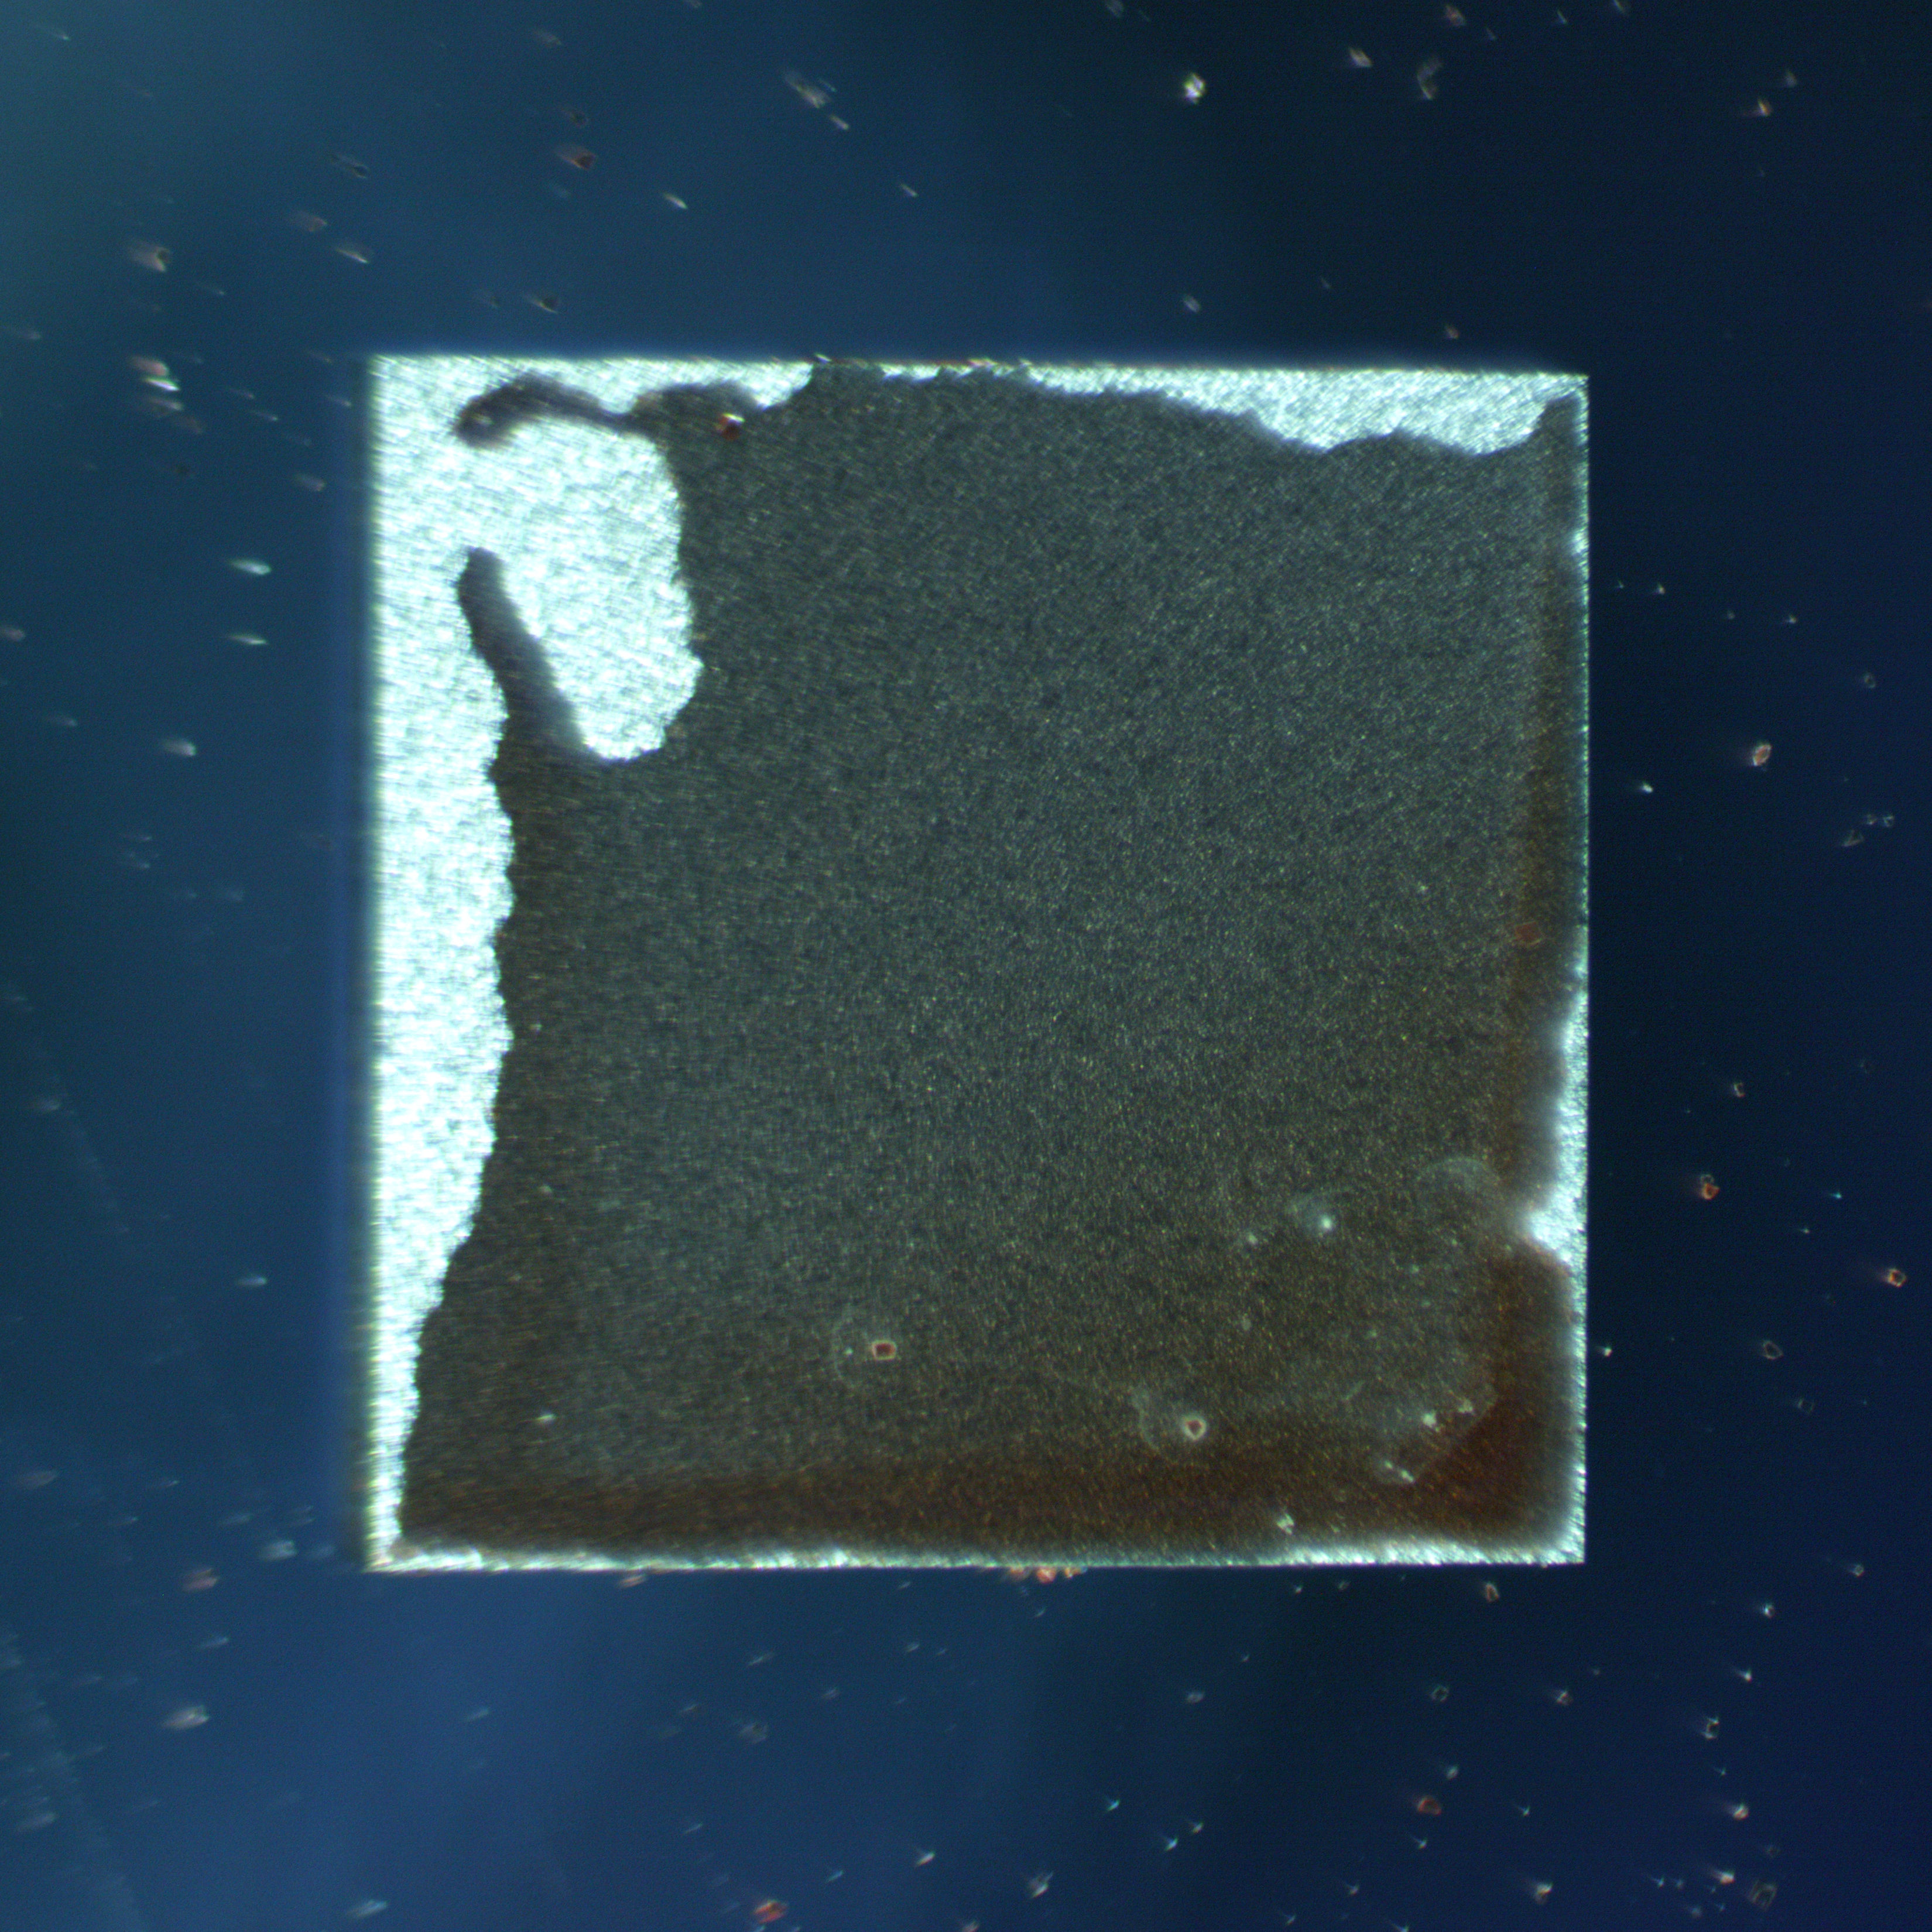
\includegraphics[width=\linewidth]{pics/spincoat/no10/10108.jpg}
        \caption{\textcolor{blue!60!black}{\textbf{Heater 8}}}
    \end{subfigure}
    \hfill
    \begin{subfigure}[t]{0.3\textwidth}
        \centering
        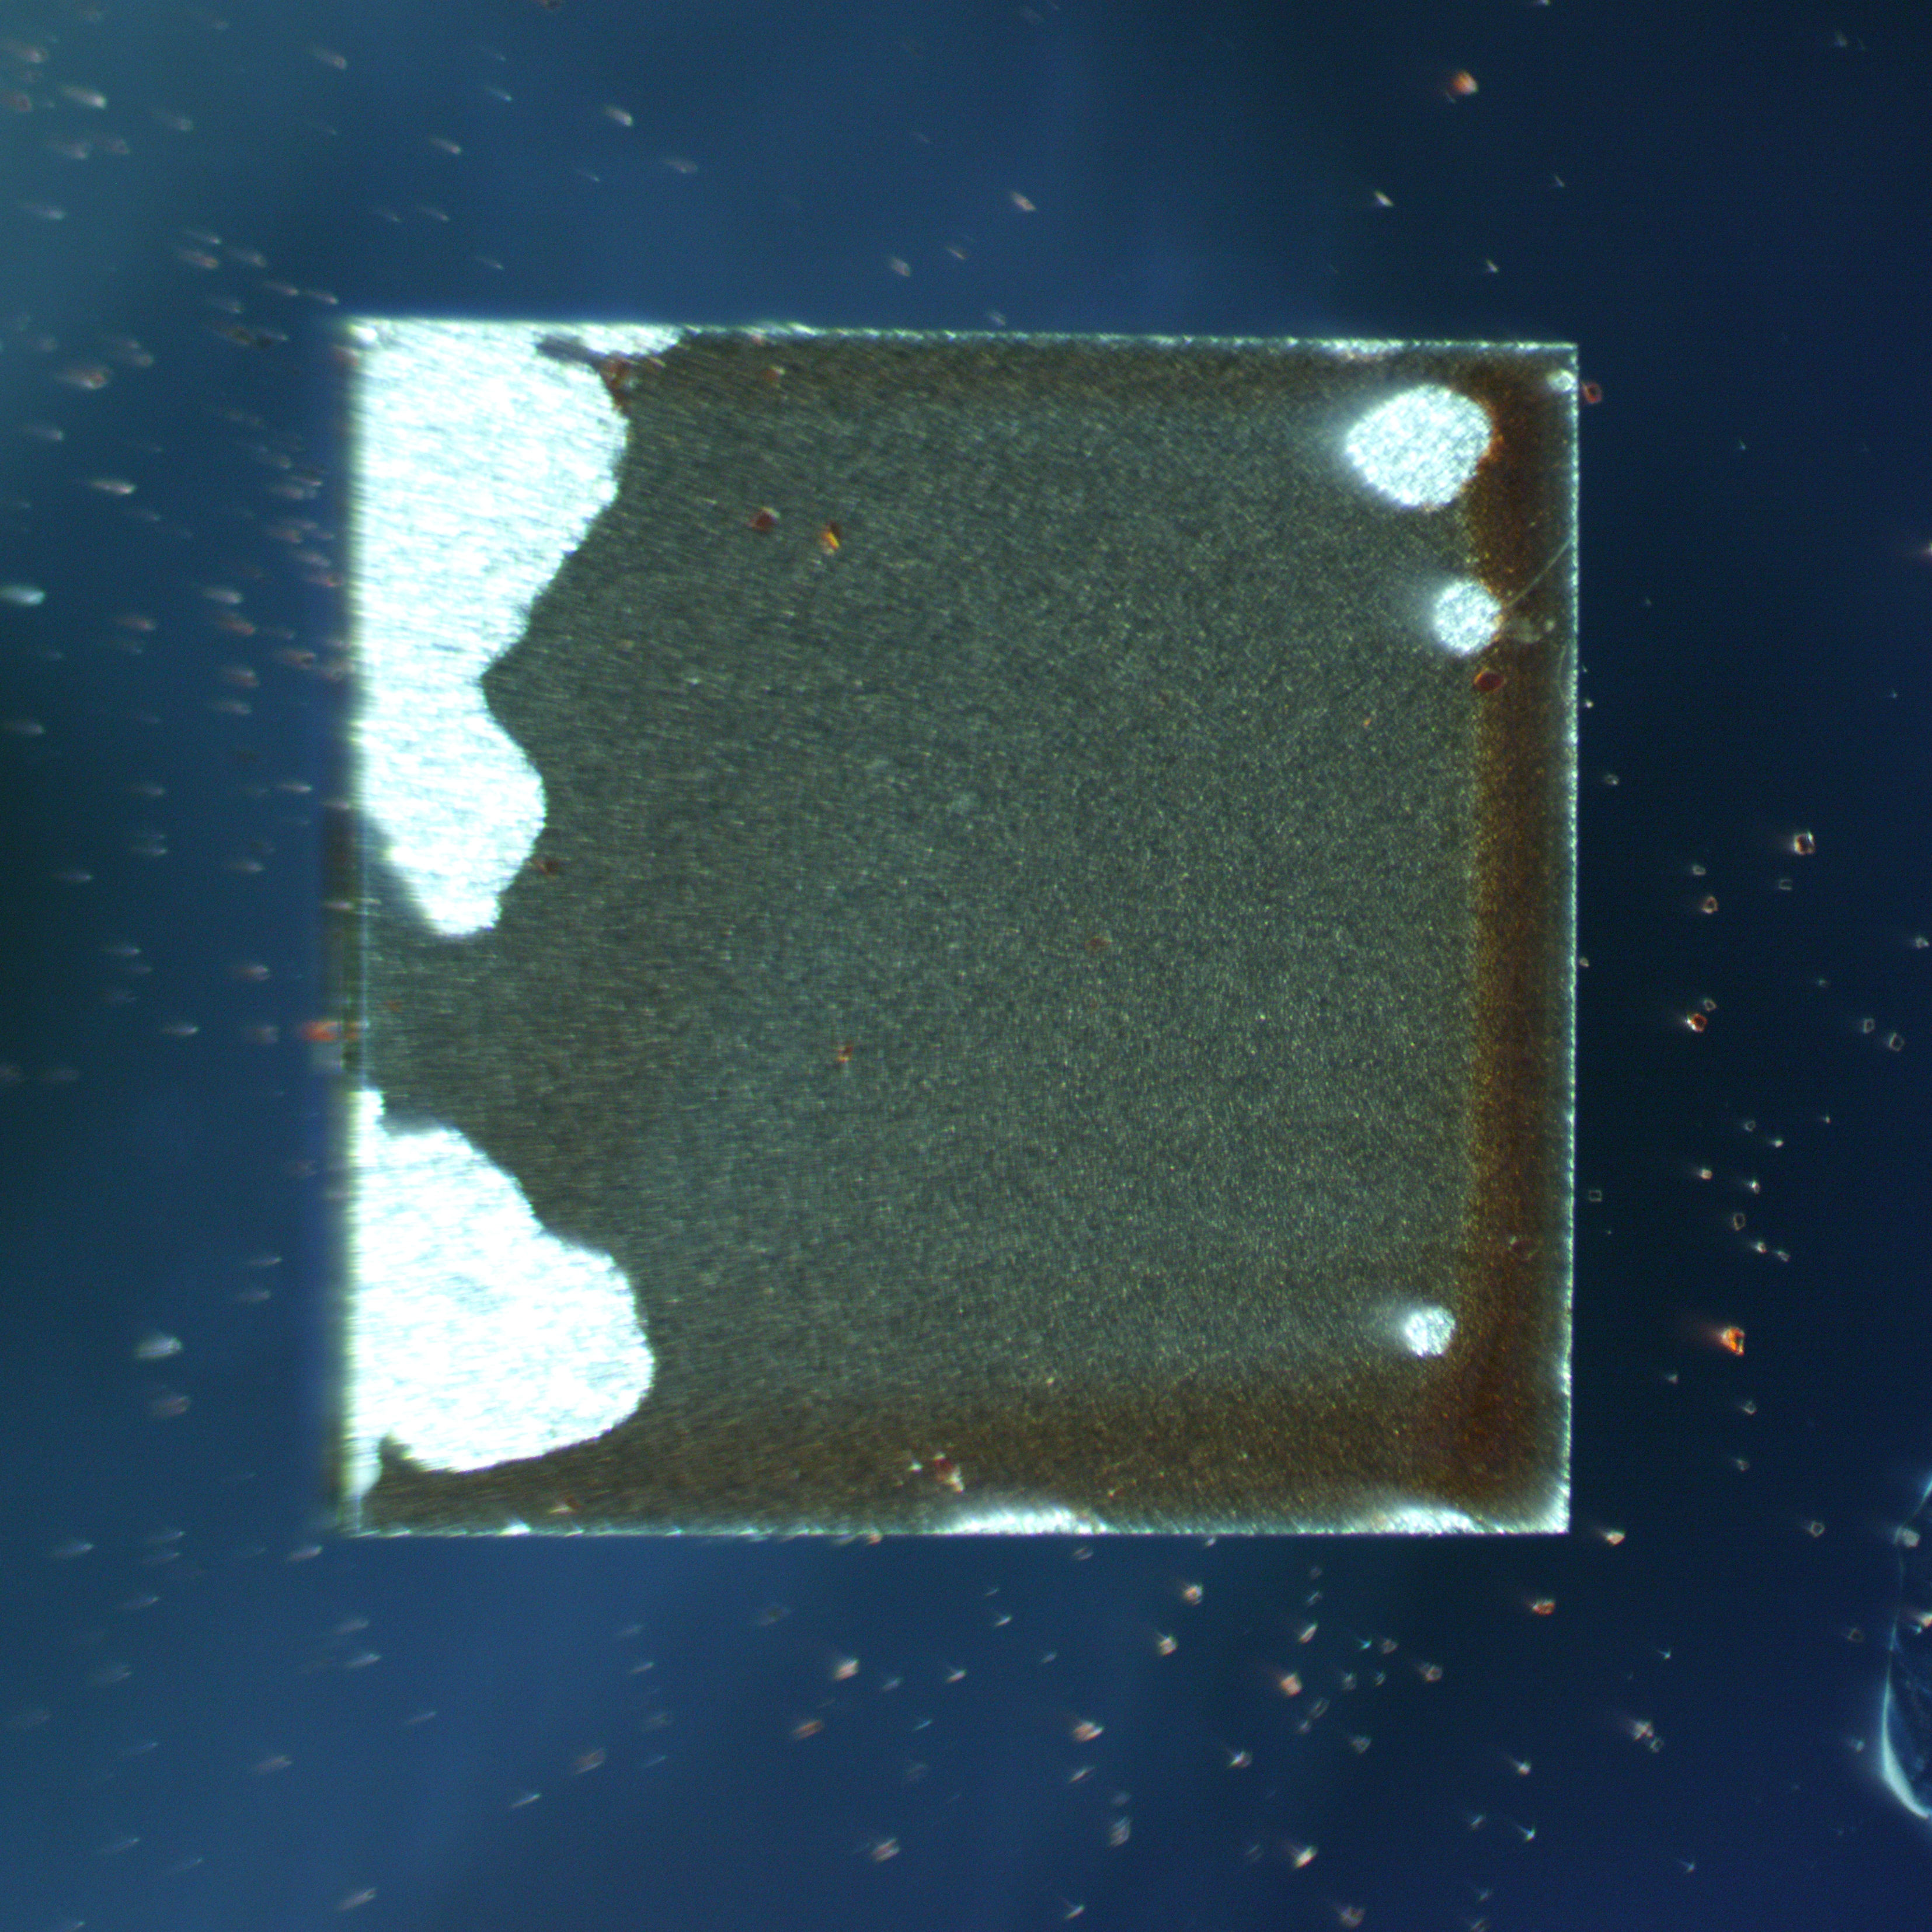
\includegraphics[width=\linewidth]{pics/spincoat/no10/10109.jpg}
        \caption{\textcolor{blue!60!black}{\textbf{Heater 9}}}
    \end{subfigure}

    \caption[Optical Images of the Heater in Passivation Test \#10]{Optical images of the nine Heater of the coating test \#10. The two heaters that could be removed from the glue are highlighted in blue and the height measurement was taken of those marked by a "*"}
    \label{fig:PT10}
\end{figure}
%================================================================================
%================================================================================
\begin{figure}[htbp]
    \centering

    % ---------- Row 1 ----------
    \begin{subfigure}[t]{0.3\textwidth}
        \centering
        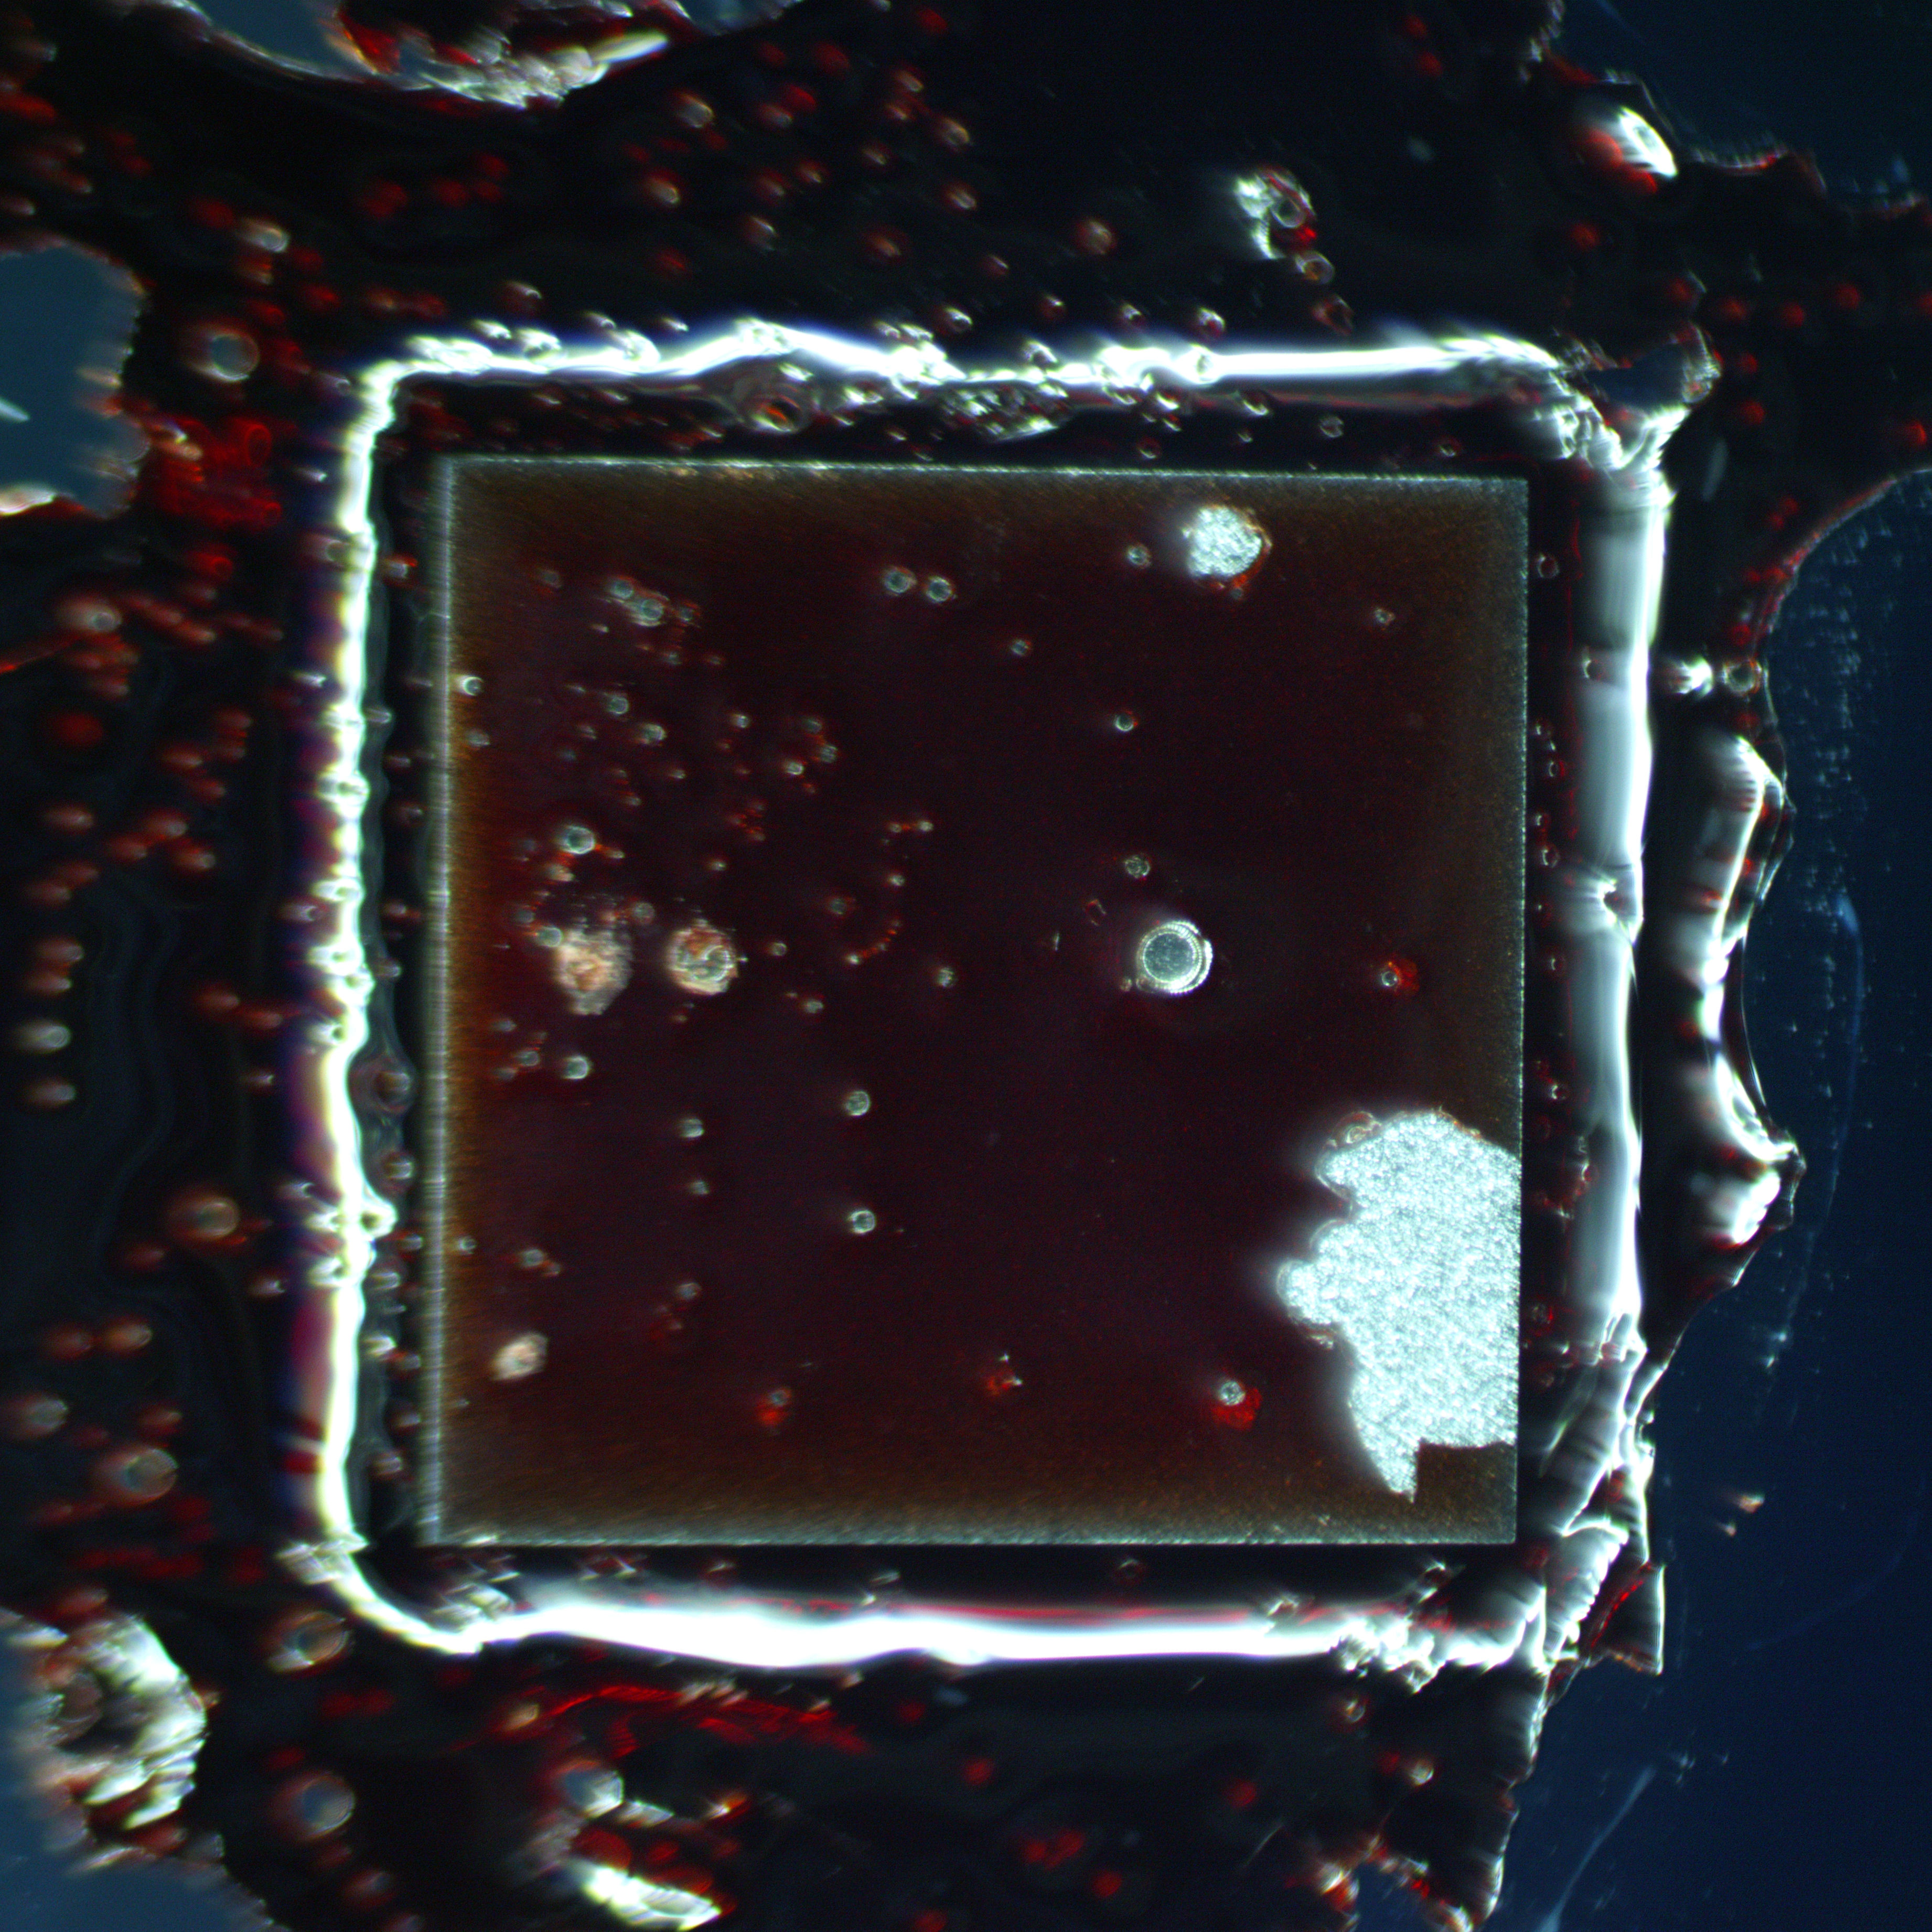
\includegraphics[width=\linewidth]{pics/spincoat/no12/12101.jpg}
        \caption{\textbf{Heater 1*}}
    \end{subfigure}
    \hfill
    \begin{subfigure}[t]{0.3\textwidth}
        \centering
        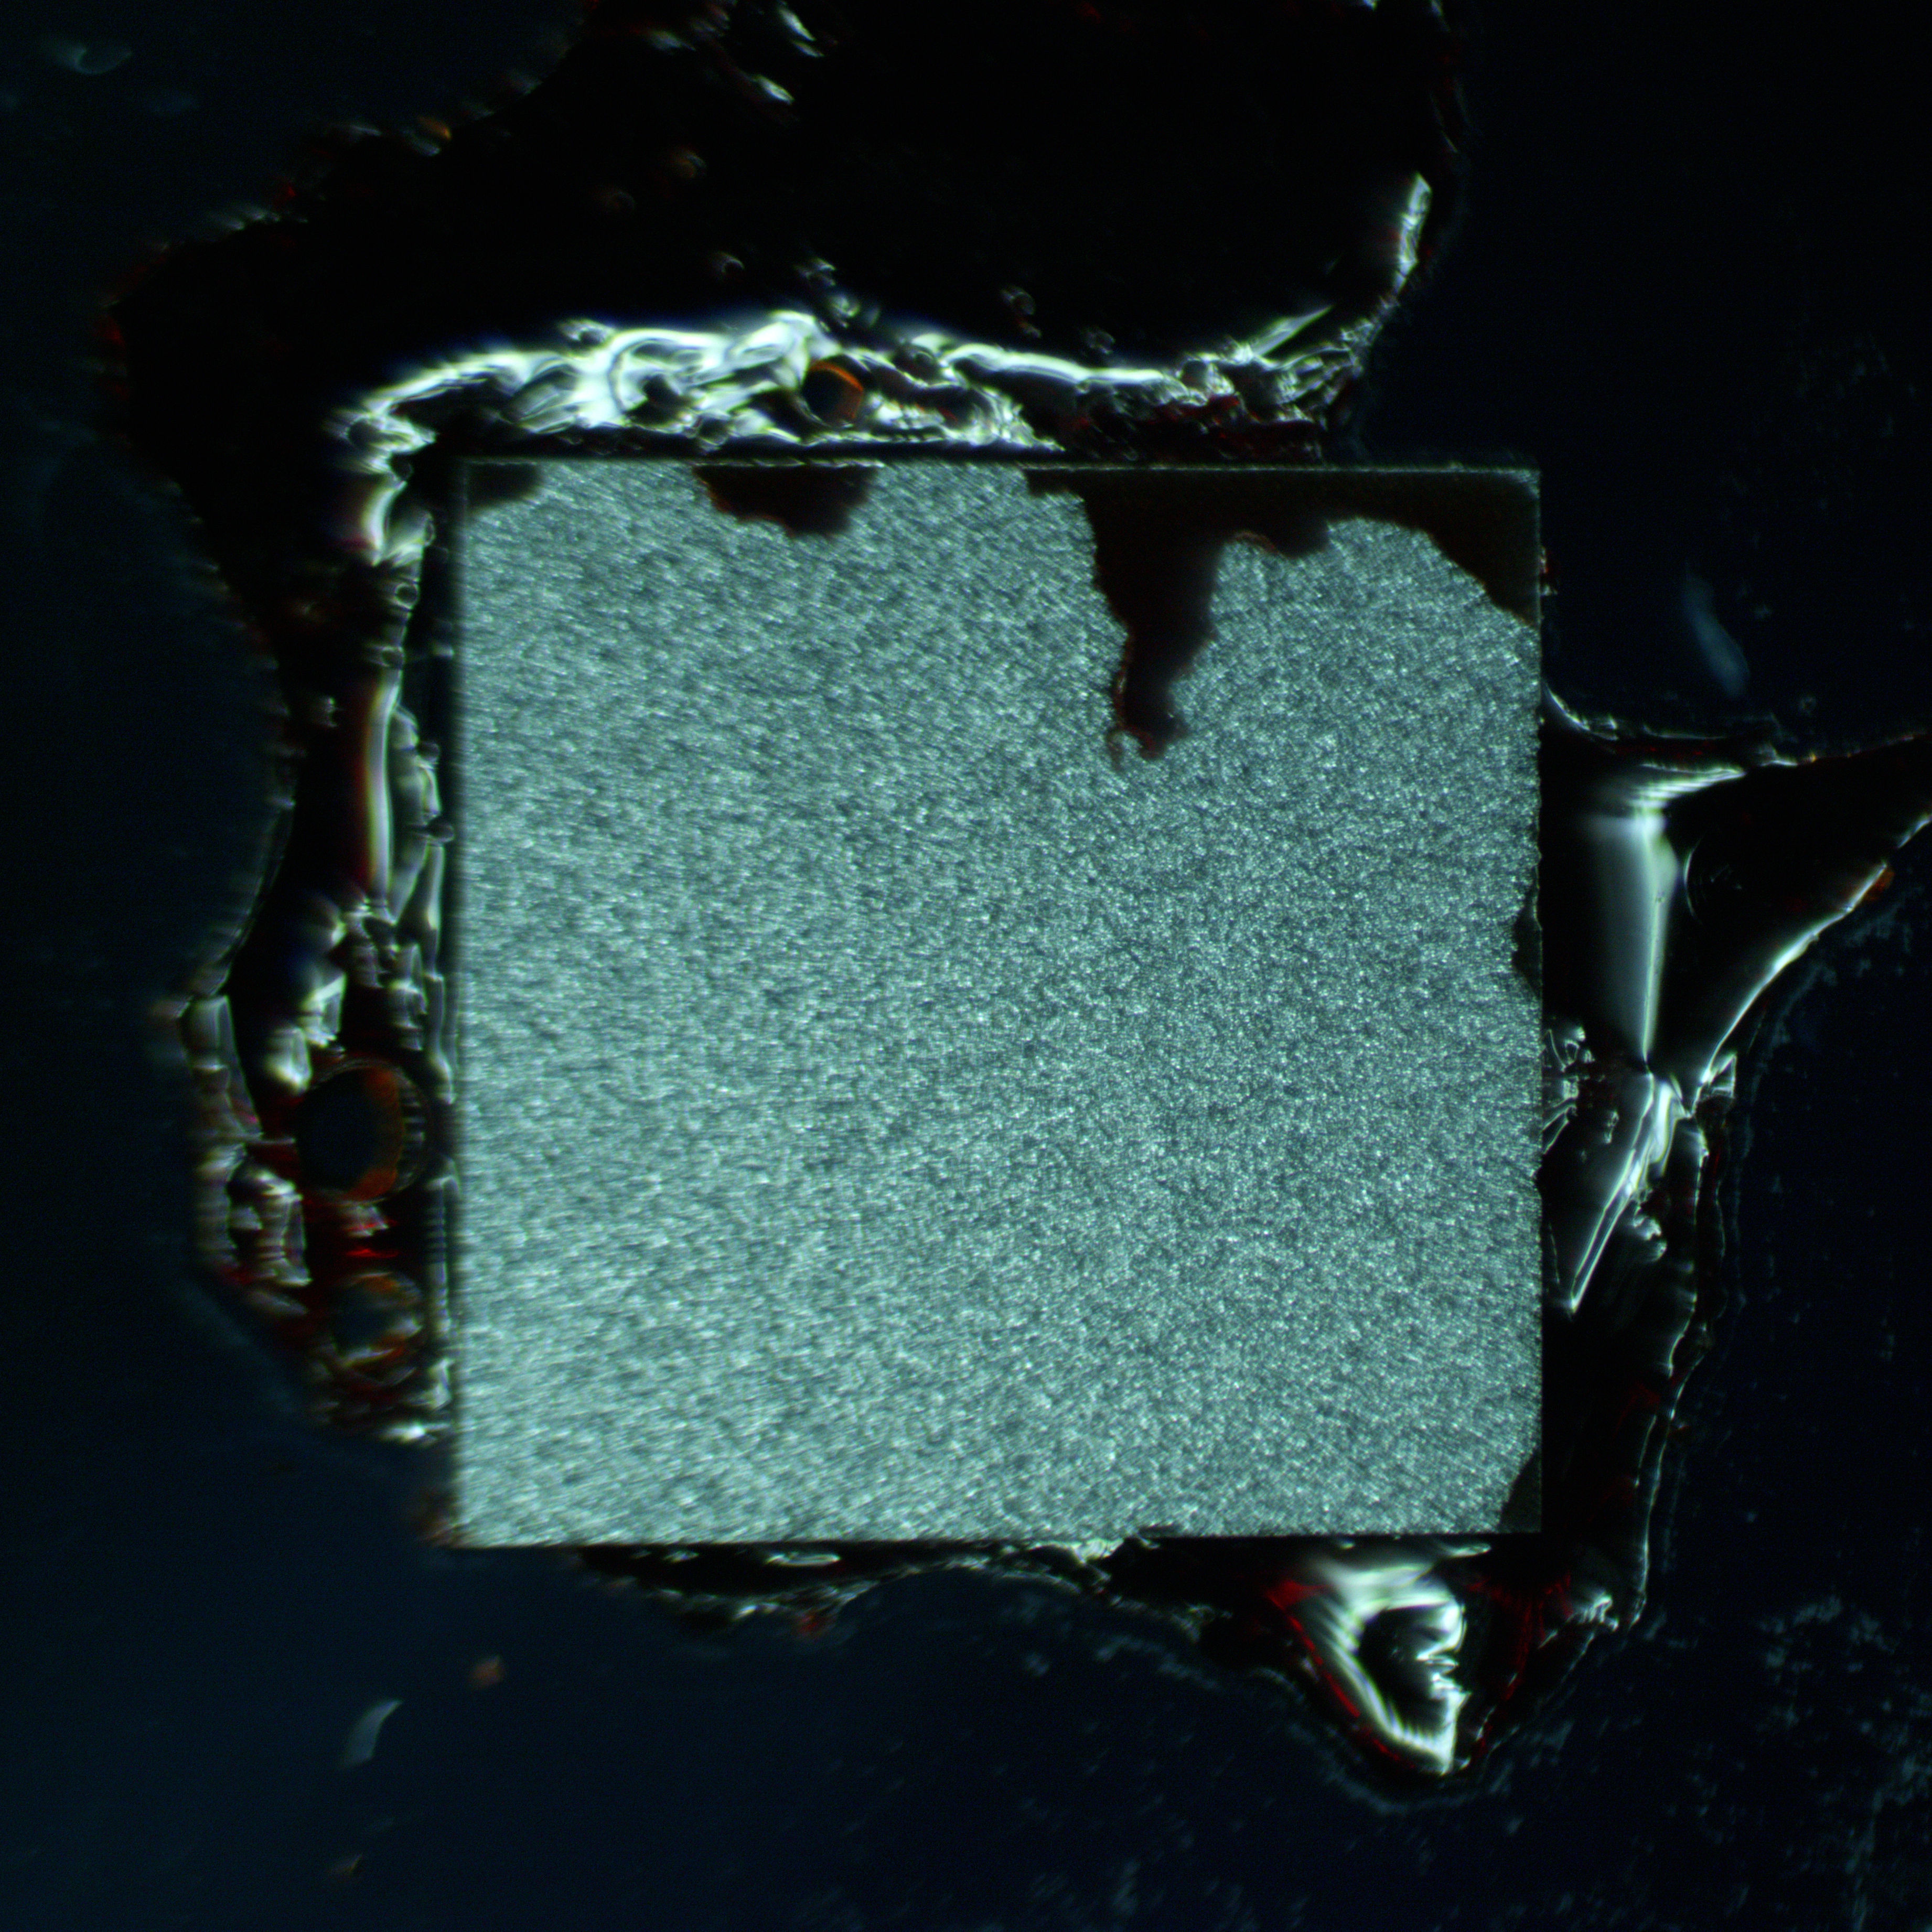
\includegraphics[width=\linewidth]{pics/spincoat/no12/12102.jpg}
        \caption{Heater 2}
    \end{subfigure}
    \hfill
    \begin{subfigure}[t]{0.3\textwidth}
        \centering
        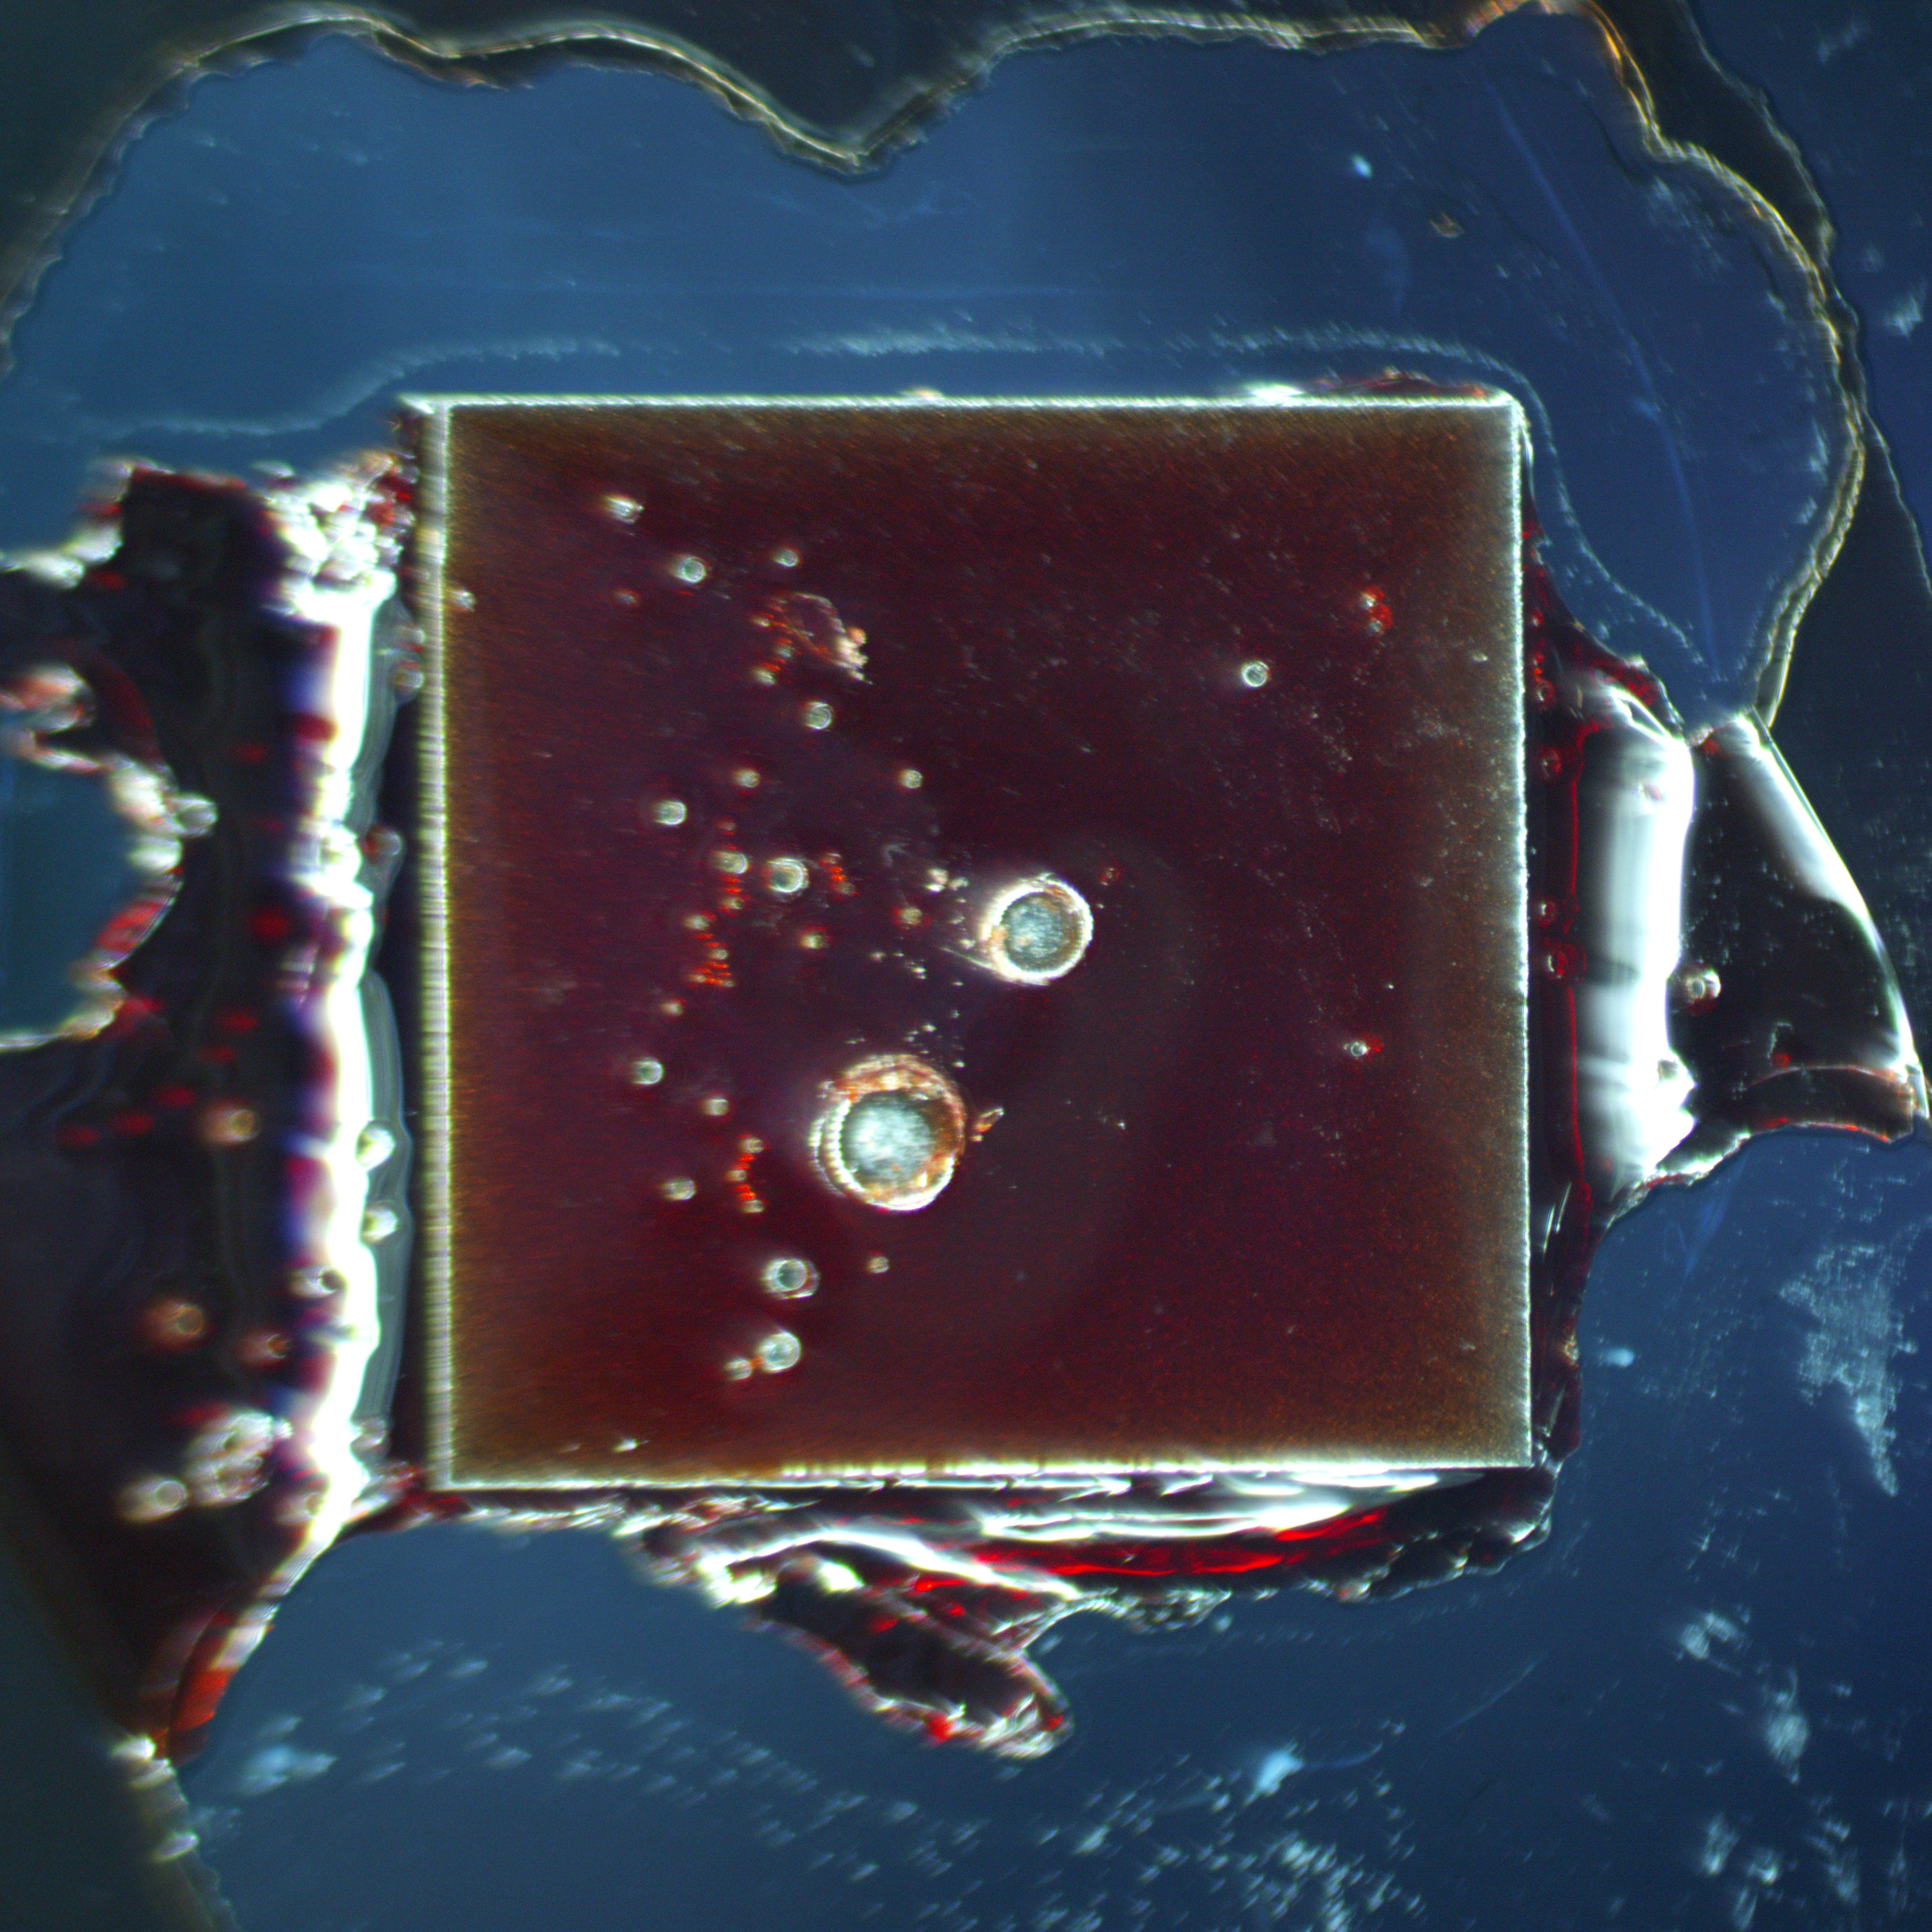
\includegraphics[width=\linewidth]{pics/spincoat/no12/12103.jpg}
        \caption{Heater 3}
    \end{subfigure}

    \vspace{0.8cm}

    % ---------- Row 2 ----------
    \begin{subfigure}[t]{0.3\textwidth}
        \centering
        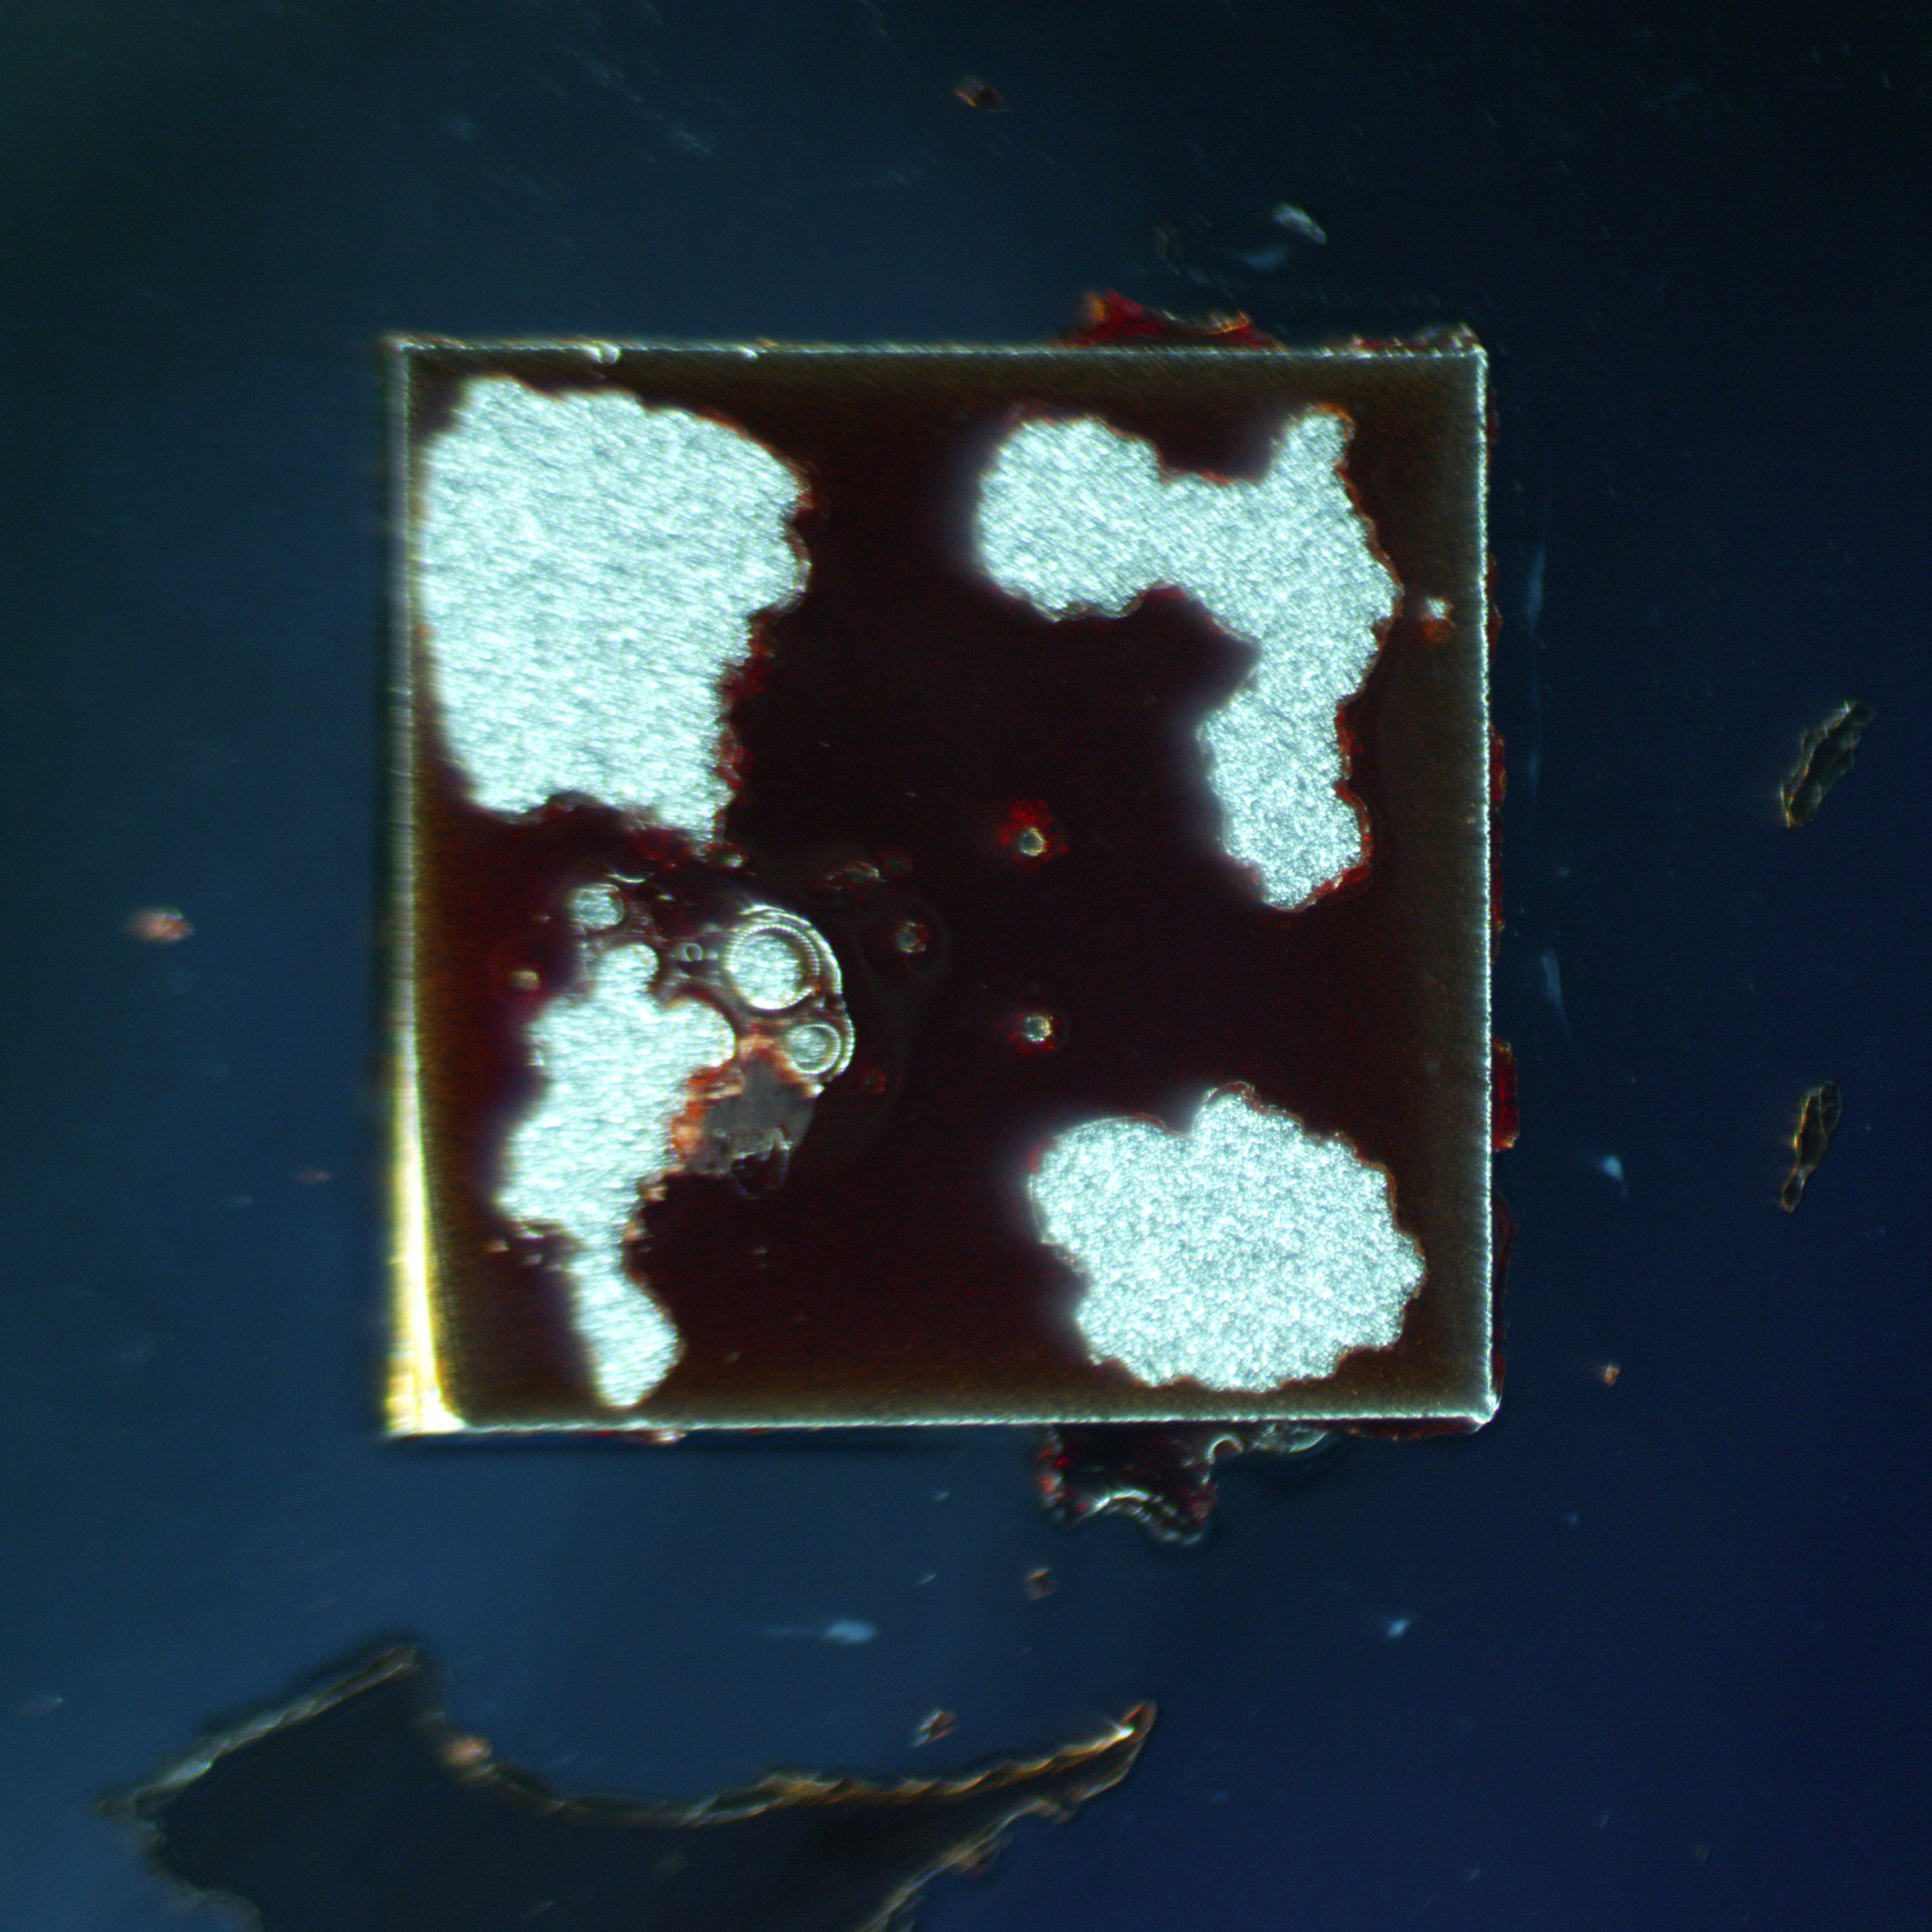
\includegraphics[width=\linewidth]{pics/spincoat/no12/12104.jpg}
        \caption{Heater 4}
    \end{subfigure}
    \hfill
    \begin{subfigure}[t]{0.3\textwidth}
        \centering
        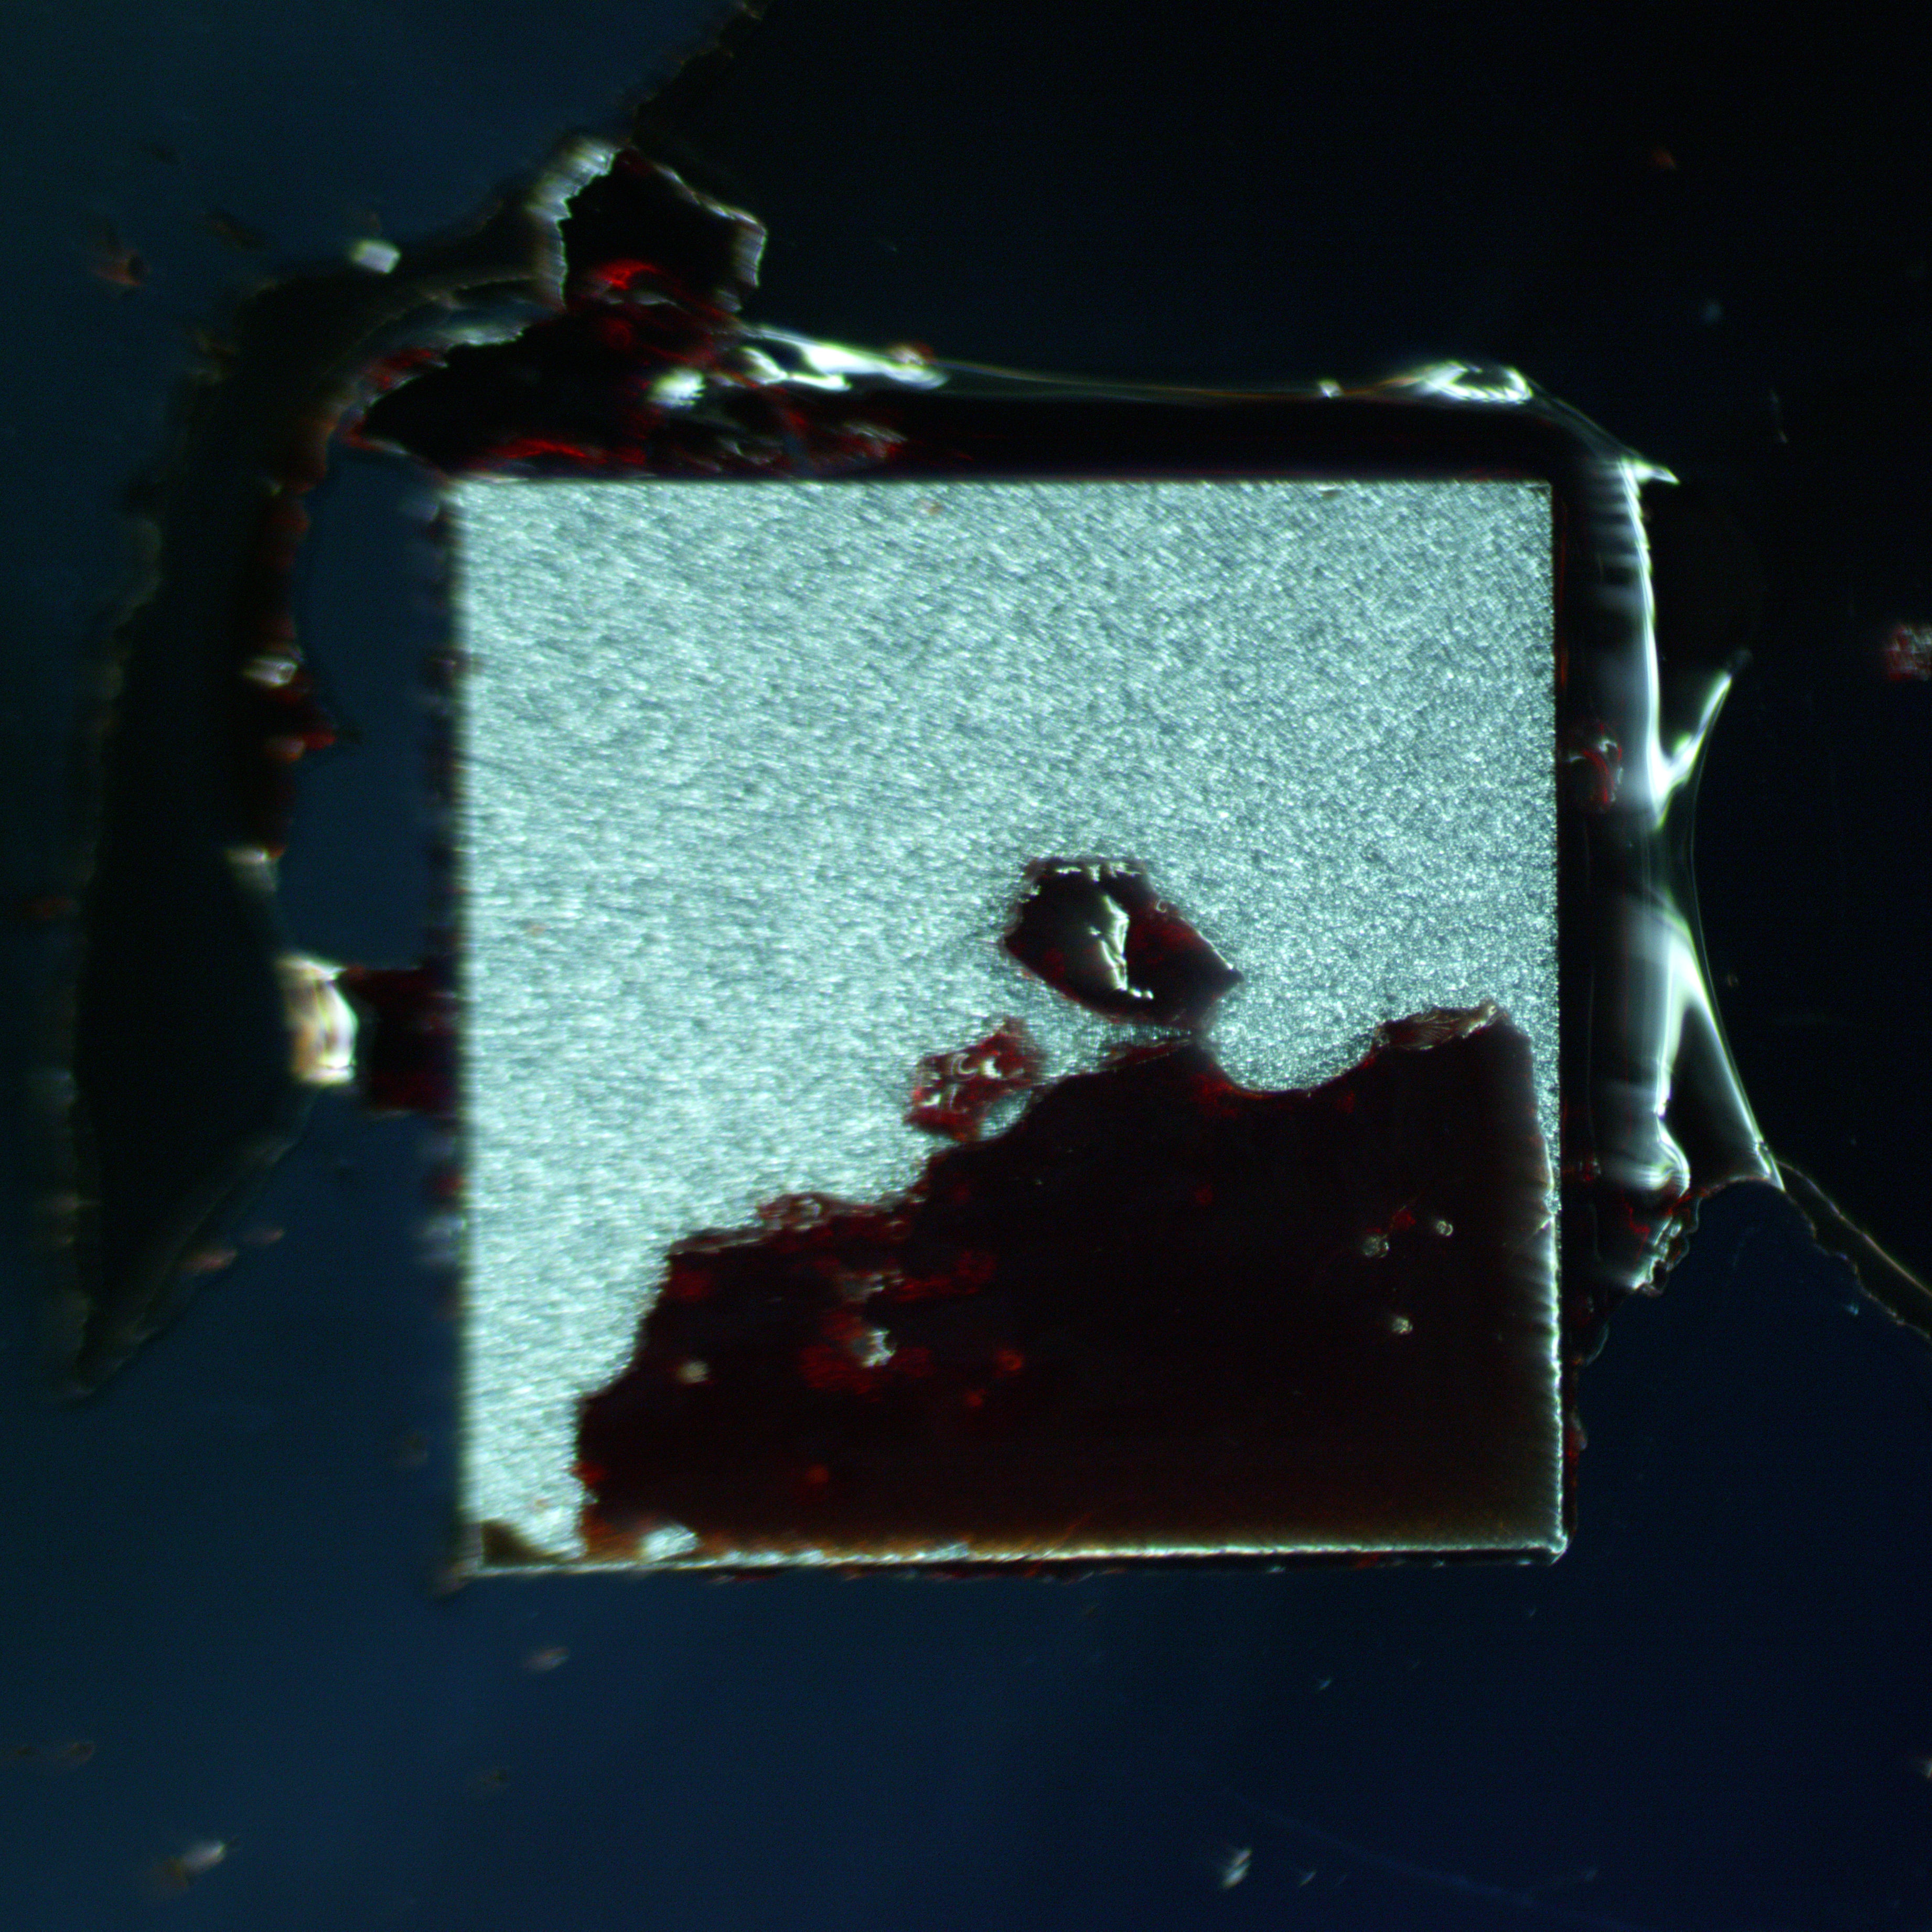
\includegraphics[width=\linewidth]{pics/spincoat/no12/12105.jpg}
        \caption{Heater 5}
    \end{subfigure}
    \hfill
    \begin{subfigure}[t]{0.3\textwidth}
        \centering
        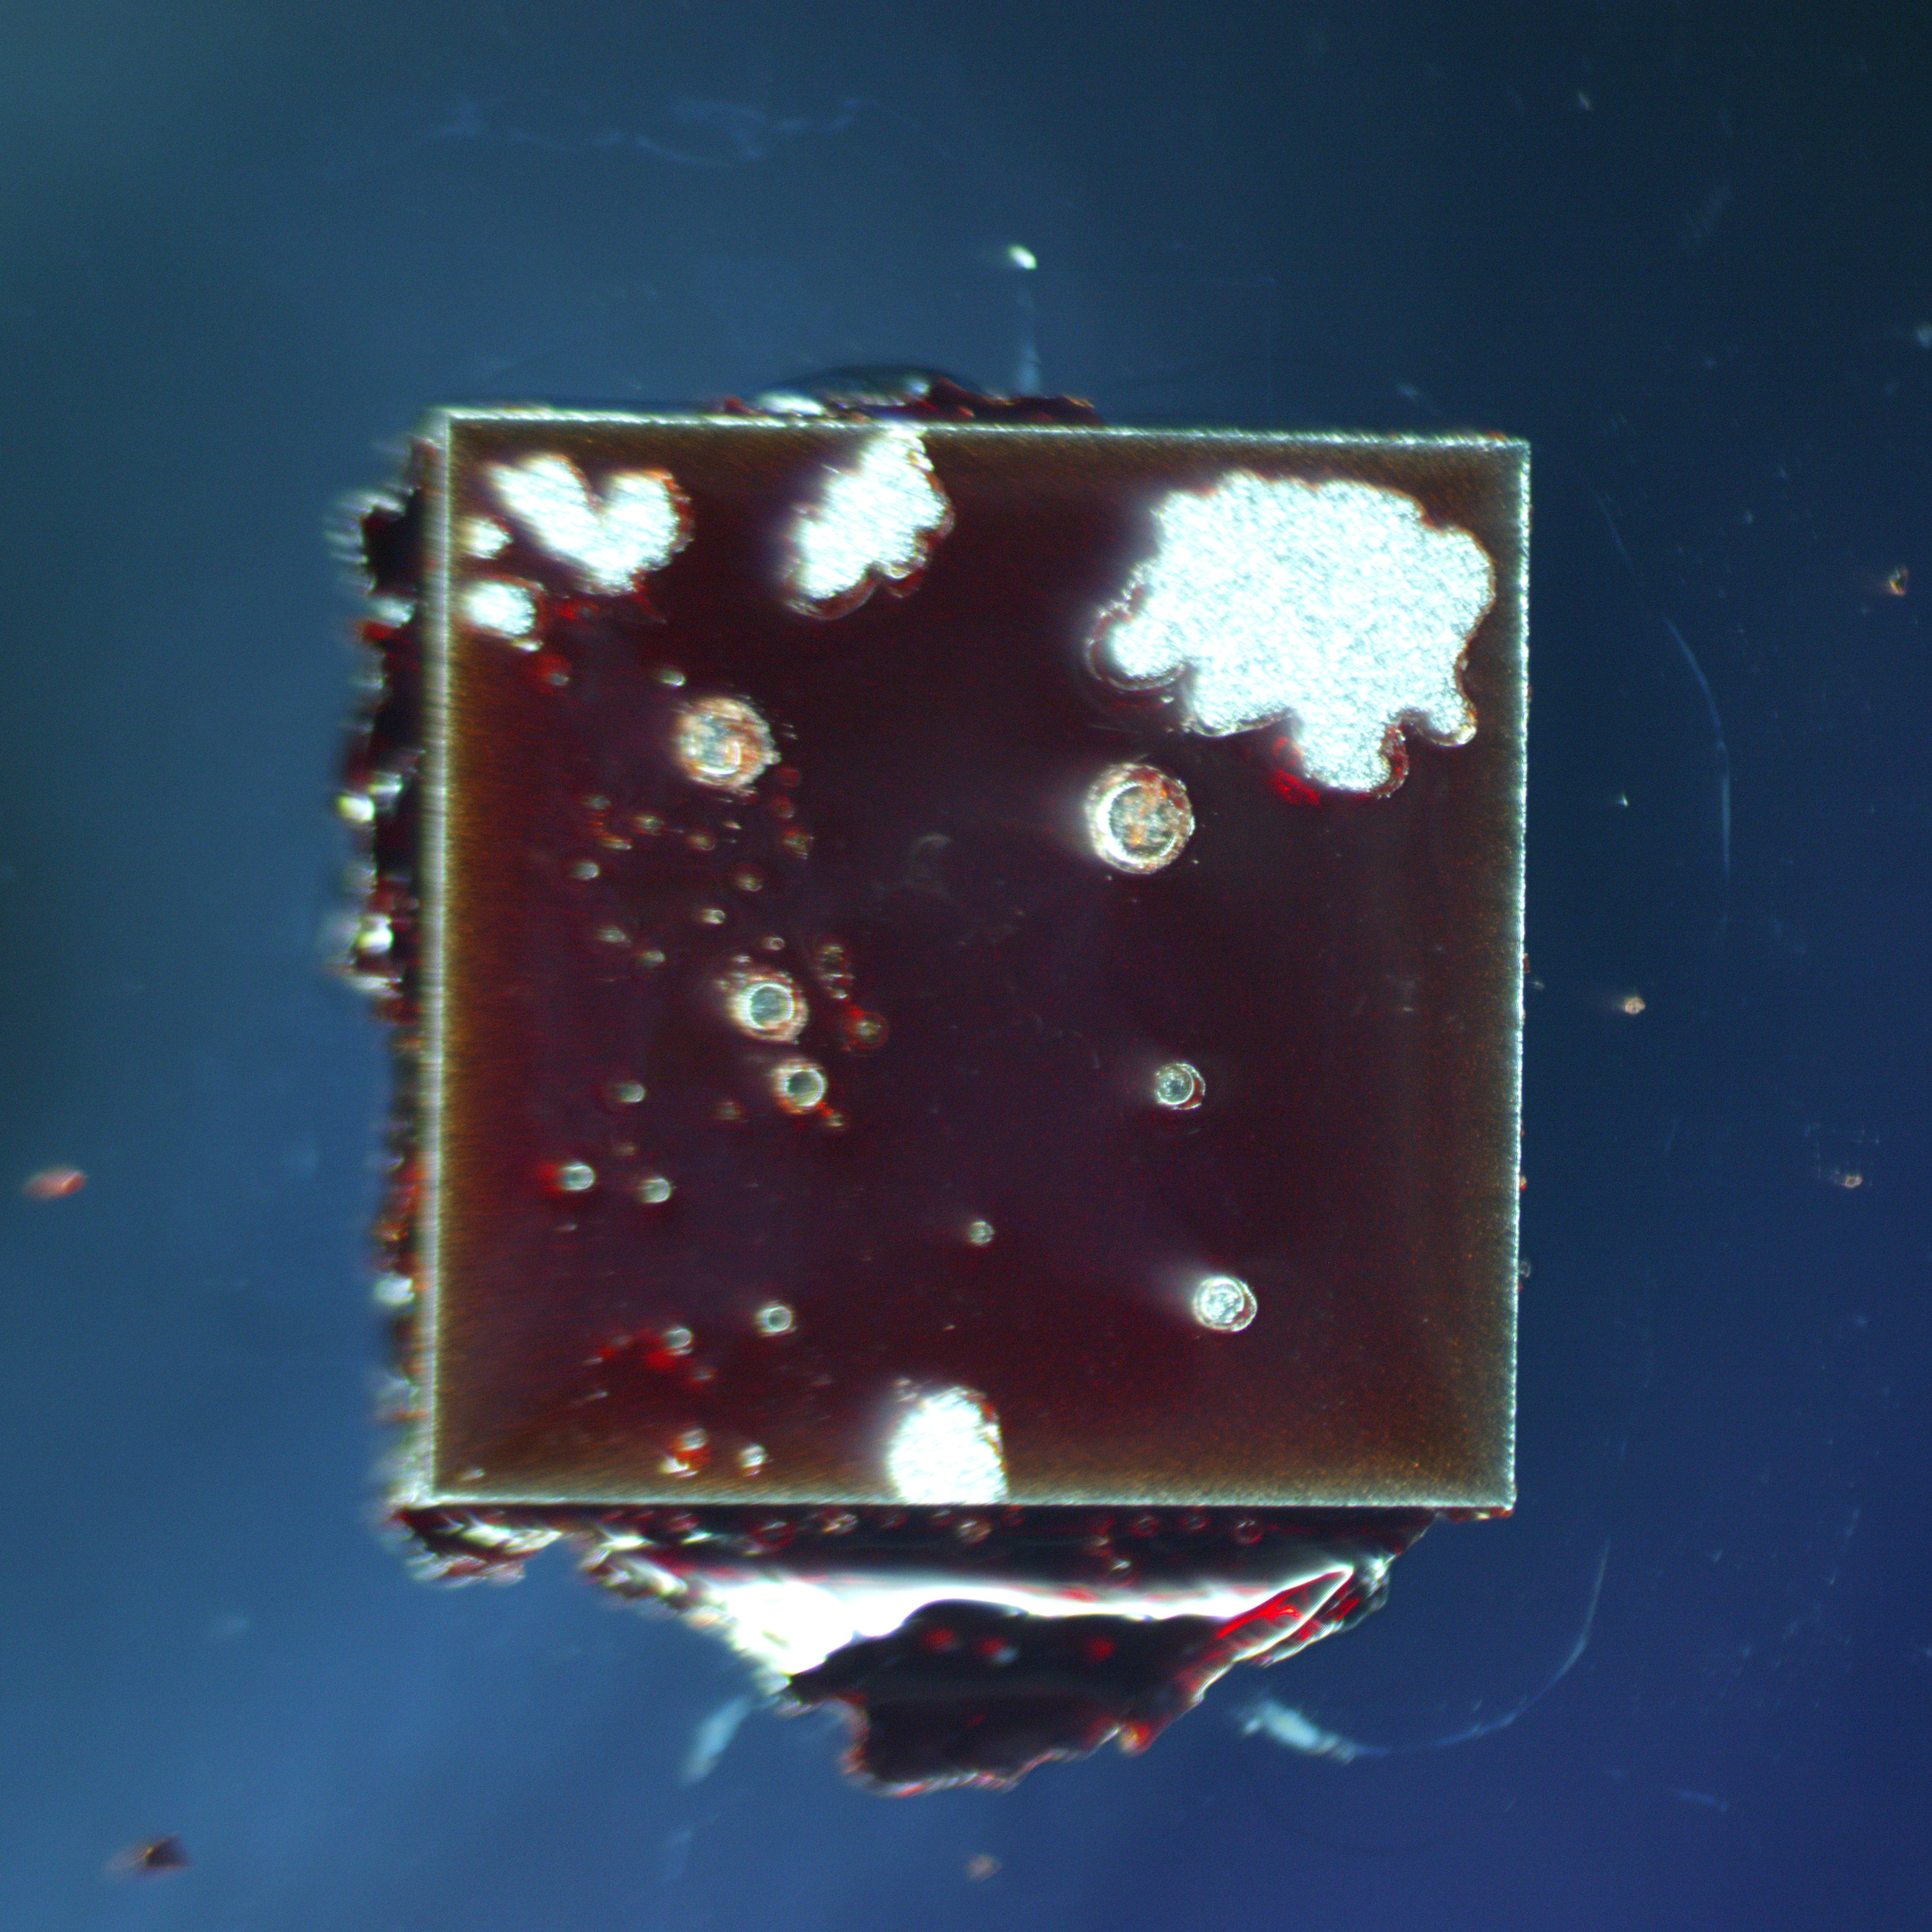
\includegraphics[width=\linewidth]{pics/spincoat/no12/12106.jpg}
        \caption{Heater 6}
    \end{subfigure}

    \vspace{0.8cm}

    % ---------- Row 3 ----------
    \begin{subfigure}[t]{0.3\textwidth}
        \centering
        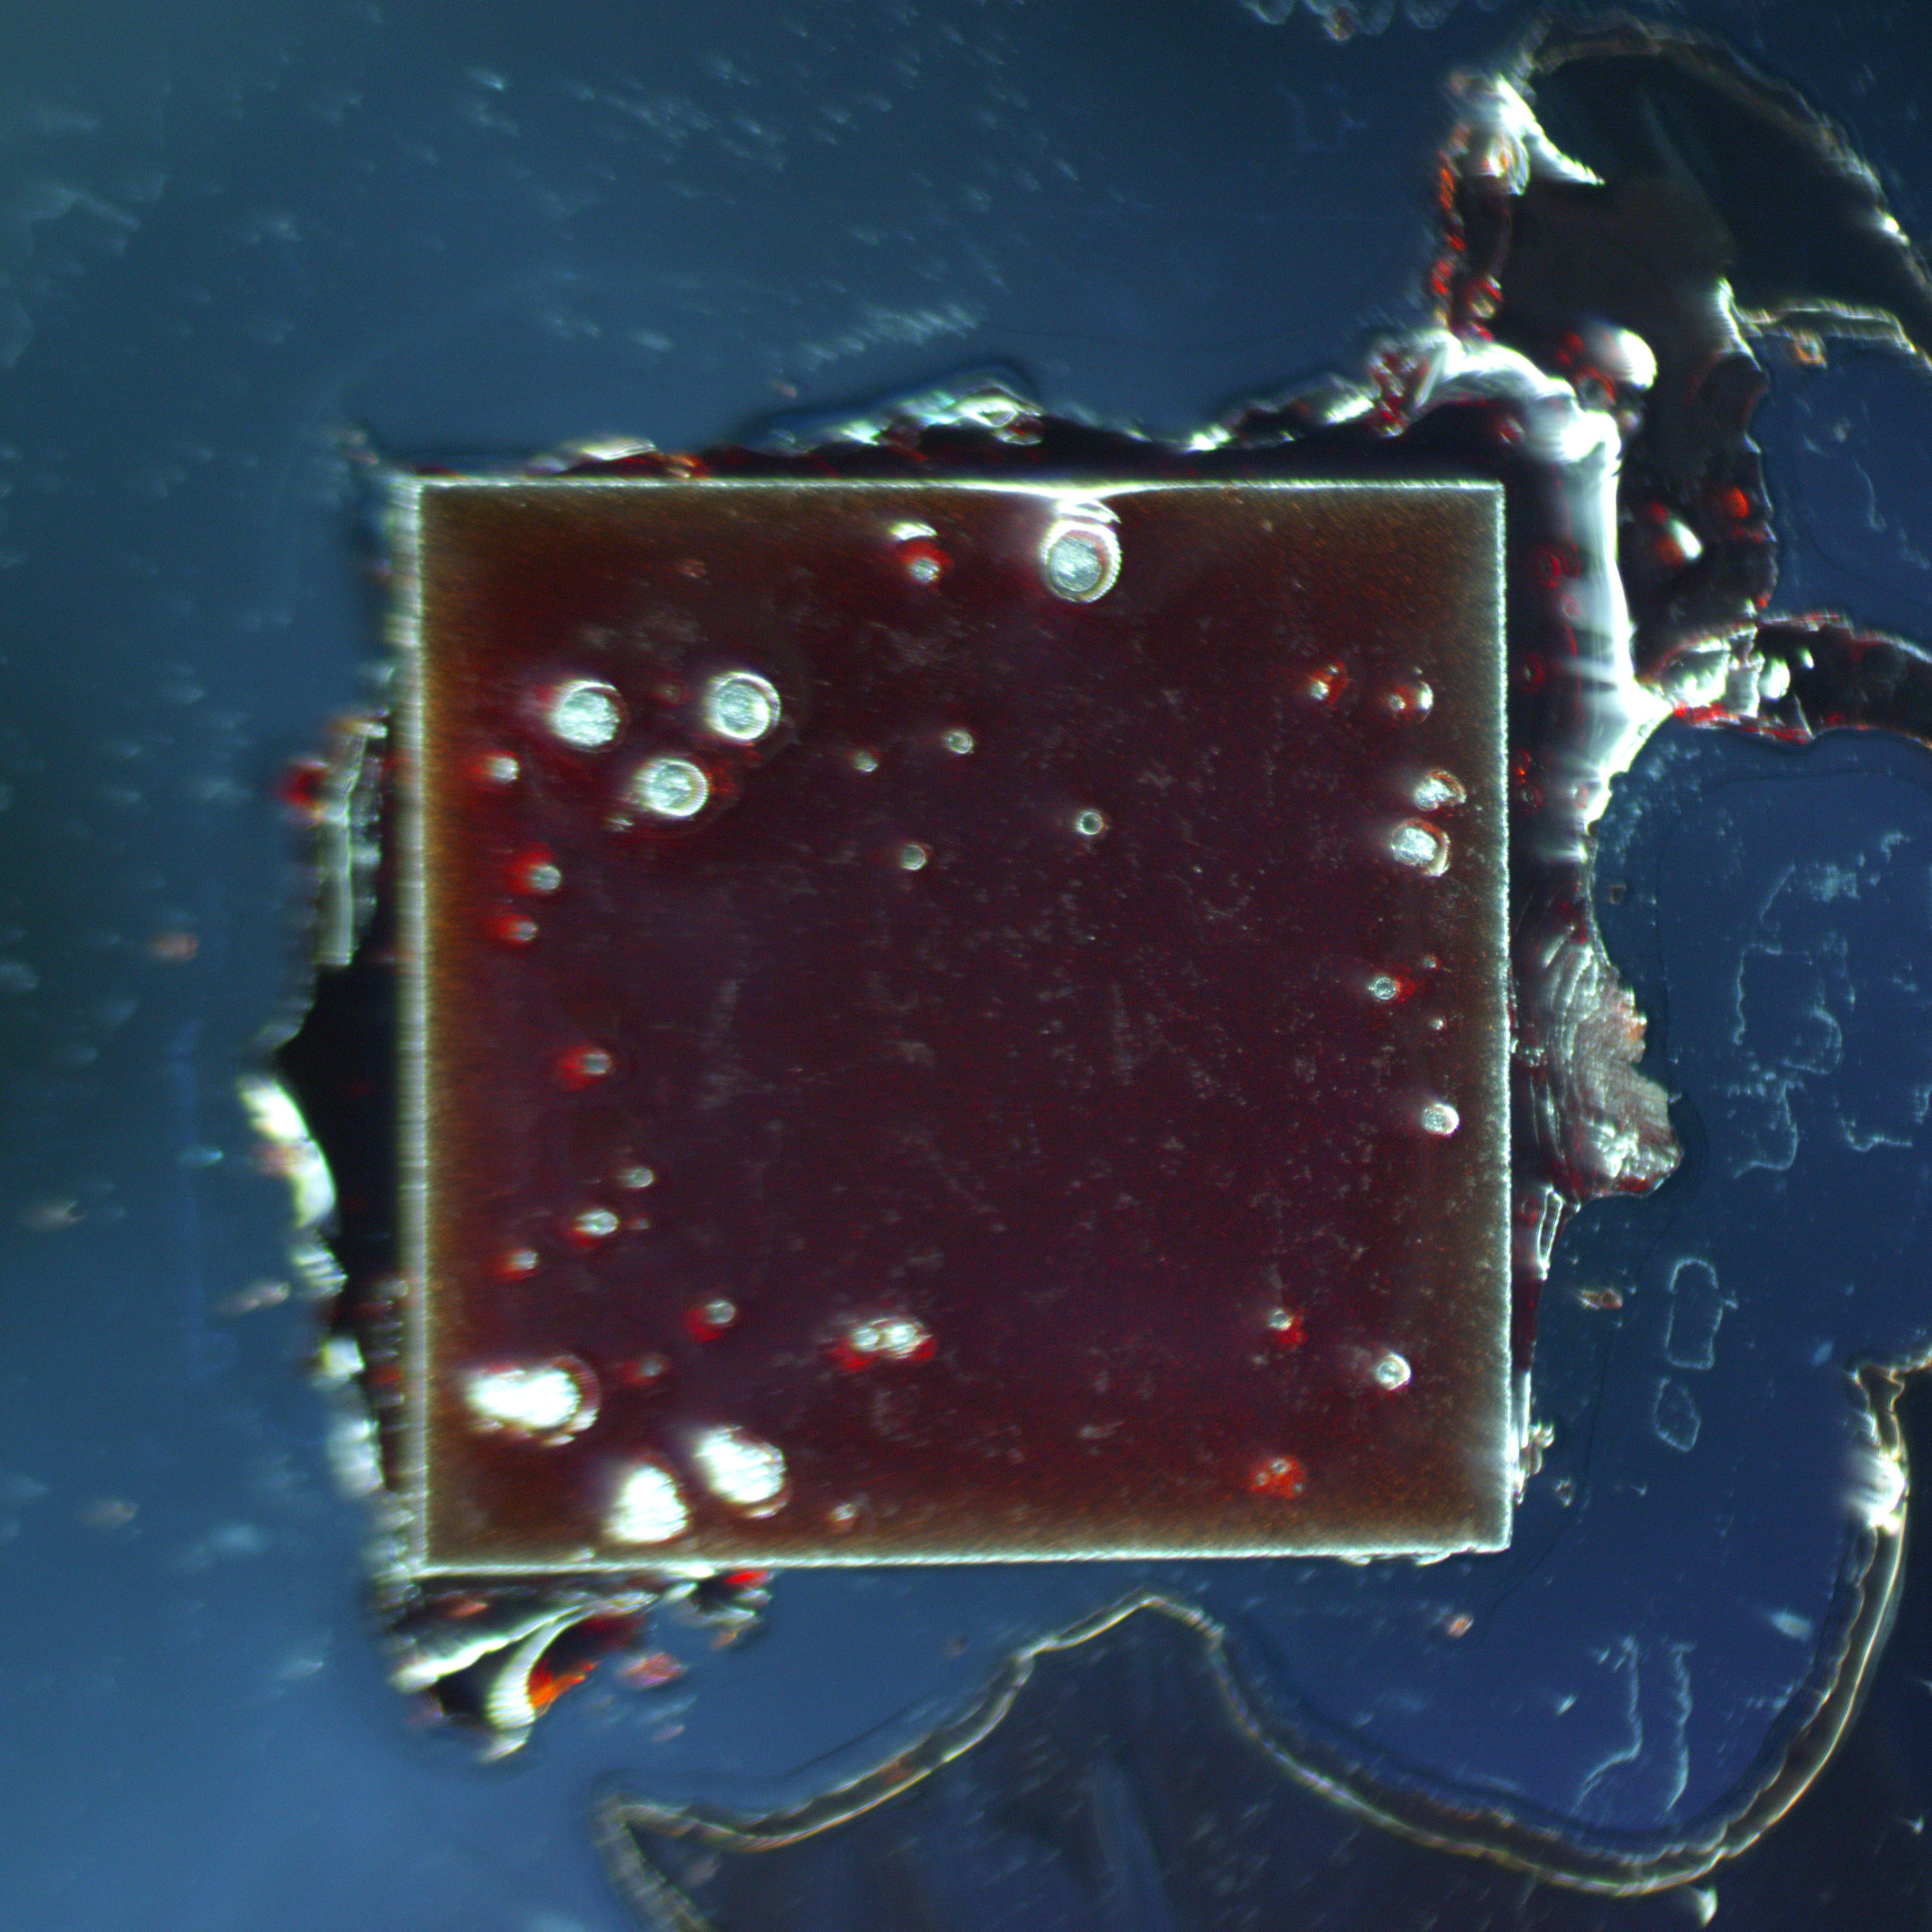
\includegraphics[width=\linewidth]{pics/spincoat/no12/12107.jpg}
        \caption{Heater 7}
    \end{subfigure}
    \hfill
    \begin{subfigure}[t]{0.3\textwidth}
        \centering
        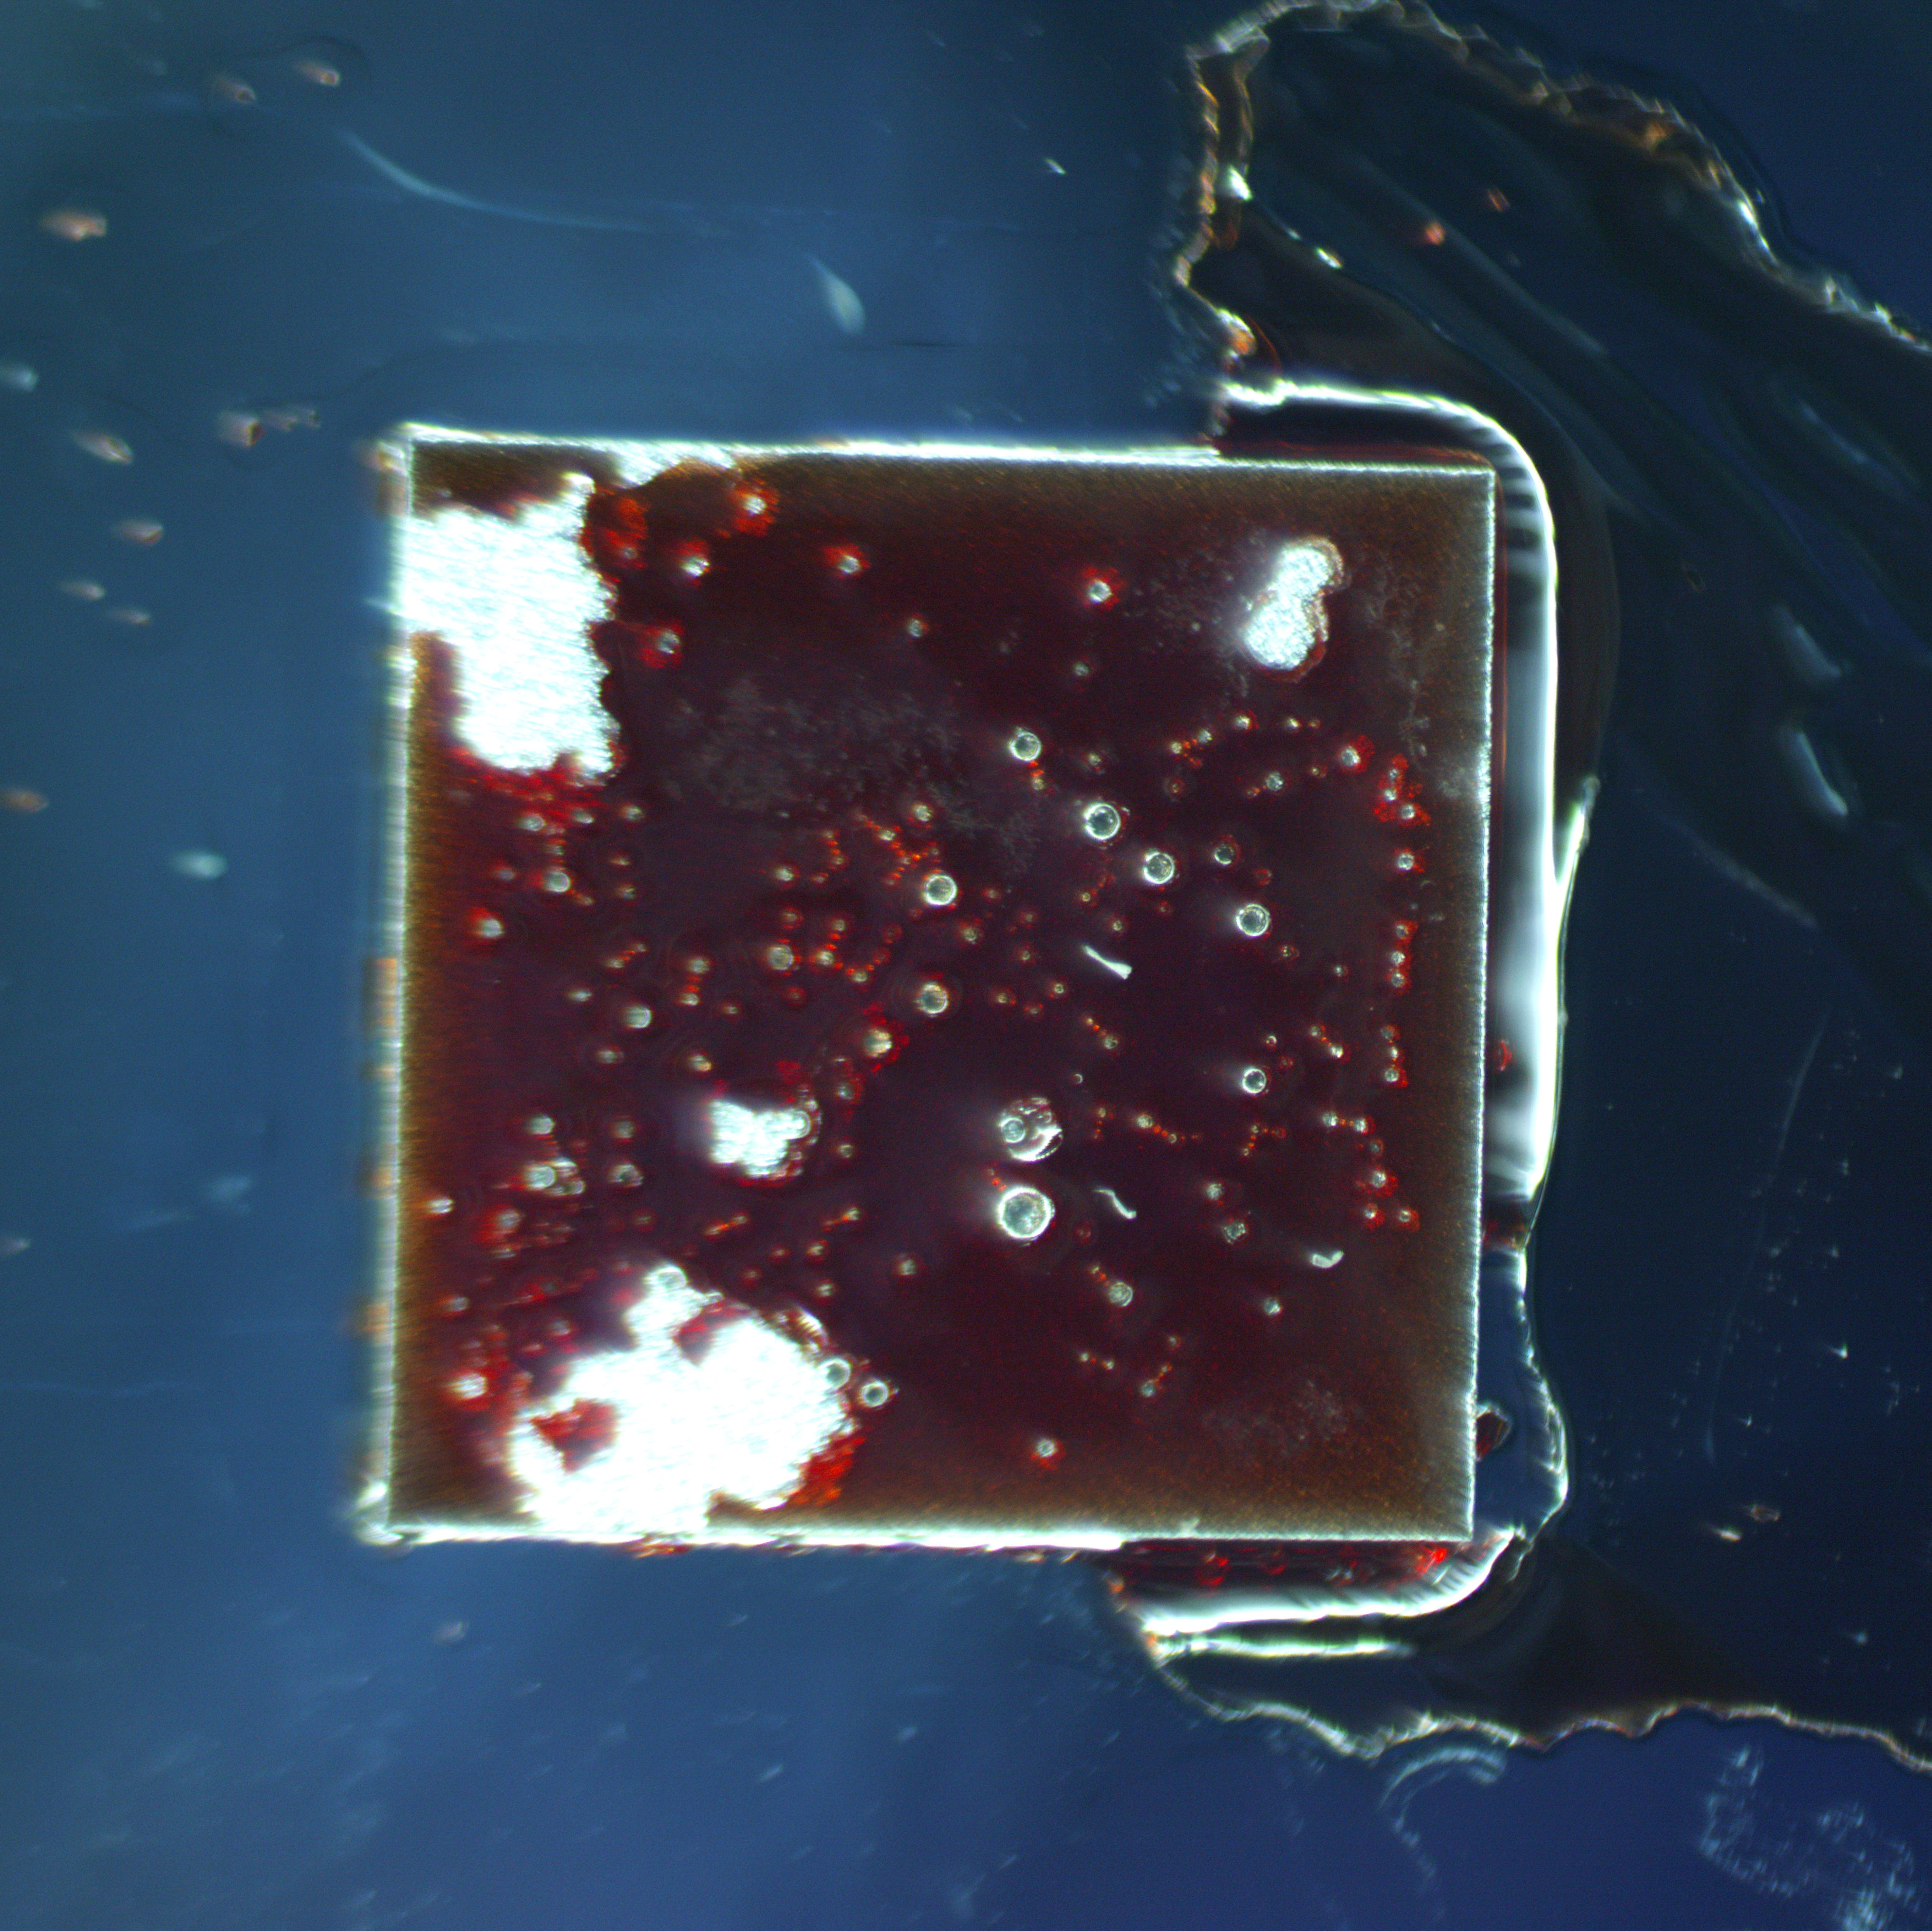
\includegraphics[width=\linewidth]{pics/spincoat/no12/12108.jpg}
        \caption{Heater 8}
    \end{subfigure}
    \hfill
    \begin{subfigure}[t]{0.3\textwidth}
        \centering
        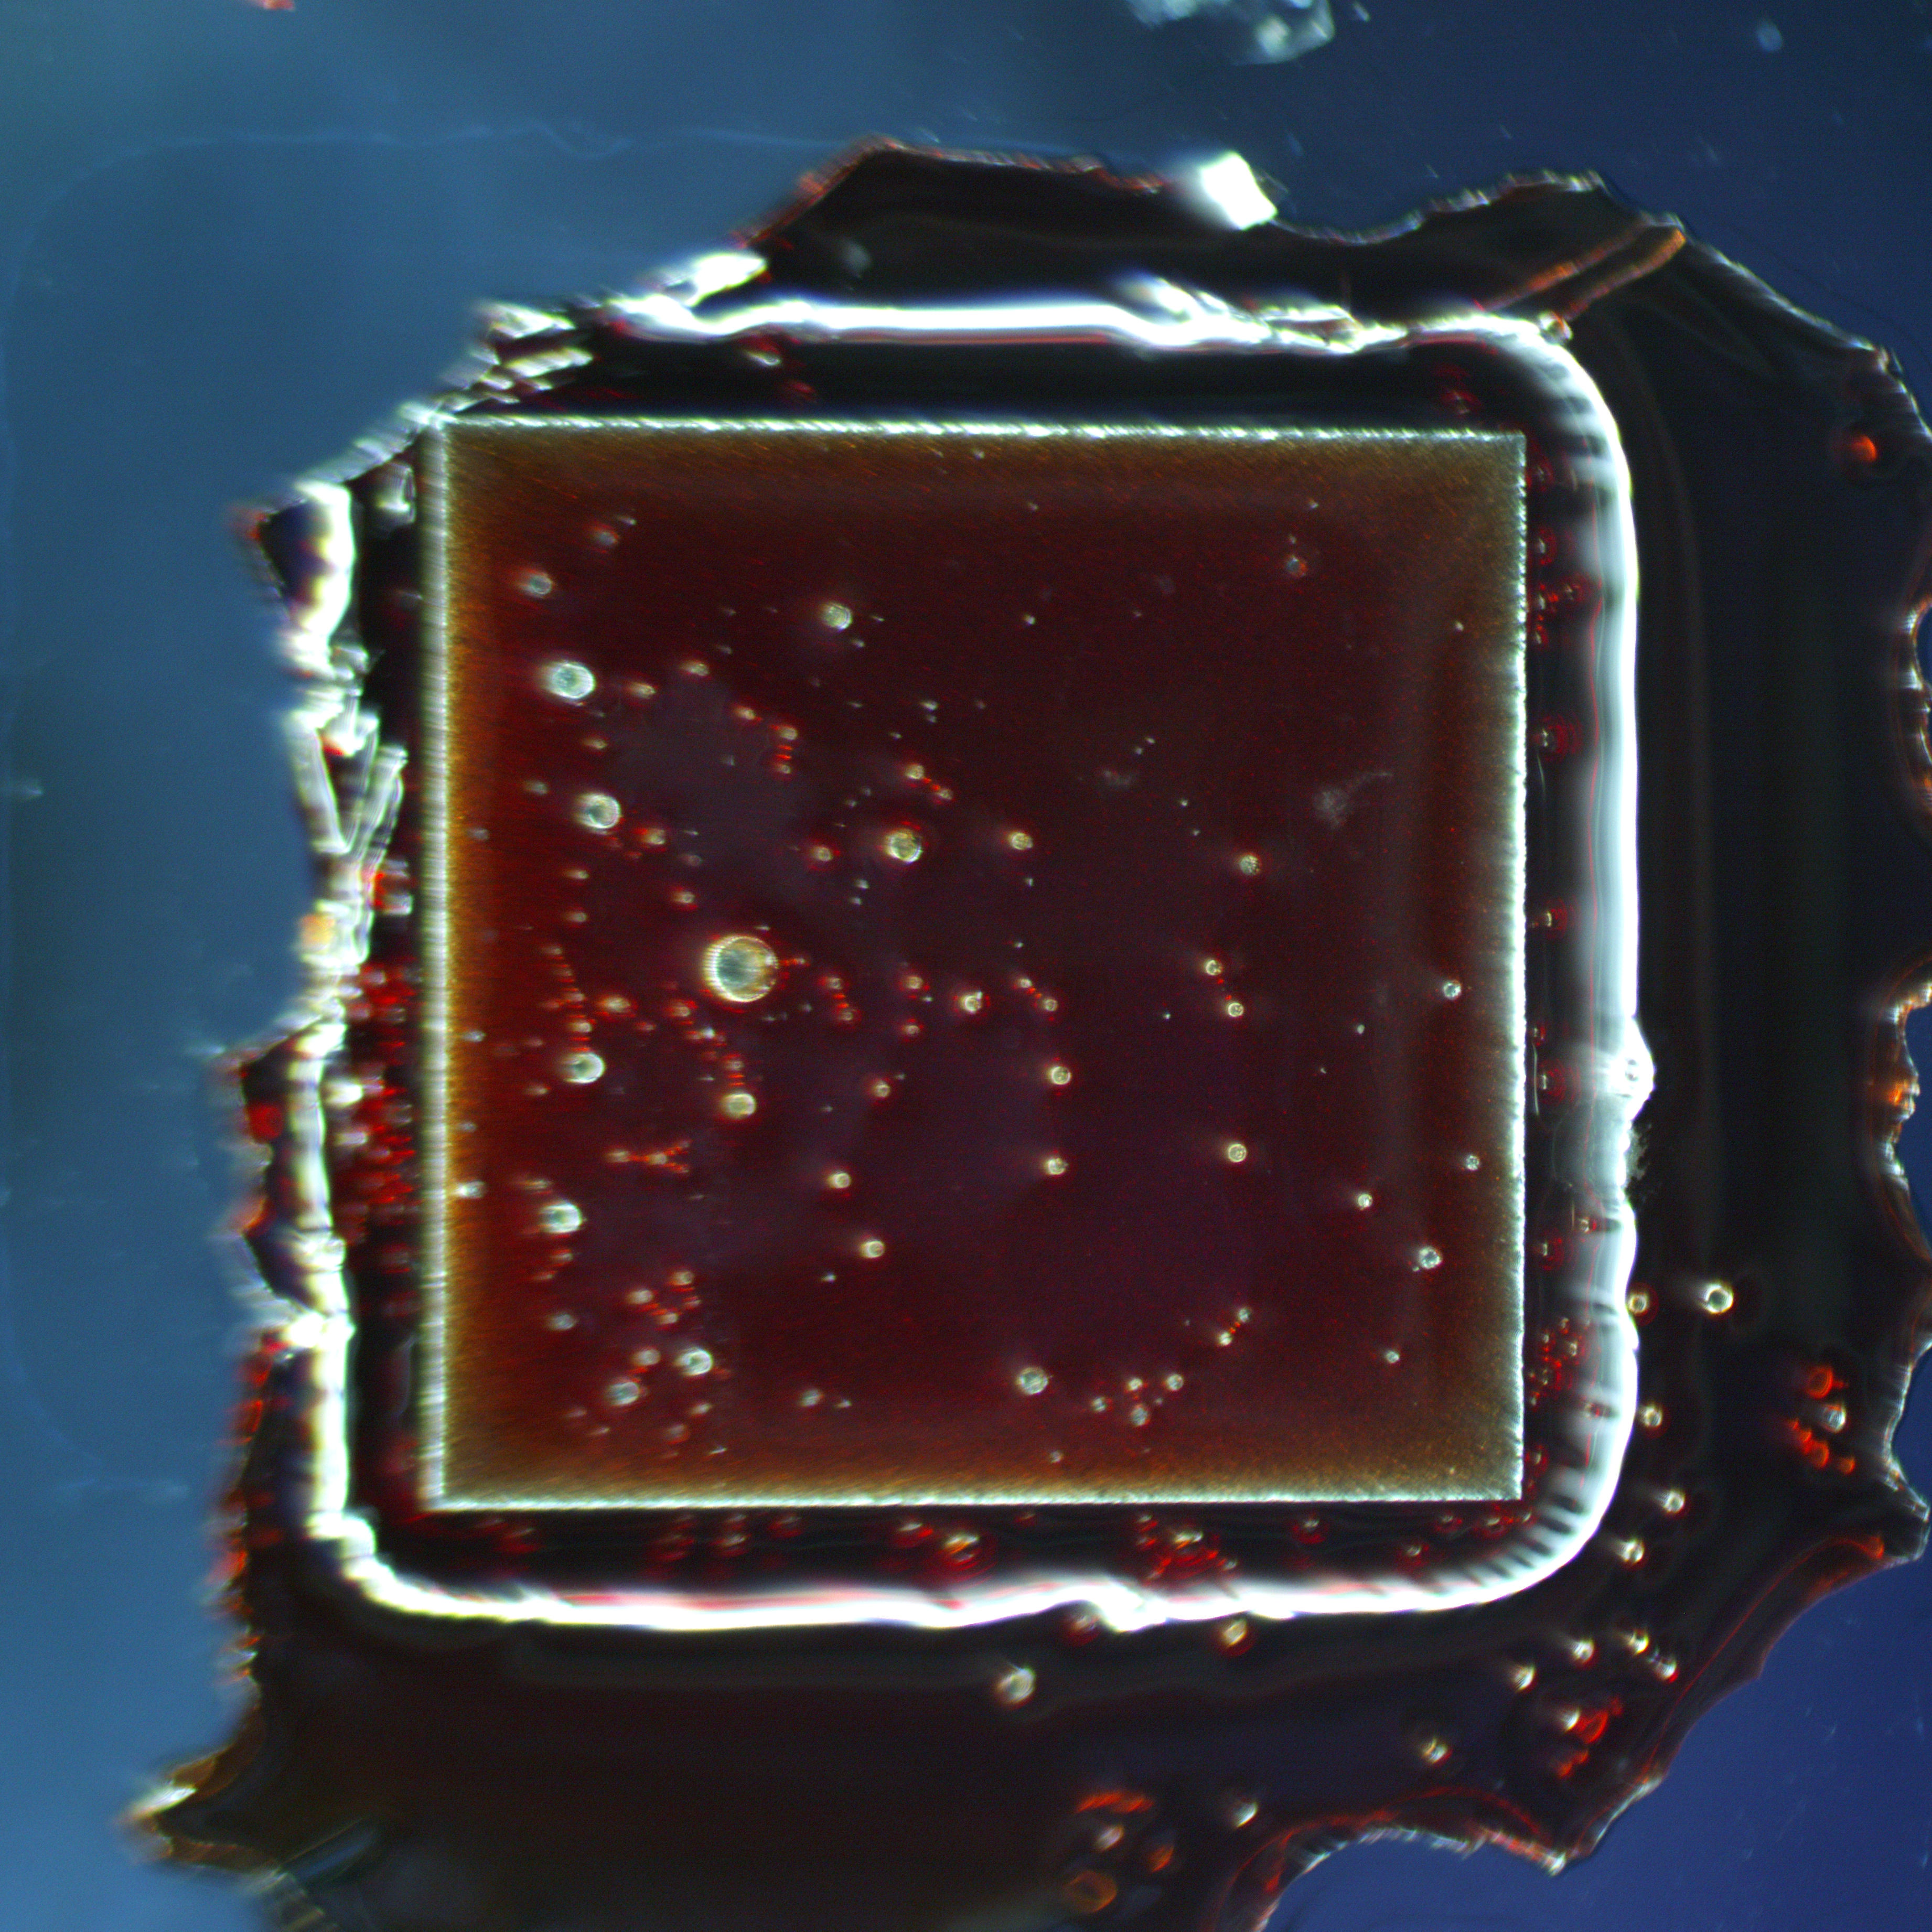
\includegraphics[width=\linewidth]{pics/spincoat/no12/12109.jpg}
        \caption{Heater 9}
    \end{subfigure}

    \caption[Optical Images of the Heater in Passivation Test \#12]{Optical images of the nine Heater of the coating test \#12. The two heaters that could be removed from the glue are highlighted in blue and the height measurement was taken of those marked by a "*"}
    \label{fig:PT12}
\end{figure}